\documentclass[twoside]{book}

% Packages required by doxygen
\usepackage{fixltx2e}
\usepackage{calc}
\usepackage{doxygen}
\usepackage[export]{adjustbox} % also loads graphicx
\usepackage{graphicx}
\usepackage[utf8]{inputenc}
\usepackage{makeidx}
\usepackage{multicol}
\usepackage{multirow}
\PassOptionsToPackage{warn}{textcomp}
\usepackage{textcomp}
\usepackage[nointegrals]{wasysym}
\usepackage[table]{xcolor}

% Font selection
\usepackage[T1]{fontenc}
\usepackage[scaled=.90]{helvet}
\usepackage{courier}
\usepackage{amssymb}
\usepackage{sectsty}
\renewcommand{\familydefault}{\sfdefault}
\allsectionsfont{%
  \fontseries{bc}\selectfont%
  \color{darkgray}%
}
\renewcommand{\DoxyLabelFont}{%
  \fontseries{bc}\selectfont%
  \color{darkgray}%
}
\newcommand{\+}{\discretionary{\mbox{\scriptsize$\hookleftarrow$}}{}{}}

% Page & text layout
\usepackage{geometry}
\geometry{%
  a4paper,%
  top=2.5cm,%
  bottom=2.5cm,%
  left=2.5cm,%
  right=2.5cm%
}
\tolerance=750
\hfuzz=15pt
\hbadness=750
\setlength{\emergencystretch}{15pt}
\setlength{\parindent}{0cm}
\setlength{\parskip}{3ex plus 2ex minus 2ex}
\makeatletter
\renewcommand{\paragraph}{%
  \@startsection{paragraph}{4}{0ex}{-1.0ex}{1.0ex}{%
    \normalfont\normalsize\bfseries\SS@parafont%
  }%
}
\renewcommand{\subparagraph}{%
  \@startsection{subparagraph}{5}{0ex}{-1.0ex}{1.0ex}{%
    \normalfont\normalsize\bfseries\SS@subparafont%
  }%
}
\makeatother

% Headers & footers
\usepackage{fancyhdr}
\pagestyle{fancyplain}
\fancyhead[LE]{\fancyplain{}{\bfseries\thepage}}
\fancyhead[CE]{\fancyplain{}{}}
\fancyhead[RE]{\fancyplain{}{\bfseries\leftmark}}
\fancyhead[LO]{\fancyplain{}{\bfseries\rightmark}}
\fancyhead[CO]{\fancyplain{}{}}
\fancyhead[RO]{\fancyplain{}{\bfseries\thepage}}
\fancyfoot[LE]{\fancyplain{}{}}
\fancyfoot[CE]{\fancyplain{}{}}
\fancyfoot[RE]{\fancyplain{}{\bfseries\scriptsize Generated by Doxygen }}
\fancyfoot[LO]{\fancyplain{}{\bfseries\scriptsize Generated by Doxygen }}
\fancyfoot[CO]{\fancyplain{}{}}
\fancyfoot[RO]{\fancyplain{}{}}
\renewcommand{\footrulewidth}{0.4pt}
\renewcommand{\chaptermark}[1]{%
  \markboth{#1}{}%
}
\renewcommand{\sectionmark}[1]{%
  \markright{\thesection\ #1}%
}

% Indices & bibliography
\usepackage{natbib}
\usepackage[titles]{tocloft}
\setcounter{tocdepth}{3}
\setcounter{secnumdepth}{5}
\makeindex

% Hyperlinks (required, but should be loaded last)
\usepackage{ifpdf}
\ifpdf
  \usepackage[pdftex,pagebackref=true]{hyperref}
\else
  \usepackage[ps2pdf,pagebackref=true]{hyperref}
\fi
\hypersetup{%
  colorlinks=true,%
  linkcolor=blue,%
  citecolor=blue,%
  unicode%
}

% Custom commands
\newcommand{\clearemptydoublepage}{%
  \newpage{\pagestyle{empty}\cleardoublepage}%
}

\usepackage{caption}
\captionsetup{labelsep=space,justification=centering,font={bf},singlelinecheck=off,skip=4pt,position=top}

%===== C O N T E N T S =====

\begin{document}

% Titlepage & ToC
\hypersetup{pageanchor=false,
             bookmarksnumbered=true,
             pdfencoding=unicode
            }
\pagenumbering{alph}
\begin{titlepage}
\vspace*{7cm}
\begin{center}%
{\Large robot\+\_\+interfaces }\\
\vspace*{1cm}
{\large Generated by Doxygen 1.8.13}\\
\end{center}
\end{titlepage}
\clearemptydoublepage
\pagenumbering{roman}
\tableofcontents
\clearemptydoublepage
\pagenumbering{arabic}
\hypersetup{pageanchor=true}

%--- Begin generated contents ---
\chapter{Robot Interfaces Documentation}
\label{index}\hypertarget{index}{}This is the documentation of the {\ttfamily robot\+\_\+fingers} package.

The source code is hosted on \href{https://github.com/open-dynamic-robot-initiative/robot_fingers}{\tt Git\+Hub}. Please also use the issue system there if you have a question or want to report a bug.

For more information, on the Tri\+Finger robot and the general architecture of the software, see also our \href{https://arxiv.org/abs/2008.03596}{\tt paper} on the open-\/source version of the Tri\+Finger robot.

\subsection*{Content }


\begin{DoxyItemize}
\item \hyperlink{md_doc_installation}{Build Instructions}
\item \hyperlink{md_doc_singularity}{About Singularity}
\item \hyperlink{md_doc_getting_started}{Getting Started}
\item \hyperlink{md_doc_hardware_testing}{Tools for Hardware Testing}
\end{DoxyItemize}

\subsection*{Links }


\begin{DoxyItemize}
\item \href{https://github.com/open-dynamic-robot-initiative/robot_fingers}{\tt Git\+Hub Repository}.
\item \href{https://github.com/open-dynamic-robot-initiative/robot_fingers/issues}{\tt Bug Tracker}.
\item This package implements a {\ttfamily Robot\+Driver} for the (Tri-\/)Finger robots based on our \href{https://open-dynamic-robot-initiative.github.io/code_documentation/robot_interfaces/docs/doxygen/html/index.html}{\tt {\ttfamily robot\+\_\+interfaces} package}. 
\end{DoxyItemize}
\chapter{How to Implement a Custom Robot\+Driver}
\label{md_docs_custom_driver}
\Hypertarget{md_docs_custom_driver}
To use robot\+\_\+interfaces with your own robot, you need to provide implementations for


\begin{DoxyItemize}
\item the Action type
\item the Observation type
\item the Robot\+Driver
\end{DoxyItemize}

\subsection*{Action and Observation }

Action and observation can be any arbitrary type, whatever is needed for your robot. There are only the following restrictions\+:


\begin{DoxyItemize}
\item If you want to use the \hyperlink{classrobot__interfaces_1_1MultiProcessRobotData}{robot\+\_\+interfaces\+::\+Multi\+Process\+Robot\+Data}, the action and observation types need to be serializable with \href{https://uscilab.github.io/cereal/}{\tt cereal}.
\item If you want to use the \hyperlink{classrobot__interfaces_1_1RobotLogger}{robot\+\_\+interfaces\+::\+Robot\+Logger}, the action and observation types need to inherit from \hyperlink{classrobot__interfaces_1_1Loggable}{robot\+\_\+interfaces\+::\+Loggable}.
\end{DoxyItemize}

\subsection*{Robot\+Driver }

Your robot driver needs to be a class that inherits from \hyperlink{classrobot__interfaces_1_1RobotDriver}{robot\+\_\+interfaces\+::\+Robot\+Driver}, using your {\ttfamily Action} and {\ttfamily Observation} types (see above).

\subsection*{Example }

See the example implementation of a dummy robot driver in \href{https://github.com/open-dynamic-robot-initiative/robot_interfaces/blob/master/include/robot_interfaces/example.hpp}{\tt example.\+hpp}. This dummy driver is also used in the \href{https://github.com/open-dynamic-robot-initiative/robot_interfaces/blob/master/demos}{\tt demos}. 
\chapter{Desired vs Applied Action}
\label{md_docs_desired_vs_applied_action}
\Hypertarget{md_docs_desired_vs_applied_action}
The action given by the user is called the {\itshape desired} action. Depending on the implementation of the \hyperlink{classrobot__interfaces_1_1RobotDriver}{robot\+\_\+interfaces\+::\+Robot\+Driver}, this action may be altered before it is actually applied on the robot, e.\+g. by some safety checks limiting torque and maximum velocity. This altered action is called the {\itshape applied} action. You can use \hyperlink{classrobot__interfaces_1_1RobotFrontend_a870651d849fe0f1a4909820cc3b6de40}{robot\+\_\+interfaces\+::\+Robot\+Frontend\+::get\+\_\+applied\+\_\+action} to see what action actually got applied on the robot. 
\chapter{Build Instructions}
\label{md_docs_installation}
\Hypertarget{md_docs_installation}
\begin{DoxyNote}{Note}
If you intend to use this interface to control your own robot, this package (and its dependencies) is enough, and you can follow the instructions below. If you are looking for the interface of the Tri\+Finger robot interface, see the installation instructions of the \href{https://open-dynamic-robot-initiative.github.io/code_documentation/robot_fingers/docs/doxygen/html/index.html}{\tt {\ttfamily robot\+\_\+fingers} package} instead (this also includes {\ttfamily robot\+\_\+interfaces}).
\end{DoxyNote}
\subsection*{Dependencies }

We are using \href{http://wiki.ros.org/catkin}{\tt catkin} as build tool (i.\+e. {\ttfamily robot\+\_\+interfaces} is a catkin package). While we are not really depending on any \href{http://www.ros.org}{\tt R\+OS} packages, this means you need a basic R\+OS installation to build.

In the following we are using catkin\+\_\+tools which need to be installed separately\+: \begin{DoxyVerb}pip install catkin_tools
\end{DoxyVerb}


We are testing on Ubuntu 18.\+04 with R\+OS Melodic. Other versions may work as well but are not officially supported.

\begin{DoxyNote}{Note}
We provide a Singularity image with all dependencies for the Tri\+Finger robot which also covers everything needed for {\ttfamily robot\+\_\+interfaces}. See the documentation of the \href{https://open-dynamic-robot-initiative.github.io/code_documentation/robot_fingers/docs/doxygen/html/index.html}{\tt {\ttfamily robot\+\_\+fingers} package} for more information.
\end{DoxyNote}
\subsection*{Get the Source }

{\ttfamily robot\+\_\+interfaces} depends on several other of our packages which are organized in separate repositories. We therefore use a workspace management tool called \href{https://pypi.org/project/treep/}{\tt treep} which allows easy cloning of multi-\/repository projects.

treep can be installed via pip\+: \begin{DoxyVerb}pip install treep
\end{DoxyVerb}


Clone the treep configuration containing the \char`\"{}\+R\+O\+B\+O\+T\+\_\+\+I\+N\+T\+E\+R\+F\+A\+C\+E\+S\char`\"{} project\+: \begin{DoxyVerb}git clone git@github.com:machines-in-motion/treep_machines_in_motion.git
\end{DoxyVerb}


\begin{DoxyNote}{Note}
treep searches for a configuration directory from the current working directory upwards. So you can use treep in the directory in which you invoked the {\ttfamily git clone} command above or any subdirectory.
\end{DoxyNote}
Now clone the project\+: \begin{DoxyVerb}treep --clone ROBOT_INTERFACES
\end{DoxyVerb}


\begin{DoxyNote}{Note}
{\bfseries Important\+:} treep uses S\+SH to clone from github. So for the above command to work, you need a github account with a registered S\+SH key. Further this key needs to work without asking for a password everytime. To achieve this, run \begin{DoxyVerb}ssh-add
\end{DoxyVerb}

\end{DoxyNote}
first.

You should now have the following directory structure\+: \begin{DoxyVerb}├── treep_machines_in_motion
└── workspace
    └── src
        ├── catkin
        │   ├── core_robotics
        │   │   ├── mpi_cmake_modules
        │   │   ├── pybind11_catkin
        │   │   ├── real_time_tools
        │   │   ├── shared_memory
        │   │   ├── time_series
        │   │   └── yaml_cpp_catkin
        │   ├── examples
        │   │   └── ci_example
        │   ├── robots
        │   │   └── robot_interfaces
        │   └── tools
        │       ├── serialization_utils
        │       └── signal_handler
        └── not_catkin
            └── third_party
                └── pybind11
\end{DoxyVerb}


\subsection*{Build }

To build, cd into the {\ttfamily workspace} directory and call \begin{DoxyVerb}catkin build
\end{DoxyVerb}


to build the whole workspace.

\subsubsection*{Python Bindings}

With the above command Python bindings will be build for the default python version of your system (see {\ttfamily python -\/-\/version}). If you want to use a different version (e.\+g. python3), you can specify as follows\+: \begin{DoxyVerb}catkin build -DPYTHON_EXECUTABLE=/usr/bin/python3\end{DoxyVerb}
 
\chapter{Quick Start Example}
\label{md_docs_quick_start_example}
\Hypertarget{md_docs_quick_start_example}
Sending actions to and getting observations from the robot is very easy. See the following example, using the Tri\+Finger robot, that simply sends a constant position command.

\begin{DoxyNote}{Note}
This example shows only the frontend part of a multi-\/process setup. The backend for the actual robot needs to be run in a separate process.
\end{DoxyNote}
\subsection*{Python}


\begin{DoxyCode}
\textcolor{keyword}{import} robot\_interfaces

robot\_data = robot\_interfaces.trifinger.MultiProcessData(
    \textcolor{stringliteral}{"trifinger"}, \textcolor{keyword}{False})
frontend = robot\_interfaces.trifinger.Frontend(robot\_data)

position = [
     0.0,  \textcolor{comment}{# Finger 1, Upper Joint}
    -0.9,  \textcolor{comment}{# Finger 1, Middle Joint}
    -1.7,  \textcolor{comment}{# Finger 1, Lower Joint}
     0.0,  \textcolor{comment}{# Finger 2, Upper Joint}
    -0.9,  \textcolor{comment}{# Finger 2, Middle Joint}
    -1.7,  \textcolor{comment}{# Finger 2, Lower Joint}
     0.0,  \textcolor{comment}{# Finger 3, Upper Joint}
    -0.9,  \textcolor{comment}{# Finger 3, Middle Joint}
    -1.7,  \textcolor{comment}{# Finger 3, Lower Joint}
]

\textcolor{keywordflow}{while} \textcolor{keyword}{True}:
    \textcolor{comment}{# construct an action with a position command}
    action = robot\_interfaces.trifinger.Action(position=position)
    \textcolor{comment}{# send the action to the robot (will be applied in time step t)}
    t = frontend.append\_desired\_action(action)
    \textcolor{comment}{# wait until time step t and get observation}
    observation = frontend.get\_observation(t)

    print(\textcolor{stringliteral}{"Observed Position: \{\}"}.format(observation.position))
\end{DoxyCode}


\subsection*{C++}


\begin{DoxyCode}
\textcolor{preprocessor}{#include <robot\_interfaces/finger\_types.hpp>}

\textcolor{comment}{// Some convenience typedefs to make the code below more compact}
\textcolor{keyword}{typedef} \hyperlink{classrobot__interfaces_1_1MultiProcessRobotData}{robot\_interfaces::TriFingerTypes::MultiProcessData}
       RobotData;
\textcolor{keyword}{typedef} \hyperlink{classrobot__interfaces_1_1RobotFrontend}{robot\_interfaces::TriFingerTypes::Frontend} RobotFrontend;
\textcolor{keyword}{typedef} \hyperlink{structrobot__interfaces_1_1NJointAction}{robot\_interfaces::TriFingerTypes::Action} Action;

\textcolor{keywordtype}{int} main()
\{
    \textcolor{keyword}{auto} robot\_data = std::make\_shared<RobotData>(\textcolor{stringliteral}{"trifinger"}, \textcolor{keyword}{false});
    \textcolor{keyword}{auto} frontend = RobotFrontend(robot\_data);

    Action::Vector position;  \textcolor{comment}{// <- this is an "Eigen::Vector9d"}
    position <<  0.0,  \textcolor{comment}{// Finger 1, Upper Joint}
                -0.9,  \textcolor{comment}{// Finger 1, Middle Joint}
                -1.7,  \textcolor{comment}{// Finger 1, Lower Joint}
                 0.0,  \textcolor{comment}{// Finger 2, Upper Joint}
                -0.9,  \textcolor{comment}{// Finger 2, Middle Joint}
                -1.7,  \textcolor{comment}{// Finger 2, Lower Joint}
                 0.0,  \textcolor{comment}{// Finger 3, Upper Joint}
                -0.9,  \textcolor{comment}{// Finger 3, Middle Joint}
                -1.7;  \textcolor{comment}{// Finger 3, Lower Joint}

    \textcolor{keywordflow}{while} (\textcolor{keyword}{true})
    \{
        \textcolor{comment}{// construct an action with a position command}
        Action action = Action::Position(position);
        \textcolor{comment}{// send the action to the robot (will be applied in time step t)}
        \textcolor{keyword}{auto} t = frontend.append\_desired\_action(action);
        \textcolor{comment}{// wait until time step t and get observation}
        \textcolor{keyword}{auto} observation = frontend.get\_observation(t);

        std::cout << \textcolor{stringliteral}{"Observed Position: "}
                  << observation.position
                  << std::endl;
    \}

    \textcolor{keywordflow}{return} 0;
\}
\end{DoxyCode}


When using C++ you need to add the package {\ttfamily robot\+\_\+interfaces} as build dependency to your package.

\subsection*{More Examples}

For more examples, see the \href{https://github.com/open-dynamic-robot-initiative/robot_interfaces/tree/master/demos}{\tt C++ demos of the {\ttfamily robot\+\_\+interfaces} package} and the \href{https://github.com/open-dynamic-robot-initiative/robot_fingers/tree/master/demos}{\tt Python demos in the {\ttfamily robot\+\_\+fingers} package}. 
\chapter{Robot\+Data -\/-\/ Single or Multi Process}
\label{md_docs_robot_data}
\Hypertarget{md_docs_robot_data}
The \hyperlink{classrobot__interfaces_1_1RobotData}{Robot\+Data} class serves as a communication link between the back end and the front end. All data is stored there in time series.

There are two different implementations of {\ttfamily Robot\+Data}\+:


\begin{DoxyItemize}
\item \hyperlink{classrobot__interfaces_1_1SingleProcessRobotData}{Single\+Process\+Robot\+Data}\+: Uses normal memory for the time series. Use this if all modules (back end, front end, logger, ...) are running in the same process.
\item \hyperlink{classrobot__interfaces_1_1MultiProcessRobotData}{Multi\+Process\+Robot\+Data}\+: Uses shared memory for inter-\/process communication. Use this if back end and front end are running in separate processes.
\end{DoxyItemize}

See the \href{https://github.com/open-dynamic-robot-initiative/robot_interfaces/blob/master/demos}{\tt demos} for implementations with both the single and the multi process Robot\+Data. 
\chapter{Logic of Actions and Observations}
\label{md_docs_timeseries}
\Hypertarget{md_docs_timeseries}
In this section the logic of the {\itshape time series} used for communication between front and back end and for synchronization between actions and observations is explained. For more details, please see our \href{https://arxiv.org/abs/2008.03596}{\tt paper} on the open-\/source version of the Tri\+Finger robot.

\subsection*{On Time Series and Time Relation of Actions and Observations }

All data transfer between the front end (= user code) and the back end (= robot hardware) goes through so called time series. When calling {\ttfamily append\+\_\+desired\+\_\+action(action)}, the action is not applied immediately but is {\itshape appended} to the time series of desired actions which serves as a queue.

At each time step, identified by a {\itshape time index t}, the backend takes the action at position {\itshape t} from the \char`\"{}desired actions\char`\"{} time series and sends it to the robot driver. At the same time an observation is acquired from the robot and added to the \char`\"{}observation\char`\"{} time series. This means that the effect of the desired action {\ttfamily a\+\_\+t} is not yet visible in the observation {\ttfamily y\+\_\+t} as is illustrated below. (`a\textquotesingle{}\+\_\+t` corresponds to the {\itshape applied action}, see \hyperlink{md_docs_desired_vs_applied_action}{Desired vs Applied Action})



{\ttfamily append\+\_\+desired\+\_\+action()} returns the time index {\ttfamily t} at which the appended action will be executed. Methods like {\ttfamily get\+\_\+observation()} expect a time index as input. If the specified time step has already passed, they immediately return the value from the corresponding step. If it lies in the future, the method will block and wait until the specified time step is reached and then return.

Note that the buffer size of the time series is limited (see the {\ttfamily history\+\_\+length} argument of {\ttfamily Single\+Process\+Robot\+Data} and {\ttfamily Multi\+Process\+Robot\+Data}). If the buffer is full, the oldest element is discarded. Trying to access an time index that is not in the buffer anymore results in an exception.

This design allows for simple code that is automatically executed at the control rate of the robot\+:


\begin{DoxyCode}
\textcolor{comment}{# send zero-torque action to get first observation, see explanation below}
zero\_torque\_action = robot\_interfaces.trifinger.Action()
t = frontend.append\_desired\_action(zero\_torque\_action)
observation = frontend.get\_observation(t)

\textcolor{keywordflow}{while} \textcolor{keyword}{True}:
    action = smart\_algorithm\_to\_compute\_next\_action(observation)

    t = frontend.append\_desired\_action(action)
    \textcolor{comment}{# The t given above refers to the moment the given action will be}
    \textcolor{comment}{# executed.  Right now, this is in the future, so the following call}
    \textcolor{comment}{# will automatically wait until the action is actually applied to the}
    \textcolor{comment}{# platform}
    observation = frontend.get\_observation(t)
\end{DoxyCode}


\subsubsection*{Send Action to Start Backend}

In the beginning of the program execution, the back end is idle and waiting for the first action. Only after the first action is received, the loop is started that applies actions and writes observations to the time series.

This means {\bfseries you first have to send an action before you can read the first observation!}

There are applications where an observation is needed before sending the first real action (e.\+g. when the action depends on the current position). In this case you need to send a \char`\"{}neutral\char`\"{} action first. How this action may look is robot dependent. The {\itshape Tri\+Finger} robot, for example, can safely be started with a zero-\/torque action\+:

Python\+:


\begin{DoxyCode}
\textcolor{comment}{# an action without arguments defaults to zero torque}
zero\_torque\_action = robot\_interfaces.trifinger.Action()
t = frontend.append\_desired\_action(zero\_torque\_action)
first\_observation = frontend.get\_observation(t)
\end{DoxyCode}


C++\+:


\begin{DoxyCode}
Action zero\_torque\_action = Action::Zero();
\textcolor{keyword}{auto} t = frontend.append\_desired\_action(zero\_torque\_action);
\textcolor{keyword}{auto} first\_observation = frontend.get\_observation(t);
\end{DoxyCode}


Note that the creation of the zero torque action in the above example is specific to the {\itshape Tri\+Finger} robot. For other robots, the creation of the action would need to be adjusted to the action type of that specific robot.

If the back end reaches a time step {\ttfamily t} but the user did not yet provide an action for this time step (e.\+g. because the user code is running slower than 1 k\+Hz), the back end automatically sets the desired action for step {\ttfamily t} to the same as the one of {\ttfamily t -\/ 1}.

This is indicated to the user through the {\ttfamily action\+\_\+repetitions} field in the status message which contains the number of times the current action has been repeated. 
\chapter{Robot interfaces}
\label{md_readme}
\Hypertarget{md_readme}
\subsection*{What is it}

Interface using internet connexion to a A\+TI force torque sensor.

\subsection*{Authors}

Ludovic Righetti Alexander Herzog

\subsection*{Copyrights}

Copyright (c) 2019, New York University and Max Planck Gesellschaft.

\subsection*{License}

License B\+S\+D-\/3-\/\+Clause 
\chapter{Deprecated List}
\label{deprecated}
\Hypertarget{deprecated}

\begin{DoxyRefList}
\item[\label{deprecated__deprecated000001}%
\Hypertarget{deprecated__deprecated000001}%
Member \hyperlink{classblmc__robots_1_1BlmcJointModule_a17a1da041dae31e9a16f955722c36d6c}{blmc\+\_\+robots\+:\+:Blmc\+Joint\+Module\+:\+:calibrate} (double \&angle\+\_\+zero\+\_\+to\+\_\+index, double \&index\+\_\+angle, bool mechanical\+\_\+calibration=false)]!!!!!!! 
\end{DoxyRefList}
\chapter{License}
\label{license}
\Hypertarget{license}

\begin{DoxyRefList}
\item[\label{license__license000001}%
\Hypertarget{license__license000001}%
File \hyperlink{n__finger__driver_8hpp}{n\+\_\+finger\+\_\+driver.hpp} ]B\+SD 3-\/clause  
\item[\label{license__license000003}%
\Hypertarget{license__license000003}%
File \hyperlink{trifinger__platform__frontend_8cpp}{trifinger\+\_\+platform\+\_\+frontend.cpp} ]B\+SD 3-\/clause  
\item[\label{license__license000002}%
\Hypertarget{license__license000002}%
File \hyperlink{trifinger__platform__frontend_8hpp}{trifinger\+\_\+platform\+\_\+frontend.hpp} ]B\+SD 3-\/clause 
\end{DoxyRefList}
\chapter{Hierarchical Index}
\section{Class Hierarchy}
This inheritance list is sorted roughly, but not completely, alphabetically\+:\begin{DoxyCompactList}
\item \contentsline{section}{trifinger\+\_\+simulation.\+action.\+Action}{\pageref{classtrifinger__simulation_1_1action_1_1Action}}{}
\item \contentsline{section}{trifinger\+\_\+simulation.\+collision\+\_\+objects.\+Block}{\pageref{classtrifinger__simulation_1_1collision__objects_1_1Block}}{}
\item \contentsline{section}{trifinger\+\_\+simulation.\+trifinger\+\_\+platform.\+Camera\+Observation}{\pageref{classtrifinger__simulation_1_1trifinger__platform_1_1CameraObservation}}{}
\item \contentsline{section}{trifinger\+\_\+simulation.\+visual\+\_\+objects.\+Cube\+Marker}{\pageref{classtrifinger__simulation_1_1visual__objects_1_1CubeMarker}}{}
\item \contentsline{section}{trifinger\+\_\+simulation.\+gym\+\_\+wrapper.\+data\+\_\+logger.\+Data\+Logger}{\pageref{classtrifinger__simulation_1_1gym__wrapper_1_1data__logger_1_1DataLogger}}{}
\item Env\begin{DoxyCompactList}
\item \contentsline{section}{example\+\_\+pushing\+\_\+training\+\_\+env.\+Example\+Pushing\+Training\+Env}{\pageref{classexample__pushing__training__env_1_1ExamplePushingTrainingEnv}}{}
\item \contentsline{section}{trifinger\+\_\+simulation.\+gym\+\_\+wrapper.\+envs.\+trifinger\+\_\+push.\+Tri\+Finger\+Push}{\pageref{classtrifinger__simulation_1_1gym__wrapper_1_1envs_1_1trifinger__push_1_1TriFingerPush}}{}
\item \contentsline{section}{trifinger\+\_\+simulation.\+gym\+\_\+wrapper.\+envs.\+trifinger\+\_\+reach.\+Tri\+Finger\+Reach}{\pageref{classtrifinger__simulation_1_1gym__wrapper_1_1envs_1_1trifinger__reach_1_1TriFingerReach}}{}
\end{DoxyCompactList}
\item \contentsline{section}{trifinger\+\_\+simulation.\+gym\+\_\+wrapper.\+data\+\_\+logger.\+Episode\+Data}{\pageref{classtrifinger__simulation_1_1gym__wrapper_1_1data__logger_1_1EpisodeData}}{}
\item Exception\begin{DoxyCompactList}
\item \contentsline{section}{trifinger\+\_\+simulation.\+tasks.\+move\+\_\+cube.\+Invalid\+Goal\+Error}{\pageref{classtrifinger__simulation_1_1tasks_1_1move__cube_1_1InvalidGoalError}}{}
\end{DoxyCompactList}
\item \contentsline{section}{trifinger\+\_\+simulation.\+gym\+\_\+wrapper.\+finger\+\_\+spaces.\+Finger\+Spaces}{\pageref{classtrifinger__simulation_1_1gym__wrapper_1_1finger__spaces_1_1FingerSpaces}}{}
\item \contentsline{section}{trifinger\+\_\+simulation.\+visual\+\_\+objects.\+Marker}{\pageref{classtrifinger__simulation_1_1visual__objects_1_1Marker}}{}
\item Named\+Tuple\begin{DoxyCompactList}
\item \contentsline{section}{run\+\_\+evaluate\+\_\+policy\+\_\+all\+\_\+levels.\+Test\+Sample}{\pageref{classrun__evaluate__policy__all__levels_1_1TestSample}}{}
\item \contentsline{section}{run\+\_\+replay\+\_\+all\+\_\+levels.\+Test\+Sample}{\pageref{classrun__replay__all__levels_1_1TestSample}}{}
\item \contentsline{section}{trifinger\+\_\+simulation.\+finger\+\_\+types\+\_\+data.\+Finger\+Types\+Data\+Format}{\pageref{classtrifinger__simulation_1_1finger__types__data_1_1FingerTypesDataFormat}}{}
\end{DoxyCompactList}
\item object\begin{DoxyCompactList}
\item \contentsline{section}{trifinger\+\_\+simulation.\+camera.\+Camera}{\pageref{classtrifinger__simulation_1_1camera_1_1Camera}}{}
\end{DoxyCompactList}
\item \contentsline{section}{trifinger\+\_\+simulation.\+trifinger\+\_\+platform.\+Object\+Pose}{\pageref{classtrifinger__simulation_1_1trifinger__platform_1_1ObjectPose}}{}
\item \contentsline{section}{trifinger\+\_\+simulation.\+observation.\+Observation}{\pageref{classtrifinger__simulation_1_1observation_1_1Observation}}{}
\item Observation\+Wrapper\begin{DoxyCompactList}
\item \contentsline{section}{example\+\_\+pushing\+\_\+training\+\_\+env.\+Flat\+Observation\+Wrapper}{\pageref{classexample__pushing__training__env_1_1FlatObservationWrapper}}{}
\end{DoxyCompactList}
\item \contentsline{section}{trifinger\+\_\+simulation.\+pinocchio\+\_\+utils.\+Pinocchio\+Utils}{\pageref{classtrifinger__simulation_1_1pinocchio__utils_1_1PinocchioUtils}}{}
\item \contentsline{section}{trifinger\+\_\+simulation.\+tasks.\+move\+\_\+cube.\+Pose}{\pageref{classtrifinger__simulation_1_1tasks_1_1move__cube_1_1Pose}}{}
\item \contentsline{section}{evaluate\+\_\+policy.\+P\+P\+O\+Policy}{\pageref{classevaluate__policy_1_1PPOPolicy}}{}
\item \contentsline{section}{evaluate\+\_\+policy.\+Random\+Policy}{\pageref{classevaluate__policy_1_1RandomPolicy}}{}
\item \contentsline{section}{demo\+\_\+random\+\_\+policy.\+Random\+Policy}{\pageref{classdemo__random__policy_1_1RandomPolicy}}{}
\item \contentsline{section}{trifinger\+\_\+simulation.\+real\+\_\+finger.\+Real\+Finger}{\pageref{classtrifinger__simulation_1_1real__finger_1_1RealFinger}}{}
\item Robot\+Driver\begin{DoxyCompactList}
\item \contentsline{section}{trifinger\+\_\+simulation\+:\+:Base\+Py\+Bullet\+Finger\+Driver$<$ robot\+\_\+interfaces\+:\+:Mono\+Finger\+Types\+:\+:Action, robot\+\_\+interfaces\+:\+:Mono\+Finger\+Types\+:\+:Observation $>$}{\pageref{classtrifinger__simulation_1_1BasePyBulletFingerDriver}}{}
\begin{DoxyCompactList}
\item \contentsline{section}{trifinger\+\_\+simulation\+:\+:Py\+Bullet\+Single\+Finger\+Driver}{\pageref{classtrifinger__simulation_1_1PyBulletSingleFingerDriver}}{}
\end{DoxyCompactList}
\item \contentsline{section}{trifinger\+\_\+simulation\+:\+:Base\+Py\+Bullet\+Finger\+Driver$<$ robot\+\_\+interfaces\+:\+:Tri\+Finger\+Types\+:\+:Action, robot\+\_\+interfaces\+:\+:Tri\+Finger\+Types\+:\+:Observation $>$}{\pageref{classtrifinger__simulation_1_1BasePyBulletFingerDriver}}{}
\begin{DoxyCompactList}
\item \contentsline{section}{trifinger\+\_\+simulation\+:\+:Py\+Bullet\+Tri\+Finger\+Driver}{\pageref{classtrifinger__simulation_1_1PyBulletTriFingerDriver}}{}
\end{DoxyCompactList}
\item \contentsline{section}{trifinger\+\_\+simulation\+:\+:Base\+Py\+Bullet\+Finger\+Driver$<$ Action, Observation $>$}{\pageref{classtrifinger__simulation_1_1BasePyBulletFingerDriver}}{}
\end{DoxyCompactList}
\item \contentsline{section}{trifinger\+\_\+simulation.\+sim\+\_\+finger.\+Sim\+Finger}{\pageref{classtrifinger__simulation_1_1sim__finger_1_1SimFinger}}{}
\item \contentsline{section}{trifinger\+\_\+simulation.\+trifinger\+\_\+platform.\+Tri\+Camera\+Observation}{\pageref{classtrifinger__simulation_1_1trifinger__platform_1_1TriCameraObservation}}{}
\item \contentsline{section}{trifinger\+\_\+simulation.\+camera.\+Tri\+Finger\+Cameras}{\pageref{classtrifinger__simulation_1_1camera_1_1TriFingerCameras}}{}
\item \contentsline{section}{trifinger\+\_\+simulation.\+trifinger\+\_\+platform.\+Tri\+Finger\+Platform}{\pageref{classtrifinger__simulation_1_1trifinger__platform_1_1TriFingerPlatform}}{}
\end{DoxyCompactList}

\chapter{Class Index}
\section{Class List}
Here are the classes, structs, unions and interfaces with brief descriptions\+:\begin{DoxyCompactList}
\item\contentsline{section}{\hyperlink{classrobot__properties__solo_1_1quadruped12wrapper_1_1Quadruped12Robot}{robot\+\_\+properties\+\_\+solo.\+quadruped12wrapper.\+Quadruped12\+Robot} }{\pageref{classrobot__properties__solo_1_1quadruped12wrapper_1_1Quadruped12Robot}}{}
\item\contentsline{section}{\hyperlink{classrobot__properties__solo_1_1config_1_1Solo12Config}{robot\+\_\+properties\+\_\+solo.\+config.\+Solo12\+Config} }{\pageref{classrobot__properties__solo_1_1config_1_1Solo12Config}}{}
\item\contentsline{section}{\hyperlink{classrobot__properties__solo_1_1solo8wrapper_1_1Solo8Robot}{robot\+\_\+properties\+\_\+solo.\+solo8wrapper.\+Solo8\+Robot} }{\pageref{classrobot__properties__solo_1_1solo8wrapper_1_1Solo8Robot}}{}
\item\contentsline{section}{\hyperlink{classrobot__properties__solo_1_1config_1_1SoloAbstract}{robot\+\_\+properties\+\_\+solo.\+config.\+Solo\+Abstract} \\*Abstract class used for all Solo robots }{\pageref{classrobot__properties__solo_1_1config_1_1SoloAbstract}}{}
\item\contentsline{section}{\hyperlink{classrobot__properties__solo_1_1config_1_1SoloConfig}{robot\+\_\+properties\+\_\+solo.\+config.\+Solo\+Config} }{\pageref{classrobot__properties__solo_1_1config_1_1SoloConfig}}{}
\end{DoxyCompactList}

\chapter{File Index}
\section{File List}
Here is a list of all documented files with brief descriptions\+:\begin{DoxyCompactList}
\item\contentsline{section}{include/\hyperlink{AtiFTSensor_8h}{Ati\+F\+T\+Sensor.\+h} }{\pageref{AtiFTSensor_8h}}{}
\end{DoxyCompactList}

\chapter{Class Documentation}
\hypertarget{classrobot__interfaces_1_1demo_1_1Action}{}\section{robot\+\_\+interfaces\+:\+:demo\+:\+:Action Class Reference}
\label{classrobot__interfaces_1_1demo_1_1Action}\index{robot\+\_\+interfaces\+::demo\+::\+Action@{robot\+\_\+interfaces\+::demo\+::\+Action}}


Actions to be performed by robot, will be received by \hyperlink{classDriver}{Driver}.  




{\ttfamily \#include $<$types.\+hpp$>$}

\subsection*{Public Member Functions}
\begin{DoxyCompactItemize}
\item 
\mbox{\Hypertarget{classrobot__interfaces_1_1demo_1_1Action_a67995830d81cf6c80ae61fa1436d8670}\label{classrobot__interfaces_1_1demo_1_1Action_a67995830d81cf6c80ae61fa1436d8670}} 
void {\bfseries print} (bool backline) const
\item 
\mbox{\Hypertarget{classrobot__interfaces_1_1demo_1_1Action_ae26340c1f9b73b3bd4c447572b16f1bf}\label{classrobot__interfaces_1_1demo_1_1Action_ae26340c1f9b73b3bd4c447572b16f1bf}} 
{\footnotesize template$<$class Archive $>$ }\\void {\bfseries serialize} (Archive \&ar)
\end{DoxyCompactItemize}
\subsection*{Public Attributes}
\begin{DoxyCompactItemize}
\item 
\mbox{\Hypertarget{classrobot__interfaces_1_1demo_1_1Action_a548fc6556545cd207c10391c8059b57a}\label{classrobot__interfaces_1_1demo_1_1Action_a548fc6556545cd207c10391c8059b57a}} 
int {\bfseries values} \mbox{[}2\mbox{]}
\end{DoxyCompactItemize}


\subsection{Detailed Description}
Actions to be performed by robot, will be received by \hyperlink{classDriver}{Driver}. 

An action simply encapsulate two desired position value, one for each dof \begin{Desc}
\item[Examples\+: ]\par
\hyperlink{demo_multiprocess_backend_8cpp-example}{demo\+\_\+multiprocess\+\_\+backend.\+cpp}, and \hyperlink{demo_multiprocess_frontend_8cpp-example}{demo\+\_\+multiprocess\+\_\+frontend.\+cpp}.\end{Desc}


The documentation for this class was generated from the following file\+:\begin{DoxyCompactItemize}
\item 
demos/\hyperlink{demos_2types_8hpp}{types.\+hpp}\end{DoxyCompactItemize}

\hypertarget{classrobot__interfaces_1_1example_1_1Action}{}\section{robot\+\_\+interfaces\+:\+:example\+:\+:Action Class Reference}
\label{classrobot__interfaces_1_1example_1_1Action}\index{robot\+\_\+interfaces\+::example\+::\+Action@{robot\+\_\+interfaces\+::example\+::\+Action}}


Actions to be performed by robot, will be received by \hyperlink{classrobot__interfaces_1_1example_1_1Driver}{Driver}.  




{\ttfamily \#include $<$example.\+hpp$>$}

\subsection*{Public Member Functions}
\begin{DoxyCompactItemize}
\item 
\mbox{\Hypertarget{classrobot__interfaces_1_1example_1_1Action_aafdd1a4294fb59562470365069998489}\label{classrobot__interfaces_1_1example_1_1Action_aafdd1a4294fb59562470365069998489}} 
void {\bfseries print} (bool backline)
\end{DoxyCompactItemize}
\subsection*{Public Attributes}
\begin{DoxyCompactItemize}
\item 
\mbox{\Hypertarget{classrobot__interfaces_1_1example_1_1Action_ae257ddae63338cf7bcc63d199a130098}\label{classrobot__interfaces_1_1example_1_1Action_ae257ddae63338cf7bcc63d199a130098}} 
int {\bfseries values} \mbox{[}2\mbox{]}
\end{DoxyCompactItemize}


\subsection{Detailed Description}
Actions to be performed by robot, will be received by \hyperlink{classrobot__interfaces_1_1example_1_1Driver}{Driver}. 

An action simply encapsulate two desired position value, one for each D\+OF. \begin{Desc}
\item[Examples\+: ]\par
\hyperlink{demo_8cpp-example}{demo.\+cpp}.\end{Desc}


The documentation for this class was generated from the following file\+:\begin{DoxyCompactItemize}
\item 
include/robot\+\_\+interfaces/\hyperlink{example_8hpp}{example.\+hpp}\end{DoxyCompactItemize}

\hypertarget{structrobot__interfaces_1_1BindTipForceIfExists}{}\section{robot\+\_\+interfaces\+:\+:Bind\+Tip\+Force\+If\+Exists$<$ Types, typename $>$ Struct Template Reference}
\label{structrobot__interfaces_1_1BindTipForceIfExists}\index{robot\+\_\+interfaces\+::\+Bind\+Tip\+Force\+If\+Exists$<$ Types, typename $>$@{robot\+\_\+interfaces\+::\+Bind\+Tip\+Force\+If\+Exists$<$ Types, typename $>$}}


Add Python bindings for Types\+::\+Observaton\+::tip\+\_\+force if it exists.  




{\ttfamily \#include $<$pybind\+\_\+helper.\+hpp$>$}

\subsection*{Static Public Member Functions}
\begin{DoxyCompactItemize}
\item 
\mbox{\Hypertarget{structrobot__interfaces_1_1BindTipForceIfExists_afe8c5407b1bd9e78272173ae51ff5cc7}\label{structrobot__interfaces_1_1BindTipForceIfExists_afe8c5407b1bd9e78272173ae51ff5cc7}} 
static void {\bfseries bind} (pybind11\+::class\+\_\+$<$ typename Types\+::\+Observation $>$ \&)
\end{DoxyCompactItemize}


\subsection{Detailed Description}
\subsubsection*{template$<$typename Types, typename = int$>$\newline
struct robot\+\_\+interfaces\+::\+Bind\+Tip\+Force\+If\+Exists$<$ Types, typename $>$}

Add Python bindings for Types\+::\+Observaton\+::tip\+\_\+force if it exists. 

Uses black S\+F\+I\+N\+AE magic to add bindings for \char`\"{}tip\+\_\+force\char`\"{} if it exists and do nothing if it does not.

Usage\+: \begin{DoxyVerb}BindTipForceIfExists<Types>::bind(pybind_class);
\end{DoxyVerb}


This is based on \href{https://stackoverflow.com/a/16000226,}{\tt https\+://stackoverflow.\+com/a/16000226,} see there for an explanation how/why this works. 

The documentation for this struct was generated from the following file\+:\begin{DoxyCompactItemize}
\item 
include/robot\+\_\+interfaces/\hyperlink{pybind__helper_8hpp}{pybind\+\_\+helper.\+hpp}\end{DoxyCompactItemize}

\hypertarget{structrobot__interfaces_1_1BindTipForceIfExists_3_01Types_00_01decltype_07_07void_08_01Types_1_14cbc6933c476f63b7bfd2943748e44ea}{}\section{robot\+\_\+interfaces\+:\+:Bind\+Tip\+Force\+If\+Exists$<$ Types, decltype((void) Types\+:\+:Observation\+:\+:tip\+\_\+force, 0)$>$ Struct Template Reference}
\label{structrobot__interfaces_1_1BindTipForceIfExists_3_01Types_00_01decltype_07_07void_08_01Types_1_14cbc6933c476f63b7bfd2943748e44ea}\index{robot\+\_\+interfaces\+::\+Bind\+Tip\+Force\+If\+Exists$<$ Types, decltype((void) Types\+::\+Observation\+::tip\+\_\+force, 0)$>$@{robot\+\_\+interfaces\+::\+Bind\+Tip\+Force\+If\+Exists$<$ Types, decltype((void) Types\+::\+Observation\+::tip\+\_\+force, 0)$>$}}
\subsection*{Static Public Member Functions}
\begin{DoxyCompactItemize}
\item 
\mbox{\Hypertarget{structrobot__interfaces_1_1BindTipForceIfExists_3_01Types_00_01decltype_07_07void_08_01Types_1_14cbc6933c476f63b7bfd2943748e44ea_a5cb65328e38a607f45deea27085f575f}\label{structrobot__interfaces_1_1BindTipForceIfExists_3_01Types_00_01decltype_07_07void_08_01Types_1_14cbc6933c476f63b7bfd2943748e44ea_a5cb65328e38a607f45deea27085f575f}} 
static void {\bfseries bind} (pybind11\+::class\+\_\+$<$ typename Types\+::\+Observation $>$ \&c)
\end{DoxyCompactItemize}


The documentation for this struct was generated from the following file\+:\begin{DoxyCompactItemize}
\item 
include/robot\+\_\+interfaces/\hyperlink{pybind__helper_8hpp}{pybind\+\_\+helper.\+hpp}\end{DoxyCompactItemize}

\hypertarget{classDriver}{}\section{Driver Class Reference}
\label{classDriver}\index{Driver@{Driver}}


Inheritance diagram for Driver\+:
\nopagebreak
\begin{figure}[H]
\begin{center}
\leavevmode
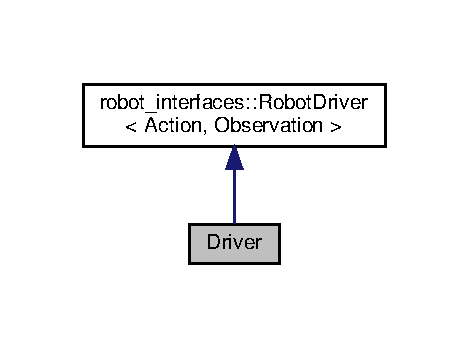
\includegraphics[width=225pt]{classDriver__inherit__graph}
\end{center}
\end{figure}


Collaboration diagram for Driver\+:
\nopagebreak
\begin{figure}[H]
\begin{center}
\leavevmode
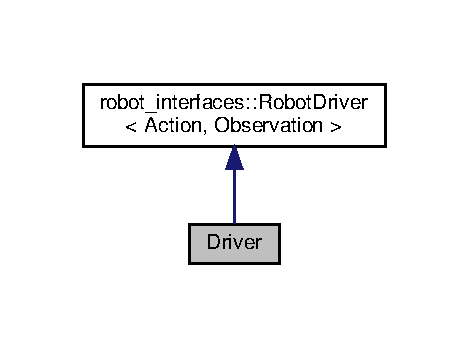
\includegraphics[width=225pt]{classDriver__coll__graph}
\end{center}
\end{figure}
\subsection*{Public Member Functions}
\begin{DoxyCompactItemize}
\item 
void \hyperlink{classDriver_a81c0beb523fad80cd40cfcc6a6e3de2d}{initialize} ()
\begin{DoxyCompactList}\small\item\em Initialize the robot. \end{DoxyCompactList}\item 
Action \hyperlink{classDriver_a0f8d51bef151ccc38a0cb7b226048e28}{apply\+\_\+action} (const Action \&action\+\_\+to\+\_\+apply)
\begin{DoxyCompactList}\small\item\em Apply action immediately and block until it is executed. \end{DoxyCompactList}\item 
Observation \hyperlink{classDriver_afb09663997bffc5c694fb5aa8aca243a}{get\+\_\+latest\+\_\+observation} ()
\begin{DoxyCompactList}\small\item\em Return the latest observation immediately. \end{DoxyCompactList}\item 
std\+::string \hyperlink{classDriver_a6fb739b87c892c4102e838508855c0be}{get\+\_\+error} ()
\begin{DoxyCompactList}\small\item\em Get error message if there is any error. \end{DoxyCompactList}\item 
void \hyperlink{classDriver_a630fc9183eb419beb09b5828b4547b6d}{shutdown} ()
\begin{DoxyCompactList}\small\item\em Shut down the robot safely. \end{DoxyCompactList}\end{DoxyCompactItemize}
\subsection*{Private Attributes}
\begin{DoxyCompactItemize}
\item 
\mbox{\Hypertarget{classDriver_acf6c56cd7c260695439a8625fa07aef9}\label{classDriver_acf6c56cd7c260695439a8625fa07aef9}} 
int {\bfseries state\+\_\+} \mbox{[}2\mbox{]}
\end{DoxyCompactItemize}
\subsection*{Static Private Attributes}
\begin{DoxyCompactItemize}
\item 
\mbox{\Hypertarget{classDriver_a2f75d16f4af650ca9cf1cdd8b653cc18}\label{classDriver_a2f75d16f4af650ca9cf1cdd8b653cc18}} 
static const int {\bfseries M\+AX} = 1000
\item 
\mbox{\Hypertarget{classDriver_a09b06e92e4ea9df756e3b6e038fa25f6}\label{classDriver_a09b06e92e4ea9df756e3b6e038fa25f6}} 
static const int {\bfseries M\+IN} = 0
\end{DoxyCompactItemize}
\subsection*{Additional Inherited Members}


\subsection{Detailed Description}
\begin{Desc}
\item[Examples\+: ]\par
\hyperlink{demo_multiprocess_backend_8cpp-example}{demo\+\_\+multiprocess\+\_\+backend.\+cpp}.\end{Desc}


\subsection{Member Function Documentation}
\mbox{\Hypertarget{classDriver_a0f8d51bef151ccc38a0cb7b226048e28}\label{classDriver_a0f8d51bef151ccc38a0cb7b226048e28}} 
\index{Driver@{Driver}!apply\+\_\+action@{apply\+\_\+action}}
\index{apply\+\_\+action@{apply\+\_\+action}!Driver@{Driver}}
\subsubsection{\texorpdfstring{apply\+\_\+action()}{apply\_action()}}
{\footnotesize\ttfamily Action Driver\+::apply\+\_\+action (\begin{DoxyParamCaption}\item[{const Action \&}]{desired\+\_\+action }\end{DoxyParamCaption})\hspace{0.3cm}{\ttfamily [inline]}, {\ttfamily [virtual]}}



Apply action immediately and block until it is executed. 

This method must apply the desired\+\_\+action immediately when it is called, and only return once the action has been executed completely. This way we can accommodate both simulators and real robots with this interface.


\begin{DoxyParams}{Parameters}
{\em desired\+\_\+action} & The action we want to apply. \\
\hline
\end{DoxyParams}
\begin{DoxyReturn}{Returns}
The action that was actually applied (since due to safety reasons it might not be possible to apply the desired action). 
\end{DoxyReturn}


Implements \hyperlink{classrobot__interfaces_1_1RobotDriver_a4294e522fcd12b38d69f7d53fae5d74a}{robot\+\_\+interfaces\+::\+Robot\+Driver$<$ Action, Observation $>$}.

\mbox{\Hypertarget{classDriver_a6fb739b87c892c4102e838508855c0be}\label{classDriver_a6fb739b87c892c4102e838508855c0be}} 
\index{Driver@{Driver}!get\+\_\+error@{get\+\_\+error}}
\index{get\+\_\+error@{get\+\_\+error}!Driver@{Driver}}
\subsubsection{\texorpdfstring{get\+\_\+error()}{get\_error()}}
{\footnotesize\ttfamily std\+::string Driver\+::get\+\_\+error (\begin{DoxyParamCaption}{ }\end{DoxyParamCaption})\hspace{0.3cm}{\ttfamily [inline]}, {\ttfamily [virtual]}}



Get error message if there is any error. 

\begin{DoxyReturn}{Returns}
Returns an error message or an empty string if there is no error. 
\end{DoxyReturn}


Implements \hyperlink{classrobot__interfaces_1_1RobotDriver_acdf4c5d6993b836a180e6b6fc12b3445}{robot\+\_\+interfaces\+::\+Robot\+Driver$<$ Action, Observation $>$}.

\mbox{\Hypertarget{classDriver_afb09663997bffc5c694fb5aa8aca243a}\label{classDriver_afb09663997bffc5c694fb5aa8aca243a}} 
\index{Driver@{Driver}!get\+\_\+latest\+\_\+observation@{get\+\_\+latest\+\_\+observation}}
\index{get\+\_\+latest\+\_\+observation@{get\+\_\+latest\+\_\+observation}!Driver@{Driver}}
\subsubsection{\texorpdfstring{get\+\_\+latest\+\_\+observation()}{get\_latest\_observation()}}
{\footnotesize\ttfamily Observation Driver\+::get\+\_\+latest\+\_\+observation (\begin{DoxyParamCaption}{ }\end{DoxyParamCaption})\hspace{0.3cm}{\ttfamily [inline]}, {\ttfamily [virtual]}}



Return the latest observation immediately. 

\begin{DoxyReturn}{Returns}
Observation 
\end{DoxyReturn}


Implements \hyperlink{classrobot__interfaces_1_1RobotDriver_ad13d4f4fdfe78bdde4fc964f07fa45e2}{robot\+\_\+interfaces\+::\+Robot\+Driver$<$ Action, Observation $>$}.

\mbox{\Hypertarget{classDriver_a81c0beb523fad80cd40cfcc6a6e3de2d}\label{classDriver_a81c0beb523fad80cd40cfcc6a6e3de2d}} 
\index{Driver@{Driver}!initialize@{initialize}}
\index{initialize@{initialize}!Driver@{Driver}}
\subsubsection{\texorpdfstring{initialize()}{initialize()}}
{\footnotesize\ttfamily void Driver\+::initialize (\begin{DoxyParamCaption}{ }\end{DoxyParamCaption})\hspace{0.3cm}{\ttfamily [inline]}, {\ttfamily [virtual]}}



Initialize the robot. 

Any initialization procedures that need to be done before sending actions to the robot should be done in this method (e.\+g. homing to find the absolute position). 

Implements \hyperlink{classrobot__interfaces_1_1RobotDriver_af3cbef570a455e1f8085d701282264ff}{robot\+\_\+interfaces\+::\+Robot\+Driver$<$ Action, Observation $>$}.

\mbox{\Hypertarget{classDriver_a630fc9183eb419beb09b5828b4547b6d}\label{classDriver_a630fc9183eb419beb09b5828b4547b6d}} 
\index{Driver@{Driver}!shutdown@{shutdown}}
\index{shutdown@{shutdown}!Driver@{Driver}}
\subsubsection{\texorpdfstring{shutdown()}{shutdown()}}
{\footnotesize\ttfamily void Driver\+::shutdown (\begin{DoxyParamCaption}{ }\end{DoxyParamCaption})\hspace{0.3cm}{\ttfamily [inline]}, {\ttfamily [virtual]}}



Shut down the robot safely. 

Use this method if your robot needs to perform some action when shutting down, e.\+g. to move it to a defined rest position. 

Implements \hyperlink{classrobot__interfaces_1_1RobotDriver_a3451fb8b15d2840b559f3ee858de01f8}{robot\+\_\+interfaces\+::\+Robot\+Driver$<$ Action, Observation $>$}.



The documentation for this class was generated from the following file\+:\begin{DoxyCompactItemize}
\item 
demos/\hyperlink{demo__multiprocess__backend_8cpp}{demo\+\_\+multiprocess\+\_\+backend.\+cpp}\end{DoxyCompactItemize}

\hypertarget{classrobot__interfaces_1_1example_1_1Driver}{}\section{robot\+\_\+interfaces\+:\+:example\+:\+:Driver Class Reference}
\label{classrobot__interfaces_1_1example_1_1Driver}\index{robot\+\_\+interfaces\+::example\+::\+Driver@{robot\+\_\+interfaces\+::example\+::\+Driver}}


Example \hyperlink{classrobot__interfaces_1_1Robot}{Robot} \hyperlink{classrobot__interfaces_1_1example_1_1Driver}{Driver}.  




{\ttfamily \#include $<$example.\+hpp$>$}



Inheritance diagram for robot\+\_\+interfaces\+:\+:example\+:\+:Driver\+:
\nopagebreak
\begin{figure}[H]
\begin{center}
\leavevmode
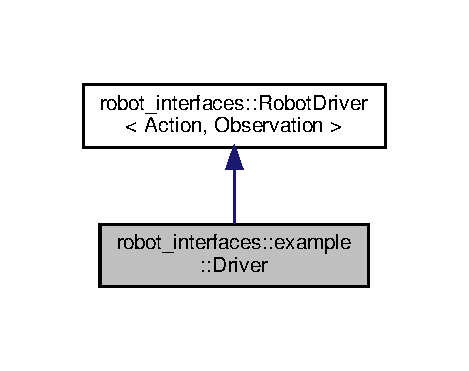
\includegraphics[width=225pt]{classrobot__interfaces_1_1example_1_1Driver__inherit__graph}
\end{center}
\end{figure}


Collaboration diagram for robot\+\_\+interfaces\+:\+:example\+:\+:Driver\+:
\nopagebreak
\begin{figure}[H]
\begin{center}
\leavevmode
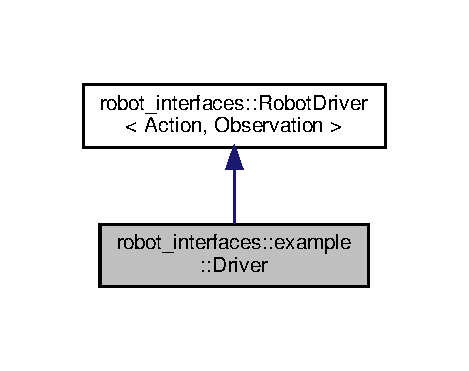
\includegraphics[width=225pt]{classrobot__interfaces_1_1example_1_1Driver__coll__graph}
\end{center}
\end{figure}
\subsection*{Public Member Functions}
\begin{DoxyCompactItemize}
\item 
\mbox{\Hypertarget{classrobot__interfaces_1_1example_1_1Driver_a83743c88f8873685b3b628e393ffe9fe}\label{classrobot__interfaces_1_1example_1_1Driver_a83743c88f8873685b3b628e393ffe9fe}} 
{\bfseries Driver} (int min, int max)
\item 
void \hyperlink{classrobot__interfaces_1_1example_1_1Driver_ab6f6c3f3ffb730d162bec70313f8aab7}{initialize} ()
\begin{DoxyCompactList}\small\item\em Initialize the robot. \end{DoxyCompactList}\item 
Action \hyperlink{classrobot__interfaces_1_1example_1_1Driver_aa18b1bc90441395e86794a90dfdac9fa}{apply\+\_\+action} (const Action \&action\+\_\+to\+\_\+apply)
\begin{DoxyCompactList}\small\item\em Apply action immediately and block until it is executed. \end{DoxyCompactList}\item 
Observation \hyperlink{classrobot__interfaces_1_1example_1_1Driver_a2fa7ee03258e65037ed69d9a8363bfe8}{get\+\_\+latest\+\_\+observation} ()
\begin{DoxyCompactList}\small\item\em Return the latest observation immediately. \end{DoxyCompactList}\item 
std\+::string \hyperlink{classrobot__interfaces_1_1example_1_1Driver_a8465b912da8f11a6db271f11ff4eced1}{get\+\_\+error} ()
\begin{DoxyCompactList}\small\item\em Get error message if there is any error. \end{DoxyCompactList}\item 
void \hyperlink{classrobot__interfaces_1_1example_1_1Driver_a91cbe74896c9ed56ff7eee6380964dfe}{shutdown} ()
\begin{DoxyCompactList}\small\item\em Shut down the robot safely. \end{DoxyCompactList}\end{DoxyCompactItemize}
\subsection*{Private Attributes}
\begin{DoxyCompactItemize}
\item 
\mbox{\Hypertarget{classrobot__interfaces_1_1example_1_1Driver_a86c0ec3574adbdb190ee17c51068b59a}\label{classrobot__interfaces_1_1example_1_1Driver_a86c0ec3574adbdb190ee17c51068b59a}} 
int {\bfseries state\+\_\+} \mbox{[}2\mbox{]}
\item 
\mbox{\Hypertarget{classrobot__interfaces_1_1example_1_1Driver_a6ffdfed257b3b4466615ec9d4cd7c2d1}\label{classrobot__interfaces_1_1example_1_1Driver_a6ffdfed257b3b4466615ec9d4cd7c2d1}} 
int {\bfseries min\+\_\+}
\item 
\mbox{\Hypertarget{classrobot__interfaces_1_1example_1_1Driver_a3d788870eb3c8043e0f3e278a11b87f6}\label{classrobot__interfaces_1_1example_1_1Driver_a3d788870eb3c8043e0f3e278a11b87f6}} 
int {\bfseries max\+\_\+}
\end{DoxyCompactItemize}
\subsection*{Additional Inherited Members}


\subsection{Detailed Description}
Example \hyperlink{classrobot__interfaces_1_1Robot}{Robot} \hyperlink{classrobot__interfaces_1_1example_1_1Driver}{Driver}. 

Send command to the robot and read observation from the robot. The D\+OF positions simply becomes the ones set by the latest action, capped between a min and a max value. 

\subsection{Member Function Documentation}
\mbox{\Hypertarget{classrobot__interfaces_1_1example_1_1Driver_aa18b1bc90441395e86794a90dfdac9fa}\label{classrobot__interfaces_1_1example_1_1Driver_aa18b1bc90441395e86794a90dfdac9fa}} 
\index{robot\+\_\+interfaces\+::example\+::\+Driver@{robot\+\_\+interfaces\+::example\+::\+Driver}!apply\+\_\+action@{apply\+\_\+action}}
\index{apply\+\_\+action@{apply\+\_\+action}!robot\+\_\+interfaces\+::example\+::\+Driver@{robot\+\_\+interfaces\+::example\+::\+Driver}}
\subsubsection{\texorpdfstring{apply\+\_\+action()}{apply\_action()}}
{\footnotesize\ttfamily Action robot\+\_\+interfaces\+::example\+::\+Driver\+::apply\+\_\+action (\begin{DoxyParamCaption}\item[{const Action \&}]{desired\+\_\+action }\end{DoxyParamCaption})\hspace{0.3cm}{\ttfamily [inline]}, {\ttfamily [virtual]}}



Apply action immediately and block until it is executed. 

This method must apply the desired\+\_\+action immediately when it is called, and only return once the action has been executed completely. This way we can accommodate both simulators and real robots with this interface.


\begin{DoxyParams}{Parameters}
{\em desired\+\_\+action} & The action we want to apply. \\
\hline
\end{DoxyParams}
\begin{DoxyReturn}{Returns}
The action that was actually applied (since due to safety reasons it might not be possible to apply the desired action). 
\end{DoxyReturn}


Implements \hyperlink{classrobot__interfaces_1_1RobotDriver_a4294e522fcd12b38d69f7d53fae5d74a}{robot\+\_\+interfaces\+::\+Robot\+Driver$<$ Action, Observation $>$}.

\mbox{\Hypertarget{classrobot__interfaces_1_1example_1_1Driver_a8465b912da8f11a6db271f11ff4eced1}\label{classrobot__interfaces_1_1example_1_1Driver_a8465b912da8f11a6db271f11ff4eced1}} 
\index{robot\+\_\+interfaces\+::example\+::\+Driver@{robot\+\_\+interfaces\+::example\+::\+Driver}!get\+\_\+error@{get\+\_\+error}}
\index{get\+\_\+error@{get\+\_\+error}!robot\+\_\+interfaces\+::example\+::\+Driver@{robot\+\_\+interfaces\+::example\+::\+Driver}}
\subsubsection{\texorpdfstring{get\+\_\+error()}{get\_error()}}
{\footnotesize\ttfamily std\+::string robot\+\_\+interfaces\+::example\+::\+Driver\+::get\+\_\+error (\begin{DoxyParamCaption}{ }\end{DoxyParamCaption})\hspace{0.3cm}{\ttfamily [inline]}, {\ttfamily [virtual]}}



Get error message if there is any error. 

\begin{DoxyReturn}{Returns}
Returns an error message or an empty string if there is no error. 
\end{DoxyReturn}


Implements \hyperlink{classrobot__interfaces_1_1RobotDriver_acdf4c5d6993b836a180e6b6fc12b3445}{robot\+\_\+interfaces\+::\+Robot\+Driver$<$ Action, Observation $>$}.

\mbox{\Hypertarget{classrobot__interfaces_1_1example_1_1Driver_a2fa7ee03258e65037ed69d9a8363bfe8}\label{classrobot__interfaces_1_1example_1_1Driver_a2fa7ee03258e65037ed69d9a8363bfe8}} 
\index{robot\+\_\+interfaces\+::example\+::\+Driver@{robot\+\_\+interfaces\+::example\+::\+Driver}!get\+\_\+latest\+\_\+observation@{get\+\_\+latest\+\_\+observation}}
\index{get\+\_\+latest\+\_\+observation@{get\+\_\+latest\+\_\+observation}!robot\+\_\+interfaces\+::example\+::\+Driver@{robot\+\_\+interfaces\+::example\+::\+Driver}}
\subsubsection{\texorpdfstring{get\+\_\+latest\+\_\+observation()}{get\_latest\_observation()}}
{\footnotesize\ttfamily Observation robot\+\_\+interfaces\+::example\+::\+Driver\+::get\+\_\+latest\+\_\+observation (\begin{DoxyParamCaption}{ }\end{DoxyParamCaption})\hspace{0.3cm}{\ttfamily [inline]}, {\ttfamily [virtual]}}



Return the latest observation immediately. 

\begin{DoxyReturn}{Returns}
\hyperlink{classrobot__interfaces_1_1example_1_1Observation}{Observation} 
\end{DoxyReturn}


Implements \hyperlink{classrobot__interfaces_1_1RobotDriver_ad13d4f4fdfe78bdde4fc964f07fa45e2}{robot\+\_\+interfaces\+::\+Robot\+Driver$<$ Action, Observation $>$}.

\mbox{\Hypertarget{classrobot__interfaces_1_1example_1_1Driver_ab6f6c3f3ffb730d162bec70313f8aab7}\label{classrobot__interfaces_1_1example_1_1Driver_ab6f6c3f3ffb730d162bec70313f8aab7}} 
\index{robot\+\_\+interfaces\+::example\+::\+Driver@{robot\+\_\+interfaces\+::example\+::\+Driver}!initialize@{initialize}}
\index{initialize@{initialize}!robot\+\_\+interfaces\+::example\+::\+Driver@{robot\+\_\+interfaces\+::example\+::\+Driver}}
\subsubsection{\texorpdfstring{initialize()}{initialize()}}
{\footnotesize\ttfamily void robot\+\_\+interfaces\+::example\+::\+Driver\+::initialize (\begin{DoxyParamCaption}{ }\end{DoxyParamCaption})\hspace{0.3cm}{\ttfamily [inline]}, {\ttfamily [virtual]}}



Initialize the robot. 

Any initialization procedures that need to be done before sending actions to the robot should be done in this method (e.\+g. homing to find the absolute position). 

Implements \hyperlink{classrobot__interfaces_1_1RobotDriver_af3cbef570a455e1f8085d701282264ff}{robot\+\_\+interfaces\+::\+Robot\+Driver$<$ Action, Observation $>$}.

\mbox{\Hypertarget{classrobot__interfaces_1_1example_1_1Driver_a91cbe74896c9ed56ff7eee6380964dfe}\label{classrobot__interfaces_1_1example_1_1Driver_a91cbe74896c9ed56ff7eee6380964dfe}} 
\index{robot\+\_\+interfaces\+::example\+::\+Driver@{robot\+\_\+interfaces\+::example\+::\+Driver}!shutdown@{shutdown}}
\index{shutdown@{shutdown}!robot\+\_\+interfaces\+::example\+::\+Driver@{robot\+\_\+interfaces\+::example\+::\+Driver}}
\subsubsection{\texorpdfstring{shutdown()}{shutdown()}}
{\footnotesize\ttfamily void robot\+\_\+interfaces\+::example\+::\+Driver\+::shutdown (\begin{DoxyParamCaption}{ }\end{DoxyParamCaption})\hspace{0.3cm}{\ttfamily [inline]}, {\ttfamily [virtual]}}



Shut down the robot safely. 

Use this method if your robot needs to perform some action when shutting down, e.\+g. to move it to a defined rest position. 

Implements \hyperlink{classrobot__interfaces_1_1RobotDriver_a3451fb8b15d2840b559f3ee858de01f8}{robot\+\_\+interfaces\+::\+Robot\+Driver$<$ Action, Observation $>$}.



The documentation for this class was generated from the following file\+:\begin{DoxyCompactItemize}
\item 
include/robot\+\_\+interfaces/\hyperlink{example_8hpp}{example.\+hpp}\end{DoxyCompactItemize}

\hypertarget{structrobot__interfaces_1_1FingerTypes}{}\section{robot\+\_\+interfaces\+:\+:Finger\+Types$<$ N\+\_\+\+F\+I\+N\+G\+E\+RS $>$ Struct Template Reference}
\label{structrobot__interfaces_1_1FingerTypes}\index{robot\+\_\+interfaces\+::\+Finger\+Types$<$ N\+\_\+\+F\+I\+N\+G\+E\+R\+S $>$@{robot\+\_\+interfaces\+::\+Finger\+Types$<$ N\+\_\+\+F\+I\+N\+G\+E\+R\+S $>$}}


Types for the Finger robot (basic 3-\/joint robot).  




{\ttfamily \#include $<$finger\+\_\+types.\+hpp$>$}



Inheritance diagram for robot\+\_\+interfaces\+:\+:Finger\+Types$<$ N\+\_\+\+F\+I\+N\+G\+E\+RS $>$\+:
\nopagebreak
\begin{figure}[H]
\begin{center}
\leavevmode
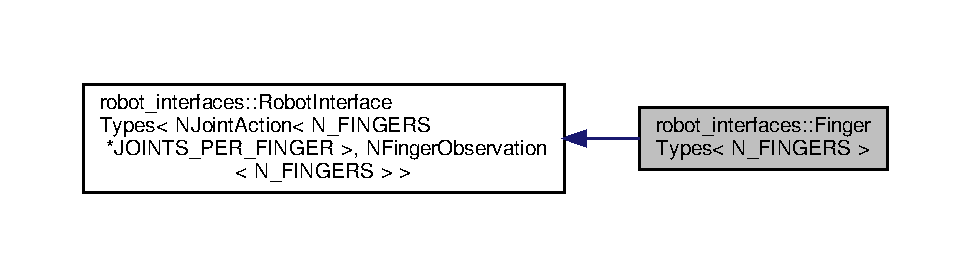
\includegraphics[width=350pt]{structrobot__interfaces_1_1FingerTypes__inherit__graph}
\end{center}
\end{figure}


Collaboration diagram for robot\+\_\+interfaces\+:\+:Finger\+Types$<$ N\+\_\+\+F\+I\+N\+G\+E\+RS $>$\+:
\nopagebreak
\begin{figure}[H]
\begin{center}
\leavevmode
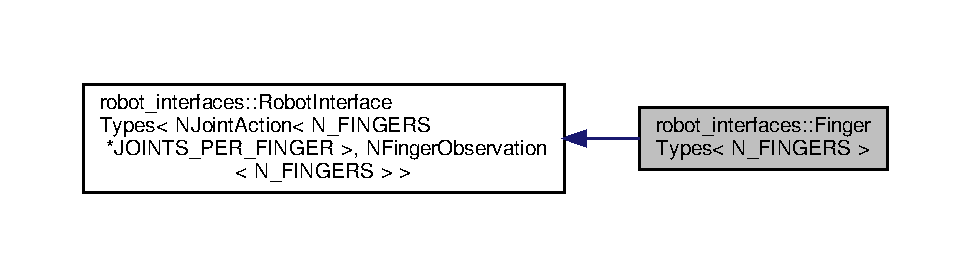
\includegraphics[width=350pt]{structrobot__interfaces_1_1FingerTypes__coll__graph}
\end{center}
\end{figure}
\subsection*{Additional Inherited Members}


\subsection{Detailed Description}
\subsubsection*{template$<$size\+\_\+t N\+\_\+\+F\+I\+N\+G\+E\+RS$>$\newline
struct robot\+\_\+interfaces\+::\+Finger\+Types$<$ N\+\_\+\+F\+I\+N\+G\+E\+R\+S $>$}

Types for the Finger robot (basic 3-\/joint robot). 

The documentation for this struct was generated from the following file\+:\begin{DoxyCompactItemize}
\item 
include/robot\+\_\+interfaces/finger\+\_\+types.\+hpp\end{DoxyCompactItemize}

\hypertarget{classrobot__interfaces_1_1Loggable}{}\section{robot\+\_\+interfaces\+:\+:Loggable Class Reference}
\label{classrobot__interfaces_1_1Loggable}\index{robot\+\_\+interfaces\+::\+Loggable@{robot\+\_\+interfaces\+::\+Loggable}}


Inheritance diagram for robot\+\_\+interfaces\+:\+:Loggable\+:
\nopagebreak
\begin{figure}[H]
\begin{center}
\leavevmode
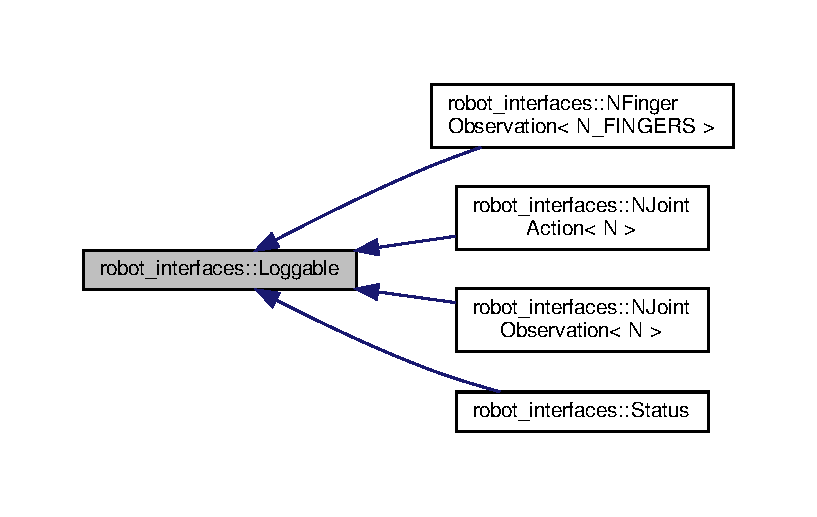
\includegraphics[width=350pt]{classrobot__interfaces_1_1Loggable__inherit__graph}
\end{center}
\end{figure}
\subsection*{Public Member Functions}
\begin{DoxyCompactItemize}
\item 
\mbox{\Hypertarget{classrobot__interfaces_1_1Loggable_a19635ebc166379f11fe4c8e58153243a}\label{classrobot__interfaces_1_1Loggable_a19635ebc166379f11fe4c8e58153243a}} 
virtual std\+::vector$<$ std\+::string $>$ {\bfseries get\+\_\+name} ()=0
\item 
\mbox{\Hypertarget{classrobot__interfaces_1_1Loggable_a28ffee45cf66a84d16b2c907ed10367c}\label{classrobot__interfaces_1_1Loggable_a28ffee45cf66a84d16b2c907ed10367c}} 
virtual std\+::vector$<$ std\+::vector$<$ double $>$ $>$ {\bfseries get\+\_\+data} ()=0
\end{DoxyCompactItemize}


The documentation for this class was generated from the following file\+:\begin{DoxyCompactItemize}
\item 
include/robot\+\_\+interfaces/loggable.\+hpp\end{DoxyCompactItemize}

\hypertarget{classrobot__interfaces_1_1MonitoredRobotDriver}{}\section{robot\+\_\+interfaces\+:\+:Monitored\+Robot\+Driver$<$ Driver $>$ Class Template Reference}
\label{classrobot__interfaces_1_1MonitoredRobotDriver}\index{robot\+\_\+interfaces\+::\+Monitored\+Robot\+Driver$<$ Driver $>$@{robot\+\_\+interfaces\+::\+Monitored\+Robot\+Driver$<$ Driver $>$}}


Wrapper for \hyperlink{classrobot__interfaces_1_1RobotDriver}{Robot\+Driver} that monitors timing.  




{\ttfamily \#include $<$monitored\+\_\+robot\+\_\+driver.\+hpp$>$}



Inheritance diagram for robot\+\_\+interfaces\+:\+:Monitored\+Robot\+Driver$<$ Driver $>$\+:
\nopagebreak
\begin{figure}[H]
\begin{center}
\leavevmode
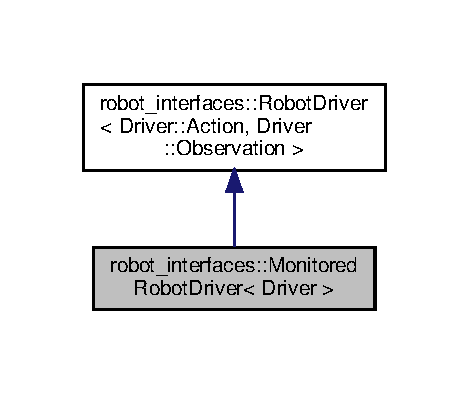
\includegraphics[width=225pt]{classrobot__interfaces_1_1MonitoredRobotDriver__inherit__graph}
\end{center}
\end{figure}


Collaboration diagram for robot\+\_\+interfaces\+:\+:Monitored\+Robot\+Driver$<$ Driver $>$\+:
\nopagebreak
\begin{figure}[H]
\begin{center}
\leavevmode
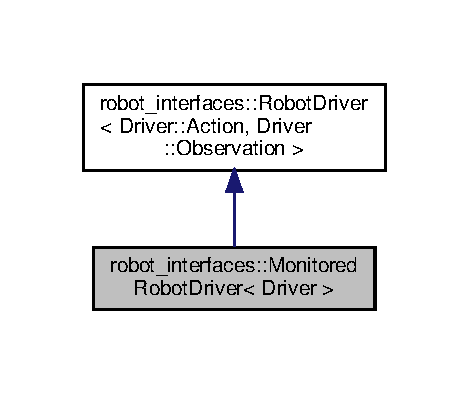
\includegraphics[width=225pt]{classrobot__interfaces_1_1MonitoredRobotDriver__coll__graph}
\end{center}
\end{figure}
\subsection*{Public Types}
\begin{DoxyCompactItemize}
\item 
\mbox{\Hypertarget{classrobot__interfaces_1_1MonitoredRobotDriver_a272fbf2c9bf93f568c00dd1e37e62e97}\label{classrobot__interfaces_1_1MonitoredRobotDriver_a272fbf2c9bf93f568c00dd1e37e62e97}} 
typedef std\+::shared\+\_\+ptr$<$ \hyperlink{classDriver}{Driver} $>$ {\bfseries Robot\+Driver\+Ptr}
\end{DoxyCompactItemize}
\subsection*{Public Member Functions}
\begin{DoxyCompactItemize}
\item 
\hyperlink{classrobot__interfaces_1_1MonitoredRobotDriver_a2ea1456e85ad7596295cb047e552dc06}{Monitored\+Robot\+Driver} (Robot\+Driver\+Ptr robot\+\_\+driver, const double max\+\_\+action\+\_\+duration\+\_\+s, const double max\+\_\+inter\+\_\+action\+\_\+duration\+\_\+s)
\begin{DoxyCompactList}\small\item\em Starts a thread for monitoring timing of action execution. \end{DoxyCompactList}\item 
\mbox{\Hypertarget{classrobot__interfaces_1_1MonitoredRobotDriver_a07dfd2cc6f1dc07fad82914814a43188}\label{classrobot__interfaces_1_1MonitoredRobotDriver_a07dfd2cc6f1dc07fad82914814a43188}} 
\hyperlink{classrobot__interfaces_1_1MonitoredRobotDriver_a07dfd2cc6f1dc07fad82914814a43188}{$\sim$\+Monitored\+Robot\+Driver} ()
\begin{DoxyCompactList}\small\item\em Shuts down the robot and stops the monitoring thread. \end{DoxyCompactList}\item 
virtual Driver\+::\+Action \hyperlink{classrobot__interfaces_1_1MonitoredRobotDriver_a3f0f7cbf74236e91d33dcfc08206b5e9}{apply\+\_\+action} (const typename Driver\+::\+Action \&desired\+\_\+action) final
\begin{DoxyCompactList}\small\item\em Apply desired action on the robot. \end{DoxyCompactList}\item 
virtual void \hyperlink{classrobot__interfaces_1_1MonitoredRobotDriver_a47b68c24afaa087e4e60e6413ab7ac89}{initialize} ()
\begin{DoxyCompactList}\small\item\em Initialize the robot. \end{DoxyCompactList}\item 
virtual Driver\+::\+Observation \hyperlink{classrobot__interfaces_1_1MonitoredRobotDriver_a97774dddcda1038f338d18ef0b572ad8}{get\+\_\+latest\+\_\+observation} ()
\begin{DoxyCompactList}\small\item\em Return the latest observation immediately. \end{DoxyCompactList}\item 
virtual std\+::string \hyperlink{classrobot__interfaces_1_1MonitoredRobotDriver_a944425cc7e0845184f33b16405a9e61e}{get\+\_\+error} ()
\begin{DoxyCompactList}\small\item\em Get error message if there is any error. \end{DoxyCompactList}\item 
virtual void \hyperlink{classrobot__interfaces_1_1MonitoredRobotDriver_a95714a60e69a3ac06461382a7b391289}{shutdown} () final
\begin{DoxyCompactList}\small\item\em Shut down the robot safely. \end{DoxyCompactList}\end{DoxyCompactItemize}
\subsection*{Private Member Functions}
\begin{DoxyCompactItemize}
\item 
void \hyperlink{classrobot__interfaces_1_1MonitoredRobotDriver_a6ed3d940dce484dcdc558a52a8dfe8a5}{loop} ()
\begin{DoxyCompactList}\small\item\em Monitor the timing of action execution. \end{DoxyCompactList}\end{DoxyCompactItemize}
\subsection*{Static Private Member Functions}
\begin{DoxyCompactItemize}
\item 
\mbox{\Hypertarget{classrobot__interfaces_1_1MonitoredRobotDriver_a46ddb0472196631d6cdd109f3753c693}\label{classrobot__interfaces_1_1MonitoredRobotDriver_a46ddb0472196631d6cdd109f3753c693}} 
static void $\ast$ {\bfseries loop} (void $\ast$instance\+\_\+pointer)
\end{DoxyCompactItemize}
\subsection*{Private Attributes}
\begin{DoxyCompactItemize}
\item 
\mbox{\Hypertarget{classrobot__interfaces_1_1MonitoredRobotDriver_ae43540d38c9414d8ad734a9c88155a6e}\label{classrobot__interfaces_1_1MonitoredRobotDriver_ae43540d38c9414d8ad734a9c88155a6e}} 
Robot\+Driver\+Ptr \hyperlink{classrobot__interfaces_1_1MonitoredRobotDriver_ae43540d38c9414d8ad734a9c88155a6e}{robot\+\_\+driver\+\_\+}
\begin{DoxyCompactList}\small\item\em The actual robot driver. \end{DoxyCompactList}\item 
\mbox{\Hypertarget{classrobot__interfaces_1_1MonitoredRobotDriver_a860e5a4835a916faf08e1ab932b34bb1}\label{classrobot__interfaces_1_1MonitoredRobotDriver_a860e5a4835a916faf08e1ab932b34bb1}} 
double \hyperlink{classrobot__interfaces_1_1MonitoredRobotDriver_a860e5a4835a916faf08e1ab932b34bb1}{max\+\_\+action\+\_\+duration\+\_\+s\+\_\+}
\begin{DoxyCompactList}\small\item\em Max. time for executing an action. \end{DoxyCompactList}\item 
\mbox{\Hypertarget{classrobot__interfaces_1_1MonitoredRobotDriver_acef35c51b51f1d05453b5b672f43a516}\label{classrobot__interfaces_1_1MonitoredRobotDriver_acef35c51b51f1d05453b5b672f43a516}} 
double \hyperlink{classrobot__interfaces_1_1MonitoredRobotDriver_acef35c51b51f1d05453b5b672f43a516}{max\+\_\+inter\+\_\+action\+\_\+duration\+\_\+s\+\_\+}
\begin{DoxyCompactList}\small\item\em Max. idle time between actions. \end{DoxyCompactList}\item 
\mbox{\Hypertarget{classrobot__interfaces_1_1MonitoredRobotDriver_a8200e14e4d9e4d1d8c2fc4e0134cf7cd}\label{classrobot__interfaces_1_1MonitoredRobotDriver_a8200e14e4d9e4d1d8c2fc4e0134cf7cd}} 
std\+::atomic$<$ bool $>$ \hyperlink{classrobot__interfaces_1_1MonitoredRobotDriver_a8200e14e4d9e4d1d8c2fc4e0134cf7cd}{is\+\_\+shutdown\+\_\+}
\begin{DoxyCompactList}\small\item\em Whether shutdown was initiated. \end{DoxyCompactList}\item 
\mbox{\Hypertarget{classrobot__interfaces_1_1MonitoredRobotDriver_a5c02465be067a76143495c47469d0ae3}\label{classrobot__interfaces_1_1MonitoredRobotDriver_a5c02465be067a76143495c47469d0ae3}} 
time\+\_\+series\+::\+Time\+Series$<$ bool $>$ {\bfseries action\+\_\+start\+\_\+logger\+\_\+}
\item 
\mbox{\Hypertarget{classrobot__interfaces_1_1MonitoredRobotDriver_a469ee1c7ec3565e391c9ac1758b702f6}\label{classrobot__interfaces_1_1MonitoredRobotDriver_a469ee1c7ec3565e391c9ac1758b702f6}} 
time\+\_\+series\+::\+Time\+Series$<$ bool $>$ {\bfseries action\+\_\+end\+\_\+logger\+\_\+}
\item 
\mbox{\Hypertarget{classrobot__interfaces_1_1MonitoredRobotDriver_aaa3c0cd73914d3d3118a78252ed13631}\label{classrobot__interfaces_1_1MonitoredRobotDriver_aaa3c0cd73914d3d3118a78252ed13631}} 
std\+::shared\+\_\+ptr$<$ real\+\_\+time\+\_\+tools\+::\+Real\+Time\+Thread $>$ {\bfseries thread\+\_\+}
\item 
\mbox{\Hypertarget{classrobot__interfaces_1_1MonitoredRobotDriver_a123c65db418751fccfd681e0cc53348a}\label{classrobot__interfaces_1_1MonitoredRobotDriver_a123c65db418751fccfd681e0cc53348a}} 
real\+\_\+time\+\_\+tools\+::\+Singletype\+Threadsafe\+Object$<$ std\+::string, 1 $>$ {\bfseries error\+\_\+message\+\_\+}
\end{DoxyCompactItemize}


\subsection{Detailed Description}
\subsubsection*{template$<$typename Driver$>$\newline
class robot\+\_\+interfaces\+::\+Monitored\+Robot\+Driver$<$ Driver $>$}

Wrapper for \hyperlink{classrobot__interfaces_1_1RobotDriver}{Robot\+Driver} that monitors timing. 

Takes a \hyperlink{classrobot__interfaces_1_1RobotDriver}{Robot\+Driver} instance as input and forwards all method calls to it. A background loop monitors timing of actions to ensure the following constraints\+:


\begin{DoxyEnumerate}
\item The execution of an action does not take longer than {\ttfamily max\+\_\+action\+\_\+duration\+\_\+s\+\_\+} seconds.
\item The time interval between termination of the previous action and receival of the next one (through {\ttfamily \hyperlink{classrobot__interfaces_1_1MonitoredRobotDriver_a3f0f7cbf74236e91d33dcfc08206b5e9}{apply\+\_\+action()}}) does not exceed {\ttfamily max\+\_\+inter\+\_\+action\+\_\+duration\+\_\+s\+\_\+}.
\end{DoxyEnumerate}

If these timing constraints are not satisfied, the robot will be shutdown, and no more actions from the outside will be accepted.

This wrapper also makes sure that the {\ttfamily \hyperlink{classrobot__interfaces_1_1MonitoredRobotDriver_a95714a60e69a3ac06461382a7b391289}{shutdown()}} method of the given \hyperlink{classrobot__interfaces_1_1RobotDriver}{Robot\+Driver} is called when wrapper is destroyed, so the robot should always be left in a safe state.


\begin{DoxyTemplParams}{Template Parameters}
{\em Action} & \\
\hline
{\em Observation} & \\
\hline
\end{DoxyTemplParams}


\subsection{Constructor \& Destructor Documentation}
\mbox{\Hypertarget{classrobot__interfaces_1_1MonitoredRobotDriver_a2ea1456e85ad7596295cb047e552dc06}\label{classrobot__interfaces_1_1MonitoredRobotDriver_a2ea1456e85ad7596295cb047e552dc06}} 
\index{robot\+\_\+interfaces\+::\+Monitored\+Robot\+Driver@{robot\+\_\+interfaces\+::\+Monitored\+Robot\+Driver}!Monitored\+Robot\+Driver@{Monitored\+Robot\+Driver}}
\index{Monitored\+Robot\+Driver@{Monitored\+Robot\+Driver}!robot\+\_\+interfaces\+::\+Monitored\+Robot\+Driver@{robot\+\_\+interfaces\+::\+Monitored\+Robot\+Driver}}
\subsubsection{\texorpdfstring{Monitored\+Robot\+Driver()}{MonitoredRobotDriver()}}
{\footnotesize\ttfamily template$<$typename Driver $>$ \\
\hyperlink{classrobot__interfaces_1_1MonitoredRobotDriver}{robot\+\_\+interfaces\+::\+Monitored\+Robot\+Driver}$<$ \hyperlink{classDriver}{Driver} $>$\+::\hyperlink{classrobot__interfaces_1_1MonitoredRobotDriver}{Monitored\+Robot\+Driver} (\begin{DoxyParamCaption}\item[{Robot\+Driver\+Ptr}]{robot\+\_\+driver,  }\item[{const double}]{max\+\_\+action\+\_\+duration\+\_\+s,  }\item[{const double}]{max\+\_\+inter\+\_\+action\+\_\+duration\+\_\+s }\end{DoxyParamCaption})\hspace{0.3cm}{\ttfamily [inline]}}



Starts a thread for monitoring timing of action execution. 


\begin{DoxyParams}{Parameters}
{\em robot\+\_\+driver} & The actual robot driver instance. \\
\hline
{\em max\+\_\+action\+\_\+duration\+\_\+s} & Maximum time allowed for an action to be executed. \\
\hline
{\em max\+\_\+inter\+\_\+action\+\_\+duration\+\_\+s} & Maximum time allowed between end of the previous action and receival of the next one. \\
\hline
\end{DoxyParams}


\subsection{Member Function Documentation}
\mbox{\Hypertarget{classrobot__interfaces_1_1MonitoredRobotDriver_a3f0f7cbf74236e91d33dcfc08206b5e9}\label{classrobot__interfaces_1_1MonitoredRobotDriver_a3f0f7cbf74236e91d33dcfc08206b5e9}} 
\index{robot\+\_\+interfaces\+::\+Monitored\+Robot\+Driver@{robot\+\_\+interfaces\+::\+Monitored\+Robot\+Driver}!apply\+\_\+action@{apply\+\_\+action}}
\index{apply\+\_\+action@{apply\+\_\+action}!robot\+\_\+interfaces\+::\+Monitored\+Robot\+Driver@{robot\+\_\+interfaces\+::\+Monitored\+Robot\+Driver}}
\subsubsection{\texorpdfstring{apply\+\_\+action()}{apply\_action()}}
{\footnotesize\ttfamily template$<$typename Driver $>$ \\
virtual Driver\+::\+Action \hyperlink{classrobot__interfaces_1_1MonitoredRobotDriver}{robot\+\_\+interfaces\+::\+Monitored\+Robot\+Driver}$<$ \hyperlink{classDriver}{Driver} $>$\+::apply\+\_\+action (\begin{DoxyParamCaption}\item[{const typename Driver\+::\+Action \&}]{desired\+\_\+action }\end{DoxyParamCaption})\hspace{0.3cm}{\ttfamily [inline]}, {\ttfamily [final]}, {\ttfamily [virtual]}}



Apply desired action on the robot. 

If the robot is shut down, no more actions will be applied (the method will just ignore them silently.


\begin{DoxyParams}{Parameters}
{\em desired\+\_\+action} & The desired action. \\
\hline
\end{DoxyParams}
\begin{DoxyReturn}{Returns}
The action that is actually applied on the robot (may differ from desired action due to safety limitations). 
\end{DoxyReturn}
\mbox{\Hypertarget{classrobot__interfaces_1_1MonitoredRobotDriver_a944425cc7e0845184f33b16405a9e61e}\label{classrobot__interfaces_1_1MonitoredRobotDriver_a944425cc7e0845184f33b16405a9e61e}} 
\index{robot\+\_\+interfaces\+::\+Monitored\+Robot\+Driver@{robot\+\_\+interfaces\+::\+Monitored\+Robot\+Driver}!get\+\_\+error@{get\+\_\+error}}
\index{get\+\_\+error@{get\+\_\+error}!robot\+\_\+interfaces\+::\+Monitored\+Robot\+Driver@{robot\+\_\+interfaces\+::\+Monitored\+Robot\+Driver}}
\subsubsection{\texorpdfstring{get\+\_\+error()}{get\_error()}}
{\footnotesize\ttfamily template$<$typename Driver $>$ \\
virtual std\+::string \hyperlink{classrobot__interfaces_1_1MonitoredRobotDriver}{robot\+\_\+interfaces\+::\+Monitored\+Robot\+Driver}$<$ \hyperlink{classDriver}{Driver} $>$\+::get\+\_\+error (\begin{DoxyParamCaption}{ }\end{DoxyParamCaption})\hspace{0.3cm}{\ttfamily [inline]}, {\ttfamily [virtual]}}



Get error message if there is any error. 

\begin{DoxyReturn}{Returns}
Returns an error message or an empty string if there is no error. 
\end{DoxyReturn}


Implements \hyperlink{classrobot__interfaces_1_1RobotDriver_acdf4c5d6993b836a180e6b6fc12b3445}{robot\+\_\+interfaces\+::\+Robot\+Driver$<$ Driver\+::\+Action, Driver\+::\+Observation $>$}.

\mbox{\Hypertarget{classrobot__interfaces_1_1MonitoredRobotDriver_a97774dddcda1038f338d18ef0b572ad8}\label{classrobot__interfaces_1_1MonitoredRobotDriver_a97774dddcda1038f338d18ef0b572ad8}} 
\index{robot\+\_\+interfaces\+::\+Monitored\+Robot\+Driver@{robot\+\_\+interfaces\+::\+Monitored\+Robot\+Driver}!get\+\_\+latest\+\_\+observation@{get\+\_\+latest\+\_\+observation}}
\index{get\+\_\+latest\+\_\+observation@{get\+\_\+latest\+\_\+observation}!robot\+\_\+interfaces\+::\+Monitored\+Robot\+Driver@{robot\+\_\+interfaces\+::\+Monitored\+Robot\+Driver}}
\subsubsection{\texorpdfstring{get\+\_\+latest\+\_\+observation()}{get\_latest\_observation()}}
{\footnotesize\ttfamily template$<$typename Driver $>$ \\
virtual Driver\+::\+Observation \hyperlink{classrobot__interfaces_1_1MonitoredRobotDriver}{robot\+\_\+interfaces\+::\+Monitored\+Robot\+Driver}$<$ \hyperlink{classDriver}{Driver} $>$\+::get\+\_\+latest\+\_\+observation (\begin{DoxyParamCaption}{ }\end{DoxyParamCaption})\hspace{0.3cm}{\ttfamily [inline]}, {\ttfamily [virtual]}}



Return the latest observation immediately. 

\begin{DoxyReturn}{Returns}
Observation 
\end{DoxyReturn}


Implements \hyperlink{classrobot__interfaces_1_1RobotDriver_ad13d4f4fdfe78bdde4fc964f07fa45e2}{robot\+\_\+interfaces\+::\+Robot\+Driver$<$ Driver\+::\+Action, Driver\+::\+Observation $>$}.

\mbox{\Hypertarget{classrobot__interfaces_1_1MonitoredRobotDriver_a47b68c24afaa087e4e60e6413ab7ac89}\label{classrobot__interfaces_1_1MonitoredRobotDriver_a47b68c24afaa087e4e60e6413ab7ac89}} 
\index{robot\+\_\+interfaces\+::\+Monitored\+Robot\+Driver@{robot\+\_\+interfaces\+::\+Monitored\+Robot\+Driver}!initialize@{initialize}}
\index{initialize@{initialize}!robot\+\_\+interfaces\+::\+Monitored\+Robot\+Driver@{robot\+\_\+interfaces\+::\+Monitored\+Robot\+Driver}}
\subsubsection{\texorpdfstring{initialize()}{initialize()}}
{\footnotesize\ttfamily template$<$typename Driver $>$ \\
virtual void \hyperlink{classrobot__interfaces_1_1MonitoredRobotDriver}{robot\+\_\+interfaces\+::\+Monitored\+Robot\+Driver}$<$ \hyperlink{classDriver}{Driver} $>$\+::initialize (\begin{DoxyParamCaption}{ }\end{DoxyParamCaption})\hspace{0.3cm}{\ttfamily [inline]}, {\ttfamily [virtual]}}



Initialize the robot. 

Any initialization procedures that need to be done before sending actions to the robot should be done in this method (e.\+g. homing to find the absolute position). 

Implements \hyperlink{classrobot__interfaces_1_1RobotDriver_af3cbef570a455e1f8085d701282264ff}{robot\+\_\+interfaces\+::\+Robot\+Driver$<$ Driver\+::\+Action, Driver\+::\+Observation $>$}.

\mbox{\Hypertarget{classrobot__interfaces_1_1MonitoredRobotDriver_a6ed3d940dce484dcdc558a52a8dfe8a5}\label{classrobot__interfaces_1_1MonitoredRobotDriver_a6ed3d940dce484dcdc558a52a8dfe8a5}} 
\index{robot\+\_\+interfaces\+::\+Monitored\+Robot\+Driver@{robot\+\_\+interfaces\+::\+Monitored\+Robot\+Driver}!loop@{loop}}
\index{loop@{loop}!robot\+\_\+interfaces\+::\+Monitored\+Robot\+Driver@{robot\+\_\+interfaces\+::\+Monitored\+Robot\+Driver}}
\subsubsection{\texorpdfstring{loop()}{loop()}}
{\footnotesize\ttfamily template$<$typename Driver $>$ \\
void \hyperlink{classrobot__interfaces_1_1MonitoredRobotDriver}{robot\+\_\+interfaces\+::\+Monitored\+Robot\+Driver}$<$ \hyperlink{classDriver}{Driver} $>$\+::loop (\begin{DoxyParamCaption}{ }\end{DoxyParamCaption})\hspace{0.3cm}{\ttfamily [inline]}, {\ttfamily [private]}}



Monitor the timing of action execution. 

If one of the timing constrains is violated, the robot is immediately shut down. \mbox{\Hypertarget{classrobot__interfaces_1_1MonitoredRobotDriver_a95714a60e69a3ac06461382a7b391289}\label{classrobot__interfaces_1_1MonitoredRobotDriver_a95714a60e69a3ac06461382a7b391289}} 
\index{robot\+\_\+interfaces\+::\+Monitored\+Robot\+Driver@{robot\+\_\+interfaces\+::\+Monitored\+Robot\+Driver}!shutdown@{shutdown}}
\index{shutdown@{shutdown}!robot\+\_\+interfaces\+::\+Monitored\+Robot\+Driver@{robot\+\_\+interfaces\+::\+Monitored\+Robot\+Driver}}
\subsubsection{\texorpdfstring{shutdown()}{shutdown()}}
{\footnotesize\ttfamily template$<$typename Driver $>$ \\
virtual void \hyperlink{classrobot__interfaces_1_1MonitoredRobotDriver}{robot\+\_\+interfaces\+::\+Monitored\+Robot\+Driver}$<$ \hyperlink{classDriver}{Driver} $>$\+::shutdown (\begin{DoxyParamCaption}{ }\end{DoxyParamCaption})\hspace{0.3cm}{\ttfamily [inline]}, {\ttfamily [final]}, {\ttfamily [virtual]}}



Shut down the robot safely. 

After shutdown, actions sent by the user are ignored. 

Implements \hyperlink{classrobot__interfaces_1_1RobotDriver_a3451fb8b15d2840b559f3ee858de01f8}{robot\+\_\+interfaces\+::\+Robot\+Driver$<$ Driver\+::\+Action, Driver\+::\+Observation $>$}.



The documentation for this class was generated from the following file\+:\begin{DoxyCompactItemize}
\item 
include/robot\+\_\+interfaces/monitored\+\_\+robot\+\_\+driver.\+hpp\end{DoxyCompactItemize}

\hypertarget{classrobot__interfaces_1_1MultiProcessRobotData}{}\section{robot\+\_\+interfaces\+:\+:Multi\+Process\+Robot\+Data$<$ Action, Observation $>$ Class Template Reference}
\label{classrobot__interfaces_1_1MultiProcessRobotData}\index{robot\+\_\+interfaces\+::\+Multi\+Process\+Robot\+Data$<$ Action, Observation $>$@{robot\+\_\+interfaces\+::\+Multi\+Process\+Robot\+Data$<$ Action, Observation $>$}}


\hyperlink{classrobot__interfaces_1_1RobotData}{Robot\+Data} instance using multi process time series.  




{\ttfamily \#include $<$robot\+\_\+data.\+hpp$>$}



Inheritance diagram for robot\+\_\+interfaces\+:\+:Multi\+Process\+Robot\+Data$<$ Action, Observation $>$\+:
\nopagebreak
\begin{figure}[H]
\begin{center}
\leavevmode
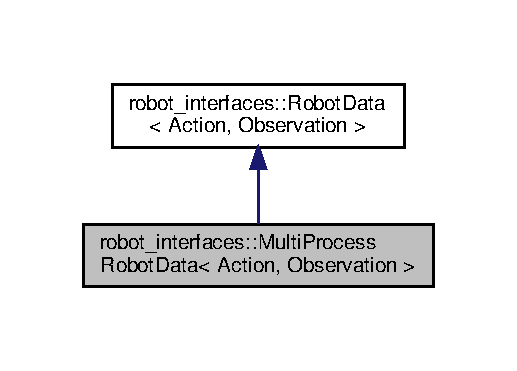
\includegraphics[width=248pt]{classrobot__interfaces_1_1MultiProcessRobotData__inherit__graph}
\end{center}
\end{figure}


Collaboration diagram for robot\+\_\+interfaces\+:\+:Multi\+Process\+Robot\+Data$<$ Action, Observation $>$\+:
\nopagebreak
\begin{figure}[H]
\begin{center}
\leavevmode
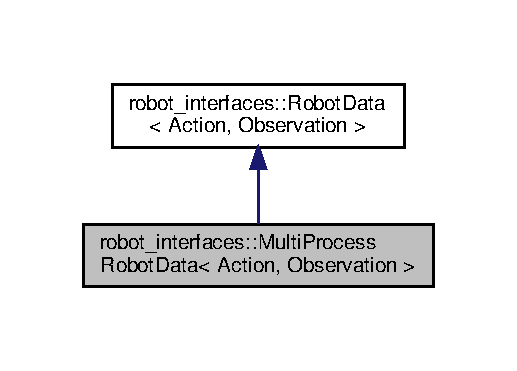
\includegraphics[width=248pt]{classrobot__interfaces_1_1MultiProcessRobotData__coll__graph}
\end{center}
\end{figure}
\subsection*{Public Member Functions}
\begin{DoxyCompactItemize}
\item 
\hyperlink{classrobot__interfaces_1_1MultiProcessRobotData_a27bb5ee187ceacb386d89c828481b057}{Multi\+Process\+Robot\+Data} (const std\+::string \&shared\+\_\+memory\+\_\+id\+\_\+prefix, bool is\+\_\+master, size\+\_\+t history\+\_\+length=1000)
\begin{DoxyCompactList}\small\item\em Construct the time series for the robot data. \end{DoxyCompactList}\end{DoxyCompactItemize}
\subsection*{Additional Inherited Members}


\subsection{Detailed Description}
\subsubsection*{template$<$typename Action, typename Observation$>$\newline
class robot\+\_\+interfaces\+::\+Multi\+Process\+Robot\+Data$<$ Action, Observation $>$}

\hyperlink{classrobot__interfaces_1_1RobotData}{Robot\+Data} instance using multi process time series. 

Use this class if modules accessing the data are running in separate processes. When all modules run as threads in the same process, this class can be used as well, however, \hyperlink{classrobot__interfaces_1_1SingleProcessRobotData}{Single\+Process\+Robot\+Data} might be more efficient in that case.

Contains all the input and output data of the robot. This means the
\begin{DoxyItemize}
\item {\ttfamily desired\+\_\+action} which was requested by the robot user
\item {\ttfamily applied\+\_\+action} which was actually applied and may not be and may not be identical to desired\+\_\+action for safety reasons
\item {\ttfamily observation} made by the robot
\item {\ttfamily status} which keeps track of timing issues and errors.
\end{DoxyItemize}

See this graph to understand how they relate to each other precisely in terms of time\+:

\begin{DoxyVerb}|------ t = 0 ------|------ t = 1 ------|
|----- action0 -----|----- action1 -----|
o                   o                   o
b                   b                   b
s                   s                   s
0                   1                   2
\end{DoxyVerb}



\begin{DoxyTemplParams}{Template Parameters}
{\em Action} & Type of the actions. \\
\hline
{\em Observation} & Type of the observations. \\
\hline
\end{DoxyTemplParams}
\begin{DoxySeeAlso}{See also}
\hyperlink{classrobot__interfaces_1_1SingleProcessRobotData}{Single\+Process\+Robot\+Data} 
\end{DoxySeeAlso}
\begin{Desc}
\item[Examples\+: ]\par
\hyperlink{demo_multiprocess_backend_8cpp-example}{demo\+\_\+multiprocess\+\_\+backend.\+cpp}, and \hyperlink{demo_multiprocess_frontend_8cpp-example}{demo\+\_\+multiprocess\+\_\+frontend.\+cpp}.\end{Desc}


\subsection{Constructor \& Destructor Documentation}
\mbox{\Hypertarget{classrobot__interfaces_1_1MultiProcessRobotData_a27bb5ee187ceacb386d89c828481b057}\label{classrobot__interfaces_1_1MultiProcessRobotData_a27bb5ee187ceacb386d89c828481b057}} 
\index{robot\+\_\+interfaces\+::\+Multi\+Process\+Robot\+Data@{robot\+\_\+interfaces\+::\+Multi\+Process\+Robot\+Data}!Multi\+Process\+Robot\+Data@{Multi\+Process\+Robot\+Data}}
\index{Multi\+Process\+Robot\+Data@{Multi\+Process\+Robot\+Data}!robot\+\_\+interfaces\+::\+Multi\+Process\+Robot\+Data@{robot\+\_\+interfaces\+::\+Multi\+Process\+Robot\+Data}}
\subsubsection{\texorpdfstring{Multi\+Process\+Robot\+Data()}{MultiProcessRobotData()}}
{\footnotesize\ttfamily template$<$typename Action , typename Observation $>$ \\
\hyperlink{classrobot__interfaces_1_1MultiProcessRobotData}{robot\+\_\+interfaces\+::\+Multi\+Process\+Robot\+Data}$<$ Action, Observation $>$\+::\hyperlink{classrobot__interfaces_1_1MultiProcessRobotData}{Multi\+Process\+Robot\+Data} (\begin{DoxyParamCaption}\item[{const std\+::string \&}]{shared\+\_\+memory\+\_\+id\+\_\+prefix,  }\item[{bool}]{is\+\_\+master,  }\item[{size\+\_\+t}]{history\+\_\+length = {\ttfamily 1000} }\end{DoxyParamCaption})\hspace{0.3cm}{\ttfamily [inline]}}



Construct the time series for the robot data. 


\begin{DoxyParams}{Parameters}
{\em shared\+\_\+memory\+\_\+id\+\_\+prefix} & Prefix for the shared memory I\+Ds. Since each time series needs its own memory ID, the given value is used as prefix and unique suffixes are appended. Make sure to use a prefix that cannot lead to name collisions on your system. \\
\hline
{\em is\+\_\+master} & If set to true, this instance will clear the shared memory on construction and destruction. Only once instance should act as master in a multi-\/process setup. \\
\hline
{\em history\+\_\+length} & History length of the time series. \\
\hline
\end{DoxyParams}


The documentation for this class was generated from the following file\+:\begin{DoxyCompactItemize}
\item 
include/robot\+\_\+interfaces/\hyperlink{robot__data_8hpp}{robot\+\_\+data.\+hpp}\end{DoxyCompactItemize}

\hypertarget{classrobot__interfaces_1_1MultiProcessSensorData}{}\section{robot\+\_\+interfaces\+:\+:Multi\+Process\+Sensor\+Data$<$ Observation $>$ Class Template Reference}
\label{classrobot__interfaces_1_1MultiProcessSensorData}\index{robot\+\_\+interfaces\+::\+Multi\+Process\+Sensor\+Data$<$ Observation $>$@{robot\+\_\+interfaces\+::\+Multi\+Process\+Sensor\+Data$<$ Observation $>$}}


\hyperlink{classrobot__interfaces_1_1SensorData}{Sensor\+Data} instance using multi process time series.  




{\ttfamily \#include $<$sensor\+\_\+data.\+hpp$>$}



Inheritance diagram for robot\+\_\+interfaces\+:\+:Multi\+Process\+Sensor\+Data$<$ Observation $>$\+:
\nopagebreak
\begin{figure}[H]
\begin{center}
\leavevmode
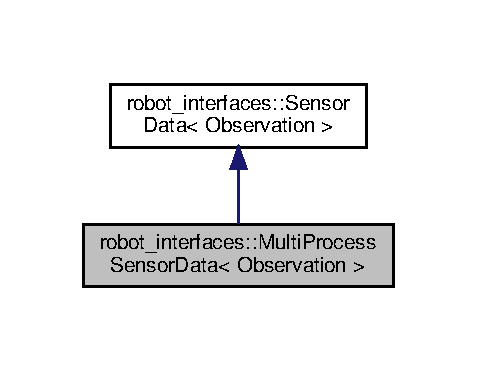
\includegraphics[width=229pt]{classrobot__interfaces_1_1MultiProcessSensorData__inherit__graph}
\end{center}
\end{figure}


Collaboration diagram for robot\+\_\+interfaces\+:\+:Multi\+Process\+Sensor\+Data$<$ Observation $>$\+:
\nopagebreak
\begin{figure}[H]
\begin{center}
\leavevmode
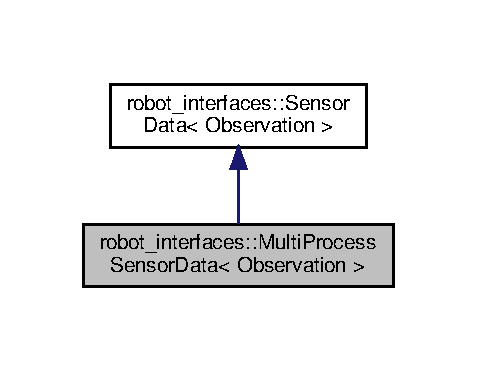
\includegraphics[width=229pt]{classrobot__interfaces_1_1MultiProcessSensorData__coll__graph}
\end{center}
\end{figure}
\subsection*{Public Member Functions}
\begin{DoxyCompactItemize}
\item 
\mbox{\Hypertarget{classrobot__interfaces_1_1MultiProcessSensorData_a8267ab3dc86230372571af2af73e07c0}\label{classrobot__interfaces_1_1MultiProcessSensorData_a8267ab3dc86230372571af2af73e07c0}} 
{\bfseries Multi\+Process\+Sensor\+Data} (const std\+::string \&shared\+\_\+memory\+\_\+id, bool is\+\_\+master, size\+\_\+t history\+\_\+length=1000)
\end{DoxyCompactItemize}
\subsection*{Additional Inherited Members}


\subsection{Detailed Description}
\subsubsection*{template$<$typename Observation$>$\newline
class robot\+\_\+interfaces\+::\+Multi\+Process\+Sensor\+Data$<$ Observation $>$}

\hyperlink{classrobot__interfaces_1_1SensorData}{Sensor\+Data} instance using multi process time series. 

Use this class if modules accessing the data are running in separate processes. When all modules run as threads in the same process, this class can be used as well, however, \hyperlink{classrobot__interfaces_1_1SingleProcessSensorData}{Single\+Process\+Sensor\+Data} might be more efficient in that case.

Contains the data coming from the sensors. 
\begin{DoxyTemplParams}{Template Parameters}
{\em Observation} & Type of the sensor observation. \\
\hline
\end{DoxyTemplParams}
\begin{DoxySeeAlso}{See also}
\hyperlink{classrobot__interfaces_1_1SingleProcessSensorData}{Single\+Process\+Sensor\+Data} 
\end{DoxySeeAlso}


The documentation for this class was generated from the following file\+:\begin{DoxyCompactItemize}
\item 
include/robot\+\_\+interfaces/sensors/\hyperlink{sensor__data_8hpp}{sensor\+\_\+data.\+hpp}\end{DoxyCompactItemize}

\hypertarget{structrobot__interfaces_1_1NFingerObservation}{}\section{robot\+\_\+interfaces\+:\+:N\+Finger\+Observation$<$ N\+\_\+\+F\+I\+N\+G\+E\+RS $>$ Struct Template Reference}
\label{structrobot__interfaces_1_1NFingerObservation}\index{robot\+\_\+interfaces\+::\+N\+Finger\+Observation$<$ N\+\_\+\+F\+I\+N\+G\+E\+R\+S $>$@{robot\+\_\+interfaces\+::\+N\+Finger\+Observation$<$ N\+\_\+\+F\+I\+N\+G\+E\+R\+S $>$}}


Observation of a Finger robot.  




{\ttfamily \#include $<$n\+\_\+finger\+\_\+observation.\+hpp$>$}



Inheritance diagram for robot\+\_\+interfaces\+:\+:N\+Finger\+Observation$<$ N\+\_\+\+F\+I\+N\+G\+E\+RS $>$\+:
\nopagebreak
\begin{figure}[H]
\begin{center}
\leavevmode
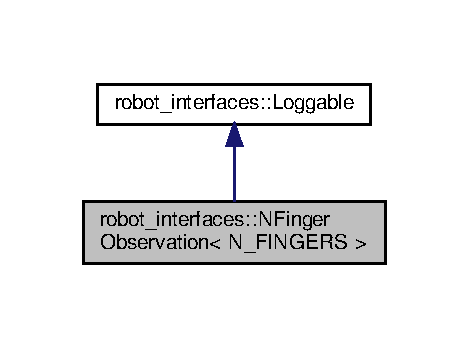
\includegraphics[width=225pt]{structrobot__interfaces_1_1NFingerObservation__inherit__graph}
\end{center}
\end{figure}


Collaboration diagram for robot\+\_\+interfaces\+:\+:N\+Finger\+Observation$<$ N\+\_\+\+F\+I\+N\+G\+E\+RS $>$\+:
\nopagebreak
\begin{figure}[H]
\begin{center}
\leavevmode
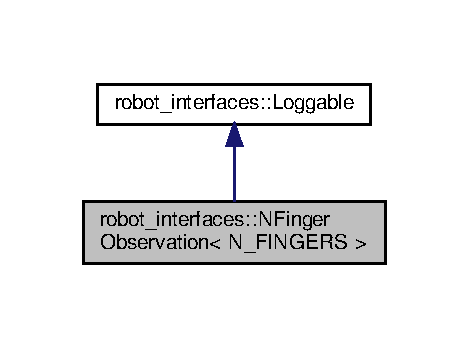
\includegraphics[width=225pt]{structrobot__interfaces_1_1NFingerObservation__coll__graph}
\end{center}
\end{figure}
\subsection*{Public Types}
\begin{DoxyCompactItemize}
\item 
\mbox{\Hypertarget{structrobot__interfaces_1_1NFingerObservation_a59675be5ce3ffe4c61fb1e88d131d31a}\label{structrobot__interfaces_1_1NFingerObservation_a59675be5ce3ffe4c61fb1e88d131d31a}} 
typedef Eigen\+::\+Matrix$<$ double, num\+\_\+joints, 1 $>$ {\bfseries Joint\+Vector}
\item 
\mbox{\Hypertarget{structrobot__interfaces_1_1NFingerObservation_aa97c4d41b53b370f0e7301a051f0e60a}\label{structrobot__interfaces_1_1NFingerObservation_aa97c4d41b53b370f0e7301a051f0e60a}} 
typedef Eigen\+::\+Matrix$<$ double, num\+\_\+fingers, 1 $>$ {\bfseries Finger\+Vector}
\end{DoxyCompactItemize}
\subsection*{Public Member Functions}
\begin{DoxyCompactItemize}
\item 
\mbox{\Hypertarget{structrobot__interfaces_1_1NFingerObservation_a66ebefed2f36a1c538cf4c0524931e60}\label{structrobot__interfaces_1_1NFingerObservation_a66ebefed2f36a1c538cf4c0524931e60}} 
{\footnotesize template$<$class Archive $>$ }\\void {\bfseries serialize} (Archive \&archive)
\item 
\mbox{\Hypertarget{structrobot__interfaces_1_1NFingerObservation_a0fd596a36ab38bdb148b64497499f32b}\label{structrobot__interfaces_1_1NFingerObservation_a0fd596a36ab38bdb148b64497499f32b}} 
std\+::vector$<$ std\+::string $>$ {\bfseries get\+\_\+name} () override
\item 
\mbox{\Hypertarget{structrobot__interfaces_1_1NFingerObservation_af8b4692b935585942a51b9342605b712}\label{structrobot__interfaces_1_1NFingerObservation_af8b4692b935585942a51b9342605b712}} 
std\+::vector$<$ std\+::vector$<$ double $>$ $>$ {\bfseries get\+\_\+data} () override
\end{DoxyCompactItemize}
\subsection*{Public Attributes}
\begin{DoxyCompactItemize}
\item 
\mbox{\Hypertarget{structrobot__interfaces_1_1NFingerObservation_ac830302468e0dee99c3c1e7e388267c3}\label{structrobot__interfaces_1_1NFingerObservation_ac830302468e0dee99c3c1e7e388267c3}} 
Joint\+Vector \hyperlink{structrobot__interfaces_1_1NFingerObservation_ac830302468e0dee99c3c1e7e388267c3}{position} = Joint\+Vector\+::\+Zero()
\begin{DoxyCompactList}\small\item\em Measured angular position of all joints in radian. \end{DoxyCompactList}\item 
\mbox{\Hypertarget{structrobot__interfaces_1_1NFingerObservation_a27ebb82cb119786e1ae9f85f89dfa76a}\label{structrobot__interfaces_1_1NFingerObservation_a27ebb82cb119786e1ae9f85f89dfa76a}} 
Joint\+Vector \hyperlink{structrobot__interfaces_1_1NFingerObservation_a27ebb82cb119786e1ae9f85f89dfa76a}{velocity} = Joint\+Vector\+::\+Zero()
\begin{DoxyCompactList}\small\item\em Measured velocity of all joints in radian/second. \end{DoxyCompactList}\item 
\mbox{\Hypertarget{structrobot__interfaces_1_1NFingerObservation_a693ccc700f9506bcc73cb12b63275194}\label{structrobot__interfaces_1_1NFingerObservation_a693ccc700f9506bcc73cb12b63275194}} 
Joint\+Vector \hyperlink{structrobot__interfaces_1_1NFingerObservation_a693ccc700f9506bcc73cb12b63275194}{torque} = Joint\+Vector\+::\+Zero()
\begin{DoxyCompactList}\small\item\em Measured torques of all joints in Nm. \end{DoxyCompactList}\item 
Finger\+Vector \hyperlink{structrobot__interfaces_1_1NFingerObservation_a48ea78dfbc3e17a313a312d758d27343}{tip\+\_\+force} = Finger\+Vector\+::\+Zero()
\begin{DoxyCompactList}\small\item\em Measurements of the pressure sensors at the finger tips. \end{DoxyCompactList}\end{DoxyCompactItemize}
\subsection*{Static Public Attributes}
\begin{DoxyCompactItemize}
\item 
\mbox{\Hypertarget{structrobot__interfaces_1_1NFingerObservation_ac3e7fa7d87b5af61378985e541152d46}\label{structrobot__interfaces_1_1NFingerObservation_ac3e7fa7d87b5af61378985e541152d46}} 
static constexpr size\+\_\+t {\bfseries num\+\_\+fingers} = N\+\_\+\+F\+I\+N\+G\+E\+RS
\item 
\mbox{\Hypertarget{structrobot__interfaces_1_1NFingerObservation_a52ba830179e60bdf07c90df1614bad11}\label{structrobot__interfaces_1_1NFingerObservation_a52ba830179e60bdf07c90df1614bad11}} 
static constexpr size\+\_\+t {\bfseries num\+\_\+joints} = N\+\_\+\+F\+I\+N\+G\+E\+RS $\ast$ 3
\end{DoxyCompactItemize}


\subsection{Detailed Description}
\subsubsection*{template$<$size\+\_\+t N\+\_\+\+F\+I\+N\+G\+E\+RS$>$\newline
struct robot\+\_\+interfaces\+::\+N\+Finger\+Observation$<$ N\+\_\+\+F\+I\+N\+G\+E\+R\+S $>$}

Observation of a Finger robot. 

Values like angular position, velocity or torque of the joints are represented as a 1-\/dimensional vector with one element per joint. The order of the joints in these vectors is as follows\+: \begin{DoxyVerb}0. Finger 1, upper joint
1. Finger 1, middle joint
2. Finger 1, lower joint
3. Finger 2, upper joint
4. Finger 2, middle joint
5. Finger 2, lower joint
...
#. Finger n, upper joint
#. Finger n, middle joint
#. Finger n, lower joint
\end{DoxyVerb}



\begin{DoxyTemplParams}{Template Parameters}
{\em N\+\_\+\+F\+I\+N\+G\+E\+RS} & Number of fingers. \\
\hline
\end{DoxyTemplParams}


\subsection{Member Data Documentation}
\mbox{\Hypertarget{structrobot__interfaces_1_1NFingerObservation_a48ea78dfbc3e17a313a312d758d27343}\label{structrobot__interfaces_1_1NFingerObservation_a48ea78dfbc3e17a313a312d758d27343}} 
\index{robot\+\_\+interfaces\+::\+N\+Finger\+Observation@{robot\+\_\+interfaces\+::\+N\+Finger\+Observation}!tip\+\_\+force@{tip\+\_\+force}}
\index{tip\+\_\+force@{tip\+\_\+force}!robot\+\_\+interfaces\+::\+N\+Finger\+Observation@{robot\+\_\+interfaces\+::\+N\+Finger\+Observation}}
\subsubsection{\texorpdfstring{tip\+\_\+force}{tip\_force}}
{\footnotesize\ttfamily template$<$size\+\_\+t N\+\_\+\+F\+I\+N\+G\+E\+RS$>$ \\
Finger\+Vector \hyperlink{structrobot__interfaces_1_1NFingerObservation}{robot\+\_\+interfaces\+::\+N\+Finger\+Observation}$<$ N\+\_\+\+F\+I\+N\+G\+E\+RS $>$\+::tip\+\_\+force = Finger\+Vector\+::\+Zero()}



Measurements of the pressure sensors at the finger tips. 

One per finger. Ranges between 0 and 1 without specific unit. Note that not all fingers are equipped with an actual sensor! For fingers without sensor, this value is undefined. 

The documentation for this struct was generated from the following file\+:\begin{DoxyCompactItemize}
\item 
include/robot\+\_\+interfaces/\hyperlink{n__finger__observation_8hpp}{n\+\_\+finger\+\_\+observation.\+hpp}\end{DoxyCompactItemize}

\hypertarget{structrobot__interfaces_1_1NJointAction}{}\section{robot\+\_\+interfaces\+:\+:N\+Joint\+Action$<$ N $>$ Struct Template Reference}
\label{structrobot__interfaces_1_1NJointAction}\index{robot\+\_\+interfaces\+::\+N\+Joint\+Action$<$ N $>$@{robot\+\_\+interfaces\+::\+N\+Joint\+Action$<$ N $>$}}


Action of a generic n-\/joint robot.  




{\ttfamily \#include $<$n\+\_\+joint\+\_\+action.\+hpp$>$}



Inheritance diagram for robot\+\_\+interfaces\+:\+:N\+Joint\+Action$<$ N $>$\+:
\nopagebreak
\begin{figure}[H]
\begin{center}
\leavevmode
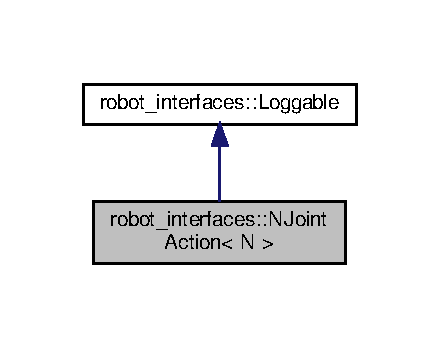
\includegraphics[width=211pt]{structrobot__interfaces_1_1NJointAction__inherit__graph}
\end{center}
\end{figure}


Collaboration diagram for robot\+\_\+interfaces\+:\+:N\+Joint\+Action$<$ N $>$\+:
\nopagebreak
\begin{figure}[H]
\begin{center}
\leavevmode
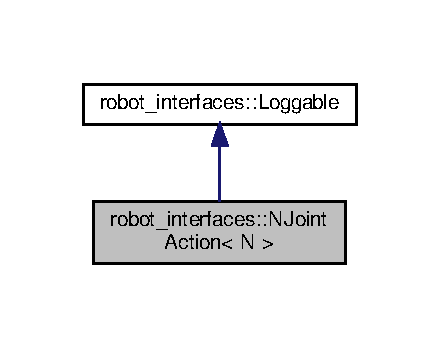
\includegraphics[width=211pt]{structrobot__interfaces_1_1NJointAction__coll__graph}
\end{center}
\end{figure}
\subsection*{Public Types}
\begin{DoxyCompactItemize}
\item 
\mbox{\Hypertarget{structrobot__interfaces_1_1NJointAction_afdfe44811a3d9063f2a12dc05be515cb}\label{structrobot__interfaces_1_1NJointAction_afdfe44811a3d9063f2a12dc05be515cb}} 
typedef Eigen\+::\+Matrix$<$ double, N, 1 $>$ {\bfseries Vector}
\end{DoxyCompactItemize}
\subsection*{Public Member Functions}
\begin{DoxyCompactItemize}
\item 
\mbox{\Hypertarget{structrobot__interfaces_1_1NJointAction_aca14e1c3aa3f7ac545405e8a5c9575a6}\label{structrobot__interfaces_1_1NJointAction_aca14e1c3aa3f7ac545405e8a5c9575a6}} 
{\footnotesize template$<$class Archive $>$ }\\void {\bfseries serialize} (Archive \&archive)
\item 
\mbox{\Hypertarget{structrobot__interfaces_1_1NJointAction_a8c19d0c69b6fac9a86e7a0017d275ac4}\label{structrobot__interfaces_1_1NJointAction_a8c19d0c69b6fac9a86e7a0017d275ac4}} 
std\+::vector$<$ std\+::string $>$ {\bfseries get\+\_\+name} () override
\item 
\mbox{\Hypertarget{structrobot__interfaces_1_1NJointAction_a309b4188b2a508aa85cbedb0f6ef6343}\label{structrobot__interfaces_1_1NJointAction_a309b4188b2a508aa85cbedb0f6ef6343}} 
std\+::vector$<$ std\+::vector$<$ double $>$ $>$ {\bfseries get\+\_\+data} () override
\item 
\hyperlink{structrobot__interfaces_1_1NJointAction_a518f1d5bd4161809c176a4007f58fb0d}{N\+Joint\+Action} (Vector \hyperlink{structrobot__interfaces_1_1NJointAction_aab60be78c0008092bf3f36b92a25245d}{torque}=Vector\+::\+Zero(), Vector \hyperlink{structrobot__interfaces_1_1NJointAction_a1ba640ac58fef08cd8a5c964b7a4096f}{position}=\hyperlink{structrobot__interfaces_1_1NJointAction_abb5403bb946dc4b9e9e5e13b9195ad86}{None}(), Vector \hyperlink{structrobot__interfaces_1_1NJointAction_a4100b04d42c8e1d9b04ba141212c3461}{position\+\_\+kp}=\hyperlink{structrobot__interfaces_1_1NJointAction_abb5403bb946dc4b9e9e5e13b9195ad86}{None}(), Vector \hyperlink{structrobot__interfaces_1_1NJointAction_a652131480e656840e53f8709dae9c487}{position\+\_\+kd}=\hyperlink{structrobot__interfaces_1_1NJointAction_abb5403bb946dc4b9e9e5e13b9195ad86}{None}())
\begin{DoxyCompactList}\small\item\em Create action with desired torque and (optional) position. \end{DoxyCompactList}\end{DoxyCompactItemize}
\subsection*{Static Public Member Functions}
\begin{DoxyCompactItemize}
\item 
static \hyperlink{structrobot__interfaces_1_1NJointAction}{N\+Joint\+Action} \hyperlink{structrobot__interfaces_1_1NJointAction_ad1e48599cf7ce7b154464db23978a3c2}{Torque} (Vector \hyperlink{structrobot__interfaces_1_1NJointAction_aab60be78c0008092bf3f36b92a25245d}{torque})
\begin{DoxyCompactList}\small\item\em Create an action that only contains a torque command. \end{DoxyCompactList}\item 
static \hyperlink{structrobot__interfaces_1_1NJointAction}{N\+Joint\+Action} \hyperlink{structrobot__interfaces_1_1NJointAction_ab90dfaabbae281108bf83337f455143c}{Position} (Vector \hyperlink{structrobot__interfaces_1_1NJointAction_a1ba640ac58fef08cd8a5c964b7a4096f}{position}, Vector kp=\hyperlink{structrobot__interfaces_1_1NJointAction_abb5403bb946dc4b9e9e5e13b9195ad86}{None}(), Vector kd=\hyperlink{structrobot__interfaces_1_1NJointAction_abb5403bb946dc4b9e9e5e13b9195ad86}{None}())
\begin{DoxyCompactList}\small\item\em Create an action that only contains a position command. \end{DoxyCompactList}\item 
static \hyperlink{structrobot__interfaces_1_1NJointAction}{N\+Joint\+Action} \hyperlink{structrobot__interfaces_1_1NJointAction_a4c779f6bc160922b65d3a78d0b561f01}{Torque\+And\+Position} (Vector \hyperlink{structrobot__interfaces_1_1NJointAction_aab60be78c0008092bf3f36b92a25245d}{torque}, Vector \hyperlink{structrobot__interfaces_1_1NJointAction_a1ba640ac58fef08cd8a5c964b7a4096f}{position}, Vector \hyperlink{structrobot__interfaces_1_1NJointAction_a4100b04d42c8e1d9b04ba141212c3461}{position\+\_\+kp}=\hyperlink{structrobot__interfaces_1_1NJointAction_abb5403bb946dc4b9e9e5e13b9195ad86}{None}(), Vector \hyperlink{structrobot__interfaces_1_1NJointAction_a652131480e656840e53f8709dae9c487}{position\+\_\+kd}=\hyperlink{structrobot__interfaces_1_1NJointAction_abb5403bb946dc4b9e9e5e13b9195ad86}{None}())
\begin{DoxyCompactList}\small\item\em Create an action with both torque and position commands. \end{DoxyCompactList}\item 
static \hyperlink{structrobot__interfaces_1_1NJointAction}{N\+Joint\+Action} \hyperlink{structrobot__interfaces_1_1NJointAction_a7def88d6d46acd3e77db3dc49d04dd88}{Zero} ()
\begin{DoxyCompactList}\small\item\em Create a zero-\/torque action. \end{DoxyCompactList}\item 
static Vector \hyperlink{structrobot__interfaces_1_1NJointAction_abb5403bb946dc4b9e9e5e13b9195ad86}{None} ()
\begin{DoxyCompactList}\small\item\em Create a Na\+N-\/\+Vector. \end{DoxyCompactList}\end{DoxyCompactItemize}
\subsection*{Public Attributes}
\begin{DoxyCompactItemize}
\item 
\mbox{\Hypertarget{structrobot__interfaces_1_1NJointAction_aab60be78c0008092bf3f36b92a25245d}\label{structrobot__interfaces_1_1NJointAction_aab60be78c0008092bf3f36b92a25245d}} 
Vector \hyperlink{structrobot__interfaces_1_1NJointAction_aab60be78c0008092bf3f36b92a25245d}{torque}
\begin{DoxyCompactList}\small\item\em Desired torque command (in addition to position controller). \end{DoxyCompactList}\item 
\mbox{\Hypertarget{structrobot__interfaces_1_1NJointAction_a1ba640ac58fef08cd8a5c964b7a4096f}\label{structrobot__interfaces_1_1NJointAction_a1ba640ac58fef08cd8a5c964b7a4096f}} 
Vector \hyperlink{structrobot__interfaces_1_1NJointAction_a1ba640ac58fef08cd8a5c964b7a4096f}{position}
\begin{DoxyCompactList}\small\item\em Desired position. Set to NaN to disable position controller. \end{DoxyCompactList}\item 
\mbox{\Hypertarget{structrobot__interfaces_1_1NJointAction_a4100b04d42c8e1d9b04ba141212c3461}\label{structrobot__interfaces_1_1NJointAction_a4100b04d42c8e1d9b04ba141212c3461}} 
Vector \hyperlink{structrobot__interfaces_1_1NJointAction_a4100b04d42c8e1d9b04ba141212c3461}{position\+\_\+kp}
\begin{DoxyCompactList}\small\item\em P-\/gain for position controller. If NaN, default is used. \end{DoxyCompactList}\item 
\mbox{\Hypertarget{structrobot__interfaces_1_1NJointAction_a652131480e656840e53f8709dae9c487}\label{structrobot__interfaces_1_1NJointAction_a652131480e656840e53f8709dae9c487}} 
Vector \hyperlink{structrobot__interfaces_1_1NJointAction_a652131480e656840e53f8709dae9c487}{position\+\_\+kd}
\begin{DoxyCompactList}\small\item\em D-\/gain for position controller. If NaN, default is used. \end{DoxyCompactList}\end{DoxyCompactItemize}
\subsection*{Static Public Attributes}
\begin{DoxyCompactItemize}
\item 
\mbox{\Hypertarget{structrobot__interfaces_1_1NJointAction_a8d5a5328cfc71d1b892b2581e9b22723}\label{structrobot__interfaces_1_1NJointAction_a8d5a5328cfc71d1b892b2581e9b22723}} 
static constexpr size\+\_\+t \hyperlink{structrobot__interfaces_1_1NJointAction_a8d5a5328cfc71d1b892b2581e9b22723}{num\+\_\+joints} = N
\begin{DoxyCompactList}\small\item\em Number of joints. \end{DoxyCompactList}\end{DoxyCompactItemize}


\subsection{Detailed Description}
\subsubsection*{template$<$size\+\_\+t N$>$\newline
struct robot\+\_\+interfaces\+::\+N\+Joint\+Action$<$ N $>$}

Action of a generic n-\/joint robot. 

This action type can be used for all n-\/joint robots that expect torque or position commands on joint-\/level.


\begin{DoxyTemplParams}{Template Parameters}
{\em N} & Number of joints. \\
\hline
\end{DoxyTemplParams}


\subsection{Constructor \& Destructor Documentation}
\mbox{\Hypertarget{structrobot__interfaces_1_1NJointAction_a518f1d5bd4161809c176a4007f58fb0d}\label{structrobot__interfaces_1_1NJointAction_a518f1d5bd4161809c176a4007f58fb0d}} 
\index{robot\+\_\+interfaces\+::\+N\+Joint\+Action@{robot\+\_\+interfaces\+::\+N\+Joint\+Action}!N\+Joint\+Action@{N\+Joint\+Action}}
\index{N\+Joint\+Action@{N\+Joint\+Action}!robot\+\_\+interfaces\+::\+N\+Joint\+Action@{robot\+\_\+interfaces\+::\+N\+Joint\+Action}}
\subsubsection{\texorpdfstring{N\+Joint\+Action()}{NJointAction()}}
{\footnotesize\ttfamily template$<$size\+\_\+t N$>$ \\
\hyperlink{structrobot__interfaces_1_1NJointAction}{robot\+\_\+interfaces\+::\+N\+Joint\+Action}$<$ N $>$\+::\hyperlink{structrobot__interfaces_1_1NJointAction}{N\+Joint\+Action} (\begin{DoxyParamCaption}\item[{Vector}]{torque = {\ttfamily Vector\+:\+:Zero()},  }\item[{Vector}]{position = {\ttfamily \hyperlink{structrobot__interfaces_1_1NJointAction_abb5403bb946dc4b9e9e5e13b9195ad86}{None}()},  }\item[{Vector}]{position\+\_\+kp = {\ttfamily \hyperlink{structrobot__interfaces_1_1NJointAction_abb5403bb946dc4b9e9e5e13b9195ad86}{None}()},  }\item[{Vector}]{position\+\_\+kd = {\ttfamily \hyperlink{structrobot__interfaces_1_1NJointAction_abb5403bb946dc4b9e9e5e13b9195ad86}{None}()} }\end{DoxyParamCaption})\hspace{0.3cm}{\ttfamily [inline]}}



Create action with desired torque and (optional) position. 

The resulting torque command sent to the robot is \begin{DoxyVerb}sent_torque = torque + PD(position)
\end{DoxyVerb}


To disable the position controller, set the target position to NaN. The controller is executed joint-\/wise, so it is possible to run it only for some joints by setting a target position for these joints and setting the others to NaN.

The specified torque is always added to the result of the position controller, so if you only want to run the position controller, make sure to set {\ttfamily torque} to zero for all joints.

For more explicit code, the static factory methods {\ttfamily Troque}, {\ttfamily Position}, {\ttfamily Torque\+And\+Position} and {\ttfamily Zero} should be used instead directly creating actions through this constuctor.


\begin{DoxyParams}{Parameters}
{\em torque} & Desired torque. \\
\hline
{\em position} & Desired position. Set values to NaN to disable position controller for the corresponding joints \\
\hline
{\em position\+\_\+kp} & P-\/gains for the position controller. Set to NaN to use default values. \\
\hline
{\em position\+\_\+kd} & D-\/gains for the position controller. Set to NaN to use default values. \\
\hline
\end{DoxyParams}


\subsection{Member Function Documentation}
\mbox{\Hypertarget{structrobot__interfaces_1_1NJointAction_abb5403bb946dc4b9e9e5e13b9195ad86}\label{structrobot__interfaces_1_1NJointAction_abb5403bb946dc4b9e9e5e13b9195ad86}} 
\index{robot\+\_\+interfaces\+::\+N\+Joint\+Action@{robot\+\_\+interfaces\+::\+N\+Joint\+Action}!None@{None}}
\index{None@{None}!robot\+\_\+interfaces\+::\+N\+Joint\+Action@{robot\+\_\+interfaces\+::\+N\+Joint\+Action}}
\subsubsection{\texorpdfstring{None()}{None()}}
{\footnotesize\ttfamily template$<$size\+\_\+t N$>$ \\
static Vector \hyperlink{structrobot__interfaces_1_1NJointAction}{robot\+\_\+interfaces\+::\+N\+Joint\+Action}$<$ N $>$\+::None (\begin{DoxyParamCaption}{ }\end{DoxyParamCaption})\hspace{0.3cm}{\ttfamily [inline]}, {\ttfamily [static]}}



Create a Na\+N-\/\+Vector. 

Helper function to set defaults for position.

\begin{DoxyReturn}{Returns}
Vector with all elements set to NaN. 
\end{DoxyReturn}
\mbox{\Hypertarget{structrobot__interfaces_1_1NJointAction_ab90dfaabbae281108bf83337f455143c}\label{structrobot__interfaces_1_1NJointAction_ab90dfaabbae281108bf83337f455143c}} 
\index{robot\+\_\+interfaces\+::\+N\+Joint\+Action@{robot\+\_\+interfaces\+::\+N\+Joint\+Action}!Position@{Position}}
\index{Position@{Position}!robot\+\_\+interfaces\+::\+N\+Joint\+Action@{robot\+\_\+interfaces\+::\+N\+Joint\+Action}}
\subsubsection{\texorpdfstring{Position()}{Position()}}
{\footnotesize\ttfamily template$<$size\+\_\+t N$>$ \\
static \hyperlink{structrobot__interfaces_1_1NJointAction}{N\+Joint\+Action} \hyperlink{structrobot__interfaces_1_1NJointAction}{robot\+\_\+interfaces\+::\+N\+Joint\+Action}$<$ N $>$\+::Position (\begin{DoxyParamCaption}\item[{Vector}]{position,  }\item[{Vector}]{kp = {\ttfamily \hyperlink{structrobot__interfaces_1_1NJointAction_abb5403bb946dc4b9e9e5e13b9195ad86}{None}()},  }\item[{Vector}]{kd = {\ttfamily \hyperlink{structrobot__interfaces_1_1NJointAction_abb5403bb946dc4b9e9e5e13b9195ad86}{None}()} }\end{DoxyParamCaption})\hspace{0.3cm}{\ttfamily [inline]}, {\ttfamily [static]}}



Create an action that only contains a position command. 


\begin{DoxyParams}{Parameters}
{\em position} & Desired position. \\
\hline
{\em kp} & P-\/gain for position controller. If not set, default is used. Set to NaN for specific joints to use default for this joint. \\
\hline
{\em kd} & D-\/gain for position controller. If not set, default is used. Set to NaN for specific joints to use default for this joint.\\
\hline
\end{DoxyParams}
\begin{DoxyReturn}{Returns}
Pure \char`\"{}position action\char`\"{}. 
\end{DoxyReturn}
\mbox{\Hypertarget{structrobot__interfaces_1_1NJointAction_ad1e48599cf7ce7b154464db23978a3c2}\label{structrobot__interfaces_1_1NJointAction_ad1e48599cf7ce7b154464db23978a3c2}} 
\index{robot\+\_\+interfaces\+::\+N\+Joint\+Action@{robot\+\_\+interfaces\+::\+N\+Joint\+Action}!Torque@{Torque}}
\index{Torque@{Torque}!robot\+\_\+interfaces\+::\+N\+Joint\+Action@{robot\+\_\+interfaces\+::\+N\+Joint\+Action}}
\subsubsection{\texorpdfstring{Torque()}{Torque()}}
{\footnotesize\ttfamily template$<$size\+\_\+t N$>$ \\
static \hyperlink{structrobot__interfaces_1_1NJointAction}{N\+Joint\+Action} \hyperlink{structrobot__interfaces_1_1NJointAction}{robot\+\_\+interfaces\+::\+N\+Joint\+Action}$<$ N $>$\+::Torque (\begin{DoxyParamCaption}\item[{Vector}]{torque }\end{DoxyParamCaption})\hspace{0.3cm}{\ttfamily [inline]}, {\ttfamily [static]}}



Create an action that only contains a torque command. 


\begin{DoxyParams}{Parameters}
{\em torque} & Desired torque.\\
\hline
\end{DoxyParams}
\begin{DoxyReturn}{Returns}
Pure \char`\"{}torque action\char`\"{}. 
\end{DoxyReturn}
\mbox{\Hypertarget{structrobot__interfaces_1_1NJointAction_a4c779f6bc160922b65d3a78d0b561f01}\label{structrobot__interfaces_1_1NJointAction_a4c779f6bc160922b65d3a78d0b561f01}} 
\index{robot\+\_\+interfaces\+::\+N\+Joint\+Action@{robot\+\_\+interfaces\+::\+N\+Joint\+Action}!Torque\+And\+Position@{Torque\+And\+Position}}
\index{Torque\+And\+Position@{Torque\+And\+Position}!robot\+\_\+interfaces\+::\+N\+Joint\+Action@{robot\+\_\+interfaces\+::\+N\+Joint\+Action}}
\subsubsection{\texorpdfstring{Torque\+And\+Position()}{TorqueAndPosition()}}
{\footnotesize\ttfamily template$<$size\+\_\+t N$>$ \\
static \hyperlink{structrobot__interfaces_1_1NJointAction}{N\+Joint\+Action} \hyperlink{structrobot__interfaces_1_1NJointAction}{robot\+\_\+interfaces\+::\+N\+Joint\+Action}$<$ N $>$\+::Torque\+And\+Position (\begin{DoxyParamCaption}\item[{Vector}]{torque,  }\item[{Vector}]{position,  }\item[{Vector}]{position\+\_\+kp = {\ttfamily \hyperlink{structrobot__interfaces_1_1NJointAction_abb5403bb946dc4b9e9e5e13b9195ad86}{None}()},  }\item[{Vector}]{position\+\_\+kd = {\ttfamily \hyperlink{structrobot__interfaces_1_1NJointAction_abb5403bb946dc4b9e9e5e13b9195ad86}{None}()} }\end{DoxyParamCaption})\hspace{0.3cm}{\ttfamily [inline]}, {\ttfamily [static]}}



Create an action with both torque and position commands. 


\begin{DoxyParams}{Parameters}
{\em torque} & Desired torque. \\
\hline
{\em position} & Desired position. Set to NaN for specific joints to disable position control for this joint. \\
\hline
{\em kp} & P-\/gain for position controller. If not set, default is used. Set to NaN for specific joints to use default for this joint. \\
\hline
{\em kd} & D-\/gain for position controller. If not set, default is used. Set to NaN for specific joints to use default for this joint.\\
\hline
\end{DoxyParams}
\begin{DoxyReturn}{Returns}
Action with both torque and position commands. 
\end{DoxyReturn}
\mbox{\Hypertarget{structrobot__interfaces_1_1NJointAction_a7def88d6d46acd3e77db3dc49d04dd88}\label{structrobot__interfaces_1_1NJointAction_a7def88d6d46acd3e77db3dc49d04dd88}} 
\index{robot\+\_\+interfaces\+::\+N\+Joint\+Action@{robot\+\_\+interfaces\+::\+N\+Joint\+Action}!Zero@{Zero}}
\index{Zero@{Zero}!robot\+\_\+interfaces\+::\+N\+Joint\+Action@{robot\+\_\+interfaces\+::\+N\+Joint\+Action}}
\subsubsection{\texorpdfstring{Zero()}{Zero()}}
{\footnotesize\ttfamily template$<$size\+\_\+t N$>$ \\
static \hyperlink{structrobot__interfaces_1_1NJointAction}{N\+Joint\+Action} \hyperlink{structrobot__interfaces_1_1NJointAction}{robot\+\_\+interfaces\+::\+N\+Joint\+Action}$<$ N $>$\+::Zero (\begin{DoxyParamCaption}{ }\end{DoxyParamCaption})\hspace{0.3cm}{\ttfamily [inline]}, {\ttfamily [static]}}



Create a zero-\/torque action. 

\begin{DoxyReturn}{Returns}
Zero-\/torque action with position control disabled. 
\end{DoxyReturn}


The documentation for this struct was generated from the following file\+:\begin{DoxyCompactItemize}
\item 
include/robot\+\_\+interfaces/\hyperlink{n__joint__action_8hpp}{n\+\_\+joint\+\_\+action.\+hpp}\end{DoxyCompactItemize}

\hypertarget{structrobot__interfaces_1_1NJointObservation}{}\section{robot\+\_\+interfaces\+:\+:N\+Joint\+Observation$<$ N $>$ Struct Template Reference}
\label{structrobot__interfaces_1_1NJointObservation}\index{robot\+\_\+interfaces\+::\+N\+Joint\+Observation$<$ N $>$@{robot\+\_\+interfaces\+::\+N\+Joint\+Observation$<$ N $>$}}


Basic observation for a generic n-\/joint robot.  




{\ttfamily \#include $<$n\+\_\+joint\+\_\+observation.\+hpp$>$}



Inheritance diagram for robot\+\_\+interfaces\+:\+:N\+Joint\+Observation$<$ N $>$\+:
\nopagebreak
\begin{figure}[H]
\begin{center}
\leavevmode
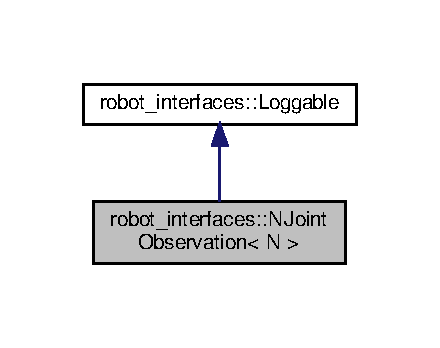
\includegraphics[width=211pt]{structrobot__interfaces_1_1NJointObservation__inherit__graph}
\end{center}
\end{figure}


Collaboration diagram for robot\+\_\+interfaces\+:\+:N\+Joint\+Observation$<$ N $>$\+:
\nopagebreak
\begin{figure}[H]
\begin{center}
\leavevmode
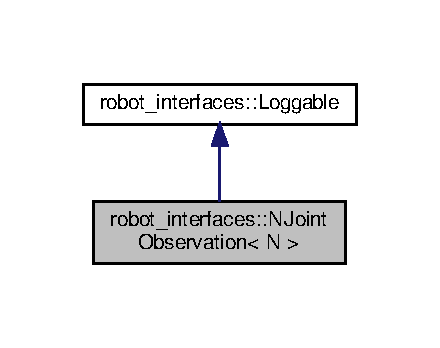
\includegraphics[width=211pt]{structrobot__interfaces_1_1NJointObservation__coll__graph}
\end{center}
\end{figure}
\subsection*{Public Types}
\begin{DoxyCompactItemize}
\item 
\mbox{\Hypertarget{structrobot__interfaces_1_1NJointObservation_aa17734049f437f1f2a7fee0009ff91fe}\label{structrobot__interfaces_1_1NJointObservation_aa17734049f437f1f2a7fee0009ff91fe}} 
typedef Eigen\+::\+Matrix$<$ double, N, 1 $>$ {\bfseries Vector}
\end{DoxyCompactItemize}
\subsection*{Public Member Functions}
\begin{DoxyCompactItemize}
\item 
\mbox{\Hypertarget{structrobot__interfaces_1_1NJointObservation_a0c3b4adc3922ac32f11ba5de22d60625}\label{structrobot__interfaces_1_1NJointObservation_a0c3b4adc3922ac32f11ba5de22d60625}} 
{\footnotesize template$<$class Archive $>$ }\\void {\bfseries serialize} (Archive \&archive)
\item 
\mbox{\Hypertarget{structrobot__interfaces_1_1NJointObservation_a610b88db60db090f64a03d4a286332be}\label{structrobot__interfaces_1_1NJointObservation_a610b88db60db090f64a03d4a286332be}} 
std\+::vector$<$ std\+::string $>$ {\bfseries get\+\_\+name} () override
\item 
\mbox{\Hypertarget{structrobot__interfaces_1_1NJointObservation_a5294b6b4e403b79f199dff888984bbf1}\label{structrobot__interfaces_1_1NJointObservation_a5294b6b4e403b79f199dff888984bbf1}} 
std\+::vector$<$ std\+::vector$<$ double $>$ $>$ {\bfseries get\+\_\+data} () override
\end{DoxyCompactItemize}
\subsection*{Public Attributes}
\begin{DoxyCompactItemize}
\item 
\mbox{\Hypertarget{structrobot__interfaces_1_1NJointObservation_ab7b9151ce91a3b545364cab6163ba86f}\label{structrobot__interfaces_1_1NJointObservation_ab7b9151ce91a3b545364cab6163ba86f}} 
Vector {\bfseries position} = Vector\+::\+Zero()
\item 
\mbox{\Hypertarget{structrobot__interfaces_1_1NJointObservation_a96d7c53ef241b77432105dfa01b36cb0}\label{structrobot__interfaces_1_1NJointObservation_a96d7c53ef241b77432105dfa01b36cb0}} 
Vector {\bfseries velocity} = Vector\+::\+Zero()
\item 
\mbox{\Hypertarget{structrobot__interfaces_1_1NJointObservation_aaef74cc4c90e2dd4b4c6132773c7b262}\label{structrobot__interfaces_1_1NJointObservation_aaef74cc4c90e2dd4b4c6132773c7b262}} 
Vector {\bfseries torque} = Vector\+::\+Zero()
\end{DoxyCompactItemize}
\subsection*{Static Public Attributes}
\begin{DoxyCompactItemize}
\item 
\mbox{\Hypertarget{structrobot__interfaces_1_1NJointObservation_ab82f5a0d187661046f76cd5f92701b1c}\label{structrobot__interfaces_1_1NJointObservation_ab82f5a0d187661046f76cd5f92701b1c}} 
static constexpr size\+\_\+t \hyperlink{structrobot__interfaces_1_1NJointObservation_ab82f5a0d187661046f76cd5f92701b1c}{num\+\_\+joints} = N
\begin{DoxyCompactList}\small\item\em Number of joints. \end{DoxyCompactList}\end{DoxyCompactItemize}


\subsection{Detailed Description}
\subsubsection*{template$<$size\+\_\+t N$>$\newline
struct robot\+\_\+interfaces\+::\+N\+Joint\+Observation$<$ N $>$}

Basic observation for a generic n-\/joint robot. 

Simple observation type with position, velocity and torque for each joint.


\begin{DoxyTemplParams}{Template Parameters}
{\em N} & Number of joints. \\
\hline
\end{DoxyTemplParams}


The documentation for this struct was generated from the following file\+:\begin{DoxyCompactItemize}
\item 
include/robot\+\_\+interfaces/\hyperlink{n__joint__observation_8hpp}{n\+\_\+joint\+\_\+observation.\+hpp}\end{DoxyCompactItemize}

\hypertarget{classrobot__interfaces_1_1example_1_1Observation}{}\section{robot\+\_\+interfaces\+:\+:example\+:\+:Observation Class Reference}
\label{classrobot__interfaces_1_1example_1_1Observation}\index{robot\+\_\+interfaces\+::example\+::\+Observation@{robot\+\_\+interfaces\+::example\+::\+Observation}}


\hyperlink{classrobot__interfaces_1_1example_1_1Observation}{Observation} read from the robot by \hyperlink{classrobot__interfaces_1_1example_1_1Driver}{Driver}.  




{\ttfamily \#include $<$example.\+hpp$>$}

\subsection*{Public Member Functions}
\begin{DoxyCompactItemize}
\item 
\mbox{\Hypertarget{classrobot__interfaces_1_1example_1_1Observation_af363ed16350ab130e4a6ba4e2e6bbe0e}\label{classrobot__interfaces_1_1example_1_1Observation_af363ed16350ab130e4a6ba4e2e6bbe0e}} 
void {\bfseries print} (bool backline)
\end{DoxyCompactItemize}
\subsection*{Public Attributes}
\begin{DoxyCompactItemize}
\item 
\mbox{\Hypertarget{classrobot__interfaces_1_1example_1_1Observation_ae7dd8df574cd0a303999e945188c353e}\label{classrobot__interfaces_1_1example_1_1Observation_ae7dd8df574cd0a303999e945188c353e}} 
int {\bfseries values} \mbox{[}2\mbox{]}
\end{DoxyCompactItemize}


\subsection{Detailed Description}
\hyperlink{classrobot__interfaces_1_1example_1_1Observation}{Observation} read from the robot by \hyperlink{classrobot__interfaces_1_1example_1_1Driver}{Driver}. 

An observation is the current position for each D\+OF. \begin{Desc}
\item[Examples\+: ]\par
\hyperlink{demo_8cpp-example}{demo.\+cpp}.\end{Desc}


The documentation for this class was generated from the following file\+:\begin{DoxyCompactItemize}
\item 
include/robot\+\_\+interfaces/\hyperlink{example_8hpp}{example.\+hpp}\end{DoxyCompactItemize}

\hypertarget{classrobot__interfaces_1_1demo_1_1Observation}{}\section{robot\+\_\+interfaces\+:\+:demo\+:\+:Observation Class Reference}
\label{classrobot__interfaces_1_1demo_1_1Observation}\index{robot\+\_\+interfaces\+::demo\+::\+Observation@{robot\+\_\+interfaces\+::demo\+::\+Observation}}


Read from the robot by \hyperlink{classDriver}{Driver}.  




{\ttfamily \#include $<$types.\+hpp$>$}

\subsection*{Public Member Functions}
\begin{DoxyCompactItemize}
\item 
\mbox{\Hypertarget{classrobot__interfaces_1_1demo_1_1Observation_a1bec6db0664543ac4d47c222b66b5af4}\label{classrobot__interfaces_1_1demo_1_1Observation_a1bec6db0664543ac4d47c222b66b5af4}} 
void {\bfseries print} (bool backline) const
\item 
\mbox{\Hypertarget{classrobot__interfaces_1_1demo_1_1Observation_adc50512a62b26a896da47f6f67dee44e}\label{classrobot__interfaces_1_1demo_1_1Observation_adc50512a62b26a896da47f6f67dee44e}} 
{\footnotesize template$<$class Archive $>$ }\\void {\bfseries serialize} (Archive \&ar)
\end{DoxyCompactItemize}
\subsection*{Public Attributes}
\begin{DoxyCompactItemize}
\item 
\mbox{\Hypertarget{classrobot__interfaces_1_1demo_1_1Observation_a930664896eceed4f3ee0de6f0e29bea4}\label{classrobot__interfaces_1_1demo_1_1Observation_a930664896eceed4f3ee0de6f0e29bea4}} 
int {\bfseries values} \mbox{[}2\mbox{]}
\end{DoxyCompactItemize}


\subsection{Detailed Description}
Read from the robot by \hyperlink{classDriver}{Driver}. 

An observation is the current position for each dof. \begin{Desc}
\item[Examples\+: ]\par
\hyperlink{demo_multiprocess_backend_8cpp-example}{demo\+\_\+multiprocess\+\_\+backend.\+cpp}, and \hyperlink{demo_multiprocess_frontend_8cpp-example}{demo\+\_\+multiprocess\+\_\+frontend.\+cpp}.\end{Desc}


The documentation for this class was generated from the following file\+:\begin{DoxyCompactItemize}
\item 
demos/\hyperlink{demos_2types_8hpp}{types.\+hpp}\end{DoxyCompactItemize}

\hypertarget{classrobot__interfaces_1_1Robot}{}\section{robot\+\_\+interfaces\+:\+:Robot$<$ Action, Observation, Driver, Data $>$ Class Template Reference}
\label{classrobot__interfaces_1_1Robot}\index{robot\+\_\+interfaces\+::\+Robot$<$ Action, Observation, Driver, Data $>$@{robot\+\_\+interfaces\+::\+Robot$<$ Action, Observation, Driver, Data $>$}}


\hyperlink{classrobot__interfaces_1_1RobotFrontend}{Robot\+Frontend} that construct and encapsulates its related \hyperlink{classrobot__interfaces_1_1RobotBackend}{Robot\+Backend}.  




{\ttfamily \#include $<$robot.\+hpp$>$}



Inheritance diagram for robot\+\_\+interfaces\+:\+:Robot$<$ Action, Observation, Driver, Data $>$\+:
\nopagebreak
\begin{figure}[H]
\begin{center}
\leavevmode
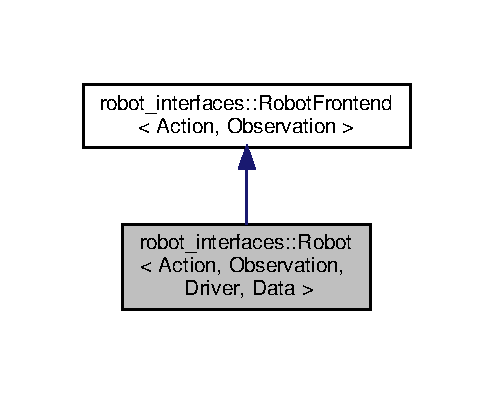
\includegraphics[width=237pt]{classrobot__interfaces_1_1Robot__inherit__graph}
\end{center}
\end{figure}


Collaboration diagram for robot\+\_\+interfaces\+:\+:Robot$<$ Action, Observation, Driver, Data $>$\+:
\nopagebreak
\begin{figure}[H]
\begin{center}
\leavevmode
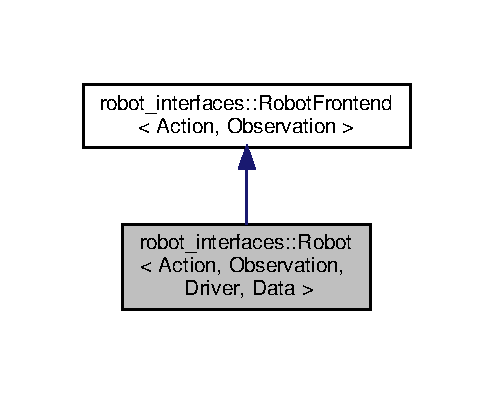
\includegraphics[width=237pt]{classrobot__interfaces_1_1Robot__coll__graph}
\end{center}
\end{figure}
\subsection*{Public Member Functions}
\begin{DoxyCompactItemize}
\item 
{\footnotesize template$<$typename... Args$>$ }\\\hyperlink{classrobot__interfaces_1_1Robot_ad91be1a022f648a691de55202f58543e}{Robot} (double max\+\_\+action\+\_\+duration\+\_\+s, double max\+\_\+inter\+\_\+action\+\_\+duration\+\_\+s, Args... args)
\item 
{\footnotesize template$<$typename... Args$>$ }\\\hyperlink{classrobot__interfaces_1_1Robot_a2db649f1bb6951f30111e0d35b760407}{Robot} (Args... args)
\begin{DoxyCompactList}\small\item\em \hyperlink{classrobot__interfaces_1_1Robot}{Robot} which instantiates a non real time mode backend. \end{DoxyCompactList}\item 
\mbox{\Hypertarget{classrobot__interfaces_1_1Robot_af2d47a88a06f94e90bc0145ba1171cd0}\label{classrobot__interfaces_1_1Robot_af2d47a88a06f94e90bc0145ba1171cd0}} 
void \hyperlink{classrobot__interfaces_1_1Robot_af2d47a88a06f94e90bc0145ba1171cd0}{initialize} ()
\begin{DoxyCompactList}\small\item\em initialize the backend \end{DoxyCompactList}\item 
\mbox{\Hypertarget{classrobot__interfaces_1_1Robot_af6e817bb62ff3d22ce1a9353709818c3}\label{classrobot__interfaces_1_1Robot_af6e817bb62ff3d22ce1a9353709818c3}} 
const Data \& \hyperlink{classrobot__interfaces_1_1Robot_af6e817bb62ff3d22ce1a9353709818c3}{get\+\_\+data} () const
\begin{DoxyCompactList}\small\item\em return the data shared by the frontend and the backend. \end{DoxyCompactList}\end{DoxyCompactItemize}
\subsection*{Private Types}
\begin{DoxyCompactItemize}
\item 
\mbox{\Hypertarget{classrobot__interfaces_1_1Robot_aae6cdfcef2853a056a6f7d7d2356b7df}\label{classrobot__interfaces_1_1Robot_aae6cdfcef2853a056a6f7d7d2356b7df}} 
typedef std\+::shared\+\_\+ptr$<$ Data $>$ {\bfseries Data\+Ptr}
\item 
\mbox{\Hypertarget{classrobot__interfaces_1_1Robot_a8aa32d96551cdd9234288203b1790f6d}\label{classrobot__interfaces_1_1Robot_a8aa32d96551cdd9234288203b1790f6d}} 
typedef std\+::shared\+\_\+ptr$<$ \hyperlink{classDriver}{Driver} $>$ {\bfseries Robot\+Driver\+Ptr}
\end{DoxyCompactItemize}
\subsection*{Private Attributes}
\begin{DoxyCompactItemize}
\item 
\mbox{\Hypertarget{classrobot__interfaces_1_1Robot_add04574720fb6d4ecc9fd74678b3627e}\label{classrobot__interfaces_1_1Robot_add04574720fb6d4ecc9fd74678b3627e}} 
Robot\+Driver\+Ptr {\bfseries driver\+\_\+ptr\+\_\+}
\item 
\mbox{\Hypertarget{classrobot__interfaces_1_1Robot_abefd57cd42aad6c21b3db990d4488db4}\label{classrobot__interfaces_1_1Robot_abefd57cd42aad6c21b3db990d4488db4}} 
\hyperlink{classrobot__interfaces_1_1RobotBackend}{Robot\+Backend}$<$ Action, Observation $>$ {\bfseries backend\+\_\+}
\end{DoxyCompactItemize}
\subsection*{Additional Inherited Members}


\subsection{Detailed Description}
\subsubsection*{template$<$typename Action, typename Observation, typename Driver, typename Data = Single\+Process\+Robot\+Data$<$\+Action, Observation$>$$>$\newline
class robot\+\_\+interfaces\+::\+Robot$<$ Action, Observation, Driver, Data $>$}

\hyperlink{classrobot__interfaces_1_1RobotFrontend}{Robot\+Frontend} that construct and encapsulates its related \hyperlink{classrobot__interfaces_1_1RobotBackend}{Robot\+Backend}. 

It also construct and starts the robot driver. \begin{Desc}
\item[Examples\+: ]\par
\hyperlink{demo_8cpp-example}{demo.\+cpp}.\end{Desc}


\subsection{Constructor \& Destructor Documentation}
\mbox{\Hypertarget{classrobot__interfaces_1_1Robot_ad91be1a022f648a691de55202f58543e}\label{classrobot__interfaces_1_1Robot_ad91be1a022f648a691de55202f58543e}} 
\index{robot\+\_\+interfaces\+::\+Robot@{robot\+\_\+interfaces\+::\+Robot}!Robot@{Robot}}
\index{Robot@{Robot}!robot\+\_\+interfaces\+::\+Robot@{robot\+\_\+interfaces\+::\+Robot}}
\subsubsection{\texorpdfstring{Robot()}{Robot()}\hspace{0.1cm}{\footnotesize\ttfamily [1/2]}}
{\footnotesize\ttfamily template$<$typename Action , typename Observation , typename Driver , typename Data  = Single\+Process\+Robot\+Data$<$\+Action, Observation$>$$>$ \\
template$<$typename... Args$>$ \\
\hyperlink{classrobot__interfaces_1_1Robot}{robot\+\_\+interfaces\+::\+Robot}$<$ Action, Observation, \hyperlink{classDriver}{Driver}, Data $>$\+::\hyperlink{classrobot__interfaces_1_1Robot}{Robot} (\begin{DoxyParamCaption}\item[{double}]{max\+\_\+action\+\_\+duration\+\_\+s,  }\item[{double}]{max\+\_\+inter\+\_\+action\+\_\+duration\+\_\+s,  }\item[{Args...}]{args }\end{DoxyParamCaption})\hspace{0.3cm}{\ttfamily [inline]}}


\begin{DoxyParams}{Parameters}
{\em max\+\_\+action\+\_\+duration\+\_\+s} & See \hyperlink{classrobot__interfaces_1_1MonitoredRobotDriver}{Monitored\+Robot\+Driver}. \\
\hline
{\em max\+\_\+inter\+\_\+action\+\_\+duration\+\_\+s} & See \hyperlink{classrobot__interfaces_1_1MonitoredRobotDriver}{Monitored\+Robot\+Driver}. \\
\hline
{\em args} & Arguments for instantiating \hyperlink{classDriver}{Driver} \\
\hline
\end{DoxyParams}
\mbox{\Hypertarget{classrobot__interfaces_1_1Robot_a2db649f1bb6951f30111e0d35b760407}\label{classrobot__interfaces_1_1Robot_a2db649f1bb6951f30111e0d35b760407}} 
\index{robot\+\_\+interfaces\+::\+Robot@{robot\+\_\+interfaces\+::\+Robot}!Robot@{Robot}}
\index{Robot@{Robot}!robot\+\_\+interfaces\+::\+Robot@{robot\+\_\+interfaces\+::\+Robot}}
\subsubsection{\texorpdfstring{Robot()}{Robot()}\hspace{0.1cm}{\footnotesize\ttfamily [2/2]}}
{\footnotesize\ttfamily template$<$typename Action , typename Observation , typename Driver , typename Data  = Single\+Process\+Robot\+Data$<$\+Action, Observation$>$$>$ \\
template$<$typename... Args$>$ \\
\hyperlink{classrobot__interfaces_1_1Robot}{robot\+\_\+interfaces\+::\+Robot}$<$ Action, Observation, \hyperlink{classDriver}{Driver}, Data $>$\+::\hyperlink{classrobot__interfaces_1_1Robot}{Robot} (\begin{DoxyParamCaption}\item[{Args...}]{args }\end{DoxyParamCaption})\hspace{0.3cm}{\ttfamily [inline]}}



\hyperlink{classrobot__interfaces_1_1Robot}{Robot} which instantiates a non real time mode backend. 


\begin{DoxyParams}{Parameters}
{\em max\+\_\+action\+\_\+duration\+\_\+s} & See \hyperlink{classrobot__interfaces_1_1MonitoredRobotDriver}{Monitored\+Robot\+Driver}. \\
\hline
{\em max\+\_\+inter\+\_\+action\+\_\+duration\+\_\+s} & See \hyperlink{classrobot__interfaces_1_1MonitoredRobotDriver}{Monitored\+Robot\+Driver}. \\
\hline
{\em args} & Arguments for instantiating \hyperlink{classDriver}{Driver} \\
\hline
\end{DoxyParams}


The documentation for this class was generated from the following file\+:\begin{DoxyCompactItemize}
\item 
include/robot\+\_\+interfaces/robot.\+hpp\end{DoxyCompactItemize}

\hypertarget{classrobot__interfaces_1_1RobotBackend}{}\section{robot\+\_\+interfaces\+:\+:Robot\+Backend$<$ Action, Observation $>$ Class Template Reference}
\label{classrobot__interfaces_1_1RobotBackend}\index{robot\+\_\+interfaces\+::\+Robot\+Backend$<$ Action, Observation $>$@{robot\+\_\+interfaces\+::\+Robot\+Backend$<$ Action, Observation $>$}}


Communication link between \hyperlink{classrobot__interfaces_1_1RobotDriver}{Robot\+Driver} and \hyperlink{classrobot__interfaces_1_1RobotData}{Robot\+Data}.  




{\ttfamily \#include $<$robot\+\_\+backend.\+hpp$>$}

\subsection*{Public Member Functions}
\begin{DoxyCompactItemize}
\item 
\hyperlink{classrobot__interfaces_1_1RobotBackend_af454a09b5d269ed32b0ae2d35abdb833}{Robot\+Backend} (std\+::shared\+\_\+ptr$<$ \hyperlink{classrobot__interfaces_1_1RobotDriver}{Robot\+Driver}$<$ Action, Observation $>$$>$ robot\+\_\+driver, std\+::shared\+\_\+ptr$<$ \hyperlink{classrobot__interfaces_1_1RobotData}{Robot\+Data}$<$ Action, Observation $>$$>$ robot\+\_\+data, const bool real\+\_\+time\+\_\+mode=true, const double first\+\_\+action\+\_\+timeout=std\+::numeric\+\_\+limits$<$ double $>$\+::infinity(), const uint32\+\_\+t max\+\_\+number\+\_\+of\+\_\+actions=0)
\item 
\mbox{\Hypertarget{classrobot__interfaces_1_1RobotBackend_ae354dfd960d4fd0d2f9242dcfb4a701f}\label{classrobot__interfaces_1_1RobotBackend_ae354dfd960d4fd0d2f9242dcfb4a701f}} 
uint32\+\_\+t {\bfseries get\+\_\+max\+\_\+action\+\_\+repetitions} ()
\item 
void \hyperlink{classrobot__interfaces_1_1RobotBackend_aad761d1e0ab7296a9632b9c4cc9c91db}{set\+\_\+max\+\_\+action\+\_\+repetitions} (const uint32\+\_\+t \&max\+\_\+action\+\_\+repetitions)
\begin{DoxyCompactList}\small\item\em Set how often an action is repeated if no new one is provided. \end{DoxyCompactList}\item 
\mbox{\Hypertarget{classrobot__interfaces_1_1RobotBackend_a7e4eb9f5362b79c0c21b824e3b639ae6}\label{classrobot__interfaces_1_1RobotBackend_a7e4eb9f5362b79c0c21b824e3b639ae6}} 
void {\bfseries initialize} ()
\item 
void \hyperlink{classrobot__interfaces_1_1RobotBackend_a3da1748227b56acf7b745aff64023715}{request\+\_\+shutdown} ()
\begin{DoxyCompactList}\small\item\em Request shutdown of the backend loop. \end{DoxyCompactList}\item 
\mbox{\Hypertarget{classrobot__interfaces_1_1RobotBackend_ad4e9c9fda8d3bbab60b1896df1e1e78b}\label{classrobot__interfaces_1_1RobotBackend_ad4e9c9fda8d3bbab60b1896df1e1e78b}} 
void \hyperlink{classrobot__interfaces_1_1RobotBackend_ad4e9c9fda8d3bbab60b1896df1e1e78b}{wait\+\_\+until\+\_\+terminated} () const
\begin{DoxyCompactList}\small\item\em Wait until the backend loop terminates. \end{DoxyCompactList}\end{DoxyCompactItemize}
\subsection*{Private Member Functions}
\begin{DoxyCompactItemize}
\item 
\mbox{\Hypertarget{classrobot__interfaces_1_1RobotBackend_acfbf64755fc1910ca26f441085c99225}\label{classrobot__interfaces_1_1RobotBackend_acfbf64755fc1910ca26f441085c99225}} 
bool {\bfseries has\+\_\+shutdown\+\_\+request} () const
\item 
void \hyperlink{classrobot__interfaces_1_1RobotBackend_a7cc66183743f277c41614a44fcc47b1a}{loop} ()
\begin{DoxyCompactList}\small\item\em Main loop. \end{DoxyCompactList}\end{DoxyCompactItemize}
\subsection*{Static Private Member Functions}
\begin{DoxyCompactItemize}
\item 
\mbox{\Hypertarget{classrobot__interfaces_1_1RobotBackend_a44f21ab5414ea7742e34a3cf3dfe0650}\label{classrobot__interfaces_1_1RobotBackend_a44f21ab5414ea7742e34a3cf3dfe0650}} 
static void $\ast$ {\bfseries loop} (void $\ast$instance\+\_\+pointer)
\end{DoxyCompactItemize}
\subsection*{Private Attributes}
\begin{DoxyCompactItemize}
\item 
\mbox{\Hypertarget{classrobot__interfaces_1_1RobotBackend_a9c07b9b4a8c98b3f1b63d0754cbcb85b}\label{classrobot__interfaces_1_1RobotBackend_a9c07b9b4a8c98b3f1b63d0754cbcb85b}} 
std\+::shared\+\_\+ptr$<$ \hyperlink{classrobot__interfaces_1_1RobotDriver}{Robot\+Driver}$<$ Action, Observation $>$ $>$ {\bfseries robot\+\_\+driver\+\_\+}
\item 
\mbox{\Hypertarget{classrobot__interfaces_1_1RobotBackend_a4bb04e584d971d4d99a32ea8c5b0cd68}\label{classrobot__interfaces_1_1RobotBackend_a4bb04e584d971d4d99a32ea8c5b0cd68}} 
std\+::shared\+\_\+ptr$<$ \hyperlink{classrobot__interfaces_1_1RobotData}{Robot\+Data}$<$ Action, Observation $>$ $>$ {\bfseries robot\+\_\+data\+\_\+}
\item 
const bool \hyperlink{classrobot__interfaces_1_1RobotBackend_a81610183c52c9fe2088304bbd3b6f83f}{real\+\_\+time\+\_\+mode\+\_\+}
\begin{DoxyCompactList}\small\item\em Enable/disable real time mode. \end{DoxyCompactList}\item 
const double \hyperlink{classrobot__interfaces_1_1RobotBackend_a56f111a9e0663eedefbaf55de36f7cac}{first\+\_\+action\+\_\+timeout\+\_\+}
\begin{DoxyCompactList}\small\item\em Timeout for the first action to arrive. \end{DoxyCompactList}\item 
const uint32\+\_\+t \hyperlink{classrobot__interfaces_1_1RobotBackend_a7cac555549bff96a32da042a97919d47}{max\+\_\+number\+\_\+of\+\_\+actions\+\_\+}
\begin{DoxyCompactList}\small\item\em Maximum number of actions that are executed by the backend. \end{DoxyCompactList}\item 
std\+::atomic$<$ bool $>$ \hyperlink{classrobot__interfaces_1_1RobotBackend_abe24206dcf102b33f8ee472e287f485a}{is\+\_\+shutdown\+\_\+requested\+\_\+}
\begin{DoxyCompactList}\small\item\em Set to true when shutdown is requested. \end{DoxyCompactList}\item 
\mbox{\Hypertarget{classrobot__interfaces_1_1RobotBackend_a0e91800b352b7b52f22820775b1d5e99}\label{classrobot__interfaces_1_1RobotBackend_a0e91800b352b7b52f22820775b1d5e99}} 
std\+::atomic$<$ bool $>$ \hyperlink{classrobot__interfaces_1_1RobotBackend_a0e91800b352b7b52f22820775b1d5e99}{loop\+\_\+is\+\_\+running\+\_\+}
\begin{DoxyCompactList}\small\item\em Indicates if the background loop is still running. \end{DoxyCompactList}\item 
\mbox{\Hypertarget{classrobot__interfaces_1_1RobotBackend_ae40ecdc44212f79f96d63a84f7b8a6e8}\label{classrobot__interfaces_1_1RobotBackend_ae40ecdc44212f79f96d63a84f7b8a6e8}} 
uint32\+\_\+t \hyperlink{classrobot__interfaces_1_1RobotBackend_ae40ecdc44212f79f96d63a84f7b8a6e8}{max\+\_\+action\+\_\+repetitions\+\_\+}
\begin{DoxyCompactList}\small\item\em Number of times the previous action is repeated if no new one is provided. \end{DoxyCompactList}\item 
\mbox{\Hypertarget{classrobot__interfaces_1_1RobotBackend_a69c9b7f07651484d1677121f72832482}\label{classrobot__interfaces_1_1RobotBackend_a69c9b7f07651484d1677121f72832482}} 
real\+\_\+time\+\_\+tools\+::\+Checkpoint\+Timer$<$ 6, false $>$ {\bfseries timer\+\_\+}
\item 
\mbox{\Hypertarget{classrobot__interfaces_1_1RobotBackend_afcf4f2443b7f3000cece9b0851284717}\label{classrobot__interfaces_1_1RobotBackend_afcf4f2443b7f3000cece9b0851284717}} 
std\+::shared\+\_\+ptr$<$ real\+\_\+time\+\_\+tools\+::\+Real\+Time\+Thread $>$ {\bfseries thread\+\_\+}
\end{DoxyCompactItemize}


\subsection{Detailed Description}
\subsubsection*{template$<$typename Action, typename Observation$>$\newline
class robot\+\_\+interfaces\+::\+Robot\+Backend$<$ Action, Observation $>$}

Communication link between \hyperlink{classrobot__interfaces_1_1RobotDriver}{Robot\+Driver} and \hyperlink{classrobot__interfaces_1_1RobotData}{Robot\+Data}. 

At each time-\/step, it gets the observation from the \hyperlink{classrobot__interfaces_1_1RobotDriver}{Robot\+Driver} and writes it to \hyperlink{classrobot__interfaces_1_1RobotData}{Robot\+Data}, and it takes the desired\+\_\+action from \hyperlink{classrobot__interfaces_1_1RobotData}{Robot\+Data} and applies it on the \hyperlink{classrobot__interfaces_1_1RobotDriver}{Robot\+Driver}.


\begin{DoxyTemplParams}{Template Parameters}
{\em Action} & \\
\hline
{\em Observation} & \\
\hline
\end{DoxyTemplParams}
\begin{Desc}
\item[Examples\+: ]\par
\hyperlink{demo_8cpp-example}{demo.\+cpp}, and \hyperlink{demo_multiprocess_backend_8cpp-example}{demo\+\_\+multiprocess\+\_\+backend.\+cpp}.\end{Desc}


\subsection{Constructor \& Destructor Documentation}
\mbox{\Hypertarget{classrobot__interfaces_1_1RobotBackend_af454a09b5d269ed32b0ae2d35abdb833}\label{classrobot__interfaces_1_1RobotBackend_af454a09b5d269ed32b0ae2d35abdb833}} 
\index{robot\+\_\+interfaces\+::\+Robot\+Backend@{robot\+\_\+interfaces\+::\+Robot\+Backend}!Robot\+Backend@{Robot\+Backend}}
\index{Robot\+Backend@{Robot\+Backend}!robot\+\_\+interfaces\+::\+Robot\+Backend@{robot\+\_\+interfaces\+::\+Robot\+Backend}}
\subsubsection{\texorpdfstring{Robot\+Backend()}{RobotBackend()}}
{\footnotesize\ttfamily template$<$typename Action, typename Observation$>$ \\
\hyperlink{classrobot__interfaces_1_1RobotBackend}{robot\+\_\+interfaces\+::\+Robot\+Backend}$<$ Action, Observation $>$\+::\hyperlink{classrobot__interfaces_1_1RobotBackend}{Robot\+Backend} (\begin{DoxyParamCaption}\item[{std\+::shared\+\_\+ptr$<$ \hyperlink{classrobot__interfaces_1_1RobotDriver}{Robot\+Driver}$<$ Action, Observation $>$$>$}]{robot\+\_\+driver,  }\item[{std\+::shared\+\_\+ptr$<$ \hyperlink{classrobot__interfaces_1_1RobotData}{Robot\+Data}$<$ Action, Observation $>$$>$}]{robot\+\_\+data,  }\item[{const bool}]{real\+\_\+time\+\_\+mode = {\ttfamily true},  }\item[{const double}]{first\+\_\+action\+\_\+timeout = {\ttfamily std\+:\+:numeric\+\_\+limits$<$double$>$\+:\+:infinity()},  }\item[{const uint32\+\_\+t}]{max\+\_\+number\+\_\+of\+\_\+actions = {\ttfamily 0} }\end{DoxyParamCaption})\hspace{0.3cm}{\ttfamily [inline]}}


\begin{DoxyParams}{Parameters}
{\em robot\+\_\+driver} & \hyperlink{classDriver}{Driver} instance for the actual robot. \\
\hline
{\em robot\+\_\+data} & Data is send to/retrieved from here. \\
\hline
{\em real\+\_\+time\+\_\+mode} & Enable/disable real-\/time mode. In real-\/time mode, the backend will repeat previous actions if the new one is not provided in time or fail with an error if the allowed number of repetitions is exceeded. In non-\/real-\/time mode, it will simply block and wait until the action is provided. \\
\hline
{\em first\+\_\+action\+\_\+timeout} & See \hyperlink{classrobot__interfaces_1_1RobotBackend_a56f111a9e0663eedefbaf55de36f7cac}{Robot\+Backend\+::first\+\_\+action\+\_\+timeout\+\_\+}. \\
\hline
{\em max\+\_\+number\+\_\+of\+\_\+actions} & See \hyperlink{classrobot__interfaces_1_1RobotBackend_a7cac555549bff96a32da042a97919d47}{Robot\+Backend\+::max\+\_\+number\+\_\+of\+\_\+actions\+\_\+}. \\
\hline
\end{DoxyParams}


\subsection{Member Function Documentation}
\mbox{\Hypertarget{classrobot__interfaces_1_1RobotBackend_a7cc66183743f277c41614a44fcc47b1a}\label{classrobot__interfaces_1_1RobotBackend_a7cc66183743f277c41614a44fcc47b1a}} 
\index{robot\+\_\+interfaces\+::\+Robot\+Backend@{robot\+\_\+interfaces\+::\+Robot\+Backend}!loop@{loop}}
\index{loop@{loop}!robot\+\_\+interfaces\+::\+Robot\+Backend@{robot\+\_\+interfaces\+::\+Robot\+Backend}}
\subsubsection{\texorpdfstring{loop()}{loop()}}
{\footnotesize\ttfamily template$<$typename Action, typename Observation$>$ \\
void \hyperlink{classrobot__interfaces_1_1RobotBackend}{robot\+\_\+interfaces\+::\+Robot\+Backend}$<$ Action, Observation $>$\+::loop (\begin{DoxyParamCaption}{ }\end{DoxyParamCaption})\hspace{0.3cm}{\ttfamily [inline]}, {\ttfamily [private]}}



Main loop. 

Iterate over robot\+\_\+data\+\_\+.\+desired\+\_\+action and apply these actions to the robot, and read the applied\+\_\+action and the observation from the robot and append them to the corresponding timeseries in robot\+\_\+data\+\_\+. \mbox{\Hypertarget{classrobot__interfaces_1_1RobotBackend_a3da1748227b56acf7b745aff64023715}\label{classrobot__interfaces_1_1RobotBackend_a3da1748227b56acf7b745aff64023715}} 
\index{robot\+\_\+interfaces\+::\+Robot\+Backend@{robot\+\_\+interfaces\+::\+Robot\+Backend}!request\+\_\+shutdown@{request\+\_\+shutdown}}
\index{request\+\_\+shutdown@{request\+\_\+shutdown}!robot\+\_\+interfaces\+::\+Robot\+Backend@{robot\+\_\+interfaces\+::\+Robot\+Backend}}
\subsubsection{\texorpdfstring{request\+\_\+shutdown()}{request\_shutdown()}}
{\footnotesize\ttfamily template$<$typename Action, typename Observation$>$ \\
void \hyperlink{classrobot__interfaces_1_1RobotBackend}{robot\+\_\+interfaces\+::\+Robot\+Backend}$<$ Action, Observation $>$\+::request\+\_\+shutdown (\begin{DoxyParamCaption}{ }\end{DoxyParamCaption})\hspace{0.3cm}{\ttfamily [inline]}}



Request shutdown of the backend loop. 

The loop may take some time to actually terminate after calling this function. Use \hyperlink{classrobot__interfaces_1_1RobotBackend_ad4e9c9fda8d3bbab60b1896df1e1e78b}{wait\+\_\+until\+\_\+terminated()} to ensure it has really terminated. \mbox{\Hypertarget{classrobot__interfaces_1_1RobotBackend_aad761d1e0ab7296a9632b9c4cc9c91db}\label{classrobot__interfaces_1_1RobotBackend_aad761d1e0ab7296a9632b9c4cc9c91db}} 
\index{robot\+\_\+interfaces\+::\+Robot\+Backend@{robot\+\_\+interfaces\+::\+Robot\+Backend}!set\+\_\+max\+\_\+action\+\_\+repetitions@{set\+\_\+max\+\_\+action\+\_\+repetitions}}
\index{set\+\_\+max\+\_\+action\+\_\+repetitions@{set\+\_\+max\+\_\+action\+\_\+repetitions}!robot\+\_\+interfaces\+::\+Robot\+Backend@{robot\+\_\+interfaces\+::\+Robot\+Backend}}
\subsubsection{\texorpdfstring{set\+\_\+max\+\_\+action\+\_\+repetitions()}{set\_max\_action\_repetitions()}}
{\footnotesize\ttfamily template$<$typename Action, typename Observation$>$ \\
void \hyperlink{classrobot__interfaces_1_1RobotBackend}{robot\+\_\+interfaces\+::\+Robot\+Backend}$<$ Action, Observation $>$\+::set\+\_\+max\+\_\+action\+\_\+repetitions (\begin{DoxyParamCaption}\item[{const uint32\+\_\+t \&}]{max\+\_\+action\+\_\+repetitions }\end{DoxyParamCaption})\hspace{0.3cm}{\ttfamily [inline]}}



Set how often an action is repeated if no new one is provided. 

If the next action is due to be executed but the user did not provide one yet (i.\+e. there is no new action in the robot data time series), the last action will be repeated by automatically adding it to the time series again.

Use this this method to specify how often the action shall be repeated (default is 0, i.\+e. no repetition at all). If this limit is exceeded, the robot will be shut down and the \hyperlink{classrobot__interfaces_1_1RobotBackend}{Robot\+Backend} stops.

{\bfseries Note\+:} This is ignored in non-\/real-\/time mode.


\begin{DoxyParams}{Parameters}
{\em max\+\_\+action\+\_\+repetitions} & \\
\hline
\end{DoxyParams}


\subsection{Member Data Documentation}
\mbox{\Hypertarget{classrobot__interfaces_1_1RobotBackend_a56f111a9e0663eedefbaf55de36f7cac}\label{classrobot__interfaces_1_1RobotBackend_a56f111a9e0663eedefbaf55de36f7cac}} 
\index{robot\+\_\+interfaces\+::\+Robot\+Backend@{robot\+\_\+interfaces\+::\+Robot\+Backend}!first\+\_\+action\+\_\+timeout\+\_\+@{first\+\_\+action\+\_\+timeout\+\_\+}}
\index{first\+\_\+action\+\_\+timeout\+\_\+@{first\+\_\+action\+\_\+timeout\+\_\+}!robot\+\_\+interfaces\+::\+Robot\+Backend@{robot\+\_\+interfaces\+::\+Robot\+Backend}}
\subsubsection{\texorpdfstring{first\+\_\+action\+\_\+timeout\+\_\+}{first\_action\_timeout\_}}
{\footnotesize\ttfamily template$<$typename Action, typename Observation$>$ \\
const double \hyperlink{classrobot__interfaces_1_1RobotBackend}{robot\+\_\+interfaces\+::\+Robot\+Backend}$<$ Action, Observation $>$\+::first\+\_\+action\+\_\+timeout\+\_\+\hspace{0.3cm}{\ttfamily [private]}}



Timeout for the first action to arrive. 

Timeout for the time between starting the backend loop and receiving the first action from the user. If exceeded, the backend shuts down. Set to infinity to disable the timeout. \mbox{\Hypertarget{classrobot__interfaces_1_1RobotBackend_abe24206dcf102b33f8ee472e287f485a}\label{classrobot__interfaces_1_1RobotBackend_abe24206dcf102b33f8ee472e287f485a}} 
\index{robot\+\_\+interfaces\+::\+Robot\+Backend@{robot\+\_\+interfaces\+::\+Robot\+Backend}!is\+\_\+shutdown\+\_\+requested\+\_\+@{is\+\_\+shutdown\+\_\+requested\+\_\+}}
\index{is\+\_\+shutdown\+\_\+requested\+\_\+@{is\+\_\+shutdown\+\_\+requested\+\_\+}!robot\+\_\+interfaces\+::\+Robot\+Backend@{robot\+\_\+interfaces\+::\+Robot\+Backend}}
\subsubsection{\texorpdfstring{is\+\_\+shutdown\+\_\+requested\+\_\+}{is\_shutdown\_requested\_}}
{\footnotesize\ttfamily template$<$typename Action, typename Observation$>$ \\
std\+::atomic$<$bool$>$ \hyperlink{classrobot__interfaces_1_1RobotBackend}{robot\+\_\+interfaces\+::\+Robot\+Backend}$<$ Action, Observation $>$\+::is\+\_\+shutdown\+\_\+requested\+\_\+\hspace{0.3cm}{\ttfamily [private]}}



Set to true when shutdown is requested. 

This is used to notify the background loop about requested shutdown, so it terminates itself. \mbox{\Hypertarget{classrobot__interfaces_1_1RobotBackend_a7cac555549bff96a32da042a97919d47}\label{classrobot__interfaces_1_1RobotBackend_a7cac555549bff96a32da042a97919d47}} 
\index{robot\+\_\+interfaces\+::\+Robot\+Backend@{robot\+\_\+interfaces\+::\+Robot\+Backend}!max\+\_\+number\+\_\+of\+\_\+actions\+\_\+@{max\+\_\+number\+\_\+of\+\_\+actions\+\_\+}}
\index{max\+\_\+number\+\_\+of\+\_\+actions\+\_\+@{max\+\_\+number\+\_\+of\+\_\+actions\+\_\+}!robot\+\_\+interfaces\+::\+Robot\+Backend@{robot\+\_\+interfaces\+::\+Robot\+Backend}}
\subsubsection{\texorpdfstring{max\+\_\+number\+\_\+of\+\_\+actions\+\_\+}{max\_number\_of\_actions\_}}
{\footnotesize\ttfamily template$<$typename Action, typename Observation$>$ \\
const uint32\+\_\+t \hyperlink{classrobot__interfaces_1_1RobotBackend}{robot\+\_\+interfaces\+::\+Robot\+Backend}$<$ Action, Observation $>$\+::max\+\_\+number\+\_\+of\+\_\+actions\+\_\+\hspace{0.3cm}{\ttfamily [private]}}



Maximum number of actions that are executed by the backend. 

If set to a value greater than zero, the backend will automatically shut down after the specified number of actions is executed. \mbox{\Hypertarget{classrobot__interfaces_1_1RobotBackend_a81610183c52c9fe2088304bbd3b6f83f}\label{classrobot__interfaces_1_1RobotBackend_a81610183c52c9fe2088304bbd3b6f83f}} 
\index{robot\+\_\+interfaces\+::\+Robot\+Backend@{robot\+\_\+interfaces\+::\+Robot\+Backend}!real\+\_\+time\+\_\+mode\+\_\+@{real\+\_\+time\+\_\+mode\+\_\+}}
\index{real\+\_\+time\+\_\+mode\+\_\+@{real\+\_\+time\+\_\+mode\+\_\+}!robot\+\_\+interfaces\+::\+Robot\+Backend@{robot\+\_\+interfaces\+::\+Robot\+Backend}}
\subsubsection{\texorpdfstring{real\+\_\+time\+\_\+mode\+\_\+}{real\_time\_mode\_}}
{\footnotesize\ttfamily template$<$typename Action, typename Observation$>$ \\
const bool \hyperlink{classrobot__interfaces_1_1RobotBackend}{robot\+\_\+interfaces\+::\+Robot\+Backend}$<$ Action, Observation $>$\+::real\+\_\+time\+\_\+mode\+\_\+\hspace{0.3cm}{\ttfamily [private]}}



Enable/disable real time mode. 

If real time mode is enabled (true), the back end expects new actions to be provided in time by the user. If this does not happen, the last received action is repeated until the configured number of repetitions is exceeded in which case it stops with an error.

If real time mode is disabled (false), the back-\/end loop blocks and waits for the next action if it is not provided in time.

\begin{DoxySeeAlso}{See also}
\hyperlink{classrobot__interfaces_1_1RobotBackend_ae40ecdc44212f79f96d63a84f7b8a6e8}{max\+\_\+action\+\_\+repetitions\+\_\+} 
\end{DoxySeeAlso}


The documentation for this class was generated from the following file\+:\begin{DoxyCompactItemize}
\item 
include/robot\+\_\+interfaces/robot\+\_\+backend.\+hpp\end{DoxyCompactItemize}

\hypertarget{classrobot__interfaces_1_1RobotData}{}\section{robot\+\_\+interfaces\+:\+:Robot\+Data$<$ Action, Observation $>$ Class Template Reference}
\label{classrobot__interfaces_1_1RobotData}\index{robot\+\_\+interfaces\+::\+Robot\+Data$<$ Action, Observation $>$@{robot\+\_\+interfaces\+::\+Robot\+Data$<$ Action, Observation $>$}}


Contains all the input and output data of the robot.  




{\ttfamily \#include $<$robot\+\_\+data.\+hpp$>$}



Inheritance diagram for robot\+\_\+interfaces\+:\+:Robot\+Data$<$ Action, Observation $>$\+:
\nopagebreak
\begin{figure}[H]
\begin{center}
\leavevmode
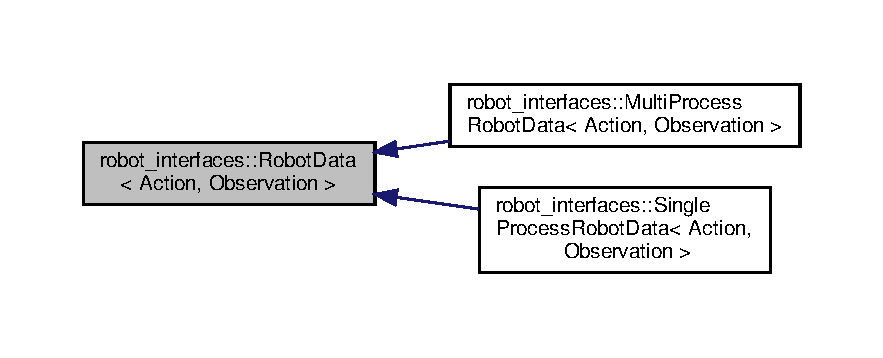
\includegraphics[width=350pt]{classrobot__interfaces_1_1RobotData__inherit__graph}
\end{center}
\end{figure}
\subsection*{Public Attributes}
\begin{DoxyCompactItemize}
\item 
\mbox{\Hypertarget{classrobot__interfaces_1_1RobotData_a03b4160b90de7eac5ffb67cb8a872cee}\label{classrobot__interfaces_1_1RobotData_a03b4160b90de7eac5ffb67cb8a872cee}} 
std\+::shared\+\_\+ptr$<$ time\+\_\+series\+::\+Time\+Series\+Interface$<$ Action $>$ $>$ \hyperlink{classrobot__interfaces_1_1RobotData_a03b4160b90de7eac5ffb67cb8a872cee}{desired\+\_\+action}
\begin{DoxyCompactList}\small\item\em Time series of the desired actions. \end{DoxyCompactList}\item 
\mbox{\Hypertarget{classrobot__interfaces_1_1RobotData_a05fea4d2f75f7fc34daf2bfc71fbfc4b}\label{classrobot__interfaces_1_1RobotData_a05fea4d2f75f7fc34daf2bfc71fbfc4b}} 
std\+::shared\+\_\+ptr$<$ time\+\_\+series\+::\+Time\+Series\+Interface$<$ Action $>$ $>$ \hyperlink{classrobot__interfaces_1_1RobotData_a05fea4d2f75f7fc34daf2bfc71fbfc4b}{applied\+\_\+action}
\begin{DoxyCompactList}\small\item\em Time series of the actually applied actions (due to safety. \end{DoxyCompactList}\item 
\mbox{\Hypertarget{classrobot__interfaces_1_1RobotData_ae3d13595b92f82f76b0f1df2961258bd}\label{classrobot__interfaces_1_1RobotData_ae3d13595b92f82f76b0f1df2961258bd}} 
std\+::shared\+\_\+ptr$<$ time\+\_\+series\+::\+Time\+Series\+Interface$<$ Observation $>$ $>$ \hyperlink{classrobot__interfaces_1_1RobotData_ae3d13595b92f82f76b0f1df2961258bd}{observation}
\begin{DoxyCompactList}\small\item\em Time series of the observations retrieved from the robot. \end{DoxyCompactList}\item 
\mbox{\Hypertarget{classrobot__interfaces_1_1RobotData_a47c53daf923c30981d15008e5134f648}\label{classrobot__interfaces_1_1RobotData_a47c53daf923c30981d15008e5134f648}} 
std\+::shared\+\_\+ptr$<$ time\+\_\+series\+::\+Time\+Series\+Interface$<$ \hyperlink{structrobot__interfaces_1_1Status}{Status} $>$ $>$ \hyperlink{classrobot__interfaces_1_1RobotData_a47c53daf923c30981d15008e5134f648}{status}
\begin{DoxyCompactList}\small\item\em Time series of status messages. \end{DoxyCompactList}\end{DoxyCompactItemize}


\subsection{Detailed Description}
\subsubsection*{template$<$typename Action, typename Observation$>$\newline
class robot\+\_\+interfaces\+::\+Robot\+Data$<$ Action, Observation $>$}

Contains all the input and output data of the robot. 

This means the
\begin{DoxyItemize}
\item {\ttfamily desired\+\_\+action} which was requested by the robot user
\item {\ttfamily applied\+\_\+action} which was actually applied and may not be and may not be identical to desired\+\_\+action for safety reasons
\item {\ttfamily observation} made by the robot
\item {\ttfamily status} which keeps track of timing issues and errors.
\end{DoxyItemize}

See this graph to understand how they relate to each other precisely in terms of time\+:

\begin{DoxyVerb}|------ t = 0 ------|------ t = 1 ------|
|----- action0 -----|----- action1 -----|
o                   o                   o
b                   b                   b
s                   s                   s
0                   1                   2
\end{DoxyVerb}



\begin{DoxyTemplParams}{Template Parameters}
{\em Action} & Type of the actions. \\
\hline
{\em Observation} & Type of the observations. \\
\hline
\end{DoxyTemplParams}


The documentation for this class was generated from the following file\+:\begin{DoxyCompactItemize}
\item 
include/robot\+\_\+interfaces/\hyperlink{robot__data_8hpp}{robot\+\_\+data.\+hpp}\end{DoxyCompactItemize}

\hypertarget{classrobot__interfaces_1_1RobotDriver}{}\section{robot\+\_\+interfaces\+:\+:Robot\+Driver$<$ T\+Action, T\+Observation $>$ Class Template Reference}
\label{classrobot__interfaces_1_1RobotDriver}\index{robot\+\_\+interfaces\+::\+Robot\+Driver$<$ T\+Action, T\+Observation $>$@{robot\+\_\+interfaces\+::\+Robot\+Driver$<$ T\+Action, T\+Observation $>$}}


\hyperlink{classDriver}{Driver} for interfacing the actual robot hardware or simulation.  




{\ttfamily \#include $<$robot\+\_\+driver.\+hpp$>$}

\subsection*{Public Types}
\begin{DoxyCompactItemize}
\item 
\mbox{\Hypertarget{classrobot__interfaces_1_1RobotDriver_acbba637e7857bef5c7a1e64c9846ead7}\label{classrobot__interfaces_1_1RobotDriver_acbba637e7857bef5c7a1e64c9846ead7}} 
typedef T\+Action {\bfseries Action}
\item 
\mbox{\Hypertarget{classrobot__interfaces_1_1RobotDriver_abcb094711d0ae09fd8e2fc9a6aa771f2}\label{classrobot__interfaces_1_1RobotDriver_abcb094711d0ae09fd8e2fc9a6aa771f2}} 
typedef T\+Observation {\bfseries Observation}
\end{DoxyCompactItemize}
\subsection*{Public Member Functions}
\begin{DoxyCompactItemize}
\item 
virtual void \hyperlink{classrobot__interfaces_1_1RobotDriver_af3cbef570a455e1f8085d701282264ff}{initialize} ()=0
\begin{DoxyCompactList}\small\item\em Initialize the robot. \end{DoxyCompactList}\item 
virtual Action \hyperlink{classrobot__interfaces_1_1RobotDriver_a4294e522fcd12b38d69f7d53fae5d74a}{apply\+\_\+action} (const Action \&desired\+\_\+action)=0
\begin{DoxyCompactList}\small\item\em Apply action immediately and block until it is executed. \end{DoxyCompactList}\item 
virtual Observation \hyperlink{classrobot__interfaces_1_1RobotDriver_ad13d4f4fdfe78bdde4fc964f07fa45e2}{get\+\_\+latest\+\_\+observation} ()=0
\begin{DoxyCompactList}\small\item\em Return the latest observation immediately. \end{DoxyCompactList}\item 
virtual std\+::string \hyperlink{classrobot__interfaces_1_1RobotDriver_acdf4c5d6993b836a180e6b6fc12b3445}{get\+\_\+error} ()=0
\begin{DoxyCompactList}\small\item\em Get error message if there is any error. \end{DoxyCompactList}\item 
virtual void \hyperlink{classrobot__interfaces_1_1RobotDriver_a3451fb8b15d2840b559f3ee858de01f8}{shutdown} ()=0
\begin{DoxyCompactList}\small\item\em Shut down the robot safely. \end{DoxyCompactList}\end{DoxyCompactItemize}


\subsection{Detailed Description}
\subsubsection*{template$<$typename T\+Action, typename T\+Observation$>$\newline
class robot\+\_\+interfaces\+::\+Robot\+Driver$<$ T\+Action, T\+Observation $>$}

\hyperlink{classDriver}{Driver} for interfacing the actual robot hardware or simulation. 

Interface to the robot used by the subsequent classes. Any robot (be it real or simulation) has to derive from this class and implement the functions \hyperlink{classrobot__interfaces_1_1RobotDriver_a4294e522fcd12b38d69f7d53fae5d74a}{apply\+\_\+action()}, \hyperlink{classrobot__interfaces_1_1RobotDriver_ad13d4f4fdfe78bdde4fc964f07fa45e2}{get\+\_\+latest\+\_\+observation()} and \hyperlink{classrobot__interfaces_1_1RobotDriver_a3451fb8b15d2840b559f3ee858de01f8}{shutdown()}. This Base class provides some timing logic around those three functions. It makes sure that after the first call of \hyperlink{classrobot__interfaces_1_1RobotDriver_a4294e522fcd12b38d69f7d53fae5d74a}{apply\+\_\+action()}, it is always called again after some specified time, otherwise the \hyperlink{classrobot__interfaces_1_1RobotDriver_a3451fb8b15d2840b559f3ee858de01f8}{shutdown()} method will be called. This Base class also makes sure that the \hyperlink{classrobot__interfaces_1_1RobotDriver_a4294e522fcd12b38d69f7d53fae5d74a}{apply\+\_\+action()} function itself does not take more time than expected.


\begin{DoxyTemplParams}{Template Parameters}
{\em Action} & \\
\hline
{\em Observation} & \\
\hline
\end{DoxyTemplParams}
\begin{Desc}
\item[Examples\+: ]\par
\hyperlink{demo_multiprocess_backend_8cpp-example}{demo\+\_\+multiprocess\+\_\+backend.\+cpp}.\end{Desc}


\subsection{Member Function Documentation}
\mbox{\Hypertarget{classrobot__interfaces_1_1RobotDriver_a4294e522fcd12b38d69f7d53fae5d74a}\label{classrobot__interfaces_1_1RobotDriver_a4294e522fcd12b38d69f7d53fae5d74a}} 
\index{robot\+\_\+interfaces\+::\+Robot\+Driver@{robot\+\_\+interfaces\+::\+Robot\+Driver}!apply\+\_\+action@{apply\+\_\+action}}
\index{apply\+\_\+action@{apply\+\_\+action}!robot\+\_\+interfaces\+::\+Robot\+Driver@{robot\+\_\+interfaces\+::\+Robot\+Driver}}
\subsubsection{\texorpdfstring{apply\+\_\+action()}{apply\_action()}}
{\footnotesize\ttfamily template$<$typename T\+Action, typename T\+Observation$>$ \\
virtual Action \hyperlink{classrobot__interfaces_1_1RobotDriver}{robot\+\_\+interfaces\+::\+Robot\+Driver}$<$ T\+Action, T\+Observation $>$\+::apply\+\_\+action (\begin{DoxyParamCaption}\item[{const Action \&}]{desired\+\_\+action }\end{DoxyParamCaption})\hspace{0.3cm}{\ttfamily [pure virtual]}}



Apply action immediately and block until it is executed. 

This method must apply the desired\+\_\+action immediately when it is called, and only return once the action has been executed completely. This way we can accommodate both simulators and real robots with this interface.


\begin{DoxyParams}{Parameters}
{\em desired\+\_\+action} & The action we want to apply. \\
\hline
\end{DoxyParams}
\begin{DoxyReturn}{Returns}
The action that was actually applied (since due to safety reasons it might not be possible to apply the desired action). 
\end{DoxyReturn}


Implemented in \hyperlink{classrobot__interfaces_1_1example_1_1Driver_aa18b1bc90441395e86794a90dfdac9fa}{robot\+\_\+interfaces\+::example\+::\+Driver}, and \hyperlink{classDriver_a0f8d51bef151ccc38a0cb7b226048e28}{Driver}.

\mbox{\Hypertarget{classrobot__interfaces_1_1RobotDriver_acdf4c5d6993b836a180e6b6fc12b3445}\label{classrobot__interfaces_1_1RobotDriver_acdf4c5d6993b836a180e6b6fc12b3445}} 
\index{robot\+\_\+interfaces\+::\+Robot\+Driver@{robot\+\_\+interfaces\+::\+Robot\+Driver}!get\+\_\+error@{get\+\_\+error}}
\index{get\+\_\+error@{get\+\_\+error}!robot\+\_\+interfaces\+::\+Robot\+Driver@{robot\+\_\+interfaces\+::\+Robot\+Driver}}
\subsubsection{\texorpdfstring{get\+\_\+error()}{get\_error()}}
{\footnotesize\ttfamily template$<$typename T\+Action, typename T\+Observation$>$ \\
virtual std\+::string \hyperlink{classrobot__interfaces_1_1RobotDriver}{robot\+\_\+interfaces\+::\+Robot\+Driver}$<$ T\+Action, T\+Observation $>$\+::get\+\_\+error (\begin{DoxyParamCaption}{ }\end{DoxyParamCaption})\hspace{0.3cm}{\ttfamily [pure virtual]}}



Get error message if there is any error. 

\begin{DoxyReturn}{Returns}
Returns an error message or an empty string if there is no error. 
\end{DoxyReturn}


Implemented in \hyperlink{classrobot__interfaces_1_1MonitoredRobotDriver_a944425cc7e0845184f33b16405a9e61e}{robot\+\_\+interfaces\+::\+Monitored\+Robot\+Driver$<$ Driver $>$}, \hyperlink{classrobot__interfaces_1_1example_1_1Driver_a8465b912da8f11a6db271f11ff4eced1}{robot\+\_\+interfaces\+::example\+::\+Driver}, and \hyperlink{classDriver_a6fb739b87c892c4102e838508855c0be}{Driver}.

\mbox{\Hypertarget{classrobot__interfaces_1_1RobotDriver_ad13d4f4fdfe78bdde4fc964f07fa45e2}\label{classrobot__interfaces_1_1RobotDriver_ad13d4f4fdfe78bdde4fc964f07fa45e2}} 
\index{robot\+\_\+interfaces\+::\+Robot\+Driver@{robot\+\_\+interfaces\+::\+Robot\+Driver}!get\+\_\+latest\+\_\+observation@{get\+\_\+latest\+\_\+observation}}
\index{get\+\_\+latest\+\_\+observation@{get\+\_\+latest\+\_\+observation}!robot\+\_\+interfaces\+::\+Robot\+Driver@{robot\+\_\+interfaces\+::\+Robot\+Driver}}
\subsubsection{\texorpdfstring{get\+\_\+latest\+\_\+observation()}{get\_latest\_observation()}}
{\footnotesize\ttfamily template$<$typename T\+Action, typename T\+Observation$>$ \\
virtual Observation \hyperlink{classrobot__interfaces_1_1RobotDriver}{robot\+\_\+interfaces\+::\+Robot\+Driver}$<$ T\+Action, T\+Observation $>$\+::get\+\_\+latest\+\_\+observation (\begin{DoxyParamCaption}{ }\end{DoxyParamCaption})\hspace{0.3cm}{\ttfamily [pure virtual]}}



Return the latest observation immediately. 

\begin{DoxyReturn}{Returns}
Observation 
\end{DoxyReturn}


Implemented in \hyperlink{classrobot__interfaces_1_1MonitoredRobotDriver_a97774dddcda1038f338d18ef0b572ad8}{robot\+\_\+interfaces\+::\+Monitored\+Robot\+Driver$<$ Driver $>$}, \hyperlink{classrobot__interfaces_1_1example_1_1Driver_a2fa7ee03258e65037ed69d9a8363bfe8}{robot\+\_\+interfaces\+::example\+::\+Driver}, and \hyperlink{classDriver_afb09663997bffc5c694fb5aa8aca243a}{Driver}.

\mbox{\Hypertarget{classrobot__interfaces_1_1RobotDriver_af3cbef570a455e1f8085d701282264ff}\label{classrobot__interfaces_1_1RobotDriver_af3cbef570a455e1f8085d701282264ff}} 
\index{robot\+\_\+interfaces\+::\+Robot\+Driver@{robot\+\_\+interfaces\+::\+Robot\+Driver}!initialize@{initialize}}
\index{initialize@{initialize}!robot\+\_\+interfaces\+::\+Robot\+Driver@{robot\+\_\+interfaces\+::\+Robot\+Driver}}
\subsubsection{\texorpdfstring{initialize()}{initialize()}}
{\footnotesize\ttfamily template$<$typename T\+Action, typename T\+Observation$>$ \\
virtual void \hyperlink{classrobot__interfaces_1_1RobotDriver}{robot\+\_\+interfaces\+::\+Robot\+Driver}$<$ T\+Action, T\+Observation $>$\+::initialize (\begin{DoxyParamCaption}{ }\end{DoxyParamCaption})\hspace{0.3cm}{\ttfamily [pure virtual]}}



Initialize the robot. 

Any initialization procedures that need to be done before sending actions to the robot should be done in this method (e.\+g. homing to find the absolute position). 

Implemented in \hyperlink{classrobot__interfaces_1_1MonitoredRobotDriver_a47b68c24afaa087e4e60e6413ab7ac89}{robot\+\_\+interfaces\+::\+Monitored\+Robot\+Driver$<$ Driver $>$}, \hyperlink{classrobot__interfaces_1_1example_1_1Driver_ab6f6c3f3ffb730d162bec70313f8aab7}{robot\+\_\+interfaces\+::example\+::\+Driver}, and \hyperlink{classDriver_a81c0beb523fad80cd40cfcc6a6e3de2d}{Driver}.

\mbox{\Hypertarget{classrobot__interfaces_1_1RobotDriver_a3451fb8b15d2840b559f3ee858de01f8}\label{classrobot__interfaces_1_1RobotDriver_a3451fb8b15d2840b559f3ee858de01f8}} 
\index{robot\+\_\+interfaces\+::\+Robot\+Driver@{robot\+\_\+interfaces\+::\+Robot\+Driver}!shutdown@{shutdown}}
\index{shutdown@{shutdown}!robot\+\_\+interfaces\+::\+Robot\+Driver@{robot\+\_\+interfaces\+::\+Robot\+Driver}}
\subsubsection{\texorpdfstring{shutdown()}{shutdown()}}
{\footnotesize\ttfamily template$<$typename T\+Action, typename T\+Observation$>$ \\
virtual void \hyperlink{classrobot__interfaces_1_1RobotDriver}{robot\+\_\+interfaces\+::\+Robot\+Driver}$<$ T\+Action, T\+Observation $>$\+::shutdown (\begin{DoxyParamCaption}{ }\end{DoxyParamCaption})\hspace{0.3cm}{\ttfamily [pure virtual]}}



Shut down the robot safely. 

Use this method if your robot needs to perform some action when shutting down, e.\+g. to move it to a defined rest position. 

Implemented in \hyperlink{classrobot__interfaces_1_1MonitoredRobotDriver_a95714a60e69a3ac06461382a7b391289}{robot\+\_\+interfaces\+::\+Monitored\+Robot\+Driver$<$ Driver $>$}, \hyperlink{classrobot__interfaces_1_1example_1_1Driver_a91cbe74896c9ed56ff7eee6380964dfe}{robot\+\_\+interfaces\+::example\+::\+Driver}, and \hyperlink{classDriver_a630fc9183eb419beb09b5828b4547b6d}{Driver}.



The documentation for this class was generated from the following file\+:\begin{DoxyCompactItemize}
\item 
include/robot\+\_\+interfaces/robot\+\_\+driver.\+hpp\end{DoxyCompactItemize}

\hypertarget{classrobot__interfaces_1_1RobotFrontend}{}\section{robot\+\_\+interfaces\+:\+:Robot\+Frontend$<$ Action, Observation $>$ Class Template Reference}
\label{classrobot__interfaces_1_1RobotFrontend}\index{robot\+\_\+interfaces\+::\+Robot\+Frontend$<$ Action, Observation $>$@{robot\+\_\+interfaces\+::\+Robot\+Frontend$<$ Action, Observation $>$}}


Communication link between \hyperlink{classrobot__interfaces_1_1RobotData}{Robot\+Data} and the user.  




{\ttfamily \#include $<$robot\+\_\+frontend.\+hpp$>$}



Inheritance diagram for robot\+\_\+interfaces\+:\+:Robot\+Frontend$<$ Action, Observation $>$\+:
\nopagebreak
\begin{figure}[H]
\begin{center}
\leavevmode
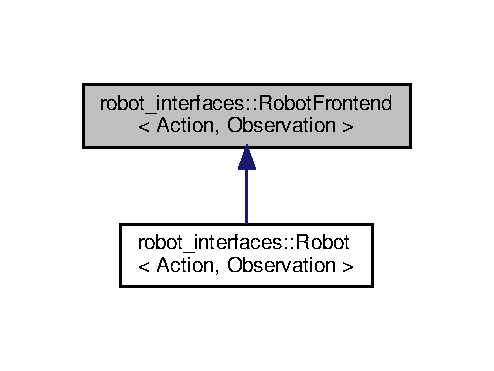
\includegraphics[width=237pt]{classrobot__interfaces_1_1RobotFrontend__inherit__graph}
\end{center}
\end{figure}
\subsection*{Public Types}
\begin{DoxyCompactItemize}
\item 
\mbox{\Hypertarget{classrobot__interfaces_1_1RobotFrontend_a02bebc6c3e9822f026c48f970d80a865}\label{classrobot__interfaces_1_1RobotFrontend_a02bebc6c3e9822f026c48f970d80a865}} 
typedef time\+\_\+series\+::\+Timestamp {\bfseries Time\+Stamp}
\end{DoxyCompactItemize}
\subsection*{Public Member Functions}
\begin{DoxyCompactItemize}
\item 
\mbox{\Hypertarget{classrobot__interfaces_1_1RobotFrontend_a0bd84764fb1a3004282706963aa48c3e}\label{classrobot__interfaces_1_1RobotFrontend_a0bd84764fb1a3004282706963aa48c3e}} 
{\bfseries Robot\+Frontend} (std\+::shared\+\_\+ptr$<$ \hyperlink{classrobot__interfaces_1_1RobotData}{Robot\+Data}$<$ Action, Observation $>$$>$ robot\+\_\+data)
\item 
Observation \hyperlink{classrobot__interfaces_1_1RobotFrontend_a95964f3d7aeaab7eec4c9a8782500c0f}{get\+\_\+observation} (const Time\+Index \&t) const
\begin{DoxyCompactList}\small\item\em Get observation of time step t. \end{DoxyCompactList}\item 
Action \hyperlink{classrobot__interfaces_1_1RobotFrontend_a8710ad1f0de000dfb099585e0ac7f140}{get\+\_\+desired\+\_\+action} (const Time\+Index \&t) const
\begin{DoxyCompactList}\small\item\em Get the desired action of time step t. \end{DoxyCompactList}\item 
Action \hyperlink{classrobot__interfaces_1_1RobotFrontend_a870651d849fe0f1a4909820cc3b6de40}{get\+\_\+applied\+\_\+action} (const Time\+Index \&t) const
\begin{DoxyCompactList}\small\item\em Get the applied action of time step t. \end{DoxyCompactList}\item 
\mbox{\Hypertarget{classrobot__interfaces_1_1RobotFrontend_a080a709a39ff710c2a38bd53ff313645}\label{classrobot__interfaces_1_1RobotFrontend_a080a709a39ff710c2a38bd53ff313645}} 
\hyperlink{structrobot__interfaces_1_1Status}{Status} {\bfseries get\+\_\+status} (const Time\+Index \&t) const
\item 
Time\+Stamp \hyperlink{classrobot__interfaces_1_1RobotFrontend_a68cfe3df122ae9fe5cc6ea15ea867a6e}{get\+\_\+time\+\_\+stamp\+\_\+ms} (const Time\+Index \&t) const
\item 
Time\+Stamp \hyperlink{classrobot__interfaces_1_1RobotFrontend_a6ad481cd306ea4fc2739dc9aba4cb96a}{get\+\_\+timestamp\+\_\+ms} (const Time\+Index \&t) const
\begin{DoxyCompactList}\small\item\em Get the timestamp of time step t. \end{DoxyCompactList}\item 
Time\+Index \hyperlink{classrobot__interfaces_1_1RobotFrontend_a6a2120216c6154216994b562c0e7a7b2}{get\+\_\+current\+\_\+timeindex} () const
\begin{DoxyCompactList}\small\item\em Get the current time index. \end{DoxyCompactList}\item 
Time\+Index \hyperlink{classrobot__interfaces_1_1RobotFrontend_a26c137f65b908d6eddffff75df38361a}{append\+\_\+desired\+\_\+action} (const Action \&desired\+\_\+action)
\begin{DoxyCompactList}\small\item\em Append a desired action to the action time series. \end{DoxyCompactList}\item 
void \hyperlink{classrobot__interfaces_1_1RobotFrontend_a8b3af92df3d5ee90beb9402e45c4745e}{wait\+\_\+until\+\_\+timeindex} (const Time\+Index \&t) const
\begin{DoxyCompactList}\small\item\em Wait until the specified time step is reached. \end{DoxyCompactList}\end{DoxyCompactItemize}
\subsection*{Protected Attributes}
\begin{DoxyCompactItemize}
\item 
\mbox{\Hypertarget{classrobot__interfaces_1_1RobotFrontend_a256d4a3359c46caca9fe92d62b4ae413}\label{classrobot__interfaces_1_1RobotFrontend_a256d4a3359c46caca9fe92d62b4ae413}} 
std\+::shared\+\_\+ptr$<$ \hyperlink{classrobot__interfaces_1_1RobotData}{Robot\+Data}$<$ Action, Observation $>$ $>$ {\bfseries robot\+\_\+data\+\_\+}
\end{DoxyCompactItemize}


\subsection{Detailed Description}
\subsubsection*{template$<$typename Action, typename Observation$>$\newline
class robot\+\_\+interfaces\+::\+Robot\+Frontend$<$ Action, Observation $>$}

Communication link between \hyperlink{classrobot__interfaces_1_1RobotData}{Robot\+Data} and the user. 

Takes care of communication between the \hyperlink{classrobot__interfaces_1_1RobotData}{Robot\+Data} and the user. It is just a thin wrapper around \hyperlink{classrobot__interfaces_1_1RobotData}{Robot\+Data} to facilitate interaction and also to make sure the user cannot use \hyperlink{classrobot__interfaces_1_1RobotData}{Robot\+Data} in incorrect ways.


\begin{DoxyTemplParams}{Template Parameters}
{\em Action} & \\
\hline
{\em Observation} & \\
\hline
\end{DoxyTemplParams}
\begin{Desc}
\item[Examples\+: ]\par
\hyperlink{demo_8cpp-example}{demo.\+cpp}, and \hyperlink{demo_multiprocess_frontend_8cpp-example}{demo\+\_\+multiprocess\+\_\+frontend.\+cpp}.\end{Desc}


\subsection{Member Function Documentation}
\mbox{\Hypertarget{classrobot__interfaces_1_1RobotFrontend_a26c137f65b908d6eddffff75df38361a}\label{classrobot__interfaces_1_1RobotFrontend_a26c137f65b908d6eddffff75df38361a}} 
\index{robot\+\_\+interfaces\+::\+Robot\+Frontend@{robot\+\_\+interfaces\+::\+Robot\+Frontend}!append\+\_\+desired\+\_\+action@{append\+\_\+desired\+\_\+action}}
\index{append\+\_\+desired\+\_\+action@{append\+\_\+desired\+\_\+action}!robot\+\_\+interfaces\+::\+Robot\+Frontend@{robot\+\_\+interfaces\+::\+Robot\+Frontend}}
\subsubsection{\texorpdfstring{append\+\_\+desired\+\_\+action()}{append\_desired\_action()}}
{\footnotesize\ttfamily template$<$typename Action , typename Observation $>$ \\
Time\+Index \hyperlink{classrobot__interfaces_1_1RobotFrontend}{robot\+\_\+interfaces\+::\+Robot\+Frontend}$<$ Action, Observation $>$\+::append\+\_\+desired\+\_\+action (\begin{DoxyParamCaption}\item[{const Action \&}]{desired\+\_\+action }\end{DoxyParamCaption})\hspace{0.3cm}{\ttfamily [inline]}}



Append a desired action to the action time series. 

This will append an action to the \char`\"{}desired actions\char`\"{} time series. Note that this does not block until the action is actually executed. The time series acts like a queue from which the \hyperlink{classrobot__interfaces_1_1RobotBackend}{Robot\+Backend} takes the actions one by one to send them to the actual robot. It is possible to call this method multiple times in a row to already provide actions for the next time steps.

The time step at which the given action will be applied is returned by this method.


\begin{DoxyParams}{Parameters}
{\em desired\+\_\+action} & The action that shall be applied on the robot. Note that the actually applied action might be different depending on the implementation of the \hyperlink{classrobot__interfaces_1_1RobotDriver}{Robot\+Driver} (see \hyperlink{classrobot__interfaces_1_1RobotFrontend_a870651d849fe0f1a4909820cc3b6de40}{get\+\_\+applied\+\_\+action}). \\
\hline
\end{DoxyParams}
\begin{DoxyReturn}{Returns}
Time step at which the action will be applied. 
\end{DoxyReturn}
\mbox{\Hypertarget{classrobot__interfaces_1_1RobotFrontend_a870651d849fe0f1a4909820cc3b6de40}\label{classrobot__interfaces_1_1RobotFrontend_a870651d849fe0f1a4909820cc3b6de40}} 
\index{robot\+\_\+interfaces\+::\+Robot\+Frontend@{robot\+\_\+interfaces\+::\+Robot\+Frontend}!get\+\_\+applied\+\_\+action@{get\+\_\+applied\+\_\+action}}
\index{get\+\_\+applied\+\_\+action@{get\+\_\+applied\+\_\+action}!robot\+\_\+interfaces\+::\+Robot\+Frontend@{robot\+\_\+interfaces\+::\+Robot\+Frontend}}
\subsubsection{\texorpdfstring{get\+\_\+applied\+\_\+action()}{get\_applied\_action()}}
{\footnotesize\ttfamily template$<$typename Action , typename Observation $>$ \\
Action \hyperlink{classrobot__interfaces_1_1RobotFrontend}{robot\+\_\+interfaces\+::\+Robot\+Frontend}$<$ Action, Observation $>$\+::get\+\_\+applied\+\_\+action (\begin{DoxyParamCaption}\item[{const Time\+Index \&}]{t }\end{DoxyParamCaption}) const\hspace{0.3cm}{\ttfamily [inline]}}



Get the applied action of time step t. 

The applied action is the one that was actually applied to the robot based on the desired action of that time step. It may differ from the desired one e.\+g. due to some safety checks which limit the maximum torque. If and how the action is modified depends on the implementation of the \hyperlink{classrobot__interfaces_1_1RobotDriver}{Robot\+Driver}.


\begin{DoxyParams}{Parameters}
{\em t} & Index of the time step. If t is in the future, this method will block and wait. \\
\hline
\end{DoxyParams}
\begin{DoxyReturn}{Returns}
The applied action of time step t. 
\end{DoxyReturn}

\begin{DoxyExceptions}{Exceptions}
{\em std\+::invalid\+\_\+argument} & if t is too old and not in the time series buffer anymore. \\
\hline
\end{DoxyExceptions}
\mbox{\Hypertarget{classrobot__interfaces_1_1RobotFrontend_a6a2120216c6154216994b562c0e7a7b2}\label{classrobot__interfaces_1_1RobotFrontend_a6a2120216c6154216994b562c0e7a7b2}} 
\index{robot\+\_\+interfaces\+::\+Robot\+Frontend@{robot\+\_\+interfaces\+::\+Robot\+Frontend}!get\+\_\+current\+\_\+timeindex@{get\+\_\+current\+\_\+timeindex}}
\index{get\+\_\+current\+\_\+timeindex@{get\+\_\+current\+\_\+timeindex}!robot\+\_\+interfaces\+::\+Robot\+Frontend@{robot\+\_\+interfaces\+::\+Robot\+Frontend}}
\subsubsection{\texorpdfstring{get\+\_\+current\+\_\+timeindex()}{get\_current\_timeindex()}}
{\footnotesize\ttfamily template$<$typename Action , typename Observation $>$ \\
Time\+Index \hyperlink{classrobot__interfaces_1_1RobotFrontend}{robot\+\_\+interfaces\+::\+Robot\+Frontend}$<$ Action, Observation $>$\+::get\+\_\+current\+\_\+timeindex (\begin{DoxyParamCaption}{ }\end{DoxyParamCaption}) const\hspace{0.3cm}{\ttfamily [inline]}}



Get the current time index. 

\begin{DoxyReturn}{Returns}
The latest time index for which observations are available. 
\end{DoxyReturn}
\mbox{\Hypertarget{classrobot__interfaces_1_1RobotFrontend_a8710ad1f0de000dfb099585e0ac7f140}\label{classrobot__interfaces_1_1RobotFrontend_a8710ad1f0de000dfb099585e0ac7f140}} 
\index{robot\+\_\+interfaces\+::\+Robot\+Frontend@{robot\+\_\+interfaces\+::\+Robot\+Frontend}!get\+\_\+desired\+\_\+action@{get\+\_\+desired\+\_\+action}}
\index{get\+\_\+desired\+\_\+action@{get\+\_\+desired\+\_\+action}!robot\+\_\+interfaces\+::\+Robot\+Frontend@{robot\+\_\+interfaces\+::\+Robot\+Frontend}}
\subsubsection{\texorpdfstring{get\+\_\+desired\+\_\+action()}{get\_desired\_action()}}
{\footnotesize\ttfamily template$<$typename Action , typename Observation $>$ \\
Action \hyperlink{classrobot__interfaces_1_1RobotFrontend}{robot\+\_\+interfaces\+::\+Robot\+Frontend}$<$ Action, Observation $>$\+::get\+\_\+desired\+\_\+action (\begin{DoxyParamCaption}\item[{const Time\+Index \&}]{t }\end{DoxyParamCaption}) const\hspace{0.3cm}{\ttfamily [inline]}}



Get the desired action of time step t. 

The desired action is the action as it is passed by the user in \hyperlink{classrobot__interfaces_1_1RobotFrontend_a26c137f65b908d6eddffff75df38361a}{append\+\_\+desired\+\_\+action}.


\begin{DoxyParams}{Parameters}
{\em t} & Index of the time step. If t is in the future, this method will block and wait. \\
\hline
\end{DoxyParams}
\begin{DoxyReturn}{Returns}
The desired action of time step t. 
\end{DoxyReturn}

\begin{DoxyExceptions}{Exceptions}
{\em std\+::invalid\+\_\+argument} & if t is too old and not in the time series buffer anymore. \\
\hline
\end{DoxyExceptions}
\mbox{\Hypertarget{classrobot__interfaces_1_1RobotFrontend_a95964f3d7aeaab7eec4c9a8782500c0f}\label{classrobot__interfaces_1_1RobotFrontend_a95964f3d7aeaab7eec4c9a8782500c0f}} 
\index{robot\+\_\+interfaces\+::\+Robot\+Frontend@{robot\+\_\+interfaces\+::\+Robot\+Frontend}!get\+\_\+observation@{get\+\_\+observation}}
\index{get\+\_\+observation@{get\+\_\+observation}!robot\+\_\+interfaces\+::\+Robot\+Frontend@{robot\+\_\+interfaces\+::\+Robot\+Frontend}}
\subsubsection{\texorpdfstring{get\+\_\+observation()}{get\_observation()}}
{\footnotesize\ttfamily template$<$typename Action , typename Observation $>$ \\
Observation \hyperlink{classrobot__interfaces_1_1RobotFrontend}{robot\+\_\+interfaces\+::\+Robot\+Frontend}$<$ Action, Observation $>$\+::get\+\_\+observation (\begin{DoxyParamCaption}\item[{const Time\+Index \&}]{t }\end{DoxyParamCaption}) const\hspace{0.3cm}{\ttfamily [inline]}}



Get observation of time step t. 


\begin{DoxyParams}{Parameters}
{\em t} & Index of the time step. If t is in the future, this method will block and wait. \\
\hline
\end{DoxyParams}
\begin{DoxyReturn}{Returns}
The observation of time step t. 
\end{DoxyReturn}

\begin{DoxyExceptions}{Exceptions}
{\em std\+::invalid\+\_\+argument} & if t is too old and not in the time series buffer anymore. \\
\hline
\end{DoxyExceptions}
\mbox{\Hypertarget{classrobot__interfaces_1_1RobotFrontend_a68cfe3df122ae9fe5cc6ea15ea867a6e}\label{classrobot__interfaces_1_1RobotFrontend_a68cfe3df122ae9fe5cc6ea15ea867a6e}} 
\index{robot\+\_\+interfaces\+::\+Robot\+Frontend@{robot\+\_\+interfaces\+::\+Robot\+Frontend}!get\+\_\+time\+\_\+stamp\+\_\+ms@{get\+\_\+time\+\_\+stamp\+\_\+ms}}
\index{get\+\_\+time\+\_\+stamp\+\_\+ms@{get\+\_\+time\+\_\+stamp\+\_\+ms}!robot\+\_\+interfaces\+::\+Robot\+Frontend@{robot\+\_\+interfaces\+::\+Robot\+Frontend}}
\subsubsection{\texorpdfstring{get\+\_\+time\+\_\+stamp\+\_\+ms()}{get\_time\_stamp\_ms()}}
{\footnotesize\ttfamily template$<$typename Action , typename Observation $>$ \\
Time\+Stamp \hyperlink{classrobot__interfaces_1_1RobotFrontend}{robot\+\_\+interfaces\+::\+Robot\+Frontend}$<$ Action, Observation $>$\+::get\+\_\+time\+\_\+stamp\+\_\+ms (\begin{DoxyParamCaption}\item[{const Time\+Index \&}]{t }\end{DoxyParamCaption}) const\hspace{0.3cm}{\ttfamily [inline]}}

\begin{DoxyRefDesc}{Deprecated}
\item[\hyperlink{deprecated__deprecated000001}{Deprecated}]Use get\+\_\+timestamp\+\_\+ms instead \end{DoxyRefDesc}
\mbox{\Hypertarget{classrobot__interfaces_1_1RobotFrontend_a6ad481cd306ea4fc2739dc9aba4cb96a}\label{classrobot__interfaces_1_1RobotFrontend_a6ad481cd306ea4fc2739dc9aba4cb96a}} 
\index{robot\+\_\+interfaces\+::\+Robot\+Frontend@{robot\+\_\+interfaces\+::\+Robot\+Frontend}!get\+\_\+timestamp\+\_\+ms@{get\+\_\+timestamp\+\_\+ms}}
\index{get\+\_\+timestamp\+\_\+ms@{get\+\_\+timestamp\+\_\+ms}!robot\+\_\+interfaces\+::\+Robot\+Frontend@{robot\+\_\+interfaces\+::\+Robot\+Frontend}}
\subsubsection{\texorpdfstring{get\+\_\+timestamp\+\_\+ms()}{get\_timestamp\_ms()}}
{\footnotesize\ttfamily template$<$typename Action , typename Observation $>$ \\
Time\+Stamp \hyperlink{classrobot__interfaces_1_1RobotFrontend}{robot\+\_\+interfaces\+::\+Robot\+Frontend}$<$ Action, Observation $>$\+::get\+\_\+timestamp\+\_\+ms (\begin{DoxyParamCaption}\item[{const Time\+Index \&}]{t }\end{DoxyParamCaption}) const\hspace{0.3cm}{\ttfamily [inline]}}



Get the timestamp of time step t. 


\begin{DoxyParams}{Parameters}
{\em t} & Index of the time step. If t is in the future, this method will block and wait. \\
\hline
\end{DoxyParams}
\begin{DoxyReturn}{Returns}
Timestamp of time step t. 
\end{DoxyReturn}

\begin{DoxyExceptions}{Exceptions}
{\em std\+::invalid\+\_\+argument} & if t is too old and not in the time series buffer anymore. \\
\hline
\end{DoxyExceptions}
\mbox{\Hypertarget{classrobot__interfaces_1_1RobotFrontend_a8b3af92df3d5ee90beb9402e45c4745e}\label{classrobot__interfaces_1_1RobotFrontend_a8b3af92df3d5ee90beb9402e45c4745e}} 
\index{robot\+\_\+interfaces\+::\+Robot\+Frontend@{robot\+\_\+interfaces\+::\+Robot\+Frontend}!wait\+\_\+until\+\_\+timeindex@{wait\+\_\+until\+\_\+timeindex}}
\index{wait\+\_\+until\+\_\+timeindex@{wait\+\_\+until\+\_\+timeindex}!robot\+\_\+interfaces\+::\+Robot\+Frontend@{robot\+\_\+interfaces\+::\+Robot\+Frontend}}
\subsubsection{\texorpdfstring{wait\+\_\+until\+\_\+timeindex()}{wait\_until\_timeindex()}}
{\footnotesize\ttfamily template$<$typename Action , typename Observation $>$ \\
void \hyperlink{classrobot__interfaces_1_1RobotFrontend}{robot\+\_\+interfaces\+::\+Robot\+Frontend}$<$ Action, Observation $>$\+::wait\+\_\+until\+\_\+timeindex (\begin{DoxyParamCaption}\item[{const Time\+Index \&}]{t }\end{DoxyParamCaption}) const\hspace{0.3cm}{\ttfamily [inline]}}



Wait until the specified time step is reached. 


\begin{DoxyParams}{Parameters}
{\em t} & Time step until which is waited. \\
\hline
\end{DoxyParams}

\begin{DoxyExceptions}{Exceptions}
{\em std\+::invalid\+\_\+argument} & if t is too old and not in the time series buffer anymore. \\
\hline
\end{DoxyExceptions}


The documentation for this class was generated from the following file\+:\begin{DoxyCompactItemize}
\item 
include/robot\+\_\+interfaces/robot\+\_\+frontend.\+hpp\end{DoxyCompactItemize}

\hypertarget{structrobot__interfaces_1_1RobotInterfaceTypes}{}\section{robot\+\_\+interfaces\+:\+:Robot\+Interface\+Types$<$ Action\+\_\+t, Observation\+\_\+t $>$ Struct Template Reference}
\label{structrobot__interfaces_1_1RobotInterfaceTypes}\index{robot\+\_\+interfaces\+::\+Robot\+Interface\+Types$<$ Action\+\_\+t, Observation\+\_\+t $>$@{robot\+\_\+interfaces\+::\+Robot\+Interface\+Types$<$ Action\+\_\+t, Observation\+\_\+t $>$}}
\subsection*{Public Types}
\begin{DoxyCompactItemize}
\item 
\mbox{\Hypertarget{structrobot__interfaces_1_1RobotInterfaceTypes_ac2a0093d66c4d68bc4578933f8d83fc1}\label{structrobot__interfaces_1_1RobotInterfaceTypes_ac2a0093d66c4d68bc4578933f8d83fc1}} 
typedef Action\+\_\+t {\bfseries Action}
\item 
\mbox{\Hypertarget{structrobot__interfaces_1_1RobotInterfaceTypes_aa1335745a48bcaff7d9ebdccecad834d}\label{structrobot__interfaces_1_1RobotInterfaceTypes_aa1335745a48bcaff7d9ebdccecad834d}} 
typedef Observation\+\_\+t {\bfseries Observation}
\item 
\mbox{\Hypertarget{structrobot__interfaces_1_1RobotInterfaceTypes_addd1356450d6d2d2541538bae3b51ab3}\label{structrobot__interfaces_1_1RobotInterfaceTypes_addd1356450d6d2d2541538bae3b51ab3}} 
typedef \hyperlink{classrobot__interfaces_1_1RobotBackend}{Robot\+Backend}$<$ Action, Observation $>$ {\bfseries Backend}
\item 
\mbox{\Hypertarget{structrobot__interfaces_1_1RobotInterfaceTypes_a7fff6d1a6d0ae001e58d66900d236eee}\label{structrobot__interfaces_1_1RobotInterfaceTypes_a7fff6d1a6d0ae001e58d66900d236eee}} 
typedef std\+::shared\+\_\+ptr$<$ \hyperlink{classrobot__interfaces_1_1RobotBackend}{Backend} $>$ {\bfseries Backend\+Ptr}
\item 
\mbox{\Hypertarget{structrobot__interfaces_1_1RobotInterfaceTypes_a883af634dc6f7ce7ba4cc012f81c70f9}\label{structrobot__interfaces_1_1RobotInterfaceTypes_a883af634dc6f7ce7ba4cc012f81c70f9}} 
typedef \hyperlink{classrobot__interfaces_1_1RobotData}{Robot\+Data}$<$ Action, Observation $>$ {\bfseries Base\+Data}
\item 
\mbox{\Hypertarget{structrobot__interfaces_1_1RobotInterfaceTypes_ad227868c65620fff06f74eb79b1a52ea}\label{structrobot__interfaces_1_1RobotInterfaceTypes_ad227868c65620fff06f74eb79b1a52ea}} 
typedef std\+::shared\+\_\+ptr$<$ \hyperlink{classrobot__interfaces_1_1RobotData}{Base\+Data} $>$ {\bfseries Base\+Data\+Ptr}
\item 
\mbox{\Hypertarget{structrobot__interfaces_1_1RobotInterfaceTypes_a22946beb557466ad2fc7a165ad75ee4e}\label{structrobot__interfaces_1_1RobotInterfaceTypes_a22946beb557466ad2fc7a165ad75ee4e}} 
typedef \hyperlink{classrobot__interfaces_1_1SingleProcessRobotData}{Single\+Process\+Robot\+Data}$<$ Action, Observation $>$ {\bfseries Single\+Process\+Data}
\item 
\mbox{\Hypertarget{structrobot__interfaces_1_1RobotInterfaceTypes_a284d7269a2540e6172f5a2d818affdb7}\label{structrobot__interfaces_1_1RobotInterfaceTypes_a284d7269a2540e6172f5a2d818affdb7}} 
typedef std\+::shared\+\_\+ptr$<$ \hyperlink{classrobot__interfaces_1_1SingleProcessRobotData}{Single\+Process\+Data} $>$ {\bfseries Single\+Process\+Data\+Ptr}
\item 
\mbox{\Hypertarget{structrobot__interfaces_1_1RobotInterfaceTypes_a19704fe101530f21be29abeb027db8a6}\label{structrobot__interfaces_1_1RobotInterfaceTypes_a19704fe101530f21be29abeb027db8a6}} 
typedef \hyperlink{classrobot__interfaces_1_1MultiProcessRobotData}{Multi\+Process\+Robot\+Data}$<$ Action, Observation $>$ {\bfseries Multi\+Process\+Data}
\item 
\mbox{\Hypertarget{structrobot__interfaces_1_1RobotInterfaceTypes_ade20e23b4bb9e0b17ebbedcfe25354a8}\label{structrobot__interfaces_1_1RobotInterfaceTypes_ade20e23b4bb9e0b17ebbedcfe25354a8}} 
typedef std\+::shared\+\_\+ptr$<$ \hyperlink{classrobot__interfaces_1_1MultiProcessRobotData}{Multi\+Process\+Data} $>$ {\bfseries Multi\+Process\+Data\+Ptr}
\item 
\mbox{\Hypertarget{structrobot__interfaces_1_1RobotInterfaceTypes_aecff7b2abe93ce6c7e04d78b2a29fc9c}\label{structrobot__interfaces_1_1RobotInterfaceTypes_aecff7b2abe93ce6c7e04d78b2a29fc9c}} 
typedef \hyperlink{classrobot__interfaces_1_1RobotFrontend}{Robot\+Frontend}$<$ Action, Observation $>$ {\bfseries Frontend}
\item 
\mbox{\Hypertarget{structrobot__interfaces_1_1RobotInterfaceTypes_a88ee1efbe73d59741063d1d5aa8964c3}\label{structrobot__interfaces_1_1RobotInterfaceTypes_a88ee1efbe73d59741063d1d5aa8964c3}} 
typedef std\+::shared\+\_\+ptr$<$ \hyperlink{classrobot__interfaces_1_1RobotFrontend}{Frontend} $>$ {\bfseries Frontend\+Ptr}
\item 
\mbox{\Hypertarget{structrobot__interfaces_1_1RobotInterfaceTypes_a327e38bdf0bdff1da9f58fd186aed5c6}\label{structrobot__interfaces_1_1RobotInterfaceTypes_a327e38bdf0bdff1da9f58fd186aed5c6}} 
typedef \hyperlink{classrobot__interfaces_1_1RobotLogger}{Robot\+Logger}$<$ Action, Observation $>$ {\bfseries Logger}
\end{DoxyCompactItemize}


The documentation for this struct was generated from the following file\+:\begin{DoxyCompactItemize}
\item 
include/robot\+\_\+interfaces/\hyperlink{include_2robot__interfaces_2types_8hpp}{types.\+hpp}\end{DoxyCompactItemize}

\hypertarget{classrobot__interfaces_1_1RobotLogger}{}\section{robot\+\_\+interfaces\+:\+:Robot\+Logger$<$ Action, Observation $>$ Class Template Reference}
\label{classrobot__interfaces_1_1RobotLogger}\index{robot\+\_\+interfaces\+::\+Robot\+Logger$<$ Action, Observation $>$@{robot\+\_\+interfaces\+::\+Robot\+Logger$<$ Action, Observation $>$}}


Log robot data (observations, actions, status) to file.  




{\ttfamily \#include $<$robot\+\_\+logger.\+hpp$>$}

\subsection*{Public Member Functions}
\begin{DoxyCompactItemize}
\item 
\hyperlink{classrobot__interfaces_1_1RobotLogger_aacc60628e6fd5ca26f15dfe51763697d}{Robot\+Logger} (std\+::shared\+\_\+ptr$<$ \hyperlink{classrobot__interfaces_1_1RobotData}{robot\+\_\+interfaces\+::\+Robot\+Data}$<$ Action, Observation $>$$>$ robot\+\_\+data, int block\+\_\+size=100)
\begin{DoxyCompactList}\small\item\em Initialize logger. \end{DoxyCompactList}\item 
void \hyperlink{classrobot__interfaces_1_1RobotLogger_a7a1b50c75aab3255ac7e6d412de833d1}{start} (const std\+::string \&filename)
\begin{DoxyCompactList}\small\item\em Start a thread to continuously log to file in the background. \end{DoxyCompactList}\item 
void \hyperlink{classrobot__interfaces_1_1RobotLogger_a55ec7dcacd849adee53fa49a2a0c8234}{stop} ()
\begin{DoxyCompactList}\small\item\em Stop logging that was started with {\ttfamily \hyperlink{classrobot__interfaces_1_1RobotLogger_a7a1b50c75aab3255ac7e6d412de833d1}{start()}} previously. \end{DoxyCompactList}\item 
void \hyperlink{classrobot__interfaces_1_1RobotLogger_a36b22a51e9615ee696a5baa350d3dee0}{write\+\_\+current\+\_\+buffer} (const std\+::string filename, long int start\+\_\+index=0, long int end\+\_\+index=-\/1)
\begin{DoxyCompactList}\small\item\em Write current content of robot data to log file. \end{DoxyCompactList}\end{DoxyCompactItemize}
\subsection*{Private Member Functions}
\begin{DoxyCompactItemize}
\item 
std\+::vector$<$ std\+::string $>$ \hyperlink{classrobot__interfaces_1_1RobotLogger_a9bcf9c2eaadd6e87b410daf65e0b3f07}{construct\+\_\+header} ()
\begin{DoxyCompactList}\small\item\em To get the title of the log file, describing all the information that will be logged in it. \end{DoxyCompactList}\item 
void \hyperlink{classrobot__interfaces_1_1RobotLogger_ab27971e5fd581e7cd8b8e449f5892637}{append\+\_\+names\+\_\+to\+\_\+header} (const std\+::string \&identifier, const std\+::vector$<$ std\+::string $>$ \&field\+\_\+name, const std\+::vector$<$ std\+::vector$<$ double $>$$>$ \&field\+\_\+data, std\+::vector$<$ std\+::string $>$ \&header)
\begin{DoxyCompactList}\small\item\em Fills in the name information of each field to be logged according to the size of the field. \end{DoxyCompactList}\item 
void \hyperlink{classrobot__interfaces_1_1RobotLogger_a3ff864106933593e16e5f3d6b5a8c4c2}{write\+\_\+header\+\_\+to\+\_\+file} ()
\begin{DoxyCompactList}\small\item\em Write the header to the log file. \end{DoxyCompactList}\item 
void \hyperlink{classrobot__interfaces_1_1RobotLogger_aae435545ce6d6b273b190859fdd30719}{append\+\_\+robot\+\_\+data\+\_\+to\+\_\+file} (long int start\+\_\+index, long int block\+\_\+size)
\begin{DoxyCompactList}\small\item\em Writes a block of time steps to the log file. \end{DoxyCompactList}\item 
void \hyperlink{classrobot__interfaces_1_1RobotLogger_ac37dfe19cbd427ba3ecf1238e8a64bed}{append\+\_\+field\+\_\+data\+\_\+to\+\_\+file} (const std\+::vector$<$ std\+::vector$<$ double $>$$>$ \&field\+\_\+data)
\begin{DoxyCompactList}\small\item\em Appends the data corresponding to every field at the same time index to the log file. \end{DoxyCompactList}\item 
void \hyperlink{classrobot__interfaces_1_1RobotLogger_ad21b7aa8531a57bb3740ac5282093815}{loop} ()
\begin{DoxyCompactList}\small\item\em Writes everything to the log file. \end{DoxyCompactList}\end{DoxyCompactItemize}
\subsection*{Private Attributes}
\begin{DoxyCompactItemize}
\item 
\mbox{\Hypertarget{classrobot__interfaces_1_1RobotLogger_a913d7af3357263aeb4b4296af92d417b}\label{classrobot__interfaces_1_1RobotLogger_a913d7af3357263aeb4b4296af92d417b}} 
std\+::thread {\bfseries thread\+\_\+}
\item 
\mbox{\Hypertarget{classrobot__interfaces_1_1RobotLogger_ad1391bc38ff516f01b3c8bdd91e27efc}\label{classrobot__interfaces_1_1RobotLogger_ad1391bc38ff516f01b3c8bdd91e27efc}} 
std\+::shared\+\_\+ptr$<$ \hyperlink{classrobot__interfaces_1_1RobotData}{robot\+\_\+interfaces\+::\+Robot\+Data}$<$ Action, Observation $>$ $>$ {\bfseries logger\+\_\+data\+\_\+}
\item 
\mbox{\Hypertarget{classrobot__interfaces_1_1RobotLogger_a0465f86efac78a429f8980bd2a12959e}\label{classrobot__interfaces_1_1RobotLogger_a0465f86efac78a429f8980bd2a12959e}} 
int {\bfseries block\+\_\+size\+\_\+}
\item 
\mbox{\Hypertarget{classrobot__interfaces_1_1RobotLogger_ac47398855bcb94ca8a3e83334ee1d382}\label{classrobot__interfaces_1_1RobotLogger_ac47398855bcb94ca8a3e83334ee1d382}} 
long int {\bfseries index\+\_\+}
\item 
\mbox{\Hypertarget{classrobot__interfaces_1_1RobotLogger_afeed0904c937b1fd7f88512456e98b80}\label{classrobot__interfaces_1_1RobotLogger_afeed0904c937b1fd7f88512456e98b80}} 
std\+::atomic$<$ bool $>$ {\bfseries stop\+\_\+was\+\_\+called\+\_\+}
\item 
\mbox{\Hypertarget{classrobot__interfaces_1_1RobotLogger_a7b3d0546de38f9ce6ba8ef8302126f59}\label{classrobot__interfaces_1_1RobotLogger_a7b3d0546de38f9ce6ba8ef8302126f59}} 
std\+::atomic$<$ bool $>$ {\bfseries is\+\_\+running\+\_\+}
\item 
\mbox{\Hypertarget{classrobot__interfaces_1_1RobotLogger_aa03a18fb24545744533c39e193c5920a}\label{classrobot__interfaces_1_1RobotLogger_aa03a18fb24545744533c39e193c5920a}} 
std\+::ofstream {\bfseries output\+\_\+file\+\_\+}
\item 
\mbox{\Hypertarget{classrobot__interfaces_1_1RobotLogger_a180a1ad565fd1a2342c6a40465fea731}\label{classrobot__interfaces_1_1RobotLogger_a180a1ad565fd1a2342c6a40465fea731}} 
std\+::string {\bfseries output\+\_\+file\+\_\+name\+\_\+}
\end{DoxyCompactItemize}


\subsection{Detailed Description}
\subsubsection*{template$<$typename Action, typename Observation$>$\newline
class robot\+\_\+interfaces\+::\+Robot\+Logger$<$ Action, Observation $>$}

Log robot data (observations, actions, status) to file. 

Logs for each time step the time index, timestamp, and the values Observation, Action, and \hyperlink{structrobot__interfaces_1_1Status}{Status}. The data is written to a text file, one line per time step with values separated by spaces. This format can easily be read e.\+g. with Num\+Py or Pandas.

There are two different ways of using the logger\+:


\begin{DoxyEnumerate}
\item Write all the data from the time series to the file in one function call. Use this if the time series buffer is big enough to cover the whole time span that you want to log. This way all the data is written to the file in the end, when the robot is not moving anymore. This way it will not interfere with the running robot but there is the risk of losing all data in case the software crashes before writing the log. Use the method {\ttfamily \hyperlink{classrobot__interfaces_1_1RobotLogger_a36b22a51e9615ee696a5baa350d3dee0}{write\+\_\+current\+\_\+buffer()}} for this.
\item Run the logger in the background and write blocks of data to the log file while the robot is running. This has the advantage that arbitrary time spans can be logged independent of the buffer size of the time series. Further in case of a software crash not all data will be lost but only the data since the last block was written. However, it has the huge disadvantage that writing to the file may cause delays in the real-\/time critical robot code, thus causing the robot to shut down if timing constraints are violated. Use the {\ttfamily \hyperlink{classrobot__interfaces_1_1RobotLogger_a7a1b50c75aab3255ac7e6d412de833d1}{start()}} and {\ttfamily \hyperlink{classrobot__interfaces_1_1RobotLogger_a55ec7dcacd849adee53fa49a2a0c8234}{stop()}} methods for this.
\end{DoxyEnumerate}


\begin{DoxyTemplParams}{Template Parameters}
{\em Action} & Type of the robot action. Must derive from \hyperlink{classrobot__interfaces_1_1Loggable}{Loggable}. \\
\hline
{\em Observation} & Type of the robot observation. Must derive from \hyperlink{classrobot__interfaces_1_1Loggable}{Loggable}. \\
\hline
\end{DoxyTemplParams}


\subsection{Constructor \& Destructor Documentation}
\mbox{\Hypertarget{classrobot__interfaces_1_1RobotLogger_aacc60628e6fd5ca26f15dfe51763697d}\label{classrobot__interfaces_1_1RobotLogger_aacc60628e6fd5ca26f15dfe51763697d}} 
\index{robot\+\_\+interfaces\+::\+Robot\+Logger@{robot\+\_\+interfaces\+::\+Robot\+Logger}!Robot\+Logger@{Robot\+Logger}}
\index{Robot\+Logger@{Robot\+Logger}!robot\+\_\+interfaces\+::\+Robot\+Logger@{robot\+\_\+interfaces\+::\+Robot\+Logger}}
\subsubsection{\texorpdfstring{Robot\+Logger()}{RobotLogger()}}
{\footnotesize\ttfamily template$<$typename Action , typename Observation $>$ \\
\hyperlink{classrobot__interfaces_1_1RobotLogger}{robot\+\_\+interfaces\+::\+Robot\+Logger}$<$ Action, Observation $>$\+::\hyperlink{classrobot__interfaces_1_1RobotLogger}{Robot\+Logger} (\begin{DoxyParamCaption}\item[{std\+::shared\+\_\+ptr$<$ \hyperlink{classrobot__interfaces_1_1RobotData}{robot\+\_\+interfaces\+::\+Robot\+Data}$<$ Action, Observation $>$$>$}]{robot\+\_\+data,  }\item[{int}]{block\+\_\+size = {\ttfamily 100} }\end{DoxyParamCaption})\hspace{0.3cm}{\ttfamily [inline]}}



Initialize logger. 


\begin{DoxyParams}{Parameters}
{\em robot\+\_\+data} & Pointer to the robot data instance. \\
\hline
{\em block\+\_\+size} & Block size for writing data to the file when running the logger in the background. \\
\hline
\end{DoxyParams}


\subsection{Member Function Documentation}
\mbox{\Hypertarget{classrobot__interfaces_1_1RobotLogger_ac37dfe19cbd427ba3ecf1238e8a64bed}\label{classrobot__interfaces_1_1RobotLogger_ac37dfe19cbd427ba3ecf1238e8a64bed}} 
\index{robot\+\_\+interfaces\+::\+Robot\+Logger@{robot\+\_\+interfaces\+::\+Robot\+Logger}!append\+\_\+field\+\_\+data\+\_\+to\+\_\+file@{append\+\_\+field\+\_\+data\+\_\+to\+\_\+file}}
\index{append\+\_\+field\+\_\+data\+\_\+to\+\_\+file@{append\+\_\+field\+\_\+data\+\_\+to\+\_\+file}!robot\+\_\+interfaces\+::\+Robot\+Logger@{robot\+\_\+interfaces\+::\+Robot\+Logger}}
\subsubsection{\texorpdfstring{append\+\_\+field\+\_\+data\+\_\+to\+\_\+file()}{append\_field\_data\_to\_file()}}
{\footnotesize\ttfamily template$<$typename Action , typename Observation $>$ \\
void \hyperlink{classrobot__interfaces_1_1RobotLogger}{robot\+\_\+interfaces\+::\+Robot\+Logger}$<$ Action, Observation $>$\+::append\+\_\+field\+\_\+data\+\_\+to\+\_\+file (\begin{DoxyParamCaption}\item[{const std\+::vector$<$ std\+::vector$<$ double $>$$>$ \&}]{field\+\_\+data }\end{DoxyParamCaption})\hspace{0.3cm}{\ttfamily [inline]}, {\ttfamily [private]}}



Appends the data corresponding to every field at the same time index to the log file. 


\begin{DoxyParams}{Parameters}
{\em field\+\_\+data} & The field data \\
\hline
\end{DoxyParams}
\mbox{\Hypertarget{classrobot__interfaces_1_1RobotLogger_ab27971e5fd581e7cd8b8e449f5892637}\label{classrobot__interfaces_1_1RobotLogger_ab27971e5fd581e7cd8b8e449f5892637}} 
\index{robot\+\_\+interfaces\+::\+Robot\+Logger@{robot\+\_\+interfaces\+::\+Robot\+Logger}!append\+\_\+names\+\_\+to\+\_\+header@{append\+\_\+names\+\_\+to\+\_\+header}}
\index{append\+\_\+names\+\_\+to\+\_\+header@{append\+\_\+names\+\_\+to\+\_\+header}!robot\+\_\+interfaces\+::\+Robot\+Logger@{robot\+\_\+interfaces\+::\+Robot\+Logger}}
\subsubsection{\texorpdfstring{append\+\_\+names\+\_\+to\+\_\+header()}{append\_names\_to\_header()}}
{\footnotesize\ttfamily template$<$typename Action , typename Observation $>$ \\
void \hyperlink{classrobot__interfaces_1_1RobotLogger}{robot\+\_\+interfaces\+::\+Robot\+Logger}$<$ Action, Observation $>$\+::append\+\_\+names\+\_\+to\+\_\+header (\begin{DoxyParamCaption}\item[{const std\+::string \&}]{identifier,  }\item[{const std\+::vector$<$ std\+::string $>$ \&}]{field\+\_\+name,  }\item[{const std\+::vector$<$ std\+::vector$<$ double $>$$>$ \&}]{field\+\_\+data,  }\item[{std\+::vector$<$ std\+::string $>$ \&}]{header }\end{DoxyParamCaption})\hspace{0.3cm}{\ttfamily [inline]}, {\ttfamily [private]}}



Fills in the name information of each field to be logged according to the size of the field. 


\begin{DoxyParams}{Parameters}
{\em identifier} & The structure the field corresponds to \\
\hline
{\em field\+\_\+name} & The name of the field \\
\hline
{\em field\+\_\+data} & The field data \\
\hline
{\em \&header} & Reference to the header of the log file \\
\hline
\end{DoxyParams}
\mbox{\Hypertarget{classrobot__interfaces_1_1RobotLogger_aae435545ce6d6b273b190859fdd30719}\label{classrobot__interfaces_1_1RobotLogger_aae435545ce6d6b273b190859fdd30719}} 
\index{robot\+\_\+interfaces\+::\+Robot\+Logger@{robot\+\_\+interfaces\+::\+Robot\+Logger}!append\+\_\+robot\+\_\+data\+\_\+to\+\_\+file@{append\+\_\+robot\+\_\+data\+\_\+to\+\_\+file}}
\index{append\+\_\+robot\+\_\+data\+\_\+to\+\_\+file@{append\+\_\+robot\+\_\+data\+\_\+to\+\_\+file}!robot\+\_\+interfaces\+::\+Robot\+Logger@{robot\+\_\+interfaces\+::\+Robot\+Logger}}
\subsubsection{\texorpdfstring{append\+\_\+robot\+\_\+data\+\_\+to\+\_\+file()}{append\_robot\_data\_to\_file()}}
{\footnotesize\ttfamily template$<$typename Action , typename Observation $>$ \\
void \hyperlink{classrobot__interfaces_1_1RobotLogger}{robot\+\_\+interfaces\+::\+Robot\+Logger}$<$ Action, Observation $>$\+::append\+\_\+robot\+\_\+data\+\_\+to\+\_\+file (\begin{DoxyParamCaption}\item[{long int}]{start\+\_\+index,  }\item[{long int}]{block\+\_\+size }\end{DoxyParamCaption})\hspace{0.3cm}{\ttfamily [inline]}, {\ttfamily [private]}}



Writes a block of time steps to the log file. 


\begin{DoxyParams}{Parameters}
{\em start\+\_\+index} & Time index marking the beginning of the block. \\
\hline
{\em block\+\_\+size} & Number of time steps that are written to the log file. \\
\hline
\end{DoxyParams}
\mbox{\Hypertarget{classrobot__interfaces_1_1RobotLogger_a9bcf9c2eaadd6e87b410daf65e0b3f07}\label{classrobot__interfaces_1_1RobotLogger_a9bcf9c2eaadd6e87b410daf65e0b3f07}} 
\index{robot\+\_\+interfaces\+::\+Robot\+Logger@{robot\+\_\+interfaces\+::\+Robot\+Logger}!construct\+\_\+header@{construct\+\_\+header}}
\index{construct\+\_\+header@{construct\+\_\+header}!robot\+\_\+interfaces\+::\+Robot\+Logger@{robot\+\_\+interfaces\+::\+Robot\+Logger}}
\subsubsection{\texorpdfstring{construct\+\_\+header()}{construct\_header()}}
{\footnotesize\ttfamily template$<$typename Action , typename Observation $>$ \\
std\+::vector$<$std\+::string$>$ \hyperlink{classrobot__interfaces_1_1RobotLogger}{robot\+\_\+interfaces\+::\+Robot\+Logger}$<$ Action, Observation $>$\+::construct\+\_\+header (\begin{DoxyParamCaption}{ }\end{DoxyParamCaption})\hspace{0.3cm}{\ttfamily [inline]}, {\ttfamily [private]}}



To get the title of the log file, describing all the information that will be logged in it. 

\begin{DoxyReturn}{Returns}
header The title of the log file. 
\end{DoxyReturn}
\mbox{\Hypertarget{classrobot__interfaces_1_1RobotLogger_ad21b7aa8531a57bb3740ac5282093815}\label{classrobot__interfaces_1_1RobotLogger_ad21b7aa8531a57bb3740ac5282093815}} 
\index{robot\+\_\+interfaces\+::\+Robot\+Logger@{robot\+\_\+interfaces\+::\+Robot\+Logger}!loop@{loop}}
\index{loop@{loop}!robot\+\_\+interfaces\+::\+Robot\+Logger@{robot\+\_\+interfaces\+::\+Robot\+Logger}}
\subsubsection{\texorpdfstring{loop()}{loop()}}
{\footnotesize\ttfamily template$<$typename Action , typename Observation $>$ \\
void \hyperlink{classrobot__interfaces_1_1RobotLogger}{robot\+\_\+interfaces\+::\+Robot\+Logger}$<$ Action, Observation $>$\+::loop (\begin{DoxyParamCaption}{ }\end{DoxyParamCaption})\hspace{0.3cm}{\ttfamily [inline]}, {\ttfamily [private]}}



Writes everything to the log file. 

It dumps all the data corresponding to block\+\_\+size\+\_\+ number of time indices at one go. \mbox{\Hypertarget{classrobot__interfaces_1_1RobotLogger_a7a1b50c75aab3255ac7e6d412de833d1}\label{classrobot__interfaces_1_1RobotLogger_a7a1b50c75aab3255ac7e6d412de833d1}} 
\index{robot\+\_\+interfaces\+::\+Robot\+Logger@{robot\+\_\+interfaces\+::\+Robot\+Logger}!start@{start}}
\index{start@{start}!robot\+\_\+interfaces\+::\+Robot\+Logger@{robot\+\_\+interfaces\+::\+Robot\+Logger}}
\subsubsection{\texorpdfstring{start()}{start()}}
{\footnotesize\ttfamily template$<$typename Action , typename Observation $>$ \\
void \hyperlink{classrobot__interfaces_1_1RobotLogger}{robot\+\_\+interfaces\+::\+Robot\+Logger}$<$ Action, Observation $>$\+::start (\begin{DoxyParamCaption}\item[{const std\+::string \&}]{filename }\end{DoxyParamCaption})\hspace{0.3cm}{\ttfamily [inline]}}



Start a thread to continuously log to file in the background. 

\begin{DoxySeeAlso}{See also}
\hyperlink{classrobot__interfaces_1_1RobotLogger_a55ec7dcacd849adee53fa49a2a0c8234}{stop()} 
\end{DoxySeeAlso}

\begin{DoxyParams}{Parameters}
{\em filename} & The name of the log file. Existing files will be overwritten! \\
\hline
\end{DoxyParams}
\mbox{\Hypertarget{classrobot__interfaces_1_1RobotLogger_a55ec7dcacd849adee53fa49a2a0c8234}\label{classrobot__interfaces_1_1RobotLogger_a55ec7dcacd849adee53fa49a2a0c8234}} 
\index{robot\+\_\+interfaces\+::\+Robot\+Logger@{robot\+\_\+interfaces\+::\+Robot\+Logger}!stop@{stop}}
\index{stop@{stop}!robot\+\_\+interfaces\+::\+Robot\+Logger@{robot\+\_\+interfaces\+::\+Robot\+Logger}}
\subsubsection{\texorpdfstring{stop()}{stop()}}
{\footnotesize\ttfamily template$<$typename Action , typename Observation $>$ \\
void \hyperlink{classrobot__interfaces_1_1RobotLogger}{robot\+\_\+interfaces\+::\+Robot\+Logger}$<$ Action, Observation $>$\+::stop (\begin{DoxyParamCaption}{ }\end{DoxyParamCaption})\hspace{0.3cm}{\ttfamily [inline]}}



Stop logging that was started with {\ttfamily \hyperlink{classrobot__interfaces_1_1RobotLogger_a7a1b50c75aab3255ac7e6d412de833d1}{start()}} previously. 

Does nothing if logger is not currently running. \mbox{\Hypertarget{classrobot__interfaces_1_1RobotLogger_a36b22a51e9615ee696a5baa350d3dee0}\label{classrobot__interfaces_1_1RobotLogger_a36b22a51e9615ee696a5baa350d3dee0}} 
\index{robot\+\_\+interfaces\+::\+Robot\+Logger@{robot\+\_\+interfaces\+::\+Robot\+Logger}!write\+\_\+current\+\_\+buffer@{write\+\_\+current\+\_\+buffer}}
\index{write\+\_\+current\+\_\+buffer@{write\+\_\+current\+\_\+buffer}!robot\+\_\+interfaces\+::\+Robot\+Logger@{robot\+\_\+interfaces\+::\+Robot\+Logger}}
\subsubsection{\texorpdfstring{write\+\_\+current\+\_\+buffer()}{write\_current\_buffer()}}
{\footnotesize\ttfamily template$<$typename Action , typename Observation $>$ \\
void \hyperlink{classrobot__interfaces_1_1RobotLogger}{robot\+\_\+interfaces\+::\+Robot\+Logger}$<$ Action, Observation $>$\+::write\+\_\+current\+\_\+buffer (\begin{DoxyParamCaption}\item[{const std\+::string}]{filename,  }\item[{long int}]{start\+\_\+index = {\ttfamily 0},  }\item[{long int}]{end\+\_\+index = {\ttfamily -\/1} }\end{DoxyParamCaption})\hspace{0.3cm}{\ttfamily [inline]}}



Write current content of robot data to log file. 

Write data of the time steps {\ttfamily \mbox{[}start\+\_\+index, end\+\_\+index)} to a log file. This assumes that the specified range is completely included in the active robot data buffer. If this is not the case, only the time steps which are still held in the buffer will be logged.

With the default values for start\+\_\+index and end\+\_\+index, the whole content of the current buffer is logged.


\begin{DoxyParams}{Parameters}
{\em filename} & Path to the log file. Existing files will be overwritten! \\
\hline
{\em start\+\_\+index} & Time index at which to start logging. If not specified, the whole buffer is logged. \\
\hline
{\em end\+\_\+index} & Time index at which to stop logging. This is exclusive, i.\+e. the specified time index itself will not be part of the log. If set to a negative value (default) or a value greater than the newest time index, the newest time index is used instead (see newest\+\_\+timeindex()). \\
\hline
\end{DoxyParams}

\begin{DoxyExceptions}{Exceptions}
{\em std\+::runtime\+\_\+error} & If called while the logger thread is running. In case the logger thread was started via {\ttfamily \hyperlink{classrobot__interfaces_1_1RobotLogger_a7a1b50c75aab3255ac7e6d412de833d1}{start()}}, it needs to be stopped by calling {\ttfamily \hyperlink{classrobot__interfaces_1_1RobotLogger_a55ec7dcacd849adee53fa49a2a0c8234}{stop()}} before {\ttfamily \hyperlink{classrobot__interfaces_1_1RobotLogger_a36b22a51e9615ee696a5baa350d3dee0}{write\+\_\+current\+\_\+buffer()}} can be used. \\
\hline
\end{DoxyExceptions}
\mbox{\Hypertarget{classrobot__interfaces_1_1RobotLogger_a3ff864106933593e16e5f3d6b5a8c4c2}\label{classrobot__interfaces_1_1RobotLogger_a3ff864106933593e16e5f3d6b5a8c4c2}} 
\index{robot\+\_\+interfaces\+::\+Robot\+Logger@{robot\+\_\+interfaces\+::\+Robot\+Logger}!write\+\_\+header\+\_\+to\+\_\+file@{write\+\_\+header\+\_\+to\+\_\+file}}
\index{write\+\_\+header\+\_\+to\+\_\+file@{write\+\_\+header\+\_\+to\+\_\+file}!robot\+\_\+interfaces\+::\+Robot\+Logger@{robot\+\_\+interfaces\+::\+Robot\+Logger}}
\subsubsection{\texorpdfstring{write\+\_\+header\+\_\+to\+\_\+file()}{write\_header\_to\_file()}}
{\footnotesize\ttfamily template$<$typename Action , typename Observation $>$ \\
void \hyperlink{classrobot__interfaces_1_1RobotLogger}{robot\+\_\+interfaces\+::\+Robot\+Logger}$<$ Action, Observation $>$\+::write\+\_\+header\+\_\+to\+\_\+file (\begin{DoxyParamCaption}{ }\end{DoxyParamCaption})\hspace{0.3cm}{\ttfamily [inline]}, {\ttfamily [private]}}



Write the header to the log file. 

This overwrites existing files! 

The documentation for this class was generated from the following file\+:\begin{DoxyCompactItemize}
\item 
include/robot\+\_\+interfaces/robot\+\_\+logger.\+hpp\end{DoxyCompactItemize}

\hypertarget{classrobot__interfaces_1_1SensorBackend}{}\section{robot\+\_\+interfaces\+:\+:Sensor\+Backend$<$ Observation\+Type $>$ Class Template Reference}
\label{classrobot__interfaces_1_1SensorBackend}\index{robot\+\_\+interfaces\+::\+Sensor\+Backend$<$ Observation\+Type $>$@{robot\+\_\+interfaces\+::\+Sensor\+Backend$<$ Observation\+Type $>$}}


Communication link between \hyperlink{classrobot__interfaces_1_1SensorData}{Sensor\+Data} and \hyperlink{classrobot__interfaces_1_1SensorDriver}{Sensor\+Driver}.  




{\ttfamily \#include $<$sensor\+\_\+backend.\+hpp$>$}

\subsection*{Public Member Functions}
\begin{DoxyCompactItemize}
\item 
\hyperlink{classrobot__interfaces_1_1SensorBackend_af24fda0e1d54274cf8122195f82acea9}{Sensor\+Backend} (std\+::shared\+\_\+ptr$<$ \hyperlink{classrobot__interfaces_1_1SensorDriver}{Sensor\+Driver}$<$ Observation\+Type $>$$>$ sensor\+\_\+driver, std\+::shared\+\_\+ptr$<$ \hyperlink{classrobot__interfaces_1_1SensorData}{Sensor\+Data}$<$ Observation\+Type $>$$>$ sensor\+\_\+data)
\item 
\mbox{\Hypertarget{classrobot__interfaces_1_1SensorBackend_a50a8691ab6bdfb1bc39fc55266ffb76c}\label{classrobot__interfaces_1_1SensorBackend_a50a8691ab6bdfb1bc39fc55266ffb76c}} 
{\bfseries Sensor\+Backend} (\hyperlink{classrobot__interfaces_1_1SensorBackend}{Sensor\+Backend} \&\&)=default
\end{DoxyCompactItemize}
\subsection*{Private Member Functions}
\begin{DoxyCompactItemize}
\item 
\mbox{\Hypertarget{classrobot__interfaces_1_1SensorBackend_aee2c015c331cf8acd80b57523f10beaa}\label{classrobot__interfaces_1_1SensorBackend_aee2c015c331cf8acd80b57523f10beaa}} 
void \hyperlink{classrobot__interfaces_1_1SensorBackend_aee2c015c331cf8acd80b57523f10beaa}{loop} ()
\begin{DoxyCompactList}\small\item\em Main loop. \end{DoxyCompactList}\end{DoxyCompactItemize}
\subsection*{Private Attributes}
\begin{DoxyCompactItemize}
\item 
\mbox{\Hypertarget{classrobot__interfaces_1_1SensorBackend_a72fda090e697edcda5f92d7542788171}\label{classrobot__interfaces_1_1SensorBackend_a72fda090e697edcda5f92d7542788171}} 
std\+::shared\+\_\+ptr$<$ \hyperlink{classrobot__interfaces_1_1SensorDriver}{Sensor\+Driver}$<$ Observation\+Type $>$ $>$ {\bfseries sensor\+\_\+driver\+\_\+}
\item 
\mbox{\Hypertarget{classrobot__interfaces_1_1SensorBackend_a93c993a56270f282235df08337e0bc26}\label{classrobot__interfaces_1_1SensorBackend_a93c993a56270f282235df08337e0bc26}} 
std\+::shared\+\_\+ptr$<$ \hyperlink{classrobot__interfaces_1_1SensorData}{Sensor\+Data}$<$ Observation\+Type $>$ $>$ {\bfseries sensor\+\_\+data\+\_\+}
\item 
\mbox{\Hypertarget{classrobot__interfaces_1_1SensorBackend_a479d96dc0a9fce6c72c7957e005530f7}\label{classrobot__interfaces_1_1SensorBackend_a479d96dc0a9fce6c72c7957e005530f7}} 
bool {\bfseries destructor\+\_\+was\+\_\+called\+\_\+}
\item 
\mbox{\Hypertarget{classrobot__interfaces_1_1SensorBackend_ac9ca3c3602264de39a6bca792b51dcd4}\label{classrobot__interfaces_1_1SensorBackend_ac9ca3c3602264de39a6bca792b51dcd4}} 
std\+::thread {\bfseries thread\+\_\+}
\end{DoxyCompactItemize}


\subsection{Detailed Description}
\subsubsection*{template$<$typename Observation\+Type$>$\newline
class robot\+\_\+interfaces\+::\+Sensor\+Backend$<$ Observation\+Type $>$}

Communication link between \hyperlink{classrobot__interfaces_1_1SensorData}{Sensor\+Data} and \hyperlink{classrobot__interfaces_1_1SensorDriver}{Sensor\+Driver}. 

At each instant, it checks if the sensor can be accessed, and then gets the observation from it (the observation type depends on the sensor) and appends it to the sensor data.


\begin{DoxyTemplParams}{Template Parameters}
{\em Observation\+Type} & \\
\hline
\end{DoxyTemplParams}


\subsection{Constructor \& Destructor Documentation}
\mbox{\Hypertarget{classrobot__interfaces_1_1SensorBackend_af24fda0e1d54274cf8122195f82acea9}\label{classrobot__interfaces_1_1SensorBackend_af24fda0e1d54274cf8122195f82acea9}} 
\index{robot\+\_\+interfaces\+::\+Sensor\+Backend@{robot\+\_\+interfaces\+::\+Sensor\+Backend}!Sensor\+Backend@{Sensor\+Backend}}
\index{Sensor\+Backend@{Sensor\+Backend}!robot\+\_\+interfaces\+::\+Sensor\+Backend@{robot\+\_\+interfaces\+::\+Sensor\+Backend}}
\subsubsection{\texorpdfstring{Sensor\+Backend()}{SensorBackend()}}
{\footnotesize\ttfamily template$<$typename Observation\+Type $>$ \\
\hyperlink{classrobot__interfaces_1_1SensorBackend}{robot\+\_\+interfaces\+::\+Sensor\+Backend}$<$ Observation\+Type $>$\+::\hyperlink{classrobot__interfaces_1_1SensorBackend}{Sensor\+Backend} (\begin{DoxyParamCaption}\item[{std\+::shared\+\_\+ptr$<$ \hyperlink{classrobot__interfaces_1_1SensorDriver}{Sensor\+Driver}$<$ Observation\+Type $>$$>$}]{sensor\+\_\+driver,  }\item[{std\+::shared\+\_\+ptr$<$ \hyperlink{classrobot__interfaces_1_1SensorData}{Sensor\+Data}$<$ Observation\+Type $>$$>$}]{sensor\+\_\+data }\end{DoxyParamCaption})\hspace{0.3cm}{\ttfamily [inline]}}


\begin{DoxyParams}{Parameters}
{\em sensor\+\_\+driver} & \hyperlink{classDriver}{Driver} instance for the sensor. \\
\hline
{\em sensor\+\_\+data} & Data is sent to/retrieved from here. \\
\hline
\end{DoxyParams}


The documentation for this class was generated from the following file\+:\begin{DoxyCompactItemize}
\item 
include/robot\+\_\+interfaces/sensors/\hyperlink{sensor__backend_8hpp}{sensor\+\_\+backend.\+hpp}\end{DoxyCompactItemize}

\hypertarget{classrobot__interfaces_1_1SensorData}{}\section{robot\+\_\+interfaces\+:\+:Sensor\+Data$<$ Observation $>$ Class Template Reference}
\label{classrobot__interfaces_1_1SensorData}\index{robot\+\_\+interfaces\+::\+Sensor\+Data$<$ Observation $>$@{robot\+\_\+interfaces\+::\+Sensor\+Data$<$ Observation $>$}}


Contains the data coming from the sensors.  




{\ttfamily \#include $<$sensor\+\_\+data.\+hpp$>$}



Inheritance diagram for robot\+\_\+interfaces\+:\+:Sensor\+Data$<$ Observation $>$\+:
\nopagebreak
\begin{figure}[H]
\begin{center}
\leavevmode
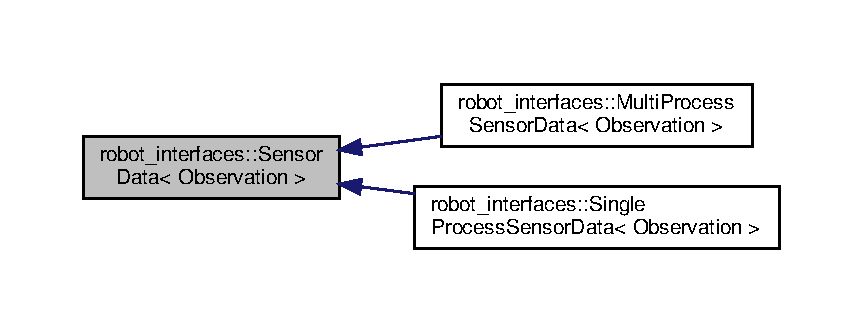
\includegraphics[width=350pt]{classrobot__interfaces_1_1SensorData__inherit__graph}
\end{center}
\end{figure}
\subsection*{Public Attributes}
\begin{DoxyCompactItemize}
\item 
\mbox{\Hypertarget{classrobot__interfaces_1_1SensorData_afb270cde8fa55814d76787589f05ce44}\label{classrobot__interfaces_1_1SensorData_afb270cde8fa55814d76787589f05ce44}} 
std\+::shared\+\_\+ptr$<$ time\+\_\+series\+::\+Time\+Series\+Interface$<$ Observation $>$ $>$ \hyperlink{classrobot__interfaces_1_1SensorData_afb270cde8fa55814d76787589f05ce44}{observation}
\begin{DoxyCompactList}\small\item\em Time series of the sensor observations. \end{DoxyCompactList}\end{DoxyCompactItemize}


\subsection{Detailed Description}
\subsubsection*{template$<$typename Observation$>$\newline
class robot\+\_\+interfaces\+::\+Sensor\+Data$<$ Observation $>$}

Contains the data coming from the sensors. 


\begin{DoxyTemplParams}{Template Parameters}
{\em Observation} & Type of the sensor observation. \\
\hline
\end{DoxyTemplParams}


The documentation for this class was generated from the following file\+:\begin{DoxyCompactItemize}
\item 
include/robot\+\_\+interfaces/sensors/\hyperlink{sensor__data_8hpp}{sensor\+\_\+data.\+hpp}\end{DoxyCompactItemize}

\hypertarget{classrobot__interfaces_1_1SensorDriver}{}\section{robot\+\_\+interfaces\+:\+:Sensor\+Driver$<$ Observation\+Type $>$ Class Template Reference}
\label{classrobot__interfaces_1_1SensorDriver}\index{robot\+\_\+interfaces\+::\+Sensor\+Driver$<$ Observation\+Type $>$@{robot\+\_\+interfaces\+::\+Sensor\+Driver$<$ Observation\+Type $>$}}


Base driver class from which all specific sensor drivers should derive.  




{\ttfamily \#include $<$sensor\+\_\+driver.\+hpp$>$}

\subsection*{Public Member Functions}
\begin{DoxyCompactItemize}
\item 
virtual Observation\+Type \hyperlink{classrobot__interfaces_1_1SensorDriver_a59a9918c43ba789dffb6e59f9790c6c2}{get\+\_\+observation} ()=0
\begin{DoxyCompactList}\small\item\em return the observation \end{DoxyCompactList}\end{DoxyCompactItemize}


\subsection{Detailed Description}
\subsubsection*{template$<$typename Observation\+Type$>$\newline
class robot\+\_\+interfaces\+::\+Sensor\+Driver$<$ Observation\+Type $>$}

Base driver class from which all specific sensor drivers should derive. 


\begin{DoxyTemplParams}{Template Parameters}
{\em Observation\+Type} & \\
\hline
\end{DoxyTemplParams}


\subsection{Member Function Documentation}
\mbox{\Hypertarget{classrobot__interfaces_1_1SensorDriver_a59a9918c43ba789dffb6e59f9790c6c2}\label{classrobot__interfaces_1_1SensorDriver_a59a9918c43ba789dffb6e59f9790c6c2}} 
\index{robot\+\_\+interfaces\+::\+Sensor\+Driver@{robot\+\_\+interfaces\+::\+Sensor\+Driver}!get\+\_\+observation@{get\+\_\+observation}}
\index{get\+\_\+observation@{get\+\_\+observation}!robot\+\_\+interfaces\+::\+Sensor\+Driver@{robot\+\_\+interfaces\+::\+Sensor\+Driver}}
\subsubsection{\texorpdfstring{get\+\_\+observation()}{get\_observation()}}
{\footnotesize\ttfamily template$<$typename Observation\+Type $>$ \\
virtual Observation\+Type \hyperlink{classrobot__interfaces_1_1SensorDriver}{robot\+\_\+interfaces\+::\+Sensor\+Driver}$<$ Observation\+Type $>$\+::get\+\_\+observation (\begin{DoxyParamCaption}{ }\end{DoxyParamCaption})\hspace{0.3cm}{\ttfamily [pure virtual]}}



return the observation 

\begin{DoxyReturn}{Returns}
depends on the observation structure of the sensor being interacted with 
\end{DoxyReturn}


The documentation for this class was generated from the following file\+:\begin{DoxyCompactItemize}
\item 
include/robot\+\_\+interfaces/sensors/\hyperlink{sensor__driver_8hpp}{sensor\+\_\+driver.\+hpp}\end{DoxyCompactItemize}

\hypertarget{classrobot__interfaces_1_1SensorFrontend}{}\section{robot\+\_\+interfaces\+:\+:Sensor\+Frontend$<$ Observation\+Type $>$ Class Template Reference}
\label{classrobot__interfaces_1_1SensorFrontend}\index{robot\+\_\+interfaces\+::\+Sensor\+Frontend$<$ Observation\+Type $>$@{robot\+\_\+interfaces\+::\+Sensor\+Frontend$<$ Observation\+Type $>$}}


Communication link between \hyperlink{classrobot__interfaces_1_1SensorData}{Sensor\+Data} and the user.  




{\ttfamily \#include $<$sensor\+\_\+frontend.\+hpp$>$}

\subsection*{Public Types}
\begin{DoxyCompactItemize}
\item 
\mbox{\Hypertarget{classrobot__interfaces_1_1SensorFrontend_a92f23f72c62ac7d32ca10742ddc5019f}\label{classrobot__interfaces_1_1SensorFrontend_a92f23f72c62ac7d32ca10742ddc5019f}} 
{\footnotesize template$<$typename Type $>$ }\\using {\bfseries Timeseries} = time\+\_\+series\+::\+Time\+Series$<$ Type $>$
\item 
\mbox{\Hypertarget{classrobot__interfaces_1_1SensorFrontend_a28f5b6f4a74b1fd3fcd45fde6df6f0f6}\label{classrobot__interfaces_1_1SensorFrontend_a28f5b6f4a74b1fd3fcd45fde6df6f0f6}} 
typedef time\+\_\+series\+::\+Timestamp {\bfseries Time\+Stamp}
\item 
\mbox{\Hypertarget{classrobot__interfaces_1_1SensorFrontend_a199456a7768dfeec4a5c4d2a59461b8d}\label{classrobot__interfaces_1_1SensorFrontend_a199456a7768dfeec4a5c4d2a59461b8d}} 
typedef time\+\_\+series\+::\+Index {\bfseries Time\+Index}
\end{DoxyCompactItemize}
\subsection*{Public Member Functions}
\begin{DoxyCompactItemize}
\item 
\mbox{\Hypertarget{classrobot__interfaces_1_1SensorFrontend_a87a137bd1903267ab407718ecc8375de}\label{classrobot__interfaces_1_1SensorFrontend_a87a137bd1903267ab407718ecc8375de}} 
{\bfseries Sensor\+Frontend} (std\+::shared\+\_\+ptr$<$ \hyperlink{classrobot__interfaces_1_1SensorData}{Sensor\+Data}$<$ Observation\+Type $>$$>$ sensor\+\_\+data)
\item 
\mbox{\Hypertarget{classrobot__interfaces_1_1SensorFrontend_a97eecb2518956b98b10484003aaccd48}\label{classrobot__interfaces_1_1SensorFrontend_a97eecb2518956b98b10484003aaccd48}} 
Observation\+Type {\bfseries get\+\_\+observation} (const Time\+Index t) const
\item 
\mbox{\Hypertarget{classrobot__interfaces_1_1SensorFrontend_a09051196a807afa040daff02d95bee52}\label{classrobot__interfaces_1_1SensorFrontend_a09051196a807afa040daff02d95bee52}} 
Observation\+Type {\bfseries get\+\_\+latest\+\_\+observation} () const
\item 
\mbox{\Hypertarget{classrobot__interfaces_1_1SensorFrontend_a0c6c91f9d6fc3c548e16fbc4657b80d4}\label{classrobot__interfaces_1_1SensorFrontend_a0c6c91f9d6fc3c548e16fbc4657b80d4}} 
Time\+Stamp {\bfseries get\+\_\+timestamp\+\_\+ms} (const Time\+Index t) const
\item 
\mbox{\Hypertarget{classrobot__interfaces_1_1SensorFrontend_ad7e09a895aa73549ca082e9db543dee1}\label{classrobot__interfaces_1_1SensorFrontend_ad7e09a895aa73549ca082e9db543dee1}} 
Time\+Index {\bfseries get\+\_\+current\+\_\+timeindex} () const
\end{DoxyCompactItemize}
\subsection*{Private Attributes}
\begin{DoxyCompactItemize}
\item 
\mbox{\Hypertarget{classrobot__interfaces_1_1SensorFrontend_a19b1505aed15c8e8e62c47e5de37d27f}\label{classrobot__interfaces_1_1SensorFrontend_a19b1505aed15c8e8e62c47e5de37d27f}} 
std\+::shared\+\_\+ptr$<$ \hyperlink{classrobot__interfaces_1_1SensorData}{Sensor\+Data}$<$ Observation\+Type $>$ $>$ {\bfseries sensor\+\_\+data\+\_\+}
\end{DoxyCompactItemize}


\subsection{Detailed Description}
\subsubsection*{template$<$typename Observation\+Type$>$\newline
class robot\+\_\+interfaces\+::\+Sensor\+Frontend$<$ Observation\+Type $>$}

Communication link between \hyperlink{classrobot__interfaces_1_1SensorData}{Sensor\+Data} and the user. 

Exposes the sensor data to the user to enable the user to get observations, timestamps, and timeindices from the timeseries.


\begin{DoxyTemplParams}{Template Parameters}
{\em Observation\+Type} & \\
\hline
\end{DoxyTemplParams}


The documentation for this class was generated from the following file\+:\begin{DoxyCompactItemize}
\item 
include/robot\+\_\+interfaces/sensors/\hyperlink{sensor__frontend_8hpp}{sensor\+\_\+frontend.\+hpp}\end{DoxyCompactItemize}

\hypertarget{classrobot__interfaces_1_1SensorLogger}{}\section{robot\+\_\+interfaces\+:\+:Sensor\+Logger$<$ Observation $>$ Class Template Reference}
\label{classrobot__interfaces_1_1SensorLogger}\index{robot\+\_\+interfaces\+::\+Sensor\+Logger$<$ Observation $>$@{robot\+\_\+interfaces\+::\+Sensor\+Logger$<$ Observation $>$}}


Record sensor observations and store them to a file.  




{\ttfamily \#include $<$sensor\+\_\+logger.\+hpp$>$}

\subsection*{Public Types}
\begin{DoxyCompactItemize}
\item 
\mbox{\Hypertarget{classrobot__interfaces_1_1SensorLogger_abfffa764f13c4b260416fbfe7e6a14ea}\label{classrobot__interfaces_1_1SensorLogger_abfffa764f13c4b260416fbfe7e6a14ea}} 
typedef std\+::shared\+\_\+ptr$<$ \hyperlink{classrobot__interfaces_1_1SensorData}{Sensor\+Data}$<$ Observation $>$ $>$ {\bfseries Data\+Ptr}
\end{DoxyCompactItemize}
\subsection*{Public Member Functions}
\begin{DoxyCompactItemize}
\item 
\hyperlink{classrobot__interfaces_1_1SensorLogger_aa2b7935cb32b53c49d6c3e541964d968}{Sensor\+Logger} (Data\+Ptr sensor\+\_\+data, size\+\_\+t buffer\+\_\+limit)
\begin{DoxyCompactList}\small\item\em Initialize the logger. \end{DoxyCompactList}\item 
\mbox{\Hypertarget{classrobot__interfaces_1_1SensorLogger_a1b2121061d96e3f026546f4359cfd769}\label{classrobot__interfaces_1_1SensorLogger_a1b2121061d96e3f026546f4359cfd769}} 
{\bfseries Sensor\+Logger} (\hyperlink{classrobot__interfaces_1_1SensorLogger}{Sensor\+Logger} \&\&)=default
\item 
void \hyperlink{classrobot__interfaces_1_1SensorLogger_a264f301075b8b4330b35776b3192bee9}{start} ()
\begin{DoxyCompactList}\small\item\em Start logging. \end{DoxyCompactList}\item 
void \hyperlink{classrobot__interfaces_1_1SensorLogger_ac4432aabd2e52401ec02bdcdfbc54e1f}{stop} ()
\begin{DoxyCompactList}\small\item\em Stop logging. \end{DoxyCompactList}\item 
\mbox{\Hypertarget{classrobot__interfaces_1_1SensorLogger_ab12a1bf654d7d09d3dd498d9d86476f2}\label{classrobot__interfaces_1_1SensorLogger_ab12a1bf654d7d09d3dd498d9d86476f2}} 
void \hyperlink{classrobot__interfaces_1_1SensorLogger_ab12a1bf654d7d09d3dd498d9d86476f2}{reset} ()
\begin{DoxyCompactList}\small\item\em Clear the log buffer. \end{DoxyCompactList}\item 
void \hyperlink{classrobot__interfaces_1_1SensorLogger_a1ab1fc25c3f20624a240430dff78b029}{stop\+\_\+and\+\_\+save} (const std\+::string \&filename)
\begin{DoxyCompactList}\small\item\em Stop logging and save logged messages to a file. \end{DoxyCompactList}\end{DoxyCompactItemize}
\subsection*{Private Member Functions}
\begin{DoxyCompactItemize}
\item 
\mbox{\Hypertarget{classrobot__interfaces_1_1SensorLogger_af05366bd0418ab2dea5a8f7de4031c5b}\label{classrobot__interfaces_1_1SensorLogger_af05366bd0418ab2dea5a8f7de4031c5b}} 
void \hyperlink{classrobot__interfaces_1_1SensorLogger_af05366bd0418ab2dea5a8f7de4031c5b}{loop} ()
\begin{DoxyCompactList}\small\item\em Get observations from sensor\+\_\+data\+\_\+ and add them to the buffer. \end{DoxyCompactList}\end{DoxyCompactItemize}
\subsection*{Private Attributes}
\begin{DoxyCompactItemize}
\item 
\mbox{\Hypertarget{classrobot__interfaces_1_1SensorLogger_a1771168bc44050029fac7f5943796ff9}\label{classrobot__interfaces_1_1SensorLogger_a1771168bc44050029fac7f5943796ff9}} 
Data\+Ptr {\bfseries sensor\+\_\+data\+\_\+}
\item 
\mbox{\Hypertarget{classrobot__interfaces_1_1SensorLogger_a0fcc2523aa7c8b05a17429c01ec19975}\label{classrobot__interfaces_1_1SensorLogger_a0fcc2523aa7c8b05a17429c01ec19975}} 
std\+::vector$<$ Observation $>$ {\bfseries buffer\+\_\+}
\item 
\mbox{\Hypertarget{classrobot__interfaces_1_1SensorLogger_a4ac7be763d55fa33344246fbe20598b6}\label{classrobot__interfaces_1_1SensorLogger_a4ac7be763d55fa33344246fbe20598b6}} 
size\+\_\+t {\bfseries buffer\+\_\+limit\+\_\+}
\item 
\mbox{\Hypertarget{classrobot__interfaces_1_1SensorLogger_a22eba71448f0428c1b4daf72243e3bf8}\label{classrobot__interfaces_1_1SensorLogger_a22eba71448f0428c1b4daf72243e3bf8}} 
std\+::thread {\bfseries buffer\+\_\+thread\+\_\+}
\item 
\mbox{\Hypertarget{classrobot__interfaces_1_1SensorLogger_a4af2d1815c0f205ea9c5c064723947f1}\label{classrobot__interfaces_1_1SensorLogger_a4af2d1815c0f205ea9c5c064723947f1}} 
bool {\bfseries enabled\+\_\+}
\end{DoxyCompactItemize}


\subsection{Detailed Description}
\subsubsection*{template$<$typename Observation$>$\newline
class robot\+\_\+interfaces\+::\+Sensor\+Logger$<$ Observation $>$}

Record sensor observations and store them to a file. 

Fetches observations from the given \hyperlink{classrobot__interfaces_1_1SensorData}{Sensor\+Data} and buffers them in memory. Buffered observations can be written to a file. For writing to file cereal is used, so the Observation type has to be serializable by cereal.

Usage Example\+:


\begin{DoxyCode}
\textcolor{keyword}{auto} logger = SensorLogger<int>(sensor\_data, BUFFER\_LIMIT);
logger.start();
\textcolor{comment}{// do something}
logger.stop\_and\_save(\textcolor{stringliteral}{"/tmp/sensordata.log"});
\end{DoxyCode}



\begin{DoxyTemplParams}{Template Parameters}
{\em Observation} & Typ of the observation that is recorded. \\
\hline
\end{DoxyTemplParams}


\subsection{Constructor \& Destructor Documentation}
\mbox{\Hypertarget{classrobot__interfaces_1_1SensorLogger_aa2b7935cb32b53c49d6c3e541964d968}\label{classrobot__interfaces_1_1SensorLogger_aa2b7935cb32b53c49d6c3e541964d968}} 
\index{robot\+\_\+interfaces\+::\+Sensor\+Logger@{robot\+\_\+interfaces\+::\+Sensor\+Logger}!Sensor\+Logger@{Sensor\+Logger}}
\index{Sensor\+Logger@{Sensor\+Logger}!robot\+\_\+interfaces\+::\+Sensor\+Logger@{robot\+\_\+interfaces\+::\+Sensor\+Logger}}
\subsubsection{\texorpdfstring{Sensor\+Logger()}{SensorLogger()}}
{\footnotesize\ttfamily template$<$typename Observation $>$ \\
\hyperlink{classrobot__interfaces_1_1SensorLogger}{robot\+\_\+interfaces\+::\+Sensor\+Logger}$<$ Observation $>$\+::\hyperlink{classrobot__interfaces_1_1SensorLogger}{Sensor\+Logger} (\begin{DoxyParamCaption}\item[{Data\+Ptr}]{sensor\+\_\+data,  }\item[{size\+\_\+t}]{buffer\+\_\+limit }\end{DoxyParamCaption})\hspace{0.3cm}{\ttfamily [inline]}}



Initialize the logger. 


\begin{DoxyParams}{Parameters}
{\em sensor\+\_\+data} & Pointer to the \hyperlink{classrobot__interfaces_1_1SensorData}{Sensor\+Data} instance from which observations are obtained. \\
\hline
{\em buffer\+\_\+limit} & Maximum number of observations that are logged. When this limit is reached, the logger will stop automatically, that is new observations are not logged anymore. \\
\hline
\end{DoxyParams}


\subsection{Member Function Documentation}
\mbox{\Hypertarget{classrobot__interfaces_1_1SensorLogger_a264f301075b8b4330b35776b3192bee9}\label{classrobot__interfaces_1_1SensorLogger_a264f301075b8b4330b35776b3192bee9}} 
\index{robot\+\_\+interfaces\+::\+Sensor\+Logger@{robot\+\_\+interfaces\+::\+Sensor\+Logger}!start@{start}}
\index{start@{start}!robot\+\_\+interfaces\+::\+Sensor\+Logger@{robot\+\_\+interfaces\+::\+Sensor\+Logger}}
\subsubsection{\texorpdfstring{start()}{start()}}
{\footnotesize\ttfamily template$<$typename Observation $>$ \\
void \hyperlink{classrobot__interfaces_1_1SensorLogger}{robot\+\_\+interfaces\+::\+Sensor\+Logger}$<$ Observation $>$\+::start (\begin{DoxyParamCaption}{ }\end{DoxyParamCaption})\hspace{0.3cm}{\ttfamily [inline]}}



Start logging. 

If the logger is already running, this is a noop. \mbox{\Hypertarget{classrobot__interfaces_1_1SensorLogger_ac4432aabd2e52401ec02bdcdfbc54e1f}\label{classrobot__interfaces_1_1SensorLogger_ac4432aabd2e52401ec02bdcdfbc54e1f}} 
\index{robot\+\_\+interfaces\+::\+Sensor\+Logger@{robot\+\_\+interfaces\+::\+Sensor\+Logger}!stop@{stop}}
\index{stop@{stop}!robot\+\_\+interfaces\+::\+Sensor\+Logger@{robot\+\_\+interfaces\+::\+Sensor\+Logger}}
\subsubsection{\texorpdfstring{stop()}{stop()}}
{\footnotesize\ttfamily template$<$typename Observation $>$ \\
void \hyperlink{classrobot__interfaces_1_1SensorLogger}{robot\+\_\+interfaces\+::\+Sensor\+Logger}$<$ Observation $>$\+::stop (\begin{DoxyParamCaption}{ }\end{DoxyParamCaption})\hspace{0.3cm}{\ttfamily [inline]}}



Stop logging. 

If the logger is already stopped, this is a noop. \mbox{\Hypertarget{classrobot__interfaces_1_1SensorLogger_a1ab1fc25c3f20624a240430dff78b029}\label{classrobot__interfaces_1_1SensorLogger_a1ab1fc25c3f20624a240430dff78b029}} 
\index{robot\+\_\+interfaces\+::\+Sensor\+Logger@{robot\+\_\+interfaces\+::\+Sensor\+Logger}!stop\+\_\+and\+\_\+save@{stop\+\_\+and\+\_\+save}}
\index{stop\+\_\+and\+\_\+save@{stop\+\_\+and\+\_\+save}!robot\+\_\+interfaces\+::\+Sensor\+Logger@{robot\+\_\+interfaces\+::\+Sensor\+Logger}}
\subsubsection{\texorpdfstring{stop\+\_\+and\+\_\+save()}{stop\_and\_save()}}
{\footnotesize\ttfamily template$<$typename Observation $>$ \\
void \hyperlink{classrobot__interfaces_1_1SensorLogger}{robot\+\_\+interfaces\+::\+Sensor\+Logger}$<$ Observation $>$\+::stop\+\_\+and\+\_\+save (\begin{DoxyParamCaption}\item[{const std\+::string \&}]{filename }\end{DoxyParamCaption})\hspace{0.3cm}{\ttfamily [inline]}}



Stop logging and save logged messages to a file. 


\begin{DoxyParams}{Parameters}
{\em filename} & Path to the output file. Existing files will be overwritten. \\
\hline
\end{DoxyParams}


The documentation for this class was generated from the following file\+:\begin{DoxyCompactItemize}
\item 
include/robot\+\_\+interfaces/sensors/sensor\+\_\+logger.\+hpp\end{DoxyCompactItemize}

\hypertarget{classrobot__interfaces_1_1SensorLogReader}{}\section{robot\+\_\+interfaces\+:\+:Sensor\+Log\+Reader$<$ Observation $>$ Class Template Reference}
\label{classrobot__interfaces_1_1SensorLogReader}\index{robot\+\_\+interfaces\+::\+Sensor\+Log\+Reader$<$ Observation $>$@{robot\+\_\+interfaces\+::\+Sensor\+Log\+Reader$<$ Observation $>$}}


Read the data from a sensor log file.  




{\ttfamily \#include $<$sensor\+\_\+log\+\_\+reader.\+hpp$>$}

\subsection*{Public Member Functions}
\begin{DoxyCompactItemize}
\item 
\hyperlink{classrobot__interfaces_1_1SensorLogReader_af98cfbebee2e96b24dcba44dff27b783}{Sensor\+Log\+Reader} (const std\+::string \&filename)
\begin{DoxyCompactList}\small\item\em Read data from the specified file. \end{DoxyCompactList}\item 
void \hyperlink{classrobot__interfaces_1_1SensorLogReader_a2632219304890e40ff770b1dfef72e6c}{read\+\_\+file} (const std\+::string \&filename)
\begin{DoxyCompactList}\small\item\em Read data from the specified file. \end{DoxyCompactList}\end{DoxyCompactItemize}
\subsection*{Public Attributes}
\begin{DoxyCompactItemize}
\item 
\mbox{\Hypertarget{classrobot__interfaces_1_1SensorLogReader_ae9bc7102e1de64979d2937f465eea9cc}\label{classrobot__interfaces_1_1SensorLogReader_ae9bc7102e1de64979d2937f465eea9cc}} 
std\+::vector$<$ Observation $>$ \hyperlink{classrobot__interfaces_1_1SensorLogReader_ae9bc7102e1de64979d2937f465eea9cc}{data}
\begin{DoxyCompactList}\small\item\em Data from the log file. \end{DoxyCompactList}\end{DoxyCompactItemize}


\subsection{Detailed Description}
\subsubsection*{template$<$typename Observation$>$\newline
class robot\+\_\+interfaces\+::\+Sensor\+Log\+Reader$<$ Observation $>$}

Read the data from a sensor log file. 

The data is read from the specified file and stored to the {\ttfamily data} member where it can be accessed.


\begin{DoxyTemplParams}{Template Parameters}
{\em Observation} & Type of the sensor observation. \\
\hline
\end{DoxyTemplParams}


\subsection{Constructor \& Destructor Documentation}
\mbox{\Hypertarget{classrobot__interfaces_1_1SensorLogReader_af98cfbebee2e96b24dcba44dff27b783}\label{classrobot__interfaces_1_1SensorLogReader_af98cfbebee2e96b24dcba44dff27b783}} 
\index{robot\+\_\+interfaces\+::\+Sensor\+Log\+Reader@{robot\+\_\+interfaces\+::\+Sensor\+Log\+Reader}!Sensor\+Log\+Reader@{Sensor\+Log\+Reader}}
\index{Sensor\+Log\+Reader@{Sensor\+Log\+Reader}!robot\+\_\+interfaces\+::\+Sensor\+Log\+Reader@{robot\+\_\+interfaces\+::\+Sensor\+Log\+Reader}}
\subsubsection{\texorpdfstring{Sensor\+Log\+Reader()}{SensorLogReader()}}
{\footnotesize\ttfamily template$<$typename Observation $>$ \\
\hyperlink{classrobot__interfaces_1_1SensorLogReader}{robot\+\_\+interfaces\+::\+Sensor\+Log\+Reader}$<$ Observation $>$\+::\hyperlink{classrobot__interfaces_1_1SensorLogReader}{Sensor\+Log\+Reader} (\begin{DoxyParamCaption}\item[{const std\+::string \&}]{filename }\end{DoxyParamCaption})\hspace{0.3cm}{\ttfamily [inline]}}



Read data from the specified file. 

The data is stored to \hyperlink{classrobot__interfaces_1_1SensorLogReader_ae9bc7102e1de64979d2937f465eea9cc}{Sensor\+Log\+Reader\+::data}.


\begin{DoxyParams}{Parameters}
{\em filename} & Path to the sensor log file. \\
\hline
\end{DoxyParams}


\subsection{Member Function Documentation}
\mbox{\Hypertarget{classrobot__interfaces_1_1SensorLogReader_a2632219304890e40ff770b1dfef72e6c}\label{classrobot__interfaces_1_1SensorLogReader_a2632219304890e40ff770b1dfef72e6c}} 
\index{robot\+\_\+interfaces\+::\+Sensor\+Log\+Reader@{robot\+\_\+interfaces\+::\+Sensor\+Log\+Reader}!read\+\_\+file@{read\+\_\+file}}
\index{read\+\_\+file@{read\+\_\+file}!robot\+\_\+interfaces\+::\+Sensor\+Log\+Reader@{robot\+\_\+interfaces\+::\+Sensor\+Log\+Reader}}
\subsubsection{\texorpdfstring{read\+\_\+file()}{read\_file()}}
{\footnotesize\ttfamily template$<$typename Observation $>$ \\
void \hyperlink{classrobot__interfaces_1_1SensorLogReader}{robot\+\_\+interfaces\+::\+Sensor\+Log\+Reader}$<$ Observation $>$\+::read\+\_\+file (\begin{DoxyParamCaption}\item[{const std\+::string \&}]{filename }\end{DoxyParamCaption})\hspace{0.3cm}{\ttfamily [inline]}}



Read data from the specified file. 

The data is stored to \hyperlink{classrobot__interfaces_1_1SensorLogReader_ae9bc7102e1de64979d2937f465eea9cc}{Sensor\+Log\+Reader\+::data}.


\begin{DoxyParams}{Parameters}
{\em filename} & Path to the sensor log file. \\
\hline
\end{DoxyParams}


The documentation for this class was generated from the following file\+:\begin{DoxyCompactItemize}
\item 
include/robot\+\_\+interfaces/sensors/\hyperlink{sensor__log__reader_8hpp}{sensor\+\_\+log\+\_\+reader.\+hpp}\end{DoxyCompactItemize}

\hypertarget{structrobot__interfaces_1_1SimpleNJointRobotTypes}{}\section{robot\+\_\+interfaces\+:\+:Simple\+N\+Joint\+Robot\+Types$<$ N $>$ Struct Template Reference}
\label{structrobot__interfaces_1_1SimpleNJointRobotTypes}\index{robot\+\_\+interfaces\+::\+Simple\+N\+Joint\+Robot\+Types$<$ N $>$@{robot\+\_\+interfaces\+::\+Simple\+N\+Joint\+Robot\+Types$<$ N $>$}}


Collection of types for a generic N-\/joint B\+L\+MC robot.  




{\ttfamily \#include $<$n\+\_\+joint\+\_\+robot\+\_\+types.\+hpp$>$}



Inheritance diagram for robot\+\_\+interfaces\+:\+:Simple\+N\+Joint\+Robot\+Types$<$ N $>$\+:
\nopagebreak
\begin{figure}[H]
\begin{center}
\leavevmode
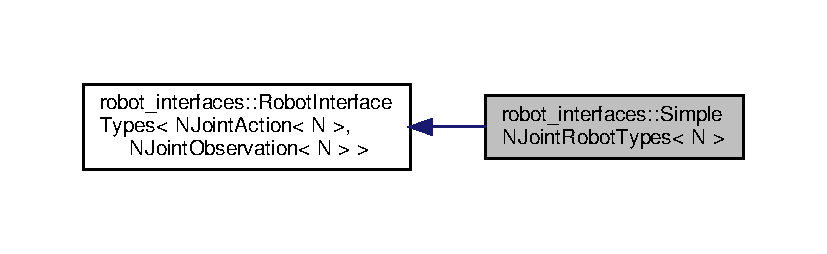
\includegraphics[width=350pt]{structrobot__interfaces_1_1SimpleNJointRobotTypes__inherit__graph}
\end{center}
\end{figure}


Collaboration diagram for robot\+\_\+interfaces\+:\+:Simple\+N\+Joint\+Robot\+Types$<$ N $>$\+:
\nopagebreak
\begin{figure}[H]
\begin{center}
\leavevmode
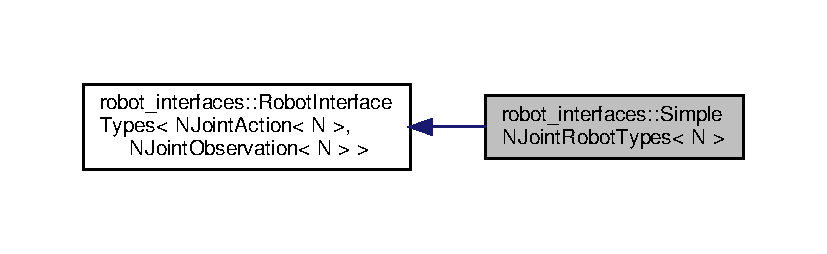
\includegraphics[width=350pt]{structrobot__interfaces_1_1SimpleNJointRobotTypes__coll__graph}
\end{center}
\end{figure}
\subsection*{Additional Inherited Members}


\subsection{Detailed Description}
\subsubsection*{template$<$size\+\_\+t N$>$\newline
struct robot\+\_\+interfaces\+::\+Simple\+N\+Joint\+Robot\+Types$<$ N $>$}

Collection of types for a generic N-\/joint B\+L\+MC robot. 

Defines all the types needed to set up an interface to a generic N-\/joint B\+L\+MC robot that expects as Action a simple vector of N torque commands and provides N observations containing measured joint angle, velocity and torque.


\begin{DoxyTemplParams}{Template Parameters}
{\em N} & Number of joints \\
\hline
\end{DoxyTemplParams}


The documentation for this struct was generated from the following file\+:\begin{DoxyCompactItemize}
\item 
include/robot\+\_\+interfaces/\hyperlink{n__joint__robot__types_8hpp}{n\+\_\+joint\+\_\+robot\+\_\+types.\+hpp}\end{DoxyCompactItemize}

\hypertarget{classrobot__interfaces_1_1SingleProcessRobotData}{}\section{robot\+\_\+interfaces\+:\+:Single\+Process\+Robot\+Data$<$ Action, Observation $>$ Class Template Reference}
\label{classrobot__interfaces_1_1SingleProcessRobotData}\index{robot\+\_\+interfaces\+::\+Single\+Process\+Robot\+Data$<$ Action, Observation $>$@{robot\+\_\+interfaces\+::\+Single\+Process\+Robot\+Data$<$ Action, Observation $>$}}


\hyperlink{classrobot__interfaces_1_1RobotData}{Robot\+Data} instance using single process time series.  




{\ttfamily \#include $<$robot\+\_\+data.\+hpp$>$}



Inheritance diagram for robot\+\_\+interfaces\+:\+:Single\+Process\+Robot\+Data$<$ Action, Observation $>$\+:
\nopagebreak
\begin{figure}[H]
\begin{center}
\leavevmode
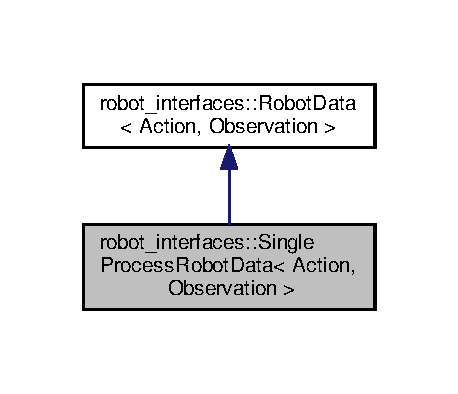
\includegraphics[width=220pt]{classrobot__interfaces_1_1SingleProcessRobotData__inherit__graph}
\end{center}
\end{figure}


Collaboration diagram for robot\+\_\+interfaces\+:\+:Single\+Process\+Robot\+Data$<$ Action, Observation $>$\+:
\nopagebreak
\begin{figure}[H]
\begin{center}
\leavevmode
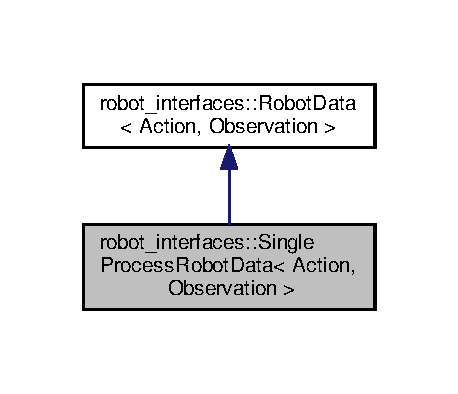
\includegraphics[width=220pt]{classrobot__interfaces_1_1SingleProcessRobotData__coll__graph}
\end{center}
\end{figure}
\subsection*{Public Member Functions}
\begin{DoxyCompactItemize}
\item 
\hyperlink{classrobot__interfaces_1_1SingleProcessRobotData_adcb9896c90464e27fb1cd2f303ca7cef}{Single\+Process\+Robot\+Data} (size\+\_\+t history\+\_\+length=1000)
\begin{DoxyCompactList}\small\item\em Construct the time series for the robot data. \end{DoxyCompactList}\end{DoxyCompactItemize}
\subsection*{Additional Inherited Members}


\subsection{Detailed Description}
\subsubsection*{template$<$typename Action, typename Observation$>$\newline
class robot\+\_\+interfaces\+::\+Single\+Process\+Robot\+Data$<$ Action, Observation $>$}

\hyperlink{classrobot__interfaces_1_1RobotData}{Robot\+Data} instance using single process time series. 

Use this class if all modules accessing the data are running in the same process. If modules run in separate processes, use \hyperlink{classrobot__interfaces_1_1MultiProcessRobotData}{Multi\+Process\+Robot\+Data} instead.

Contains all the input and output data of the robot. This means the
\begin{DoxyItemize}
\item {\ttfamily desired\+\_\+action} which was requested by the robot user
\item {\ttfamily applied\+\_\+action} which was actually applied and may not be and may not be identical to desired\+\_\+action for safety reasons
\item {\ttfamily observation} made by the robot
\item {\ttfamily status} which keeps track of timing issues and errors.
\end{DoxyItemize}

See this graph to understand how they relate to each other precisely in terms of time\+:

\begin{DoxyVerb}|------ t = 0 ------|------ t = 1 ------|
|----- action0 -----|----- action1 -----|
o                   o                   o
b                   b                   b
s                   s                   s
0                   1                   2
\end{DoxyVerb}



\begin{DoxyTemplParams}{Template Parameters}
{\em Action} & Type of the actions. \\
\hline
{\em Observation} & Type of the observations. \\
\hline
\end{DoxyTemplParams}
\begin{DoxySeeAlso}{See also}
\hyperlink{classrobot__interfaces_1_1MultiProcessRobotData}{Multi\+Process\+Robot\+Data} 
\end{DoxySeeAlso}
\begin{Desc}
\item[Examples\+: ]\par
\hyperlink{demo_8cpp-example}{demo.\+cpp}.\end{Desc}


\subsection{Constructor \& Destructor Documentation}
\mbox{\Hypertarget{classrobot__interfaces_1_1SingleProcessRobotData_adcb9896c90464e27fb1cd2f303ca7cef}\label{classrobot__interfaces_1_1SingleProcessRobotData_adcb9896c90464e27fb1cd2f303ca7cef}} 
\index{robot\+\_\+interfaces\+::\+Single\+Process\+Robot\+Data@{robot\+\_\+interfaces\+::\+Single\+Process\+Robot\+Data}!Single\+Process\+Robot\+Data@{Single\+Process\+Robot\+Data}}
\index{Single\+Process\+Robot\+Data@{Single\+Process\+Robot\+Data}!robot\+\_\+interfaces\+::\+Single\+Process\+Robot\+Data@{robot\+\_\+interfaces\+::\+Single\+Process\+Robot\+Data}}
\subsubsection{\texorpdfstring{Single\+Process\+Robot\+Data()}{SingleProcessRobotData()}}
{\footnotesize\ttfamily template$<$typename Action , typename Observation $>$ \\
\hyperlink{classrobot__interfaces_1_1SingleProcessRobotData}{robot\+\_\+interfaces\+::\+Single\+Process\+Robot\+Data}$<$ Action, Observation $>$\+::\hyperlink{classrobot__interfaces_1_1SingleProcessRobotData}{Single\+Process\+Robot\+Data} (\begin{DoxyParamCaption}\item[{size\+\_\+t}]{history\+\_\+length = {\ttfamily 1000} }\end{DoxyParamCaption})\hspace{0.3cm}{\ttfamily [inline]}}



Construct the time series for the robot data. 


\begin{DoxyParams}{Parameters}
{\em history\+\_\+length} & History length of the time series. \\
\hline
\end{DoxyParams}


The documentation for this class was generated from the following file\+:\begin{DoxyCompactItemize}
\item 
include/robot\+\_\+interfaces/\hyperlink{robot__data_8hpp}{robot\+\_\+data.\+hpp}\end{DoxyCompactItemize}

\hypertarget{classrobot__interfaces_1_1SingleProcessSensorData}{}\section{robot\+\_\+interfaces\+:\+:Single\+Process\+Sensor\+Data$<$ Observation $>$ Class Template Reference}
\label{classrobot__interfaces_1_1SingleProcessSensorData}\index{robot\+\_\+interfaces\+::\+Single\+Process\+Sensor\+Data$<$ Observation $>$@{robot\+\_\+interfaces\+::\+Single\+Process\+Sensor\+Data$<$ Observation $>$}}


\hyperlink{classrobot__interfaces_1_1SensorData}{Sensor\+Data} instance using single process time series.  




{\ttfamily \#include $<$sensor\+\_\+data.\+hpp$>$}



Inheritance diagram for robot\+\_\+interfaces\+:\+:Single\+Process\+Sensor\+Data$<$ Observation $>$\+:
\nopagebreak
\begin{figure}[H]
\begin{center}
\leavevmode
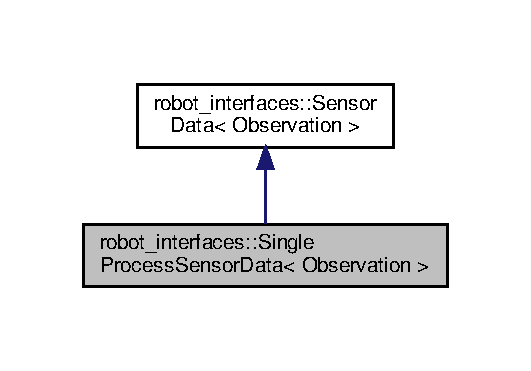
\includegraphics[width=255pt]{classrobot__interfaces_1_1SingleProcessSensorData__inherit__graph}
\end{center}
\end{figure}


Collaboration diagram for robot\+\_\+interfaces\+:\+:Single\+Process\+Sensor\+Data$<$ Observation $>$\+:
\nopagebreak
\begin{figure}[H]
\begin{center}
\leavevmode
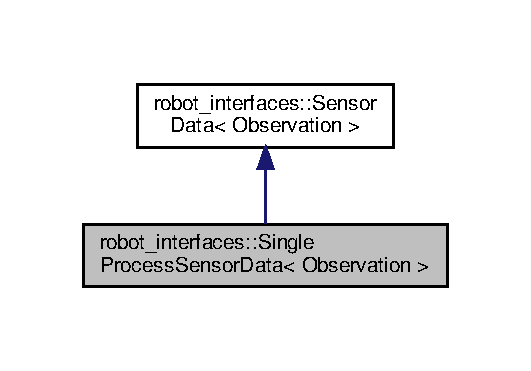
\includegraphics[width=255pt]{classrobot__interfaces_1_1SingleProcessSensorData__coll__graph}
\end{center}
\end{figure}
\subsection*{Public Member Functions}
\begin{DoxyCompactItemize}
\item 
\mbox{\Hypertarget{classrobot__interfaces_1_1SingleProcessSensorData_acebc7e34620a9adb3d80f82ea9da6836}\label{classrobot__interfaces_1_1SingleProcessSensorData_acebc7e34620a9adb3d80f82ea9da6836}} 
{\bfseries Single\+Process\+Sensor\+Data} (size\+\_\+t history\+\_\+length=1000)
\end{DoxyCompactItemize}
\subsection*{Additional Inherited Members}


\subsection{Detailed Description}
\subsubsection*{template$<$typename Observation$>$\newline
class robot\+\_\+interfaces\+::\+Single\+Process\+Sensor\+Data$<$ Observation $>$}

\hyperlink{classrobot__interfaces_1_1SensorData}{Sensor\+Data} instance using single process time series. 

Use this class if all modules accessing the data are running in the same process. If modules run in separate processes, use \hyperlink{classrobot__interfaces_1_1MultiProcessSensorData}{Multi\+Process\+Sensor\+Data} instead.

Contains the data coming from the sensors. 
\begin{DoxyTemplParams}{Template Parameters}
{\em Observation} & Type of the sensor observation. \\
\hline
\end{DoxyTemplParams}
\begin{DoxySeeAlso}{See also}
\hyperlink{classrobot__interfaces_1_1MultiProcessSensorData}{Multi\+Process\+Sensor\+Data} 
\end{DoxySeeAlso}


The documentation for this class was generated from the following file\+:\begin{DoxyCompactItemize}
\item 
include/robot\+\_\+interfaces/sensors/\hyperlink{sensor__data_8hpp}{sensor\+\_\+data.\+hpp}\end{DoxyCompactItemize}

\hypertarget{structrobot__interfaces_1_1Status}{}\section{robot\+\_\+interfaces\+:\+:Status Struct Reference}
\label{structrobot__interfaces_1_1Status}\index{robot\+\_\+interfaces\+::\+Status@{robot\+\_\+interfaces\+::\+Status}}


\hyperlink{structrobot__interfaces_1_1Status}{Status} information from the backend.  




{\ttfamily \#include $<$status.\+hpp$>$}



Inheritance diagram for robot\+\_\+interfaces\+:\+:Status\+:
\nopagebreak
\begin{figure}[H]
\begin{center}
\leavevmode
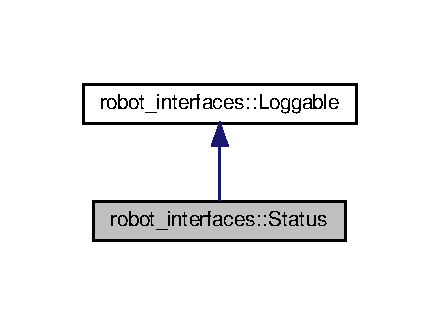
\includegraphics[width=211pt]{structrobot__interfaces_1_1Status__inherit__graph}
\end{center}
\end{figure}


Collaboration diagram for robot\+\_\+interfaces\+:\+:Status\+:
\nopagebreak
\begin{figure}[H]
\begin{center}
\leavevmode
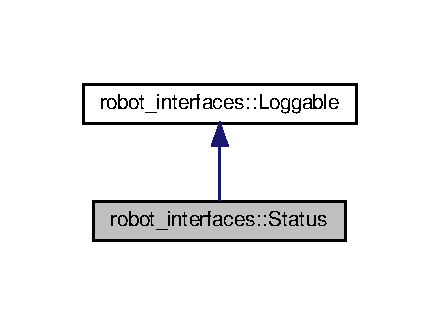
\includegraphics[width=211pt]{structrobot__interfaces_1_1Status__coll__graph}
\end{center}
\end{figure}
\subsection*{Public Types}
\begin{DoxyCompactItemize}
\item 
enum \hyperlink{structrobot__interfaces_1_1Status_a88f1cb8387648815ca75754985bdb3b6}{Error\+Status} \{ \hyperlink{structrobot__interfaces_1_1Status_a88f1cb8387648815ca75754985bdb3b6ad306b6fdee05fe87455110ddf6501e6c}{Error\+Status\+::\+N\+O\+\_\+\+E\+R\+R\+OR} = 0, 
\hyperlink{structrobot__interfaces_1_1Status_a88f1cb8387648815ca75754985bdb3b6a5cd5516428d081129a4aea1db455272e}{Error\+Status\+::\+D\+R\+I\+V\+E\+R\+\_\+\+E\+R\+R\+OR}, 
\hyperlink{structrobot__interfaces_1_1Status_a88f1cb8387648815ca75754985bdb3b6ac44598cc3395b73e9fd2866f42945bd3}{Error\+Status\+::\+B\+A\+C\+K\+E\+N\+D\+\_\+\+E\+R\+R\+OR}
 \}\begin{DoxyCompactList}\small\item\em Different types of errors that can occur in the backend. \end{DoxyCompactList}
\end{DoxyCompactItemize}
\subsection*{Public Member Functions}
\begin{DoxyCompactItemize}
\item 
void \hyperlink{structrobot__interfaces_1_1Status_aa5bbec49d6faba7507abc8772dec505d}{set\+\_\+error} (\hyperlink{structrobot__interfaces_1_1Status_a88f1cb8387648815ca75754985bdb3b6}{Error\+Status} error\+\_\+type, const std\+::string \&message)
\begin{DoxyCompactList}\small\item\em Set error. \end{DoxyCompactList}\item 
bool \hyperlink{structrobot__interfaces_1_1Status_a83507b0921dc1e67e690b34daa3bcbc3}{has\+\_\+error} () const
\begin{DoxyCompactList}\small\item\em Check if an error is set. \end{DoxyCompactList}\item 
\mbox{\Hypertarget{structrobot__interfaces_1_1Status_a5531f83e2ef30f7629548194b4e3e9da}\label{structrobot__interfaces_1_1Status_a5531f83e2ef30f7629548194b4e3e9da}} 
{\footnotesize template$<$class Archive $>$ }\\void {\bfseries serialize} (Archive \&archive)
\item 
\mbox{\Hypertarget{structrobot__interfaces_1_1Status_a2cd6543deb86d878ba43153c18d2fadb}\label{structrobot__interfaces_1_1Status_a2cd6543deb86d878ba43153c18d2fadb}} 
std\+::vector$<$ std\+::string $>$ {\bfseries get\+\_\+name} () override
\item 
\mbox{\Hypertarget{structrobot__interfaces_1_1Status_af530134f33fa21c02d1157636c385fa3}\label{structrobot__interfaces_1_1Status_af530134f33fa21c02d1157636c385fa3}} 
std\+::vector$<$ std\+::vector$<$ double $>$ $>$ {\bfseries get\+\_\+data} () override
\end{DoxyCompactItemize}
\subsection*{Public Attributes}
\begin{DoxyCompactItemize}
\item 
uint32\+\_\+t \hyperlink{structrobot__interfaces_1_1Status_a8ccb682cd2ba81059991f3b0b9ff0c00}{action\+\_\+repetitions} = 0
\begin{DoxyCompactList}\small\item\em Number of times the current action has been repeated. \end{DoxyCompactList}\item 
\hyperlink{structrobot__interfaces_1_1Status_a88f1cb8387648815ca75754985bdb3b6}{Error\+Status} \hyperlink{structrobot__interfaces_1_1Status_a80ffe66121d425d48386b39984cd4c7b}{error\+\_\+status} = \hyperlink{structrobot__interfaces_1_1Status_a88f1cb8387648815ca75754985bdb3b6ad306b6fdee05fe87455110ddf6501e6c}{Error\+Status\+::\+N\+O\+\_\+\+E\+R\+R\+OR}
\begin{DoxyCompactList}\small\item\em Indicates if there is an error and, if yes, in which component. \end{DoxyCompactList}\item 
std\+::string \hyperlink{structrobot__interfaces_1_1Status_a7da10fb73cd19f2840c438d321eac744}{error\+\_\+message}
\begin{DoxyCompactList}\small\item\em Human-\/readable message describing the error. \end{DoxyCompactList}\end{DoxyCompactItemize}


\subsection{Detailed Description}
\hyperlink{structrobot__interfaces_1_1Status}{Status} information from the backend. 

Used to report status information that is not directly robot-\/related from the backend to the frontend. 

\subsection{Member Enumeration Documentation}
\mbox{\Hypertarget{structrobot__interfaces_1_1Status_a88f1cb8387648815ca75754985bdb3b6}\label{structrobot__interfaces_1_1Status_a88f1cb8387648815ca75754985bdb3b6}} 
\index{robot\+\_\+interfaces\+::\+Status@{robot\+\_\+interfaces\+::\+Status}!Error\+Status@{Error\+Status}}
\index{Error\+Status@{Error\+Status}!robot\+\_\+interfaces\+::\+Status@{robot\+\_\+interfaces\+::\+Status}}
\subsubsection{\texorpdfstring{Error\+Status}{ErrorStatus}}
{\footnotesize\ttfamily enum \hyperlink{structrobot__interfaces_1_1Status_a88f1cb8387648815ca75754985bdb3b6}{robot\+\_\+interfaces\+::\+Status\+::\+Error\+Status}\hspace{0.3cm}{\ttfamily [strong]}}



Different types of errors that can occur in the backend. 

\begin{DoxyEnumFields}{Enumerator}
\raisebox{\heightof{T}}[0pt][0pt]{\index{N\+O\+\_\+\+E\+R\+R\+OR@{N\+O\+\_\+\+E\+R\+R\+OR}!robot\+\_\+interfaces\+::\+Status@{robot\+\_\+interfaces\+::\+Status}}\index{robot\+\_\+interfaces\+::\+Status@{robot\+\_\+interfaces\+::\+Status}!N\+O\+\_\+\+E\+R\+R\+OR@{N\+O\+\_\+\+E\+R\+R\+OR}}}\mbox{\Hypertarget{structrobot__interfaces_1_1Status_a88f1cb8387648815ca75754985bdb3b6ad306b6fdee05fe87455110ddf6501e6c}\label{structrobot__interfaces_1_1Status_a88f1cb8387648815ca75754985bdb3b6ad306b6fdee05fe87455110ddf6501e6c}} 
N\+O\+\_\+\+E\+R\+R\+OR&Indicates that there is no error. \\
\hline

\raisebox{\heightof{T}}[0pt][0pt]{\index{D\+R\+I\+V\+E\+R\+\_\+\+E\+R\+R\+OR@{D\+R\+I\+V\+E\+R\+\_\+\+E\+R\+R\+OR}!robot\+\_\+interfaces\+::\+Status@{robot\+\_\+interfaces\+::\+Status}}\index{robot\+\_\+interfaces\+::\+Status@{robot\+\_\+interfaces\+::\+Status}!D\+R\+I\+V\+E\+R\+\_\+\+E\+R\+R\+OR@{D\+R\+I\+V\+E\+R\+\_\+\+E\+R\+R\+OR}}}\mbox{\Hypertarget{structrobot__interfaces_1_1Status_a88f1cb8387648815ca75754985bdb3b6a5cd5516428d081129a4aea1db455272e}\label{structrobot__interfaces_1_1Status_a88f1cb8387648815ca75754985bdb3b6a5cd5516428d081129a4aea1db455272e}} 
D\+R\+I\+V\+E\+R\+\_\+\+E\+R\+R\+OR&Error reported from the \hyperlink{classrobot__interfaces_1_1RobotDriver}{Robot\+Driver}. An error reported by the low level robot driver (see \hyperlink{classrobot__interfaces_1_1RobotDriver}{Robot\+Driver}). This is depending on the driver implementation. It can, for example, be used to report some hardware failure). \\
\hline

\raisebox{\heightof{T}}[0pt][0pt]{\index{B\+A\+C\+K\+E\+N\+D\+\_\+\+E\+R\+R\+OR@{B\+A\+C\+K\+E\+N\+D\+\_\+\+E\+R\+R\+OR}!robot\+\_\+interfaces\+::\+Status@{robot\+\_\+interfaces\+::\+Status}}\index{robot\+\_\+interfaces\+::\+Status@{robot\+\_\+interfaces\+::\+Status}!B\+A\+C\+K\+E\+N\+D\+\_\+\+E\+R\+R\+OR@{B\+A\+C\+K\+E\+N\+D\+\_\+\+E\+R\+R\+OR}}}\mbox{\Hypertarget{structrobot__interfaces_1_1Status_a88f1cb8387648815ca75754985bdb3b6ac44598cc3395b73e9fd2866f42945bd3}\label{structrobot__interfaces_1_1Status_a88f1cb8387648815ca75754985bdb3b6ac44598cc3395b73e9fd2866f42945bd3}} 
B\+A\+C\+K\+E\+N\+D\+\_\+\+E\+R\+R\+OR&Error from the \hyperlink{classrobot__interfaces_1_1RobotBackend}{Robot\+Backend}. An error which is issued by the back end itself, for example if no new action is provided and the allowed number of repetitions is exceeded. \\
\hline

\end{DoxyEnumFields}


\subsection{Member Function Documentation}
\mbox{\Hypertarget{structrobot__interfaces_1_1Status_a83507b0921dc1e67e690b34daa3bcbc3}\label{structrobot__interfaces_1_1Status_a83507b0921dc1e67e690b34daa3bcbc3}} 
\index{robot\+\_\+interfaces\+::\+Status@{robot\+\_\+interfaces\+::\+Status}!has\+\_\+error@{has\+\_\+error}}
\index{has\+\_\+error@{has\+\_\+error}!robot\+\_\+interfaces\+::\+Status@{robot\+\_\+interfaces\+::\+Status}}
\subsubsection{\texorpdfstring{has\+\_\+error()}{has\_error()}}
{\footnotesize\ttfamily bool robot\+\_\+interfaces\+::\+Status\+::has\+\_\+error (\begin{DoxyParamCaption}{ }\end{DoxyParamCaption}) const\hspace{0.3cm}{\ttfamily [inline]}}



Check if an error is set. 

\begin{DoxyNote}{Note}
If there is an error reported in the status, the robot is not in an operational state anymore. Trying to append another action in the \hyperlink{classrobot__interfaces_1_1RobotFrontend}{Robot\+Frontend} will result in an exception in this case.
\end{DoxyNote}
See \hyperlink{structrobot__interfaces_1_1Status_a80ffe66121d425d48386b39984cd4c7b}{error\+\_\+status} and \hyperlink{structrobot__interfaces_1_1Status_a7da10fb73cd19f2840c438d321eac744}{error\+\_\+message} for more details on the error. \mbox{\Hypertarget{structrobot__interfaces_1_1Status_aa5bbec49d6faba7507abc8772dec505d}\label{structrobot__interfaces_1_1Status_aa5bbec49d6faba7507abc8772dec505d}} 
\index{robot\+\_\+interfaces\+::\+Status@{robot\+\_\+interfaces\+::\+Status}!set\+\_\+error@{set\+\_\+error}}
\index{set\+\_\+error@{set\+\_\+error}!robot\+\_\+interfaces\+::\+Status@{robot\+\_\+interfaces\+::\+Status}}
\subsubsection{\texorpdfstring{set\+\_\+error()}{set\_error()}}
{\footnotesize\ttfamily void robot\+\_\+interfaces\+::\+Status\+::set\+\_\+error (\begin{DoxyParamCaption}\item[{\hyperlink{structrobot__interfaces_1_1Status_a88f1cb8387648815ca75754985bdb3b6}{Error\+Status}}]{error\+\_\+type,  }\item[{const std\+::string \&}]{message }\end{DoxyParamCaption})\hspace{0.3cm}{\ttfamily [inline]}}



Set error. 

If another error was set before, the old one is kept and the new one ignored.


\begin{DoxyParams}{Parameters}
{\em error\+\_\+type} & The type of the error. \\
\hline
{\em message} & Error message. \\
\hline
\end{DoxyParams}


\subsection{Member Data Documentation}
\mbox{\Hypertarget{structrobot__interfaces_1_1Status_a8ccb682cd2ba81059991f3b0b9ff0c00}\label{structrobot__interfaces_1_1Status_a8ccb682cd2ba81059991f3b0b9ff0c00}} 
\index{robot\+\_\+interfaces\+::\+Status@{robot\+\_\+interfaces\+::\+Status}!action\+\_\+repetitions@{action\+\_\+repetitions}}
\index{action\+\_\+repetitions@{action\+\_\+repetitions}!robot\+\_\+interfaces\+::\+Status@{robot\+\_\+interfaces\+::\+Status}}
\subsubsection{\texorpdfstring{action\+\_\+repetitions}{action\_repetitions}}
{\footnotesize\ttfamily uint32\+\_\+t robot\+\_\+interfaces\+::\+Status\+::action\+\_\+repetitions = 0}



Number of times the current action has been repeated. 

If the back end wants to apply the next action but no new action was provided by the user in time, it may (depending on configuration) repeat the previous action. Each time this happens, {\ttfamily action\+\_\+repetitions} is increased by one. Once a new action is provided, it will be reset to zero.

See also \hyperlink{md_docs_timeseries_next-action-not-in-time}{When Next Action Is Not Provided In Time}. \mbox{\Hypertarget{structrobot__interfaces_1_1Status_a7da10fb73cd19f2840c438d321eac744}\label{structrobot__interfaces_1_1Status_a7da10fb73cd19f2840c438d321eac744}} 
\index{robot\+\_\+interfaces\+::\+Status@{robot\+\_\+interfaces\+::\+Status}!error\+\_\+message@{error\+\_\+message}}
\index{error\+\_\+message@{error\+\_\+message}!robot\+\_\+interfaces\+::\+Status@{robot\+\_\+interfaces\+::\+Status}}
\subsubsection{\texorpdfstring{error\+\_\+message}{error\_message}}
{\footnotesize\ttfamily std\+::string robot\+\_\+interfaces\+::\+Status\+::error\+\_\+message}



Human-\/readable message describing the error. 

Value is undefined if {\ttfamily error\+\_\+status == N\+O\+\_\+\+E\+R\+R\+OR}. \mbox{\Hypertarget{structrobot__interfaces_1_1Status_a80ffe66121d425d48386b39984cd4c7b}\label{structrobot__interfaces_1_1Status_a80ffe66121d425d48386b39984cd4c7b}} 
\index{robot\+\_\+interfaces\+::\+Status@{robot\+\_\+interfaces\+::\+Status}!error\+\_\+status@{error\+\_\+status}}
\index{error\+\_\+status@{error\+\_\+status}!robot\+\_\+interfaces\+::\+Status@{robot\+\_\+interfaces\+::\+Status}}
\subsubsection{\texorpdfstring{error\+\_\+status}{error\_status}}
{\footnotesize\ttfamily \hyperlink{structrobot__interfaces_1_1Status_a88f1cb8387648815ca75754985bdb3b6}{Error\+Status} robot\+\_\+interfaces\+::\+Status\+::error\+\_\+status = \hyperlink{structrobot__interfaces_1_1Status_a88f1cb8387648815ca75754985bdb3b6ad306b6fdee05fe87455110ddf6501e6c}{Error\+Status\+::\+N\+O\+\_\+\+E\+R\+R\+OR}}



Indicates if there is an error and, if yes, in which component. 

\begin{DoxyNote}{Note}
If there is an error reported in the status, the robot is not in an operational state anymore. Trying to append another action in the \hyperlink{classrobot__interfaces_1_1RobotFrontend}{Robot\+Frontend} will result in an exception in this case.
\end{DoxyNote}
\begin{DoxySeeAlso}{See also}
\hyperlink{structrobot__interfaces_1_1Status_a7da10fb73cd19f2840c438d321eac744}{error\+\_\+message} for more information on the error. 

\hyperlink{structrobot__interfaces_1_1Status_a83507b0921dc1e67e690b34daa3bcbc3}{has\+\_\+error()} 
\end{DoxySeeAlso}


The documentation for this struct was generated from the following file\+:\begin{DoxyCompactItemize}
\item 
include/robot\+\_\+interfaces/\hyperlink{status_8hpp}{status.\+hpp}\end{DoxyCompactItemize}

\chapter{File Documentation}
\hypertarget{demo_8cpp}{}\section{demos/demo.cpp File Reference}
\label{demo_8cpp}\index{demos/demo.\+cpp@{demos/demo.\+cpp}}


Minimal demo of robot driver, backend and frontend.  


{\ttfamily \#include \char`\"{}robot\+\_\+interfaces/example.\+hpp\char`\"{}}\newline
{\ttfamily \#include \char`\"{}robot\+\_\+interfaces/monitored\+\_\+robot\+\_\+driver.\+hpp\char`\"{}}\newline
{\ttfamily \#include \char`\"{}robot\+\_\+interfaces/robot.\+hpp\char`\"{}}\newline
{\ttfamily \#include \char`\"{}robot\+\_\+interfaces/robot\+\_\+backend.\+hpp\char`\"{}}\newline
{\ttfamily \#include \char`\"{}robot\+\_\+interfaces/robot\+\_\+driver.\+hpp\char`\"{}}\newline
{\ttfamily \#include \char`\"{}robot\+\_\+interfaces/robot\+\_\+frontend.\+hpp\char`\"{}}\newline
{\ttfamily \#include \char`\"{}robot\+\_\+interfaces/status.\+hpp\char`\"{}}\newline
{\ttfamily \#include $<$memory$>$}\newline
Include dependency graph for demo.\+cpp\+:
\nopagebreak
\begin{figure}[H]
\begin{center}
\leavevmode
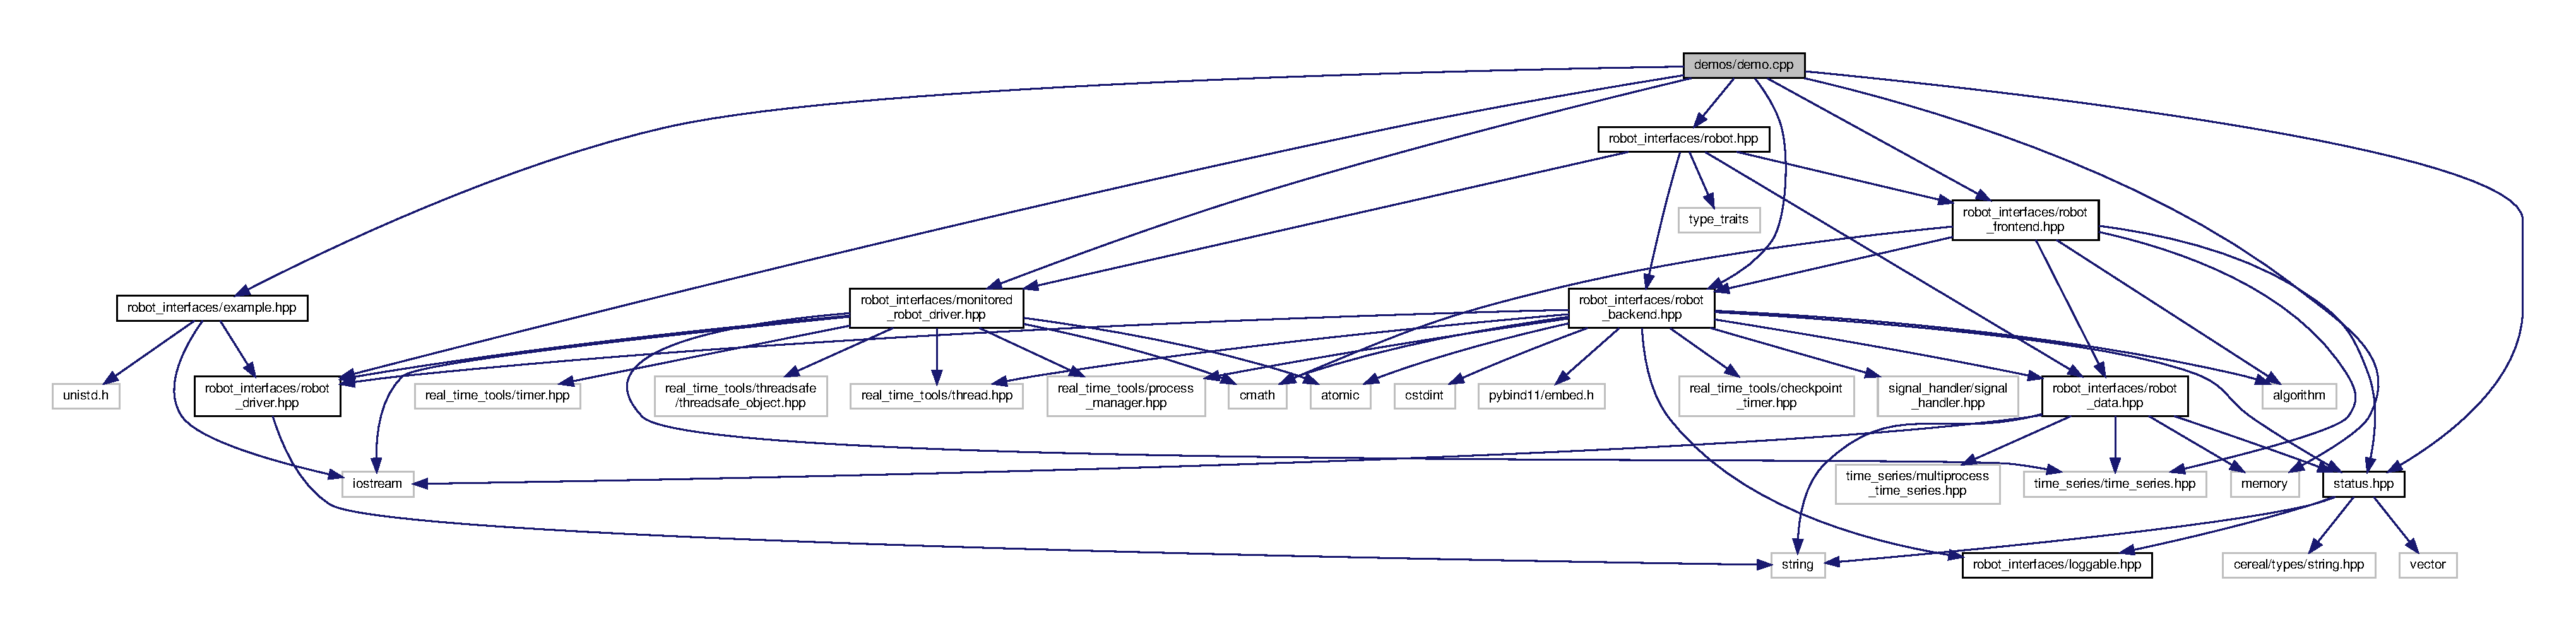
\includegraphics[width=350pt]{demo_8cpp__incl}
\end{center}
\end{figure}
\subsection*{Functions}
\begin{DoxyCompactItemize}
\item 
\mbox{\Hypertarget{demo_8cpp_ae66f6b31b5ad750f1fe042a706a4e3d4}\label{demo_8cpp_ae66f6b31b5ad750f1fe042a706a4e3d4}} 
int {\bfseries main} ()
\end{DoxyCompactItemize}


\subsection{Detailed Description}
Minimal demo of robot driver, backend and frontend. 

\begin{DoxyAuthor}{Author}
Vincent Berenz license License B\+S\+D-\/3-\/\+Clause 
\end{DoxyAuthor}
\begin{DoxyCopyright}{Copyright}
Copyright (c) 2019, Max Planck Gesellschaft. 
\end{DoxyCopyright}

\hypertarget{demo__multiprocess__backend_8cpp}{}\section{demos/demo\+\_\+multiprocess\+\_\+backend.cpp File Reference}
\label{demo__multiprocess__backend_8cpp}\index{demos/demo\+\_\+multiprocess\+\_\+backend.\+cpp@{demos/demo\+\_\+multiprocess\+\_\+backend.\+cpp}}


Minimal demo of robot driver/backend running in its own process.  


{\ttfamily \#include $<$memory$>$}\newline
{\ttfamily \#include \char`\"{}robot\+\_\+interfaces/robot\+\_\+backend.\+hpp\char`\"{}}\newline
{\ttfamily \#include \char`\"{}robot\+\_\+interfaces/robot\+\_\+driver.\+hpp\char`\"{}}\newline
{\ttfamily \#include \char`\"{}types.\+hpp\char`\"{}}\newline
Include dependency graph for demo\+\_\+multiprocess\+\_\+backend.\+cpp\+:
\nopagebreak
\begin{figure}[H]
\begin{center}
\leavevmode
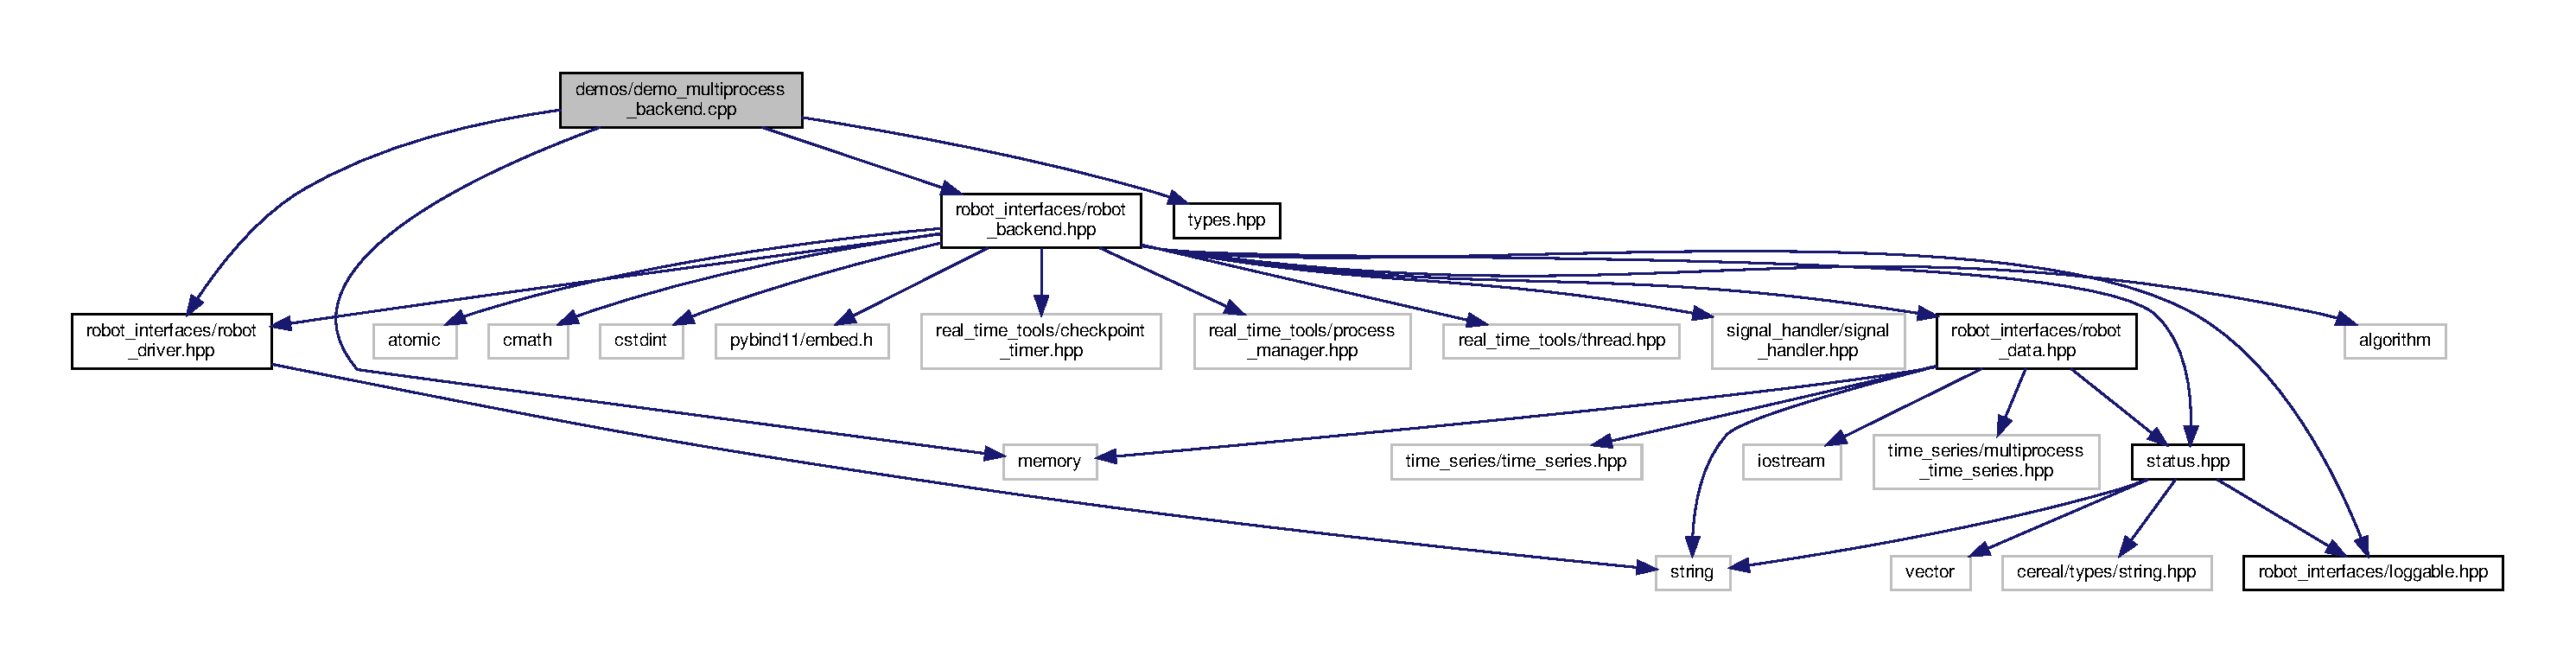
\includegraphics[width=350pt]{demo__multiprocess__backend_8cpp__incl}
\end{center}
\end{figure}
\subsection*{Classes}
\begin{DoxyCompactItemize}
\item 
class \hyperlink{classDriver}{Driver}
\end{DoxyCompactItemize}
\subsection*{Functions}
\begin{DoxyCompactItemize}
\item 
\mbox{\Hypertarget{demo__multiprocess__backend_8cpp_ae66f6b31b5ad750f1fe042a706a4e3d4}\label{demo__multiprocess__backend_8cpp_ae66f6b31b5ad750f1fe042a706a4e3d4}} 
int {\bfseries main} ()
\end{DoxyCompactItemize}


\subsection{Detailed Description}
Minimal demo of robot driver/backend running in its own process. 

\begin{DoxyAuthor}{Author}
Vincent Berenz, Felix Widmaier license License B\+S\+D-\/3-\/\+Clause 
\end{DoxyAuthor}
\begin{DoxyCopyright}{Copyright}
Copyright (c) 2019-\/2020, Max Planck Gesellschaft. 
\end{DoxyCopyright}

\hypertarget{demo__multiprocess__frontend_8cpp}{}\section{demos/demo\+\_\+multiprocess\+\_\+frontend.cpp File Reference}
\label{demo__multiprocess__frontend_8cpp}\index{demos/demo\+\_\+multiprocess\+\_\+frontend.\+cpp@{demos/demo\+\_\+multiprocess\+\_\+frontend.\+cpp}}


Minimal demo of robot frontend running in its own process.  


{\ttfamily \#include $<$memory$>$}\newline
{\ttfamily \#include \char`\"{}robot\+\_\+interfaces/robot\+\_\+frontend.\+hpp\char`\"{}}\newline
{\ttfamily \#include \char`\"{}types.\+hpp\char`\"{}}\newline
Include dependency graph for demo\+\_\+multiprocess\+\_\+frontend.\+cpp\+:
\nopagebreak
\begin{figure}[H]
\begin{center}
\leavevmode
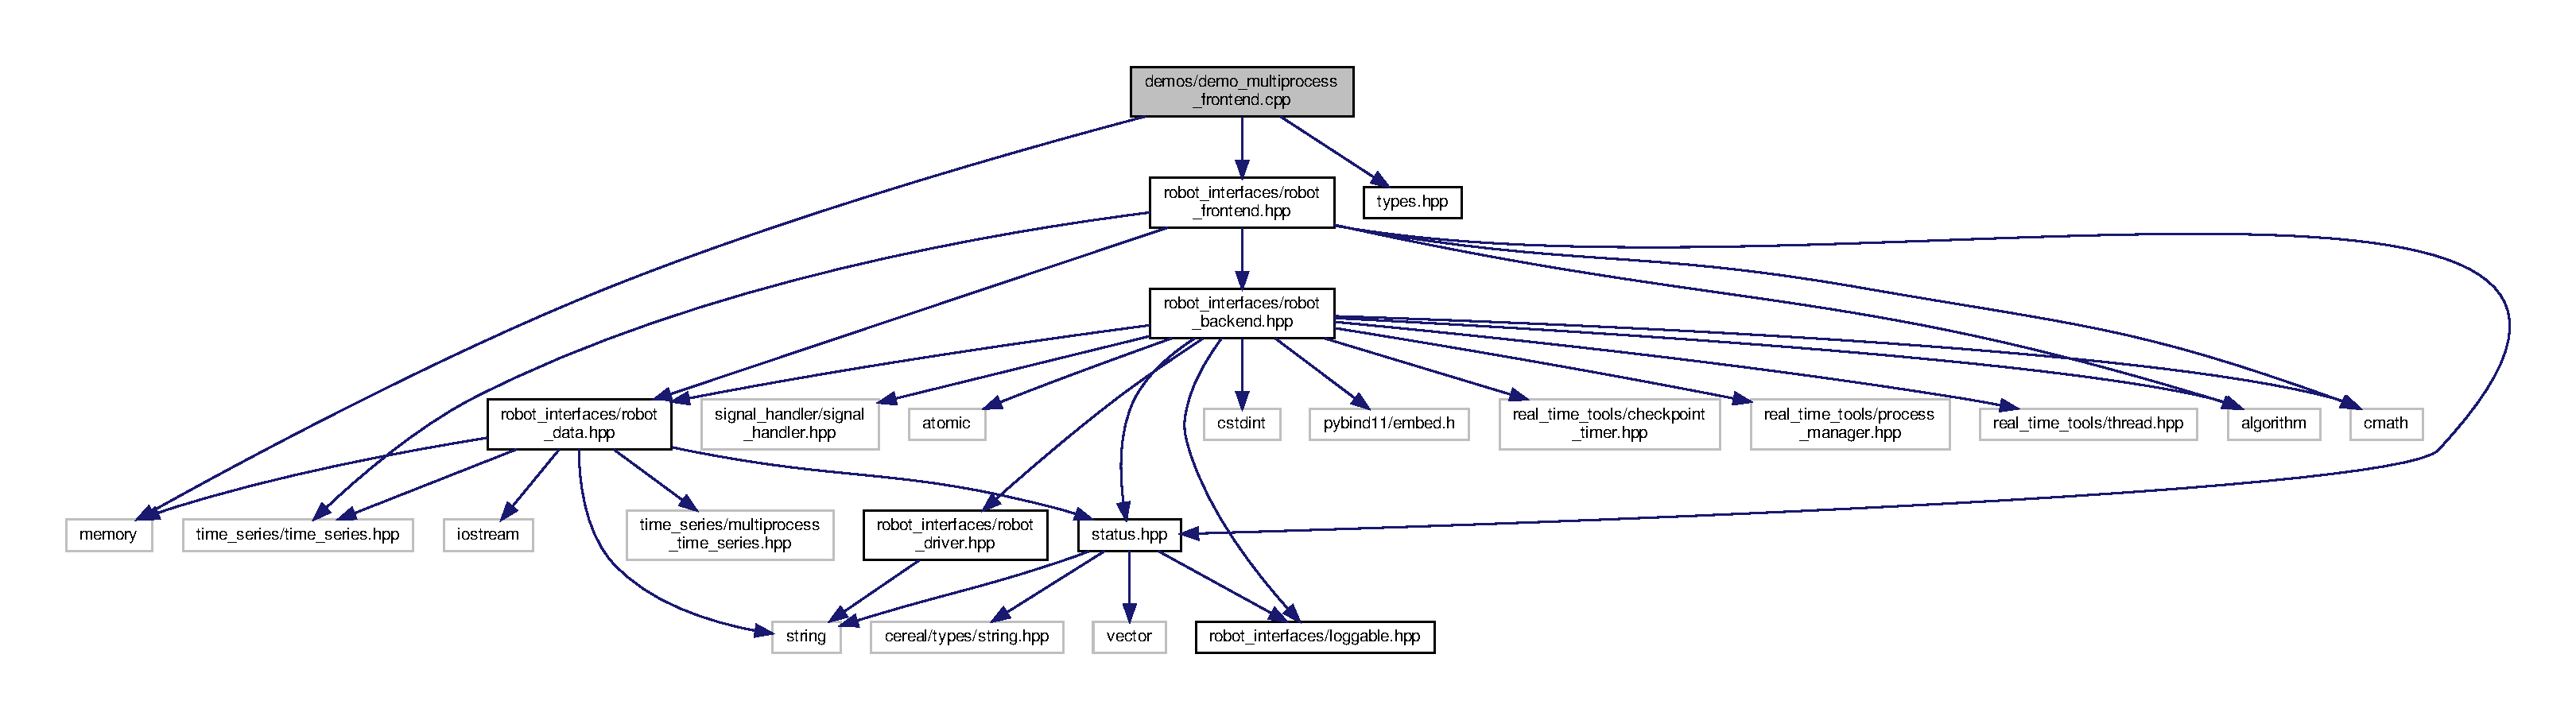
\includegraphics[width=350pt]{demo__multiprocess__frontend_8cpp__incl}
\end{center}
\end{figure}
\subsection*{Functions}
\begin{DoxyCompactItemize}
\item 
\mbox{\Hypertarget{demo__multiprocess__frontend_8cpp_ae66f6b31b5ad750f1fe042a706a4e3d4}\label{demo__multiprocess__frontend_8cpp_ae66f6b31b5ad750f1fe042a706a4e3d4}} 
int {\bfseries main} ()
\end{DoxyCompactItemize}


\subsection{Detailed Description}
Minimal demo of robot frontend running in its own process. 

\begin{DoxyAuthor}{Author}
Vincent Berenz, Felix Widmaier license License B\+S\+D-\/3-\/\+Clause 
\end{DoxyAuthor}
\begin{DoxyCopyright}{Copyright}
Copyright (c) 2019-\/2020, Max Planck Gesellschaft. 
\end{DoxyCopyright}

\hypertarget{demos_2types_8hpp}{}\section{demos/types.hpp File Reference}
\label{demos_2types_8hpp}\index{demos/types.\+hpp@{demos/types.\+hpp}}


license License B\+S\+D-\/3-\/\+Clause  


This graph shows which files directly or indirectly include this file\+:
\nopagebreak
\begin{figure}[H]
\begin{center}
\leavevmode
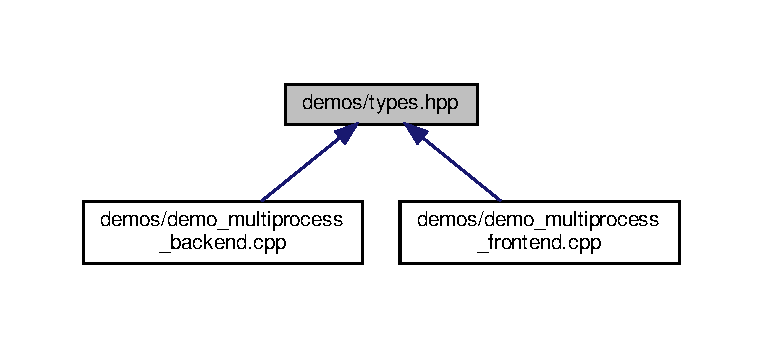
\includegraphics[width=350pt]{demos_2types_8hpp__dep__incl}
\end{center}
\end{figure}
\subsection*{Classes}
\begin{DoxyCompactItemize}
\item 
class \hyperlink{classrobot__interfaces_1_1demo_1_1Action}{robot\+\_\+interfaces\+::demo\+::\+Action}
\begin{DoxyCompactList}\small\item\em Actions to be performed by robot, will be received by \hyperlink{classDriver}{Driver}. \end{DoxyCompactList}\item 
class \hyperlink{classrobot__interfaces_1_1demo_1_1Observation}{robot\+\_\+interfaces\+::demo\+::\+Observation}
\begin{DoxyCompactList}\small\item\em Read from the robot by \hyperlink{classDriver}{Driver}. \end{DoxyCompactList}\end{DoxyCompactItemize}


\subsection{Detailed Description}
license License B\+S\+D-\/3-\/\+Clause 

\begin{DoxyCopyright}{Copyright}
Copyright (c) 2019-\/2020, Max Planck Gesellschaft.
\end{DoxyCopyright}
Simple Action and Observation types that are used by some demos. 
\hypertarget{include_2robot__interfaces_2types_8hpp}{}\section{include/robot\+\_\+interfaces/types.hpp File Reference}
\label{include_2robot__interfaces_2types_8hpp}\index{include/robot\+\_\+interfaces/types.\+hpp@{include/robot\+\_\+interfaces/types.\+hpp}}


Observation of a Finger robot.  


{\ttfamily \#include $<$memory$>$}\newline
{\ttfamily \#include \char`\"{}robot\+\_\+backend.\+hpp\char`\"{}}\newline
{\ttfamily \#include \char`\"{}robot\+\_\+data.\+hpp\char`\"{}}\newline
{\ttfamily \#include \char`\"{}robot\+\_\+frontend.\+hpp\char`\"{}}\newline
{\ttfamily \#include \char`\"{}robot\+\_\+logger.\+hpp\char`\"{}}\newline
Include dependency graph for types.\+hpp\+:
\nopagebreak
\begin{figure}[H]
\begin{center}
\leavevmode
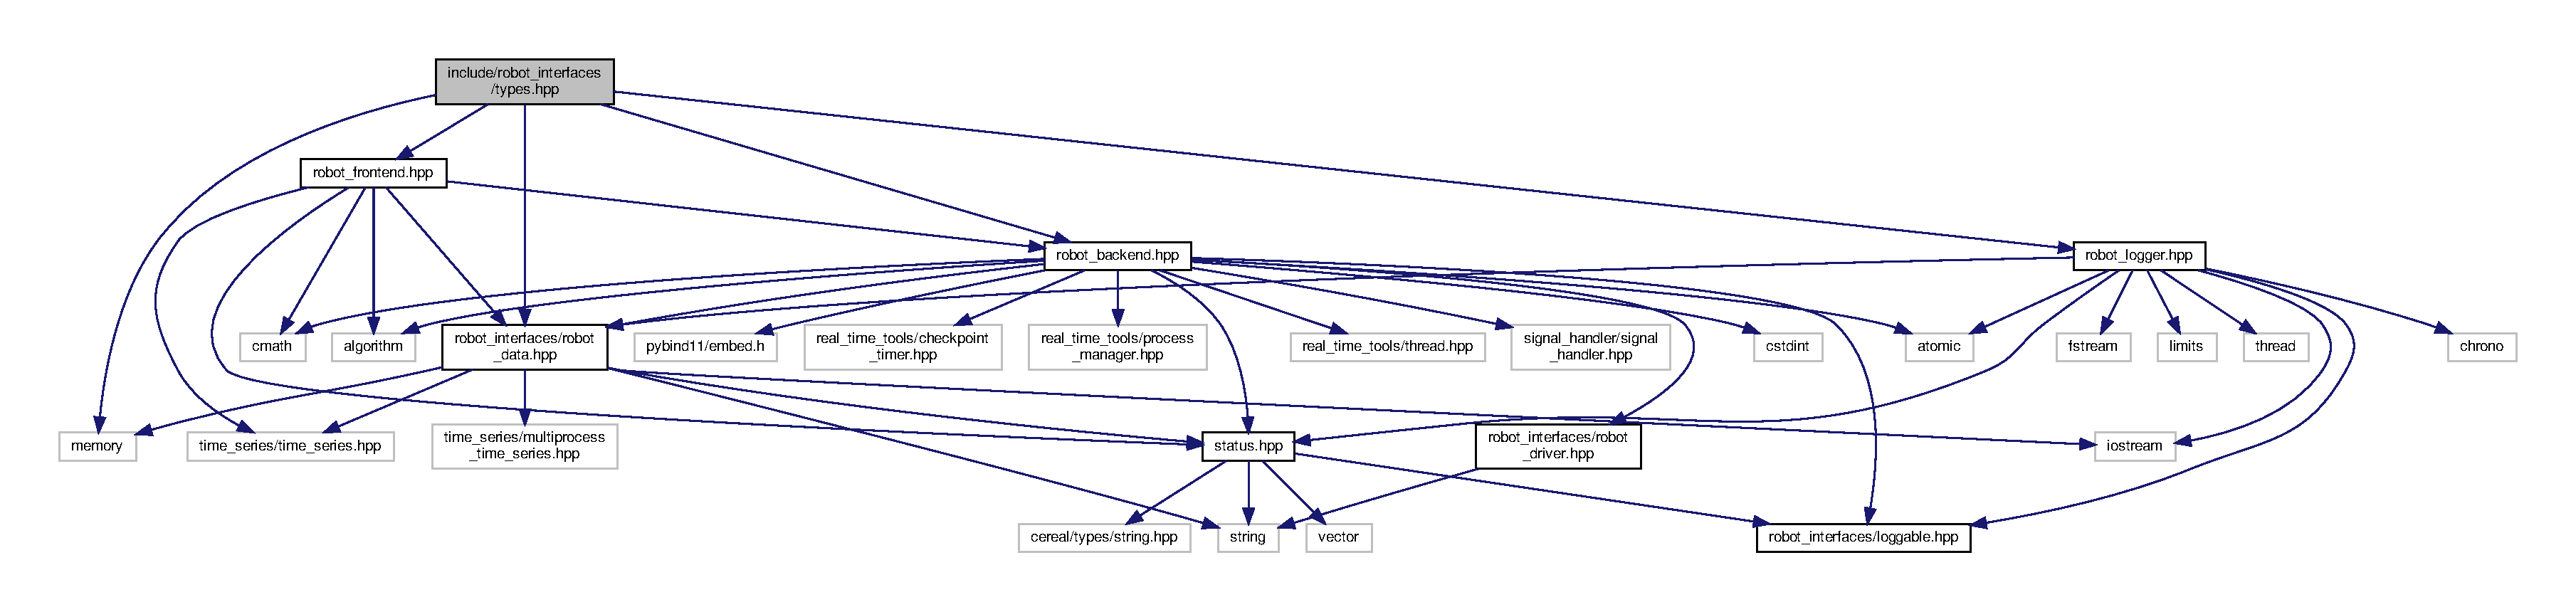
\includegraphics[width=350pt]{include_2robot__interfaces_2types_8hpp__incl}
\end{center}
\end{figure}
This graph shows which files directly or indirectly include this file\+:
\nopagebreak
\begin{figure}[H]
\begin{center}
\leavevmode
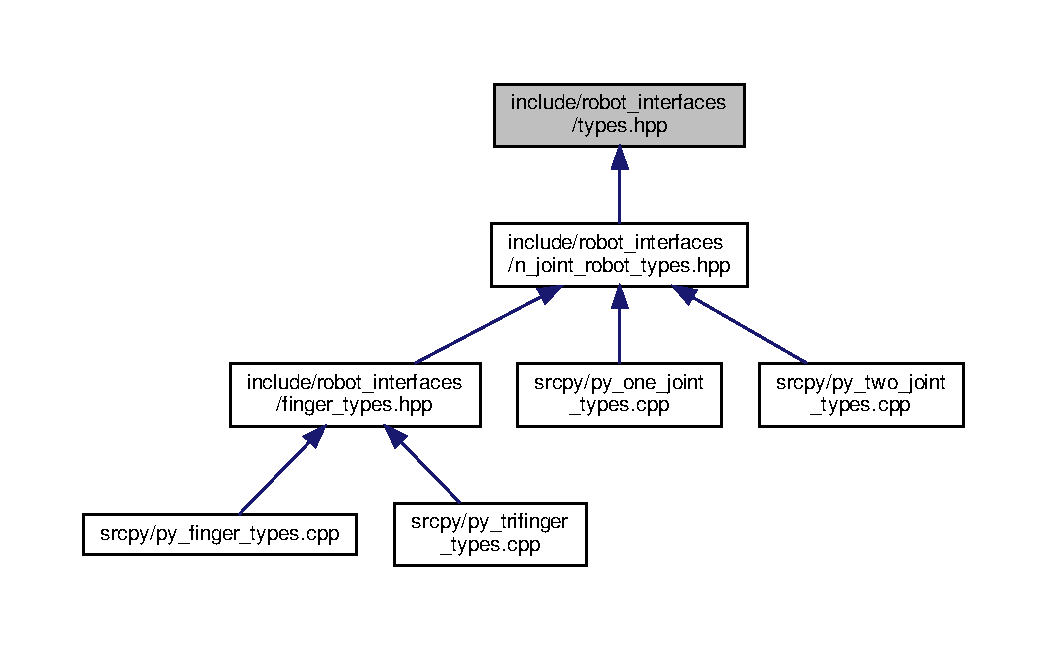
\includegraphics[width=350pt]{include_2robot__interfaces_2types_8hpp__dep__incl}
\end{center}
\end{figure}
\subsection*{Classes}
\begin{DoxyCompactItemize}
\item 
struct \hyperlink{structrobot__interfaces_1_1RobotInterfaceTypes}{robot\+\_\+interfaces\+::\+Robot\+Interface\+Types$<$ Action\+\_\+t, Observation\+\_\+t $>$}
\end{DoxyCompactItemize}


\subsection{Detailed Description}
Observation of a Finger robot. 

\begin{DoxyCopyright}{Copyright}
2020, Max Planck Gesellschaft. All rights reserved. 
\end{DoxyCopyright}
\begin{DoxyRefDesc}{License}
\item[\hyperlink{license__license000012}{License}]B\+SD 3-\/clause \end{DoxyRefDesc}

\hypertarget{example_8hpp}{}\section{include/robot\+\_\+interfaces/example.hpp File Reference}
\label{example_8hpp}\index{include/robot\+\_\+interfaces/example.\+hpp@{include/robot\+\_\+interfaces/example.\+hpp}}


license License B\+S\+D-\/3-\/\+Clause  


{\ttfamily \#include $<$unistd.\+h$>$}\newline
{\ttfamily \#include $<$iostream$>$}\newline
{\ttfamily \#include $<$robot\+\_\+interfaces/robot\+\_\+driver.\+hpp$>$}\newline
Include dependency graph for example.\+hpp\+:
\nopagebreak
\begin{figure}[H]
\begin{center}
\leavevmode
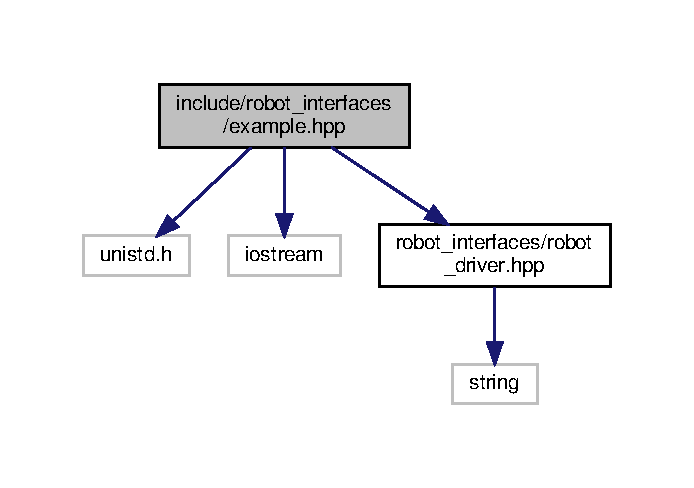
\includegraphics[width=333pt]{example_8hpp__incl}
\end{center}
\end{figure}
This graph shows which files directly or indirectly include this file\+:
\nopagebreak
\begin{figure}[H]
\begin{center}
\leavevmode
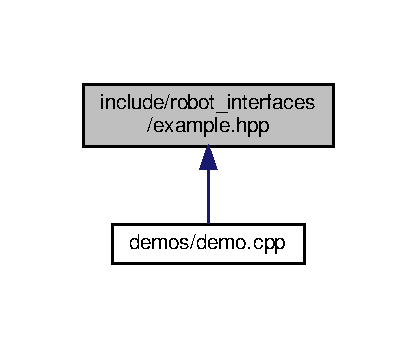
\includegraphics[width=200pt]{example_8hpp__dep__incl}
\end{center}
\end{figure}
\subsection*{Classes}
\begin{DoxyCompactItemize}
\item 
class \hyperlink{classrobot__interfaces_1_1example_1_1Action}{robot\+\_\+interfaces\+::example\+::\+Action}
\begin{DoxyCompactList}\small\item\em Actions to be performed by robot, will be received by \hyperlink{classrobot__interfaces_1_1example_1_1Driver}{Driver}. \end{DoxyCompactList}\item 
class \hyperlink{classrobot__interfaces_1_1example_1_1Observation}{robot\+\_\+interfaces\+::example\+::\+Observation}
\begin{DoxyCompactList}\small\item\em \hyperlink{classrobot__interfaces_1_1example_1_1Observation}{Observation} read from the robot by \hyperlink{classrobot__interfaces_1_1example_1_1Driver}{Driver}. \end{DoxyCompactList}\item 
class \hyperlink{classrobot__interfaces_1_1example_1_1Driver}{robot\+\_\+interfaces\+::example\+::\+Driver}
\begin{DoxyCompactList}\small\item\em Example \hyperlink{classrobot__interfaces_1_1Robot}{Robot} \hyperlink{classrobot__interfaces_1_1example_1_1Driver}{Driver}. \end{DoxyCompactList}\end{DoxyCompactItemize}


\subsection{Detailed Description}
license License B\+S\+D-\/3-\/\+Clause 

\begin{DoxyCopyright}{Copyright}
Copyright (c) 2019, Max Planck Gesellschaft.
\end{DoxyCopyright}
Example driver and types for demo and testing purposes. 
\hypertarget{n__finger__observation_8hpp}{}\section{include/robot\+\_\+interfaces/n\+\_\+finger\+\_\+observation.hpp File Reference}
\label{n__finger__observation_8hpp}\index{include/robot\+\_\+interfaces/n\+\_\+finger\+\_\+observation.\+hpp@{include/robot\+\_\+interfaces/n\+\_\+finger\+\_\+observation.\+hpp}}


Observation of a Finger robot.  


{\ttfamily \#include $<$string$>$}\newline
{\ttfamily \#include $<$vector$>$}\newline
{\ttfamily \#include $<$Eigen/\+Eigen$>$}\newline
{\ttfamily \#include $<$serialization\+\_\+utils/cereal\+\_\+eigen.\+hpp$>$}\newline
{\ttfamily \#include $<$robot\+\_\+interfaces/loggable.\+hpp$>$}\newline
Include dependency graph for n\+\_\+finger\+\_\+observation.\+hpp\+:
\nopagebreak
\begin{figure}[H]
\begin{center}
\leavevmode
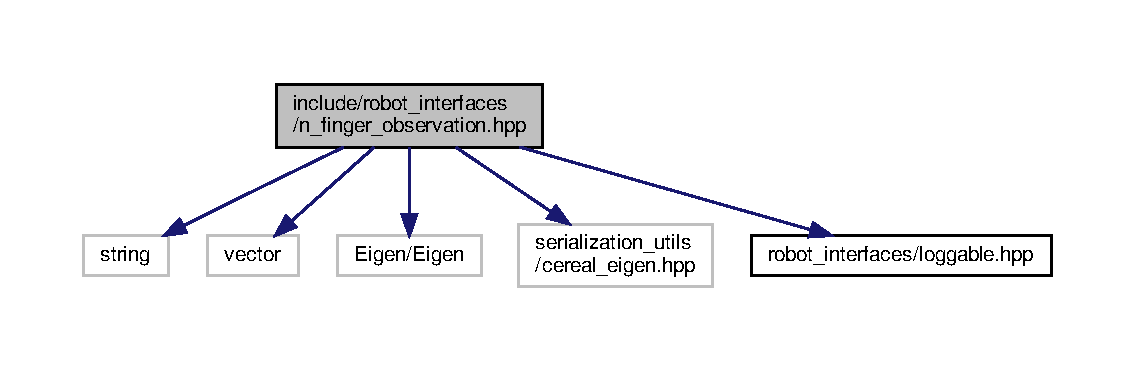
\includegraphics[width=350pt]{n__finger__observation_8hpp__incl}
\end{center}
\end{figure}
This graph shows which files directly or indirectly include this file\+:
\nopagebreak
\begin{figure}[H]
\begin{center}
\leavevmode
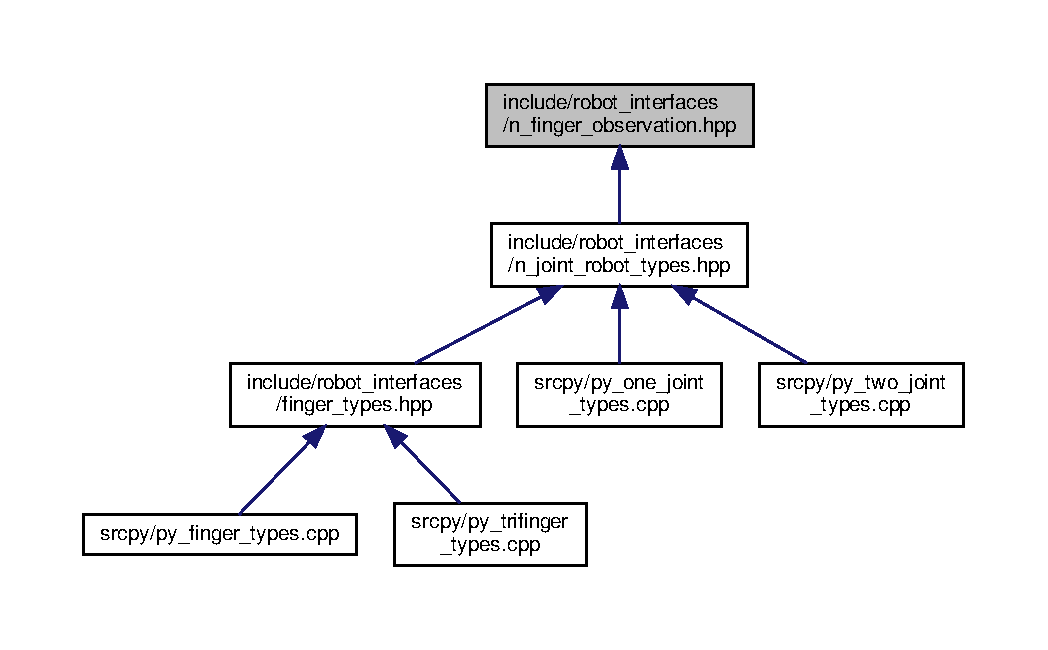
\includegraphics[width=350pt]{n__finger__observation_8hpp__dep__incl}
\end{center}
\end{figure}
\subsection*{Classes}
\begin{DoxyCompactItemize}
\item 
struct \hyperlink{structrobot__interfaces_1_1NFingerObservation}{robot\+\_\+interfaces\+::\+N\+Finger\+Observation$<$ N\+\_\+\+F\+I\+N\+G\+E\+R\+S $>$}
\begin{DoxyCompactList}\small\item\em Observation of a Finger robot. \end{DoxyCompactList}\end{DoxyCompactItemize}


\subsection{Detailed Description}
Observation of a Finger robot. 

\begin{DoxyCopyright}{Copyright}
2020, Max Planck Gesellschaft. All rights reserved. 
\end{DoxyCopyright}
\begin{DoxyRefDesc}{License}
\item[\hyperlink{license__license000001}{License}]B\+SD 3-\/clause \end{DoxyRefDesc}

\hypertarget{n__joint__action_8hpp}{}\section{include/robot\+\_\+interfaces/n\+\_\+joint\+\_\+action.hpp File Reference}
\label{n__joint__action_8hpp}\index{include/robot\+\_\+interfaces/n\+\_\+joint\+\_\+action.\+hpp@{include/robot\+\_\+interfaces/n\+\_\+joint\+\_\+action.\+hpp}}


Action of a generic n-\/joint robot.  


{\ttfamily \#include $<$limits$>$}\newline
{\ttfamily \#include $<$string$>$}\newline
{\ttfamily \#include $<$vector$>$}\newline
{\ttfamily \#include $<$Eigen/\+Eigen$>$}\newline
{\ttfamily \#include $<$serialization\+\_\+utils/cereal\+\_\+eigen.\+hpp$>$}\newline
{\ttfamily \#include $<$robot\+\_\+interfaces/loggable.\+hpp$>$}\newline
Include dependency graph for n\+\_\+joint\+\_\+action.\+hpp\+:
\nopagebreak
\begin{figure}[H]
\begin{center}
\leavevmode
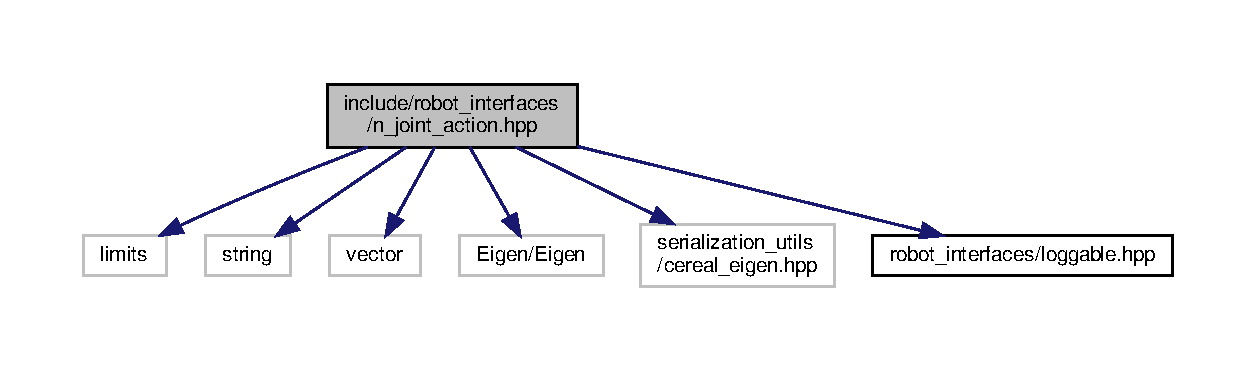
\includegraphics[width=350pt]{n__joint__action_8hpp__incl}
\end{center}
\end{figure}
This graph shows which files directly or indirectly include this file\+:
\nopagebreak
\begin{figure}[H]
\begin{center}
\leavevmode
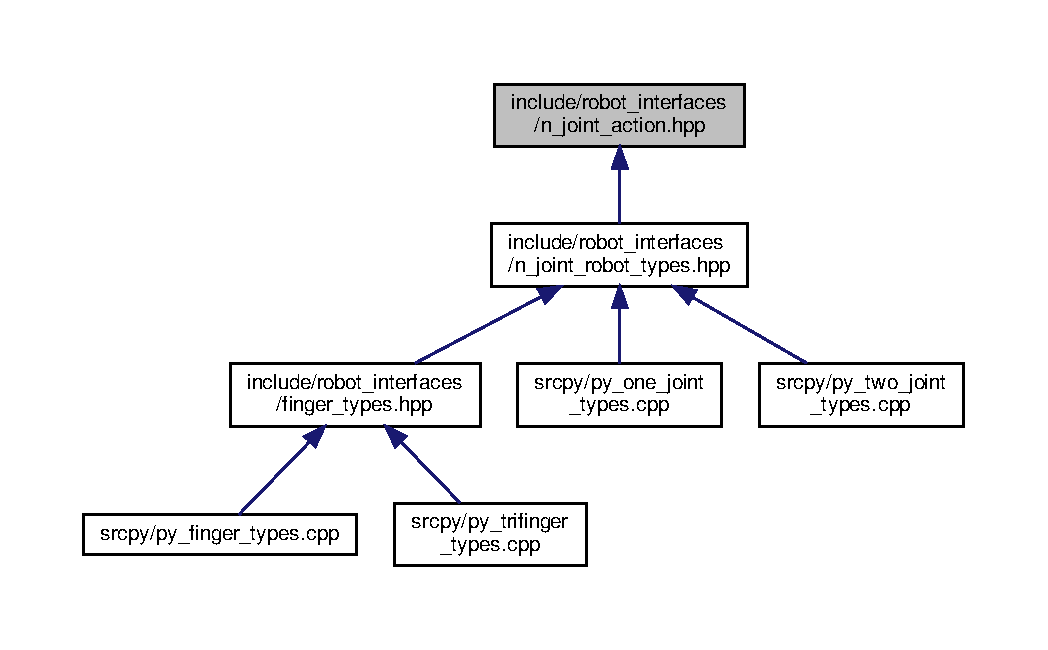
\includegraphics[width=350pt]{n__joint__action_8hpp__dep__incl}
\end{center}
\end{figure}
\subsection*{Classes}
\begin{DoxyCompactItemize}
\item 
struct \hyperlink{structrobot__interfaces_1_1NJointAction}{robot\+\_\+interfaces\+::\+N\+Joint\+Action$<$ N $>$}
\begin{DoxyCompactList}\small\item\em Action of a generic n-\/joint robot. \end{DoxyCompactList}\end{DoxyCompactItemize}


\subsection{Detailed Description}
Action of a generic n-\/joint robot. 

\begin{DoxyCopyright}{Copyright}
2020, Max Planck Gesellschaft. All rights reserved. 
\end{DoxyCopyright}
\begin{DoxyRefDesc}{License}
\item[\hyperlink{license__license000002}{License}]B\+SD 3-\/clause \end{DoxyRefDesc}

\hypertarget{n__joint__observation_8hpp}{}\section{include/robot\+\_\+interfaces/n\+\_\+joint\+\_\+observation.hpp File Reference}
\label{n__joint__observation_8hpp}\index{include/robot\+\_\+interfaces/n\+\_\+joint\+\_\+observation.\+hpp@{include/robot\+\_\+interfaces/n\+\_\+joint\+\_\+observation.\+hpp}}


Observation of a generic n-\/joint robot.  


{\ttfamily \#include $<$string$>$}\newline
{\ttfamily \#include $<$vector$>$}\newline
{\ttfamily \#include $<$Eigen/\+Eigen$>$}\newline
{\ttfamily \#include $<$serialization\+\_\+utils/cereal\+\_\+eigen.\+hpp$>$}\newline
{\ttfamily \#include $<$robot\+\_\+interfaces/loggable.\+hpp$>$}\newline
Include dependency graph for n\+\_\+joint\+\_\+observation.\+hpp\+:
\nopagebreak
\begin{figure}[H]
\begin{center}
\leavevmode
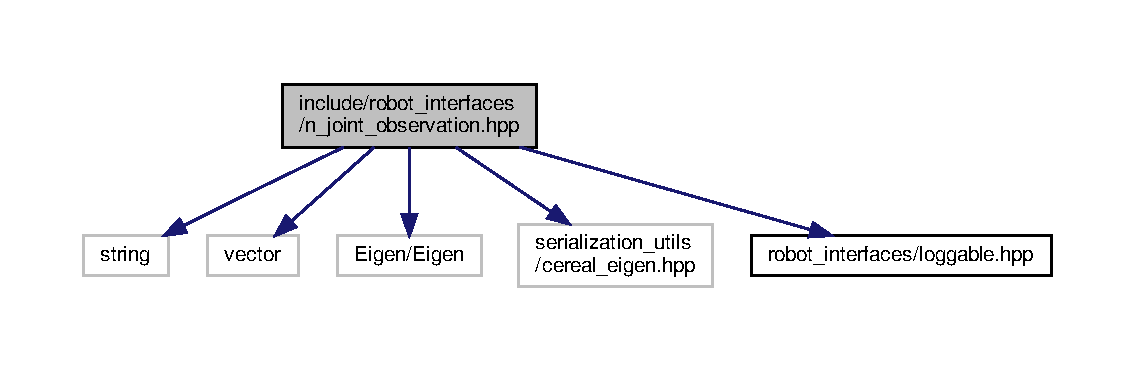
\includegraphics[width=350pt]{n__joint__observation_8hpp__incl}
\end{center}
\end{figure}
This graph shows which files directly or indirectly include this file\+:
\nopagebreak
\begin{figure}[H]
\begin{center}
\leavevmode
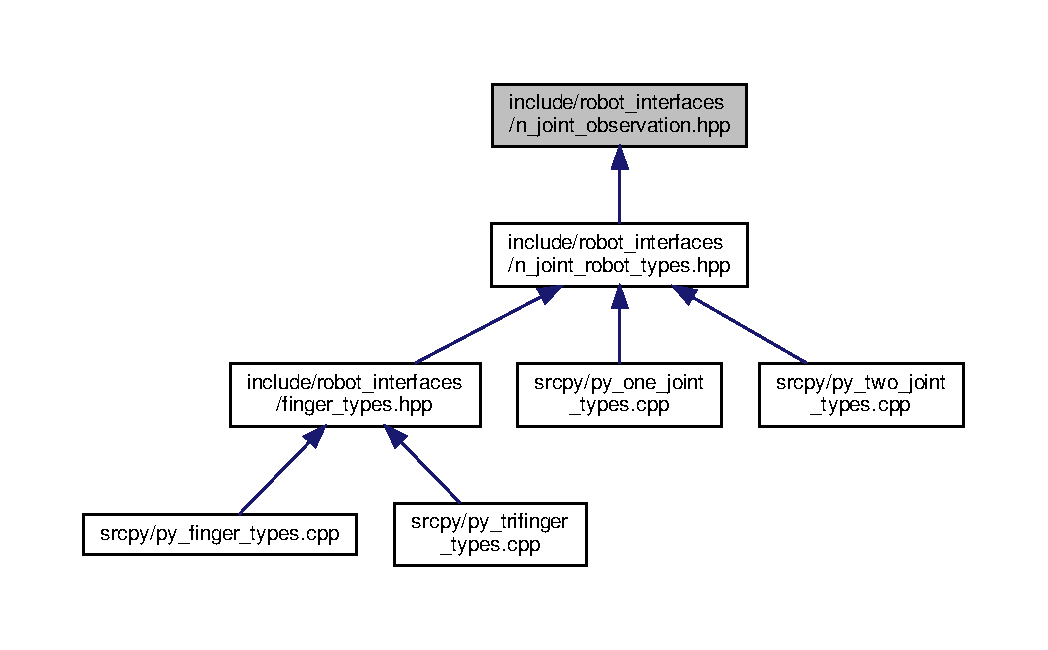
\includegraphics[width=350pt]{n__joint__observation_8hpp__dep__incl}
\end{center}
\end{figure}
\subsection*{Classes}
\begin{DoxyCompactItemize}
\item 
struct \hyperlink{structrobot__interfaces_1_1NJointObservation}{robot\+\_\+interfaces\+::\+N\+Joint\+Observation$<$ N $>$}
\begin{DoxyCompactList}\small\item\em Basic observation for a generic n-\/joint robot. \end{DoxyCompactList}\end{DoxyCompactItemize}


\subsection{Detailed Description}
Observation of a generic n-\/joint robot. 

\begin{DoxyCopyright}{Copyright}
2020, Max Planck Gesellschaft. All rights reserved. 
\end{DoxyCopyright}
\begin{DoxyRefDesc}{License}
\item[\hyperlink{license__license000003}{License}]B\+SD 3-\/clause \end{DoxyRefDesc}

\hypertarget{n__joint__robot__types_8hpp}{}\section{include/robot\+\_\+interfaces/n\+\_\+joint\+\_\+robot\+\_\+types.hpp File Reference}
\label{n__joint__robot__types_8hpp}\index{include/robot\+\_\+interfaces/n\+\_\+joint\+\_\+robot\+\_\+types.\+hpp@{include/robot\+\_\+interfaces/n\+\_\+joint\+\_\+robot\+\_\+types.\+hpp}}


Types for an n-\/joint robot.  


{\ttfamily \#include \char`\"{}n\+\_\+finger\+\_\+observation.\+hpp\char`\"{}}\newline
{\ttfamily \#include \char`\"{}n\+\_\+joint\+\_\+action.\+hpp\char`\"{}}\newline
{\ttfamily \#include \char`\"{}n\+\_\+joint\+\_\+observation.\+hpp\char`\"{}}\newline
{\ttfamily \#include \char`\"{}types.\+hpp\char`\"{}}\newline
Include dependency graph for n\+\_\+joint\+\_\+robot\+\_\+types.\+hpp\+:
\nopagebreak
\begin{figure}[H]
\begin{center}
\leavevmode
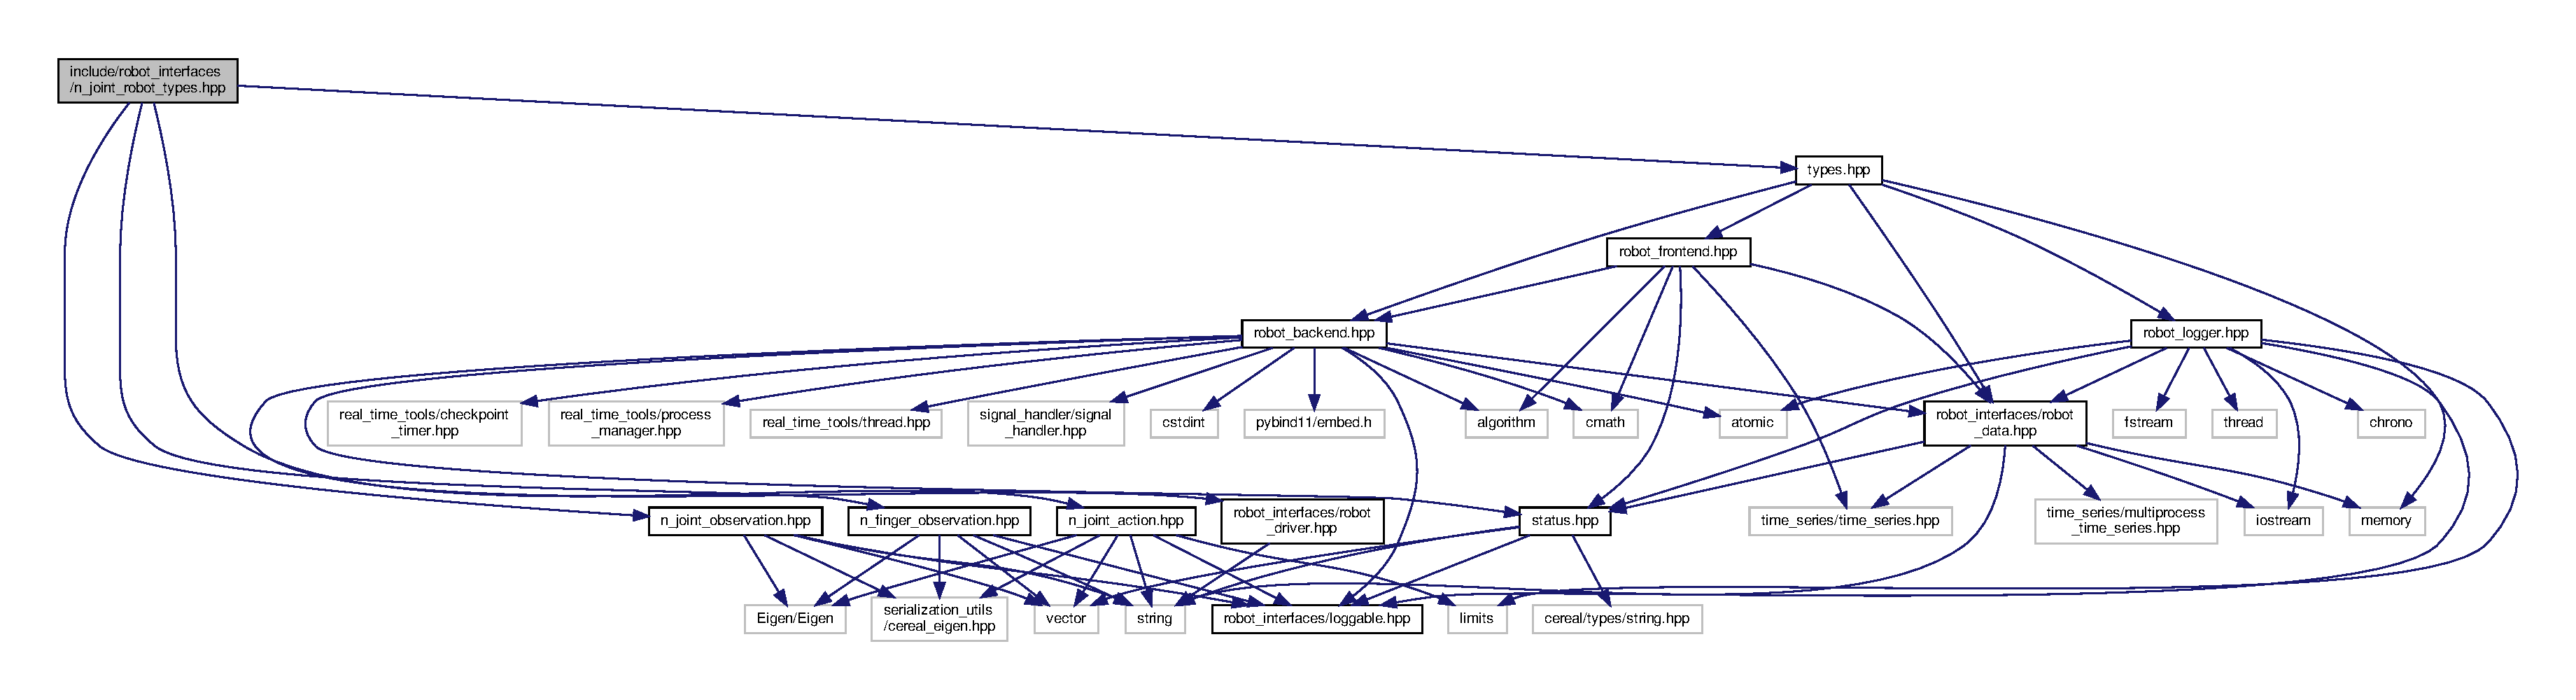
\includegraphics[width=350pt]{n__joint__robot__types_8hpp__incl}
\end{center}
\end{figure}
This graph shows which files directly or indirectly include this file\+:
\nopagebreak
\begin{figure}[H]
\begin{center}
\leavevmode
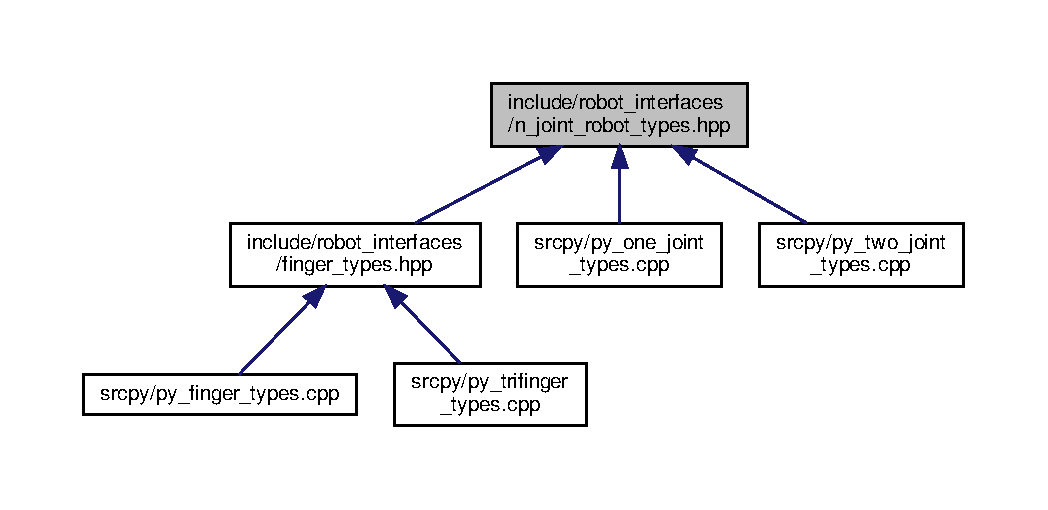
\includegraphics[width=350pt]{n__joint__robot__types_8hpp__dep__incl}
\end{center}
\end{figure}
\subsection*{Classes}
\begin{DoxyCompactItemize}
\item 
struct \hyperlink{structrobot__interfaces_1_1SimpleNJointRobotTypes}{robot\+\_\+interfaces\+::\+Simple\+N\+Joint\+Robot\+Types$<$ N $>$}
\begin{DoxyCompactList}\small\item\em Collection of types for a generic N-\/joint B\+L\+MC robot. \end{DoxyCompactList}\end{DoxyCompactItemize}


\subsection{Detailed Description}
Types for an n-\/joint robot. 

\begin{DoxyCopyright}{Copyright}
2020, Max Planck Gesellschaft. All rights reserved. 
\end{DoxyCopyright}
\begin{DoxyRefDesc}{License}
\item[\hyperlink{license__license000004}{License}]B\+SD 3-\/clause \end{DoxyRefDesc}

\hypertarget{pybind__helper_8hpp}{}\section{include/robot\+\_\+interfaces/pybind\+\_\+helper.hpp File Reference}
\label{pybind__helper_8hpp}\index{include/robot\+\_\+interfaces/pybind\+\_\+helper.\+hpp@{include/robot\+\_\+interfaces/pybind\+\_\+helper.\+hpp}}


Helper functions for creating Python bindings.  


{\ttfamily \#include $<$type\+\_\+traits$>$}\newline
{\ttfamily \#include $<$pybind11/eigen.\+h$>$}\newline
{\ttfamily \#include $<$pybind11/pybind11.\+h$>$}\newline
{\ttfamily \#include $<$pybind11/stl\+\_\+bind.\+h$>$}\newline
{\ttfamily \#include $<$robot\+\_\+interfaces/robot\+\_\+frontend.\+hpp$>$}\newline
Include dependency graph for pybind\+\_\+helper.\+hpp\+:
\nopagebreak
\begin{figure}[H]
\begin{center}
\leavevmode
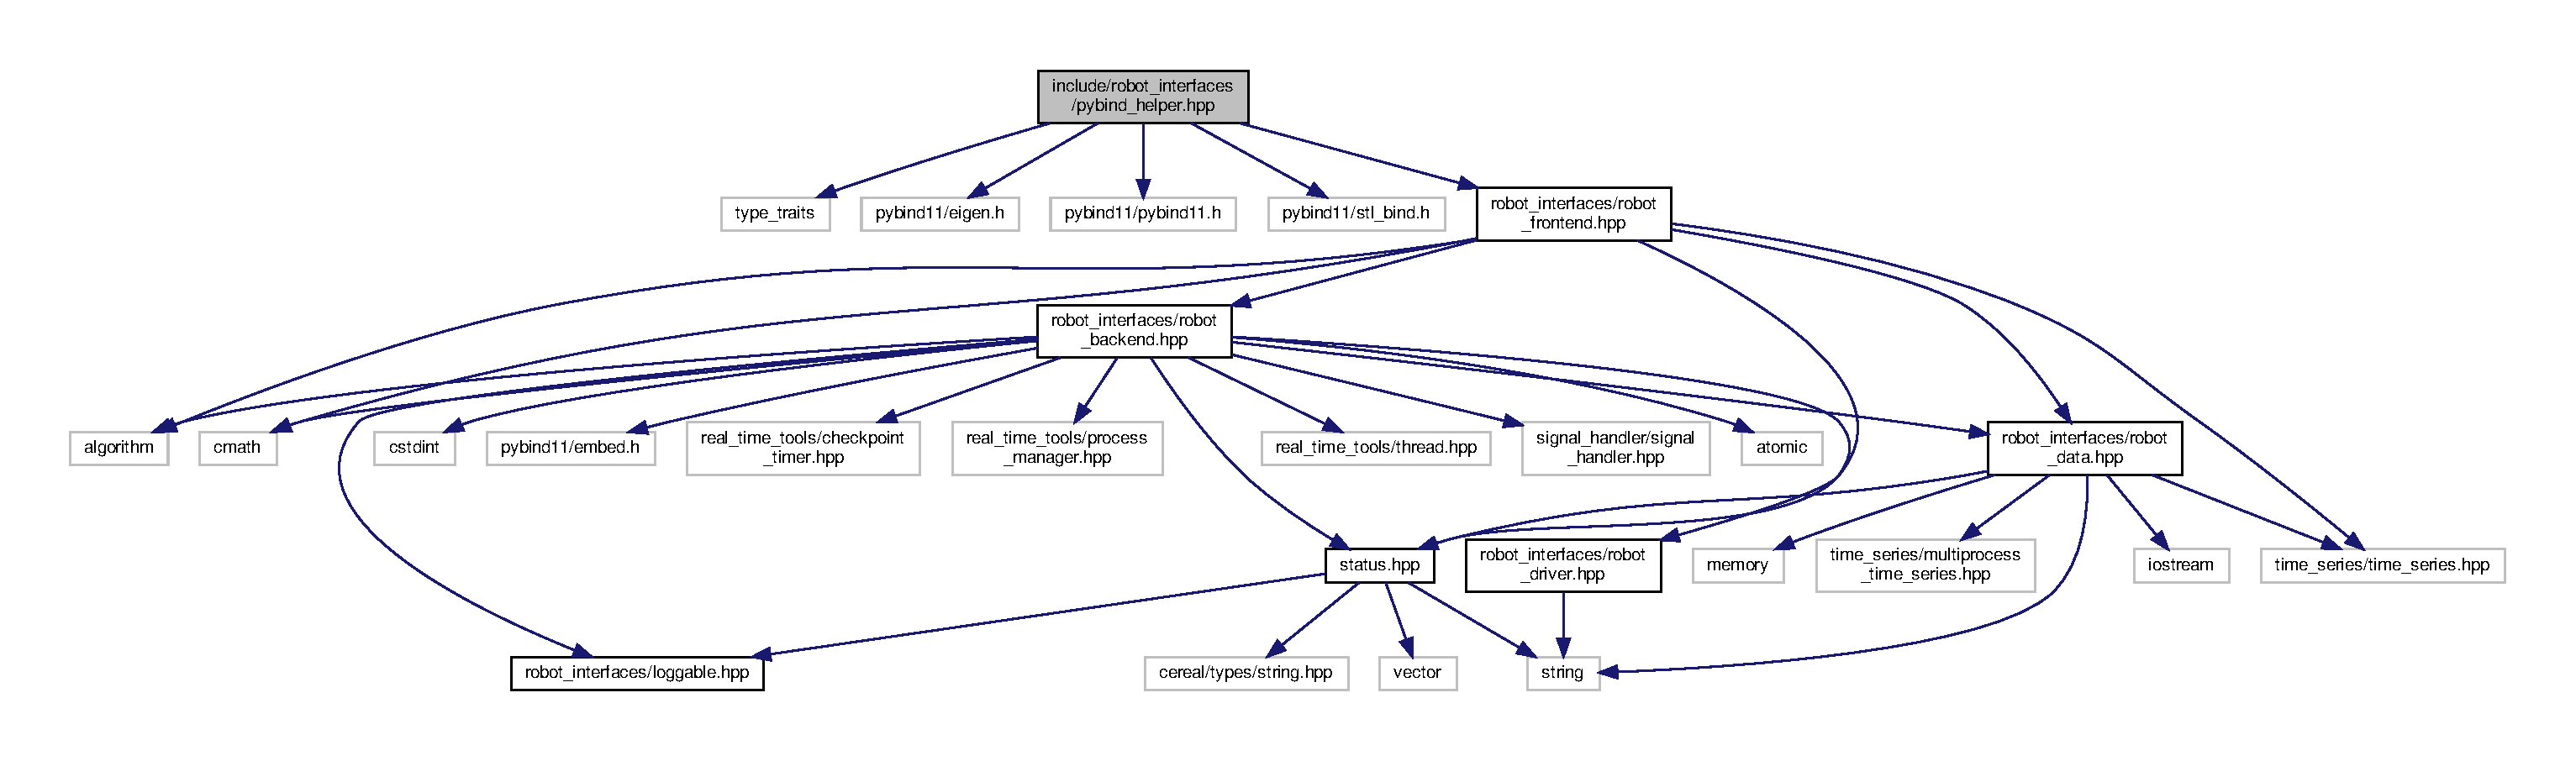
\includegraphics[width=350pt]{pybind__helper_8hpp__incl}
\end{center}
\end{figure}
This graph shows which files directly or indirectly include this file\+:
\nopagebreak
\begin{figure}[H]
\begin{center}
\leavevmode
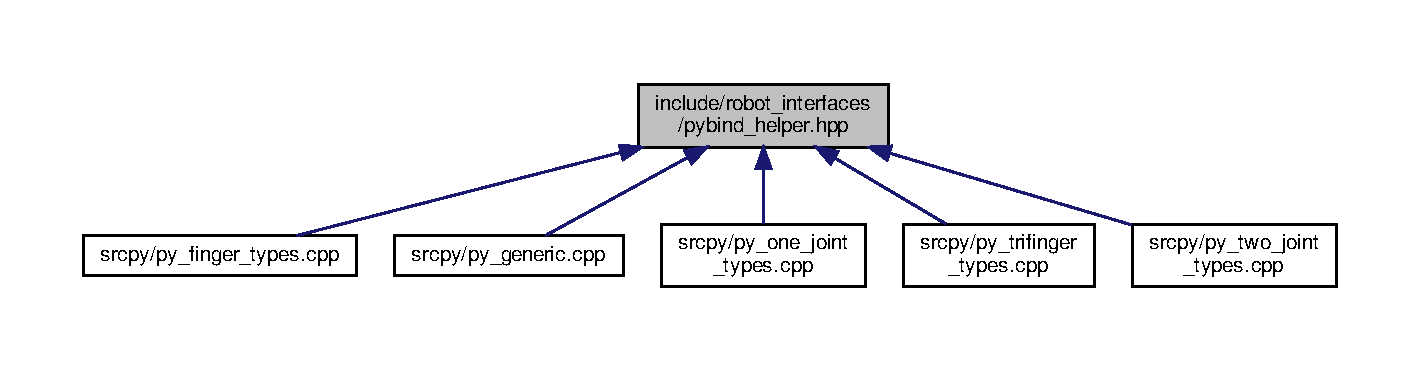
\includegraphics[width=350pt]{pybind__helper_8hpp__dep__incl}
\end{center}
\end{figure}
\subsection*{Classes}
\begin{DoxyCompactItemize}
\item 
struct \hyperlink{structrobot__interfaces_1_1BindTipForceIfExists}{robot\+\_\+interfaces\+::\+Bind\+Tip\+Force\+If\+Exists$<$ Types, typename $>$}
\begin{DoxyCompactList}\small\item\em Add Python bindings for Types\+::\+Observaton\+::tip\+\_\+force if it exists. \end{DoxyCompactList}\item 
struct \hyperlink{structrobot__interfaces_1_1BindTipForceIfExists_3_01Types_00_01decltype_07_07void_08_01Types_1_14cbc6933c476f63b7bfd2943748e44ea}{robot\+\_\+interfaces\+::\+Bind\+Tip\+Force\+If\+Exists$<$ Types, decltype((void) Types\+::\+Observation\+::tip\+\_\+force, 0)$>$}
\end{DoxyCompactItemize}
\subsection*{Functions}
\begin{DoxyCompactItemize}
\item 
{\footnotesize template$<$typename Types $>$ }\\void \hyperlink{pybind__helper_8hpp_a82052567130c3000eeef9f5520885233}{robot\+\_\+interfaces\+::create\+\_\+python\+\_\+bindings} (pybind11\+::module \&m)
\begin{DoxyCompactList}\small\item\em Create Python bindings for the specified robot Types. \end{DoxyCompactList}\end{DoxyCompactItemize}


\subsection{Detailed Description}
Helper functions for creating Python bindings. 



\subsection{Function Documentation}
\mbox{\Hypertarget{pybind__helper_8hpp_file_a82052567130c3000eeef9f5520885233}\label{pybind__helper_8hpp_file_a82052567130c3000eeef9f5520885233}} 
\index{pybind\+\_\+helper.\+hpp@{pybind\+\_\+helper.\+hpp}!create\+\_\+python\+\_\+bindings@{create\+\_\+python\+\_\+bindings}}
\index{create\+\_\+python\+\_\+bindings@{create\+\_\+python\+\_\+bindings}!pybind\+\_\+helper.\+hpp@{pybind\+\_\+helper.\+hpp}}
\subsubsection{\texorpdfstring{create\+\_\+python\+\_\+bindings()}{create\_python\_bindings()}}
{\footnotesize\ttfamily template$<$typename Types $>$ \\
void robot\+\_\+interfaces\+::create\+\_\+python\+\_\+bindings (\begin{DoxyParamCaption}\item[{pybind11\+::module \&}]{m }\end{DoxyParamCaption})}



Create Python bindings for the specified robot Types. 

With this function, Python bindings can easily be created for new robots that are based on the N\+Joint\+Robot\+Types. Example\+: \begin{DoxyVerb}PYBIND11_MODULE(py_fortytwo_types, m)
{
    create_python_bindings<NJointRobotTypes<42>>(m);
}
\end{DoxyVerb}



\begin{DoxyTemplParams}{Template Parameters}
{\em Types} & An instance of N\+Joint\+Robot\+Types. \\
\hline
\end{DoxyTemplParams}

\begin{DoxyParams}{Parameters}
{\em m} & The second argument of the P\+Y\+B\+I\+N\+D11\+\_\+\+M\+O\+D\+U\+LE macro. \\
\hline
\end{DoxyParams}

\hypertarget{robot__data_8hpp}{}\section{include/robot\+\_\+interfaces/robot\+\_\+data.hpp File Reference}
\label{robot__data_8hpp}\index{include/robot\+\_\+interfaces/robot\+\_\+data.\+hpp@{include/robot\+\_\+interfaces/robot\+\_\+data.\+hpp}}


Robot\+Data classes for both single-\/ and multi-\/process applications.  


{\ttfamily \#include $<$iostream$>$}\newline
{\ttfamily \#include $<$memory$>$}\newline
{\ttfamily \#include $<$string$>$}\newline
{\ttfamily \#include $<$time\+\_\+series/multiprocess\+\_\+time\+\_\+series.\+hpp$>$}\newline
{\ttfamily \#include $<$time\+\_\+series/time\+\_\+series.\+hpp$>$}\newline
{\ttfamily \#include \char`\"{}status.\+hpp\char`\"{}}\newline
Include dependency graph for robot\+\_\+data.\+hpp\+:
\nopagebreak
\begin{figure}[H]
\begin{center}
\leavevmode
\includegraphics[width=350pt]{robot__data_8hpp__incl}
\end{center}
\end{figure}
This graph shows which files directly or indirectly include this file\+:
\nopagebreak
\begin{figure}[H]
\begin{center}
\leavevmode
\includegraphics[width=350pt]{robot__data_8hpp__dep__incl}
\end{center}
\end{figure}
\subsection*{Classes}
\begin{DoxyCompactItemize}
\item 
class \hyperlink{classrobot__interfaces_1_1RobotData}{robot\+\_\+interfaces\+::\+Robot\+Data$<$ Action, Observation $>$}
\begin{DoxyCompactList}\small\item\em Contains all the input and output data of the robot. \end{DoxyCompactList}\item 
class \hyperlink{classrobot__interfaces_1_1SingleProcessRobotData}{robot\+\_\+interfaces\+::\+Single\+Process\+Robot\+Data$<$ Action, Observation $>$}
\begin{DoxyCompactList}\small\item\em \hyperlink{classrobot__interfaces_1_1RobotData}{Robot\+Data} instance using single process time series. \end{DoxyCompactList}\item 
class \hyperlink{classrobot__interfaces_1_1MultiProcessRobotData}{robot\+\_\+interfaces\+::\+Multi\+Process\+Robot\+Data$<$ Action, Observation $>$}
\begin{DoxyCompactList}\small\item\em \hyperlink{classrobot__interfaces_1_1RobotData}{Robot\+Data} instance using multi process time series. \end{DoxyCompactList}\end{DoxyCompactItemize}


\subsection{Detailed Description}
Robot\+Data classes for both single-\/ and multi-\/process applications. 

\begin{DoxyRefDesc}{License}
\item[\hyperlink{license__license000005}{License}]B\+SD 3-\/clause \end{DoxyRefDesc}
\begin{DoxyCopyright}{Copyright}
Copyright (c) 2018-\/2020, New York University and Max Planck Gesellschaft 
\end{DoxyCopyright}

\hypertarget{pybind__sensors_8hpp}{}\section{include/robot\+\_\+interfaces/sensors/pybind\+\_\+sensors.hpp File Reference}
\label{pybind__sensors_8hpp}\index{include/robot\+\_\+interfaces/sensors/pybind\+\_\+sensors.\+hpp@{include/robot\+\_\+interfaces/sensors/pybind\+\_\+sensors.\+hpp}}


Binds methods and objects to enable access from python.  


{\ttfamily \#include $<$pybind11/eigen.\+h$>$}\newline
{\ttfamily \#include $<$pybind11/pybind11.\+h$>$}\newline
{\ttfamily \#include $<$pybind11/stl.\+h$>$}\newline
{\ttfamily \#include $<$robot\+\_\+interfaces/sensors/sensor\+\_\+backend.\+hpp$>$}\newline
{\ttfamily \#include $<$robot\+\_\+interfaces/sensors/sensor\+\_\+data.\+hpp$>$}\newline
{\ttfamily \#include $<$robot\+\_\+interfaces/sensors/sensor\+\_\+driver.\+hpp$>$}\newline
{\ttfamily \#include $<$robot\+\_\+interfaces/sensors/sensor\+\_\+frontend.\+hpp$>$}\newline
{\ttfamily \#include $<$robot\+\_\+interfaces/sensors/sensor\+\_\+log\+\_\+reader.\+hpp$>$}\newline
{\ttfamily \#include $<$robot\+\_\+interfaces/sensors/sensor\+\_\+logger.\+hpp$>$}\newline
Include dependency graph for pybind\+\_\+sensors.\+hpp\+:
\nopagebreak
\begin{figure}[H]
\begin{center}
\leavevmode
\includegraphics[width=350pt]{pybind__sensors_8hpp__incl}
\end{center}
\end{figure}
\subsection*{Functions}
\begin{DoxyCompactItemize}
\item 
{\footnotesize template$<$typename Observation\+Type $>$ }\\void \hyperlink{pybind__sensors_8hpp_a31fc2ebe96b63e949a14f3f08cfea9b4}{robot\+\_\+interfaces\+::create\+\_\+sensor\+\_\+bindings} (pybind11\+::module \&m)
\begin{DoxyCompactList}\small\item\em Create python bindings for different sensor types. \end{DoxyCompactList}\end{DoxyCompactItemize}


\subsection{Detailed Description}
Binds methods and objects to enable access from python. 

\begin{DoxyCopyright}{Copyright}
2020, New York University, Max Planck Gesellschaft. All rights reserved. 
\end{DoxyCopyright}
\begin{DoxyRefDesc}{License}
\item[\hyperlink{license__license000006}{License}]B\+SD 3-\/clause \end{DoxyRefDesc}


\subsection{Function Documentation}
\mbox{\Hypertarget{pybind__sensors_8hpp_file_a31fc2ebe96b63e949a14f3f08cfea9b4}\label{pybind__sensors_8hpp_file_a31fc2ebe96b63e949a14f3f08cfea9b4}} 
\index{pybind\+\_\+sensors.\+hpp@{pybind\+\_\+sensors.\+hpp}!create\+\_\+sensor\+\_\+bindings@{create\+\_\+sensor\+\_\+bindings}}
\index{create\+\_\+sensor\+\_\+bindings@{create\+\_\+sensor\+\_\+bindings}!pybind\+\_\+sensors.\+hpp@{pybind\+\_\+sensors.\+hpp}}
\subsubsection{\texorpdfstring{create\+\_\+sensor\+\_\+bindings()}{create\_sensor\_bindings()}}
{\footnotesize\ttfamily template$<$typename Observation\+Type $>$ \\
void robot\+\_\+interfaces\+::create\+\_\+sensor\+\_\+bindings (\begin{DoxyParamCaption}\item[{pybind11\+::module \&}]{m }\end{DoxyParamCaption})}



Create python bindings for different sensor types. 


\begin{DoxyTemplParams}{Template Parameters}
{\em The} & Observation\+Type \\
\hline
\end{DoxyTemplParams}

\hypertarget{sensor__backend_8hpp}{}\section{include/robot\+\_\+interfaces/sensors/sensor\+\_\+backend.hpp File Reference}
\label{sensor__backend_8hpp}\index{include/robot\+\_\+interfaces/sensors/sensor\+\_\+backend.\+hpp@{include/robot\+\_\+interfaces/sensors/sensor\+\_\+backend.\+hpp}}


Connects the driver with sensor data.  


{\ttfamily \#include $<$algorithm$>$}\newline
{\ttfamily \#include $<$cmath$>$}\newline
{\ttfamily \#include $<$cstdint$>$}\newline
{\ttfamily \#include $<$thread$>$}\newline
{\ttfamily \#include $<$robot\+\_\+interfaces/sensors/sensor\+\_\+data.\+hpp$>$}\newline
{\ttfamily \#include $<$robot\+\_\+interfaces/sensors/sensor\+\_\+driver.\+hpp$>$}\newline
Include dependency graph for sensor\+\_\+backend.\+hpp\+:
\nopagebreak
\begin{figure}[H]
\begin{center}
\leavevmode
\includegraphics[width=350pt]{sensor__backend_8hpp__incl}
\end{center}
\end{figure}
This graph shows which files directly or indirectly include this file\+:
\nopagebreak
\begin{figure}[H]
\begin{center}
\leavevmode
\includegraphics[width=227pt]{sensor__backend_8hpp__dep__incl}
\end{center}
\end{figure}
\subsection*{Classes}
\begin{DoxyCompactItemize}
\item 
class \hyperlink{classrobot__interfaces_1_1SensorBackend}{robot\+\_\+interfaces\+::\+Sensor\+Backend$<$ Observation\+Type $>$}
\begin{DoxyCompactList}\small\item\em Communication link between \hyperlink{classrobot__interfaces_1_1SensorData}{Sensor\+Data} and \hyperlink{classrobot__interfaces_1_1SensorDriver}{Sensor\+Driver}. \end{DoxyCompactList}\end{DoxyCompactItemize}


\subsection{Detailed Description}
Connects the driver with sensor data. 

\begin{DoxyCopyright}{Copyright}
2020, New York University, Max Planck Gesellschaft. All rights reserved. 
\end{DoxyCopyright}
\begin{DoxyRefDesc}{License}
\item[\hyperlink{license__license000007}{License}]B\+SD 3-\/clause \end{DoxyRefDesc}

\hypertarget{sensor__data_8hpp}{}\section{include/robot\+\_\+interfaces/sensors/sensor\+\_\+data.hpp File Reference}
\label{sensor__data_8hpp}\index{include/robot\+\_\+interfaces/sensors/sensor\+\_\+data.\+hpp@{include/robot\+\_\+interfaces/sensors/sensor\+\_\+data.\+hpp}}


To store all the data from all the sensors in use.  


{\ttfamily \#include $<$iostream$>$}\newline
{\ttfamily \#include $<$memory$>$}\newline
{\ttfamily \#include $<$string$>$}\newline
{\ttfamily \#include $<$time\+\_\+series/multiprocess\+\_\+time\+\_\+series.\+hpp$>$}\newline
{\ttfamily \#include $<$time\+\_\+series/time\+\_\+series.\+hpp$>$}\newline
Include dependency graph for sensor\+\_\+data.\+hpp\+:
\nopagebreak
\begin{figure}[H]
\begin{center}
\leavevmode
\includegraphics[width=350pt]{sensor__data_8hpp__incl}
\end{center}
\end{figure}
This graph shows which files directly or indirectly include this file\+:
\nopagebreak
\begin{figure}[H]
\begin{center}
\leavevmode
\includegraphics[width=350pt]{sensor__data_8hpp__dep__incl}
\end{center}
\end{figure}
\subsection*{Classes}
\begin{DoxyCompactItemize}
\item 
class \hyperlink{classrobot__interfaces_1_1SensorData}{robot\+\_\+interfaces\+::\+Sensor\+Data$<$ Observation $>$}
\begin{DoxyCompactList}\small\item\em Contains the data coming from the sensors. \end{DoxyCompactList}\item 
class \hyperlink{classrobot__interfaces_1_1SingleProcessSensorData}{robot\+\_\+interfaces\+::\+Single\+Process\+Sensor\+Data$<$ Observation $>$}
\begin{DoxyCompactList}\small\item\em \hyperlink{classrobot__interfaces_1_1SensorData}{Sensor\+Data} instance using single process time series. \end{DoxyCompactList}\item 
class \hyperlink{classrobot__interfaces_1_1MultiProcessSensorData}{robot\+\_\+interfaces\+::\+Multi\+Process\+Sensor\+Data$<$ Observation $>$}
\begin{DoxyCompactList}\small\item\em \hyperlink{classrobot__interfaces_1_1SensorData}{Sensor\+Data} instance using multi process time series. \end{DoxyCompactList}\end{DoxyCompactItemize}


\subsection{Detailed Description}
To store all the data from all the sensors in use. 

\begin{DoxyCopyright}{Copyright}
2020, New York University, Max Planck Gesellschaft. All rights reserved. 
\end{DoxyCopyright}
\begin{DoxyRefDesc}{License}
\item[\hyperlink{license__license000008}{License}]B\+SD 3-\/clause \end{DoxyRefDesc}

\hypertarget{sensor__driver_8hpp}{}\section{include/robot\+\_\+interfaces/sensors/sensor\+\_\+driver.hpp File Reference}
\label{sensor__driver_8hpp}\index{include/robot\+\_\+interfaces/sensors/sensor\+\_\+driver.\+hpp@{include/robot\+\_\+interfaces/sensors/sensor\+\_\+driver.\+hpp}}


Base driver for the sensors.  


{\ttfamily \#include $<$iostream$>$}\newline
Include dependency graph for sensor\+\_\+driver.\+hpp\+:
\nopagebreak
\begin{figure}[H]
\begin{center}
\leavevmode
\includegraphics[width=214pt]{sensor__driver_8hpp__incl}
\end{center}
\end{figure}
This graph shows which files directly or indirectly include this file\+:
\nopagebreak
\begin{figure}[H]
\begin{center}
\leavevmode
\includegraphics[width=277pt]{sensor__driver_8hpp__dep__incl}
\end{center}
\end{figure}
\subsection*{Classes}
\begin{DoxyCompactItemize}
\item 
class \hyperlink{classrobot__interfaces_1_1SensorDriver}{robot\+\_\+interfaces\+::\+Sensor\+Driver$<$ Observation\+Type $>$}
\begin{DoxyCompactList}\small\item\em Base driver class from which all specific sensor drivers should derive. \end{DoxyCompactList}\end{DoxyCompactItemize}


\subsection{Detailed Description}
Base driver for the sensors. 

\begin{DoxyCopyright}{Copyright}
2020, New York University, Max Planck Gesellschaft. All rights reserved. 
\end{DoxyCopyright}
\begin{DoxyRefDesc}{License}
\item[\hyperlink{license__license000009}{License}]B\+SD 3-\/clause \end{DoxyRefDesc}

\hypertarget{sensor__frontend_8hpp}{}\section{include/robot\+\_\+interfaces/sensors/sensor\+\_\+frontend.hpp File Reference}
\label{sensor__frontend_8hpp}\index{include/robot\+\_\+interfaces/sensors/sensor\+\_\+frontend.\+hpp@{include/robot\+\_\+interfaces/sensors/sensor\+\_\+frontend.\+hpp}}


Consists of methods that are exposed to the user to interact with the sensors.  


{\ttfamily \#include $<$algorithm$>$}\newline
{\ttfamily \#include $<$cmath$>$}\newline
{\ttfamily \#include $<$time\+\_\+series/time\+\_\+series.\+hpp$>$}\newline
{\ttfamily \#include $<$robot\+\_\+interfaces/sensors/sensor\+\_\+data.\+hpp$>$}\newline
Include dependency graph for sensor\+\_\+frontend.\+hpp\+:
\nopagebreak
\begin{figure}[H]
\begin{center}
\leavevmode
\includegraphics[width=350pt]{sensor__frontend_8hpp__incl}
\end{center}
\end{figure}
This graph shows which files directly or indirectly include this file\+:
\nopagebreak
\begin{figure}[H]
\begin{center}
\leavevmode
\includegraphics[width=226pt]{sensor__frontend_8hpp__dep__incl}
\end{center}
\end{figure}
\subsection*{Classes}
\begin{DoxyCompactItemize}
\item 
class \hyperlink{classrobot__interfaces_1_1SensorFrontend}{robot\+\_\+interfaces\+::\+Sensor\+Frontend$<$ Observation\+Type $>$}
\begin{DoxyCompactList}\small\item\em Communication link between \hyperlink{classrobot__interfaces_1_1SensorData}{Sensor\+Data} and the user. \end{DoxyCompactList}\end{DoxyCompactItemize}


\subsection{Detailed Description}
Consists of methods that are exposed to the user to interact with the sensors. 

\begin{DoxyCopyright}{Copyright}
2020, New York University, Max Planck Gesellschaft. All rights reserved. 
\end{DoxyCopyright}
\begin{DoxyRefDesc}{License}
\item[\hyperlink{license__license000010}{License}]B\+SD 3-\/clause \end{DoxyRefDesc}

\hypertarget{sensor__log__reader_8hpp}{}\section{include/robot\+\_\+interfaces/sensors/sensor\+\_\+log\+\_\+reader.hpp File Reference}
\label{sensor__log__reader_8hpp}\index{include/robot\+\_\+interfaces/sensors/sensor\+\_\+log\+\_\+reader.\+hpp@{include/robot\+\_\+interfaces/sensors/sensor\+\_\+log\+\_\+reader.\+hpp}}


A\+PI to read the data from a sensor log file.  


{\ttfamily \#include $<$fstream$>$}\newline
{\ttfamily \#include $<$vector$>$}\newline
{\ttfamily \#include $<$cereal/archives/binary.\+hpp$>$}\newline
{\ttfamily \#include $<$cereal/types/vector.\+hpp$>$}\newline
Include dependency graph for sensor\+\_\+log\+\_\+reader.\+hpp\+:
\nopagebreak
\begin{figure}[H]
\begin{center}
\leavevmode
\includegraphics[width=350pt]{sensor__log__reader_8hpp__incl}
\end{center}
\end{figure}
This graph shows which files directly or indirectly include this file\+:
\nopagebreak
\begin{figure}[H]
\begin{center}
\leavevmode
\includegraphics[width=235pt]{sensor__log__reader_8hpp__dep__incl}
\end{center}
\end{figure}
\subsection*{Classes}
\begin{DoxyCompactItemize}
\item 
class \hyperlink{classrobot__interfaces_1_1SensorLogReader}{robot\+\_\+interfaces\+::\+Sensor\+Log\+Reader$<$ Observation $>$}
\begin{DoxyCompactList}\small\item\em Read the data from a sensor log file. \end{DoxyCompactList}\end{DoxyCompactItemize}


\subsection{Detailed Description}
A\+PI to read the data from a sensor log file. 

\begin{DoxyCopyright}{Copyright}
2020, Max Planck Gesellschaft. All rights reserved. 
\end{DoxyCopyright}
\begin{DoxyRefDesc}{License}
\item[\hyperlink{license__license000011}{License}]B\+SD 3-\/clause \end{DoxyRefDesc}

\hypertarget{status_8hpp}{}\section{include/robot\+\_\+interfaces/status.hpp File Reference}
\label{status_8hpp}\index{include/robot\+\_\+interfaces/status.\+hpp@{include/robot\+\_\+interfaces/status.\+hpp}}


Defines the Status struct.  


{\ttfamily \#include $<$cereal/types/string.\+hpp$>$}\newline
{\ttfamily \#include $<$robot\+\_\+interfaces/loggable.\+hpp$>$}\newline
{\ttfamily \#include $<$string$>$}\newline
{\ttfamily \#include $<$vector$>$}\newline
Include dependency graph for status.\+hpp\+:
\nopagebreak
\begin{figure}[H]
\begin{center}
\leavevmode
\includegraphics[width=350pt]{status_8hpp__incl}
\end{center}
\end{figure}
This graph shows which files directly or indirectly include this file\+:
\nopagebreak
\begin{figure}[H]
\begin{center}
\leavevmode
\includegraphics[width=350pt]{status_8hpp__dep__incl}
\end{center}
\end{figure}
\subsection*{Classes}
\begin{DoxyCompactItemize}
\item 
struct \hyperlink{structrobot__interfaces_1_1Status}{robot\+\_\+interfaces\+::\+Status}
\begin{DoxyCompactList}\small\item\em \hyperlink{structrobot__interfaces_1_1Status}{Status} information from the backend. \end{DoxyCompactList}\end{DoxyCompactItemize}


\subsection{Detailed Description}
Defines the Status struct. 


\hypertarget{py__finger__types_8cpp}{}\section{srcpy/py\+\_\+finger\+\_\+types.cpp File Reference}
\label{py__finger__types_8cpp}\index{srcpy/py\+\_\+finger\+\_\+types.\+cpp@{srcpy/py\+\_\+finger\+\_\+types.\+cpp}}


Create bindings for One-\/\+Joint robot types.  


{\ttfamily \#include $<$robot\+\_\+interfaces/finger\+\_\+types.\+hpp$>$}\newline
{\ttfamily \#include $<$robot\+\_\+interfaces/pybind\+\_\+helper.\+hpp$>$}\newline
Include dependency graph for py\+\_\+finger\+\_\+types.\+cpp\+:
\nopagebreak
\begin{figure}[H]
\begin{center}
\leavevmode
\includegraphics[width=350pt]{py__finger__types_8cpp__incl}
\end{center}
\end{figure}
\subsection*{Functions}
\begin{DoxyCompactItemize}
\item 
\mbox{\Hypertarget{py__finger__types_8cpp_ab295ef4cf11fbedce6a7b19f4adb60e6}\label{py__finger__types_8cpp_ab295ef4cf11fbedce6a7b19f4adb60e6}} 
{\bfseries P\+Y\+B\+I\+N\+D11\+\_\+\+M\+O\+D\+U\+LE} (py\+\_\+finger\+\_\+types, m)
\end{DoxyCompactItemize}


\subsection{Detailed Description}
Create bindings for One-\/\+Joint robot types. 


\hypertarget{py__generic_8cpp}{}\section{srcpy/py\+\_\+generic.cpp File Reference}
\label{py__generic_8cpp}\index{srcpy/py\+\_\+generic.\+cpp@{srcpy/py\+\_\+generic.\+cpp}}


Create bindings for generic types.  


{\ttfamily \#include $<$robot\+\_\+interfaces/pybind\+\_\+helper.\+hpp$>$}\newline
{\ttfamily \#include $<$robot\+\_\+interfaces/status.\+hpp$>$}\newline
Include dependency graph for py\+\_\+generic.\+cpp\+:
\nopagebreak
\begin{figure}[H]
\begin{center}
\leavevmode
\includegraphics[width=350pt]{py__generic_8cpp__incl}
\end{center}
\end{figure}
\subsection*{Functions}
\begin{DoxyCompactItemize}
\item 
\mbox{\Hypertarget{py__generic_8cpp_a89eb84247e4a9479a3de283a82e9820f}\label{py__generic_8cpp_a89eb84247e4a9479a3de283a82e9820f}} 
{\bfseries P\+Y\+B\+I\+N\+D11\+\_\+\+M\+O\+D\+U\+LE} (py\+\_\+generic, m)
\end{DoxyCompactItemize}


\subsection{Detailed Description}
Create bindings for generic types. 


\hypertarget{py__one__joint__types_8cpp}{}\section{srcpy/py\+\_\+one\+\_\+joint\+\_\+types.cpp File Reference}
\label{py__one__joint__types_8cpp}\index{srcpy/py\+\_\+one\+\_\+joint\+\_\+types.\+cpp@{srcpy/py\+\_\+one\+\_\+joint\+\_\+types.\+cpp}}


Create bindings for One-\/\+Joint robot types.  


{\ttfamily \#include $<$robot\+\_\+interfaces/n\+\_\+joint\+\_\+robot\+\_\+types.\+hpp$>$}\newline
{\ttfamily \#include $<$robot\+\_\+interfaces/pybind\+\_\+helper.\+hpp$>$}\newline
Include dependency graph for py\+\_\+one\+\_\+joint\+\_\+types.\+cpp\+:
\nopagebreak
\begin{figure}[H]
\begin{center}
\leavevmode
\includegraphics[width=350pt]{py__one__joint__types_8cpp__incl}
\end{center}
\end{figure}
\subsection*{Functions}
\begin{DoxyCompactItemize}
\item 
\mbox{\Hypertarget{py__one__joint__types_8cpp_a2c6ddd9ab0f0f91121b4fe0a3a9e0465}\label{py__one__joint__types_8cpp_a2c6ddd9ab0f0f91121b4fe0a3a9e0465}} 
{\bfseries P\+Y\+B\+I\+N\+D11\+\_\+\+M\+O\+D\+U\+LE} (py\+\_\+one\+\_\+joint\+\_\+types, m)
\end{DoxyCompactItemize}


\subsection{Detailed Description}
Create bindings for One-\/\+Joint robot types. 


\hypertarget{py__trifinger__types_8cpp}{}\section{srcpy/py\+\_\+trifinger\+\_\+types.cpp File Reference}
\label{py__trifinger__types_8cpp}\index{srcpy/py\+\_\+trifinger\+\_\+types.\+cpp@{srcpy/py\+\_\+trifinger\+\_\+types.\+cpp}}


Create bindings for Tri\+Finger robot types.  


{\ttfamily \#include $<$robot\+\_\+interfaces/finger\+\_\+types.\+hpp$>$}\newline
{\ttfamily \#include $<$robot\+\_\+interfaces/pybind\+\_\+helper.\+hpp$>$}\newline
Include dependency graph for py\+\_\+trifinger\+\_\+types.\+cpp\+:
\nopagebreak
\begin{figure}[H]
\begin{center}
\leavevmode
\includegraphics[width=350pt]{py__trifinger__types_8cpp__incl}
\end{center}
\end{figure}
\subsection*{Functions}
\begin{DoxyCompactItemize}
\item 
\mbox{\Hypertarget{py__trifinger__types_8cpp_acde80b8029ae46e9e6a8d87c2f464d94}\label{py__trifinger__types_8cpp_acde80b8029ae46e9e6a8d87c2f464d94}} 
{\bfseries P\+Y\+B\+I\+N\+D11\+\_\+\+M\+O\+D\+U\+LE} (py\+\_\+trifinger\+\_\+types, m)
\end{DoxyCompactItemize}


\subsection{Detailed Description}
Create bindings for Tri\+Finger robot types. 


\hypertarget{py__two__joint__types_8cpp}{}\section{srcpy/py\+\_\+two\+\_\+joint\+\_\+types.cpp File Reference}
\label{py__two__joint__types_8cpp}\index{srcpy/py\+\_\+two\+\_\+joint\+\_\+types.\+cpp@{srcpy/py\+\_\+two\+\_\+joint\+\_\+types.\+cpp}}


Create bindings for Two-\/\+Joint robot types.  


{\ttfamily \#include $<$robot\+\_\+interfaces/n\+\_\+joint\+\_\+robot\+\_\+types.\+hpp$>$}\newline
{\ttfamily \#include $<$robot\+\_\+interfaces/pybind\+\_\+helper.\+hpp$>$}\newline
Include dependency graph for py\+\_\+two\+\_\+joint\+\_\+types.\+cpp\+:
\nopagebreak
\begin{figure}[H]
\begin{center}
\leavevmode
\includegraphics[width=350pt]{py__two__joint__types_8cpp__incl}
\end{center}
\end{figure}
\subsection*{Functions}
\begin{DoxyCompactItemize}
\item 
\mbox{\Hypertarget{py__two__joint__types_8cpp_a045f161d5577878718d68713b650463f}\label{py__two__joint__types_8cpp_a045f161d5577878718d68713b650463f}} 
{\bfseries P\+Y\+B\+I\+N\+D11\+\_\+\+M\+O\+D\+U\+LE} (py\+\_\+two\+\_\+joint\+\_\+types, m)
\end{DoxyCompactItemize}


\subsection{Detailed Description}
Create bindings for Two-\/\+Joint robot types. 


\chapter{Example Documentation}
\hypertarget{demo_8cpp-example}{}\section{demo.\+cpp}
This demo shows robot\+\_\+interfaces of a dummy \char`\"{}2dof\char`\"{} robot, in which a dof \char`\"{}position\char`\"{} is represented by an integer


\begin{DoxyCodeInclude}

\textcolor{preprocessor}{#include "\hyperlink{example_8hpp}{robot\_interfaces/example.hpp}"}
\textcolor{preprocessor}{#include "robot\_interfaces/monitored\_robot\_driver.hpp"}
\textcolor{preprocessor}{#include "robot\_interfaces/robot.hpp"}
\textcolor{preprocessor}{#include "robot\_interfaces/robot\_backend.hpp"}
\textcolor{preprocessor}{#include "robot\_interfaces/robot\_driver.hpp"}
\textcolor{preprocessor}{#include "robot\_interfaces/robot\_frontend.hpp"}
\textcolor{preprocessor}{#include "\hyperlink{status_8hpp}{robot\_interfaces/status.hpp}"}

\textcolor{preprocessor}{#include <memory>}

\textcolor{keyword}{using namespace }\hyperlink{namespacerobot__interfaces_1_1example}{robot\_interfaces::example};

\textcolor{keywordtype}{int} main()
\{
    \textcolor{keyword}{typedef} \hyperlink{classrobot__interfaces_1_1RobotBackend}{robot\_interfaces::RobotBackend<Action, Observation>}
       Backend;
    \textcolor{keyword}{typedef} \hyperlink{classrobot__interfaces_1_1SingleProcessRobotData}{robot\_interfaces::SingleProcessRobotData<Action, Observation>}
       Data;
    \textcolor{keyword}{typedef} \hyperlink{classrobot__interfaces_1_1RobotFrontend}{robot\_interfaces::RobotFrontend<Action, Observation>}
       Frontend;

    \textcolor{comment}{// max time allowed for the robot to apply an action.}
    \textcolor{keywordtype}{double} max\_action\_duration\_s = 0.02;

    \textcolor{comment}{// max time between for 2 successive actions}
    \textcolor{keywordtype}{double} max\_inter\_action\_duration\_s = 0.05;

    \textcolor{comment}{// demo showing the separated usage of backend and frontend}
    \{
        std::cout << \textcolor{stringliteral}{"\(\backslash\)n -- * -- Frontend and Backend -- * --\(\backslash\)n"} << std::endl;

        std::shared\_ptr<Driver> driver\_ptr = std::make\_shared<Driver>(0, 1000);
        \textcolor{comment}{// Wrap the driver in a MonitoredRobotDriver to automatically run a}
        \textcolor{comment}{// timing watchdog.  If timing is violated, the robot will immediately}
        \textcolor{comment}{// be shut down.}
        \textcolor{comment}{// If no time monitoring is needed in your application, you can simply}
        \textcolor{comment}{// use the `driver\_ptr` directly, without the wrapper.}
        \textcolor{keyword}{auto} monitored\_driver\_ptr =
            std::make\_shared<robot\_interfaces::MonitoredRobotDriver<Driver>>(
                driver\_ptr, max\_action\_duration\_s, max\_inter\_action\_duration\_s);

        std::shared\_ptr<Data> data\_ptr = std::make\_shared<Data>();

        Backend backend(monitored\_driver\_ptr, data\_ptr);
        backend.initialize();

        Frontend frontend(data\_ptr);

        \hyperlink{classrobot__interfaces_1_1example_1_1Action}{Action} action;
        \hyperlink{classrobot__interfaces_1_1example_1_1Observation}{Observation} observation;

        \textcolor{comment}{// simulated action :}
        \textcolor{comment}{// 1 dof going from 200 to 300}
        \textcolor{comment}{// The other going from 300 to 200}

        \textcolor{keywordflow}{for} (uint value = 200; value <= 300; value++)
        \{
            action.values[0] = value;
            action.values[1] = 500 - value;
            \textcolor{comment}{// this action will be stored at index}
            robot\_interfaces::TimeIndex index =
                frontend.append\_desired\_action(action);
            \textcolor{comment}{// getting the observation corresponding to the applied}
            \textcolor{comment}{// action, i.e. at the same index}
            observation = frontend.get\_observation(index);
            std::cout << \textcolor{stringliteral}{"value: "} << value << \textcolor{stringliteral}{" | "};
            action.print(\textcolor{keyword}{false});
            observation.print(\textcolor{keyword}{true});
        \}
    \}

    \textcolor{comment}{// demo representing usage of frontend and backend}
    \textcolor{comment}{// encapsulated in the same instance}
    \{
        std::cout << \textcolor{stringliteral}{"\(\backslash\)n -- * -- Robot -- * --\(\backslash\)n"} << std::endl;

        \textcolor{keyword}{typedef} \hyperlink{classrobot__interfaces_1_1Robot}{robot\_interfaces::Robot<Action, Observation, Driver>}
       Robot;

        \textcolor{keywordtype}{int} min = 0;
        \textcolor{keywordtype}{int} max = 100;
        Robot robot(
            max\_action\_duration\_s, max\_inter\_action\_duration\_s, min, max);

        robot.initialize();

        \hyperlink{classrobot__interfaces_1_1example_1_1Action}{Action} action;
        \hyperlink{classrobot__interfaces_1_1example_1_1Observation}{Observation} observation;

        \textcolor{comment}{// simulated action :}
        \textcolor{comment}{// 1 dof going from 200 to 300}
        \textcolor{comment}{// The other going from 300 to 200}

        \textcolor{keywordflow}{for} (uint value = 200; value <= 300; value++)
        \{
            action.values[0] = value;
            action.values[1] = 500 - value;
            \textcolor{comment}{// this action will be stored at index}
            robot\_interfaces::TimeIndex index =
                robot.append\_desired\_action(action);
            \textcolor{comment}{// getting the observation corresponding to the applied}
            \textcolor{comment}{// action, i.e. at the same index}
            observation = robot.get\_observation(index);
            std::cout << \textcolor{stringliteral}{"value: "} << value << \textcolor{stringliteral}{" | "};
            action.print(\textcolor{keyword}{false});
            observation.print(\textcolor{keyword}{true});
        \}
    \}
\}
\end{DoxyCodeInclude}
 
\hypertarget{demo_multiprocess_backend_8cpp-example}{}\section{demo\+\_\+multiprocess\+\_\+backend.\+cpp}
Robot backend for a dummy \char`\"{}2dof\char`\"{} robot in a multi process setup.


\begin{DoxyCodeInclude}

\textcolor{preprocessor}{#include <memory>}

\textcolor{preprocessor}{#include "robot\_interfaces/robot\_backend.hpp"}
\textcolor{preprocessor}{#include "robot\_interfaces/robot\_driver.hpp"}

\textcolor{preprocessor}{#include "types.hpp"}

\textcolor{keyword}{using namespace }\hyperlink{namespacerobot__interfaces_1_1demo}{robot\_interfaces::demo};

\textcolor{comment}{// TODO put driver in separate file so no duplication to demo.cpp?  Discuss}
\textcolor{comment}{// with Vincent.}

\textcolor{comment}{// Send command to the robot and read observation from the robot}
\textcolor{comment}{// The dof positions simply becomes the ones set by the latest action,}
\textcolor{comment}{// capped between a min and a max value (0 and 1000)}
\textcolor{keyword}{class }\hyperlink{classDriver}{Driver} : \textcolor{keyword}{public} \hyperlink{classrobot__interfaces_1_1RobotDriver}{robot\_interfaces::RobotDriver}<Action, Observation>
\{
\textcolor{keyword}{public}:
    \hyperlink{classDriver}{Driver}()
    \{
    \}

    \textcolor{comment}{// at init dof are at min value}
    \textcolor{keywordtype}{void} initialize()
    \{
        state\_[0] = Driver::MIN;
        state\_[1] = Driver::MIN;
    \}

    \textcolor{comment}{// just clip desired values}
    \textcolor{comment}{// between 0 and 1000}
    \hyperlink{classrobot__interfaces_1_1demo_1_1Action}{Action} apply\_action(\textcolor{keyword}{const} \hyperlink{classrobot__interfaces_1_1demo_1_1Action}{Action} &action\_to\_apply)
    \{
        std::cout << \textcolor{stringliteral}{"received action "};
        action\_to\_apply.print(\textcolor{keyword}{true});

        \hyperlink{classrobot__interfaces_1_1demo_1_1Action}{Action} applied;
        \textcolor{keywordflow}{for} (\textcolor{keywordtype}{unsigned} \textcolor{keywordtype}{int} i = 0; i < 2; i++)
        \{
            \textcolor{keywordflow}{if} (action\_to\_apply.values[i] > Driver::MAX)
            \{
                applied.values[i] = Driver::MAX;
            \}
            \textcolor{keywordflow}{else} \textcolor{keywordflow}{if} (action\_to\_apply.values[i] < Driver::MIN)
            \{
                applied.values[i] = Driver::MIN;
            \}
            \textcolor{keywordflow}{else}
            \{
                applied.values[i] = action\_to\_apply.values[i];
            \}
            \textcolor{comment}{// simulating the time if could take for a real}
            \textcolor{comment}{// robot to perform the action}
            usleep(1000);
            state\_[i] = applied.values[i];
        \}
        \textcolor{keywordflow}{return} applied;
    \}

    \hyperlink{classrobot__interfaces_1_1demo_1_1Observation}{Observation} get\_latest\_observation()
    \{
        \hyperlink{classrobot__interfaces_1_1demo_1_1Observation}{Observation} observation;
        observation.values[0] = state\_[0];
        observation.values[1] = state\_[1];
        \textcolor{keywordflow}{return} observation;
    \}

    std::string get\_error()
    \{
        \textcolor{keywordflow}{return} \textcolor{stringliteral}{""};  \textcolor{comment}{// no error}
    \}

    \textcolor{keywordtype}{void} shutdown()
    \{
        \textcolor{comment}{// nothing to do}
    \}

\textcolor{keyword}{private}:
    \textcolor{keywordtype}{int} state\_[2];

    \textcolor{keyword}{const} \textcolor{keyword}{static} \textcolor{keywordtype}{int} MAX = 1000;
    \textcolor{keyword}{const} \textcolor{keyword}{static} \textcolor{keywordtype}{int} MIN = 0;
\};

\textcolor{keywordtype}{int} main()
\{
    \textcolor{keyword}{typedef} \hyperlink{classrobot__interfaces_1_1RobotBackend}{robot\_interfaces::RobotBackend<Action, Observation>}
       Backend;
    \textcolor{keyword}{typedef} \hyperlink{classrobot__interfaces_1_1MultiProcessRobotData}{robot\_interfaces::MultiProcessRobotData<Action, Observation>}
        MultiProcessData;

    \textcolor{keyword}{auto} driver\_ptr = std::make\_shared<Driver>();
    \textcolor{comment}{// the backend process acts as master for the shared memory}
    \textcolor{keyword}{auto} data\_ptr =
        std::make\_shared<MultiProcessData>(\textcolor{stringliteral}{"multiprocess\_demo"}, \textcolor{keyword}{true});

    Backend backend(driver\_ptr, data\_ptr);
    backend.initialize();

    \textcolor{comment}{// TODO would be nicer to check if backend loop is still running}
    \textcolor{keywordflow}{while} (\textcolor{keyword}{true})
    \{
    \}
\}
\end{DoxyCodeInclude}
 
\hypertarget{demo_multiprocess_frontend_8cpp-example}{}\section{demo\+\_\+multiprocess\+\_\+frontend.\+cpp}
Robot frontend for a dummy \char`\"{}2dof\char`\"{} robot in a multi process setup.


\begin{DoxyCodeInclude}

\textcolor{preprocessor}{#include <memory>}

\textcolor{preprocessor}{#include "robot\_interfaces/robot\_frontend.hpp"}

\textcolor{preprocessor}{#include "types.hpp"}

\textcolor{keyword}{using namespace }\hyperlink{namespacerobot__interfaces_1_1demo}{robot\_interfaces::demo};

\textcolor{keywordtype}{int} main()
\{
    \textcolor{keyword}{typedef} \hyperlink{classrobot__interfaces_1_1RobotFrontend}{robot\_interfaces::RobotFrontend<Action, Observation>}
       Frontend;
    \textcolor{keyword}{typedef} \hyperlink{classrobot__interfaces_1_1MultiProcessRobotData}{robot\_interfaces::MultiProcessRobotData<Action, Observation>}
        MultiProcessData;

    \textcolor{comment}{// The shared memory is managed by the backend process, so set the}
    \textcolor{comment}{// is\_master argument to false.}
    \textcolor{keyword}{auto} data\_ptr =
        std::make\_shared<MultiProcessData>(\textcolor{stringliteral}{"multiprocess\_demo"}, \textcolor{keyword}{false});
    Frontend frontend(data\_ptr);

    \hyperlink{classrobot__interfaces_1_1demo_1_1Action}{Action} action;
    \hyperlink{classrobot__interfaces_1_1demo_1_1Observation}{Observation} observation;

    \textcolor{comment}{// simulated action :}
    \textcolor{comment}{// 1 dof going from 200 to 300}
    \textcolor{comment}{// The other going from 300 to 200}

    \textcolor{keywordflow}{for} (uint value = 200; value <= 300; value++)
    \{
        action.values[0] = value;
        action.values[1] = 500 - value;
        \textcolor{comment}{// this action will be stored at index}
        robot\_interfaces::TimeIndex index =
            frontend.append\_desired\_action(action);
        \textcolor{comment}{// getting the observation corresponding to the applied}
        \textcolor{comment}{// action, i.e. at the same index}
        observation = frontend.get\_observation(index);
        std::cout << \textcolor{stringliteral}{"value: "} << value << \textcolor{stringliteral}{" | "};
        action.print(\textcolor{keyword}{false});
        observation.print(\textcolor{keyword}{true});
    \}
\}
\end{DoxyCodeInclude}
 
%--- End generated contents ---

% Index
\backmatter
\newpage
\phantomsection
\clearemptydoublepage
\addcontentsline{toc}{chapter}{Index}
\printindex

\end{document}
